\documentclass[
    12pt,
    a4paper,
    %onecolumn
    %draft % Anzeigen von Boxen.
]{article}

%% Packages
\usepackage[T1]{fontenc}
\usepackage{lmodern}
%\usepackage[utf8]{inputenc}
\usepackage{graphicx} % Einbinden von Bildern.
\usepackage{wrapfig}
\usepackage[table]{xcolor}
\usepackage{epstopdf}
\usepackage[ngerman]{babel} % ngerman - Deutsche Sprache.
\usepackage{ragged2e} % Alignment.
\usepackage{parskip}
\usepackage[singlespacing]{setspace}
%\usepackage{mathptmx}
\usepackage{scripts/tikz-uml-gpt}
\usepackage{amsmath, amsfonts, amssymb}
\usepackage{pifont}
\usepackage{physics}
\usepackage{copyrightbox}
\usepackage{enumitem}
\usepackage[section]{placeins}
\usepackage{listings}
\usepackage{forest}
\usepackage{pgfcalendar}
\usepackage{pgfplots}
\usepackage{pgfplotstable}
\usepackage{pgf}
\usepackage{tocbibind}
\usepackage{titlesec}
\usepackage[inkscapeformat=png]{svg}
\usepackage{lscape}
%\usepackage{fontspec}
%\usepackage{newtxtext,newtxmath} %Viel zu eng (To narrow)
\usepackage{floatrow}
\usepackage{algorithm}
\usepackage{algorithmicx}
\usepackage[noend]{algpseudocode}
\usepackage[
    %showframe, % Anzeigen von Grenzen.
    a4paper,
    left = 4.0cm,
    right = 2.0cm,
    top = 3.0cm,
    bottom = 3.0cm,
    footskip = 1.25cm,
    includehead,
    includefoot,
    includeheadfoot
]{geometry}
\usepackage{soul}
\usepackage{fancyhdr}
\usepackage{framed}
\usepackage{makecell}
\usepackage{shapepar}
\usepackage[figuresleft]{rotating}
\usepackage{varwidth} % Variable Mini-Page.
\usepackage[export]{adjustbox}
\usepackage{booktabs}
\usepackage[tableposition=top, figurename=Abb.]{caption}
\usepackage[nogroupskip, toc, acronym, nonumberlist]{glossaries-extra}
\usepackage{subcaption}
\usepackage{xltabular}
\usepackage{pgfgantt}
\usepackage[skins, many, most, hooks, breakable]{tcolorbox} % Farbkasten.
\usepackage{tikz} % TikZ ist kein Zeichenprogramm.
\usepackage{calc}
%\usepackage{showkeys} % Zum Anzeigen von Labeln.
\usepackage[usestackEOL]{stackengine}
\usepackage{csquotes}
\usepackage[
    sorting=none, % NYT - Name, Jahr (Year), Titel
    citestyle=numeric, % Numerische Zahlen.
    bibstyle=literature/styles/ieee-fh, % Numerische Zahlen.
    datamodel=literature/datamodel/ieee-fh,
    %style=ieee,
    backend=biber % Backend zum Sortieren.
]{biblatex}
%\usepackage[table]{xcolor}
%\usepackage{url}
\usepackage{hyperref} % Hyperref als (letztes) Paket, aber cleveref baut auf hyperref auf.
\usepackage[german]{cleveref}

%\setromanfont{Times New Roman}

\graphicspath{{./chapter_2/}}

%% Angaben (Titel, Autor, Datum)

\title{
    \LARGE\bfseries
    \shortstack{Erklärbarkeit und Visualisierung von\\Graph Codes mittels generativer KI}
}
\author{Jens Nathan Andreß}
\date{\today}

\makeatletter

%% Fancy HDR
\pagestyle{fancyplain}% <- use fancyplain instead fancy
\fancyhf{}
\fancyfoot[R]{\thepage}
\renewcommand{\headrulewidth}{0pt}

%% Biblatex - Optionen

% Url-Entry manipulieren, um Unterstriche im
% Url-Feld zu ermöglichen.
\DeclareSourcemap{
    \maps[datatype=bibtex]{
        \map{
            % Url-Entry manipulieren, um Unterstriche im
            % Url-Feld zu ermöglichen.
            \step[
                fieldsource=url,
                match=\regexp{\\_},
                replace=\regexp{_}
            ]
        }
        \map{
            \step[fieldsource=faculty]
            \step[fieldset=faculty, origfieldval]
        }
        \map[overwrite=true]{
            % Definieren für welche Typen das Feld
            % überschrieben werden soll.
            \pertype{article}
            \pertype{book}
            \pertype{online}
            \pertype{dissertation}
            % Datum überschreiben.
            \step[
                fieldset=urldate,
                fieldvalue={\the\year-\ifnumcomp{\month}{<}{10}{0\the\month}{\the\month}-\ifnumcomp{\day}{<}{10}{0\the\day}{\the\day}}
            ]
        }
    }
}

\addbibresource{literature/literature.bib}
\addbibresource{literature/online.bib}
\addbibresource{literature/book.bib}
\addbibresource{literature/article.bib}
\addbibresource{literature/inproceedings.bib}
\addbibresource{literature/misc.bib}

\setlength\bibitemsep{4pt}

%% Algorithms
\algrenewcommand\algorithmicrequire{\textbf{Eingabe:}}
\algrenewcommand\algorithmicensure{\textbf{Ausgabe:}}

\makeatletter
\newenvironment{breakablealgorithm}
  {% \begin{breakablealgorithm}
   \begin{center}
     \refstepcounter{algorithm}% New algorithm
     \hrule height.8pt depth0pt \kern2pt% \@fs@pre for \@fs@ruled
     \renewcommand{\caption}[2][\relax]{% Make a new \caption
       {\raggedright\textbf{\ALG@name~\thealgorithm} ##2}%
       \ifx\relax##1\relax % #1 is \relax
         \addcontentsline{loa}{algorithm}{\protect\numberline{\thealgorithm}##2}%
       \else % #1 is not \relax
         \addcontentsline{loa}{algorithm}{\protect\numberline{\thealgorithm}##1}%
       \fi
       \kern2pt\hrule\kern2pt
     }
  }{% \end{breakablealgorithm}
     \kern2pt\hrule\relax% \@fs@post for \@fs@ruled
   \end{center}
}

%% TColorBox
\tcbuselibrary{skins, many, hooks, breakable}

%% Tikz
\usetikzlibrary{babel, pgfplots.dateplot, positioning, shapes.misc, intersections, backgrounds, angles, arrows.meta, shapes.geometric, fit, math, spy}

%% PGF Plots
\pgfplotsset{compat=1.18}

%% TitleSec
\titleformat{\section}{\normalfont\fontsize{16}{19.2}\bfseries}{\thesection}{1em}{}
\titleformat{\subsection}{\normalfont\fontsize{14}{16.8}\bfseries}{\thesubsection}{1em}{}
\titleformat{\subsubsection}{\normalfont\fontsize{12}{14.4}\bfseries}{\thesubsubsection}{1em}{}
\titleformat{\paragraph}{\normalfont\fontsize{12}{14.4}\itshape\bfseries}{\upshape\bfseries\title}{0em}{}
\titleformat{\subparagraph}{\normalfont\fontsize{12}{14.4}\bfseries}{\upshape\bfseries\title}{0em}{}

\titlespacing*{\subsection}{0pt}{2\baselineskip}{\baselineskip}

%% Counter
\newcounter{problemcount}
\newcounter{resquescount}
\newcounter{openissue}
\newcounter{useCaseCounter}

\setcounter{secnumdepth}{5}

%% Commands
\newcommand{\med}{\medbreak\noindent}
\newcommand{\m}{\\[\baselineskip]}

\newcommand{\problemstmt}{%
    \stepcounter{problemcount}\textbf{PB\theproblemcount:}%
}
\newcommand{\researchquestion}{%
    \stepcounter{resquescount}\textbf{FF\theresquescount:}%
}
\newcommand{\thefontsize}{%
    Aktuelle Schriftgröße: \f@size pt%
}
\newcommand{\openissue}[2]{\refstepcounter{openissue}\label{#1}\textbf{#2}}

\newcommand{\cmark}{\ding{51}}%
\newcommand{\done}{\rlap{$\square$}{\raisebox{2pt}{\large\hspace{1pt}\cmark}}}%
\newcommand{\todo}{\rlap{$\square$}}%

\newcommand{\circitem}[2][white]{\tikz[baseline=(char.base)]{%
    \node[shape=circle,fill={#1},draw,inner sep=2pt] (char) {#2};}}

\newcommand{\tikzitem}[1]{\tikz[baseline={([yshift=-1em] current bounding box.north)}]{%
    \node[fill={white},inner sep=2pt] (char) {#1};}}

%\newcommand{\tikzumlObjectContent}{}

% Fake TabItem.
\newcommand{\tabitem}{%
    \par\hangindent7mm\hangafter0
    \noindent\llap{\textbullet\enspace}%
    \ignorespaces
}

\renewcommand{\thesubfigure}{\roman{subfigure}}

%% Listings
\lstdefinestyle{grammar}{basicstyle=\itshape,literate={->}{$\rightarrow$}{2}}

\lstdefinestyle{java-code}{
    language=Java,
    showspaces=false,
    tabsize=1,
    breaklines=true,
    showstringspaces=false,
    numbers=left,
    stepnumber=1,
    firstnumber=1,
    numberfirstline=true,
    extendedchars=true,
    literate={ä}{{\"a}}1 {ö}{{\"o}}1 {ü}{{\"u}}1 {Ä}{{\"A}}1 {Ö}{{\"O}}1 {Ü}{{\"U}}1 {ß}{{\ss}}1,
    captionpos=b,
    frame=tb,
    commentstyle=\color{pgreen},
    keywordstyle=\color{pblue},
    stringstyle=\color{pred},
    basicstyle={\footnotesize\ttfamily},
    moredelim=[il][\textcolor{pgrey}]{\$\$},
    moredelim=[is][\textcolor{pgrey}]{\%\%}{\%\%},
    escapechar=\%
}

\lstdefinelanguage{json}{
    basicstyle=\normalfont\ttfamily,
    numbers=left,
    numberstyle=\scriptsize,
    stepnumber=1,
    numbersep=8pt,
    showstringspaces=false,
    breaklines=true,
    frame=lines,
    backgroundcolor=\color{white},
    literate=
     *{0}{{{\color{numb}0}}}{1}
      {1}{{{\color{numb}1}}}{1}
      {2}{{{\color{numb}2}}}{1}
      {3}{{{\color{numb}3}}}{1}
      {4}{{{\color{numb}4}}}{1}
      {5}{{{\color{numb}5}}}{1}
      {6}{{{\color{numb}6}}}{1}
      {7}{{{\color{numb}7}}}{1}
      {8}{{{\color{numb}8}}}{1}
      {9}{{{\color{numb}9}}}{1}
      {:}{{{\color{punct}{:}}}}{1}
      {,}{{{\color{punct}{,}}}}{1}
      {\{}{{{\color{delim}{\{}}}}{1}
      {\}}{{{\color{delim}{\}}}}}{1}
      {[}{{{\color{delim}{[}}}}{1}
      {]}{{{\color{delim}{]}}}}{1},
}

% Begriffe
\newcommand{\gcs}{\textit{Graph Codes}}
\newcommand{\gmaf}{\textit{GMAF}}
\newcommand{\gmafi}{\textit{Generic Multimedia Analysis Framework}, kurz \gmaf{}}
\newcommand{\mmir}{\textit{MMIR}}
\newcommand{\mmiri}{\textit{Multimedia Information Retrieval}, kurz \mmir{}}
\newcommand{\smmir}{\textit{Smart MMIR}}
\newcommand{\smmiri}{\textit{Smart Multimedia Information Retrieval}, kurz \smmir{}}

%% Environments

\newenvironment{usecase}[1]{
    \refstepcounter{useCaseCounter}
    \begin{tcolorbox}[enhanced,
         colback=white,
         colbacktitle=white,
         coltitle=black,
         title={\textbf{#1}},
         toptitle=1.5mm,
         bottomtitle=1.5mm,
         center title,
         breakable,
         segmentation style={solid}
     ]
        \newcommand{\desc}[1]{\textbf{Beschreibung:} ##1}
        \newcommand{\actors}[1]{\textbf{Akteure:} ##1}
        \newcommand{\pre}[1]{\textbf{Vorbedingung:} ##1}
        \newcommand{\mainflow}[1]{\textbf{Ablauf:}
        \begin{enumerate}[labelindent=5mm, topsep=0pt, itemsep=-1mm, partopsep=1ex, parsep=1ex]
        ##1
        \end{enumerate}}
        \newcommand{\post}[1]{\textbf{Nachbedingung:} ##1}
        \newcommand{\branchflow}[1]{\textbf{Zweiglauf:}
        \begin{enumerate}[labelindent=5mm, topsep=0pt, itemsep=-1mm, partopsep=1ex, parsep=1ex]
        ##1
        \end{enumerate}}
}
{
    \end{tcolorbox}
    \par
}

%% Soul

\def\SOUL@hlpreamble{%
 \setul{}{3ex}%         !!!change this value!!! default is 2.5ex
 \let\SOUL@stcolor\SOUL@hlcolor
 \SOUL@stpreamble
 }

%% Colors
\definecolor{hagentitle}{rgb}{0.878, 0.925, 0.925}
\definecolor{hagencorner}{rgb}{0, 0.3, 0.352}
\definecolor{nodeblue}{RGB}{76, 174, 234}
\definecolor{syngreen}{RGB}{100, 216, 112}
\definecolor{comprel}{RGB}{224, 155, 254}

\definecolor{folderbg}{RGB}{124,166,198}
\definecolor{folderborder}{RGB}{110,144,169}

\colorlet{punct}{red!60!black}
\definecolor{background}{HTML}{EEEEEE}
\definecolor{delim}{RGB}{20,105,176}
\colorlet{numb}{magenta!60!black}

\definecolor{tok1}{RGB}{204, 191, 238}
\definecolor{tok2}{RGB}{190, 237, 198}
\definecolor{tok3}{RGB}{246, 217, 171}
\definecolor{tok4}{RGB}{244, 174, 177}
\definecolor{tok5}{RGB}{164, 220, 243}

\definecolor{pblue}{rgb}{0.13,0.13,1}
\definecolor{pgreen}{rgb}{0,0.5,0}
\definecolor{pred}{rgb}{0.9,0,0}
\definecolor{pgrey}{rgb}{0.46,0.45,0.48}

%% Cleveref
\crefname{section}{Kapitel}{Kapitel}
\crefname{subsection}{Abschnitt}{Abschnitte}
\crefname{paragraph}{Abschnitt}{Abschnitte}
\crefname{figure}{Abb.}{Abbldg.}
\crefname{table}{Tab.}{Tabln.}

%% Globale Variablen
\setitemize{itemsep=0pt}

% \makeglossaries nur wenn ich glossaries (Glossar / Wörterbuch) haben will...
% Will ich vermutlich, aber das ist etwas was ich am Ende machen sollte...
%\makeglossaries

\renewcommand{\glstextformat}[1]{\textit{#1}}

\newacronym{ki}{KI}{Künstliche Intelligenz}
\newacronym{gmaf}{GMAF}{Generic Multimedia Analysis Framework}

\glsaddall


\begin{document}
%\singlespacing

% Titelblatt.
\begin{tikzpicture}[remember picture, overlay]
    \node (b) [anchor=north west, fill=hagentitle, minimum width=\paperwidth, minimum height=0.75\paperheight] at (current page.north west) {};

    \node (t) [] at ([yshift=1cm]b.center) \bgroup
        \begin{varwidth}{\textwidth}
            \centering
            %\linespread{1.25}
            \setstackgap{S}{9pt}
            {
                \@title
            }
            \\[3\baselineskip]
            \Large
            {
                \Shortstack{Bachelorarbeit\\ im Studiengang B.Sc. Informatik}
            }
            \m
            {
                \Shortstack{eingereicht von
                    \\
                    {
                        \bfseries
                        \@author
                    }
                    \\
                    (Matrikelnummer 9763180)
                }
            }
            \m
            {
                \Shortstack{angefertigt am
                    \\
                    {
                        \bfseries
                        Lehrgebiet Multimedia
                    }
                    \\
                    {
                        \bfseries
                        und Internetanwendungen
                    }
                }
            }
            \m
            {
                \Shortstack{Betreuer:
                    \\
                    {
                        \bfseries
                        Dr.-Ing. Stefan Wagenpfeil
                    }
                }
            }
            \m
            \@date
        \end{varwidth}
    \egroup;

    \node (fac) [anchor=south, minimum width=7cm, minimum height=6cm] at ([xshift=5cm,yshift=-1.5cm]b.south west) {
        \large\bfseries
    };

    \path[fill=hagencorner, line join=round] ([yshift=1.5cm]fac.south east) -- (fac.north east) -- (fac.north west) -- (fac.south west) -- ([xshift=-1.5cm]fac.south east) .. controls +(right: 1.5cm) and +(up: 2mm) .. ([yshift=1.5cm]fac.south east);

    \node[] at ([yshift=1.5cm]fac.center) {
      \LARGE
      \textcolor{white}{\shortstack[l]{Fakultät für\\[1ex]\bfseries Mathematik und\\[1ex]\bfseries Informatik}}
    };

    \node[anchor=south east] at ([yshift=-0cm]current page.south east) {
\includegraphics[width=7cm]{resources/images/hagen.png}};
\end{tikzpicture}

\thispagestyle{empty}
\pagenumbering{gobble}


% Von hier an wird die Seitenzahl gezählt.
\pagenumbering{roman}

%% Abb/Listings nach Kap. nummerieren.
\counterwithin{figure}{section}
\counterwithin{lstlisting}{section}
\counterwithin{table}{section}
\counterwithin{algorithm}{section}
%\counterwithin{equation}{subsection}

% Inhaltsverzeichnis
\tableofcontents

\clearpage

\listoffigures

\listoftables

%\printglossaries

\clearpage

\pagenumbering{arabic}

%% Einleitung
\section{Einleitung}
\label{sec1:intro}
Die Digitalisierung der Welt schreitet immer rasanter voran. Nicht zuletzt wird im Kontext der Digitalisierung auch von dem \enquote{Informationszeitalter} und \enquote{Computerisierung} gesprochen \cite{gabler-digitalisierung}.
In einer zunehmend digitalen Welt nimmt die Anzahl internetfähiger digitaler Geräte, den sogenannten \textit{Internet Of Things} (IoT)-Geräten und Anwendern derselben immer mehr zu \cite{statista-iot-devices}.
Laut Statistiken belief sich die Zahl der Internetnutzer, den sogenannten \enquote{Onlinern} \cite{statista-onliner-2022}, im Jahr 2022 auf rund 5.3 Milliarden.
Im Vergleich zum letzten Jahrzehnt ist somit die Anzahl der Internetanwender innerhalb eines Jahrzehnts um rund 2.9 Milliarden auf beinahe das Doppelte angestiegen \cite{statista-onliner-2022}.
Auch die weltweite \textit{Covid-19}-Pandemie hatte keinen hindernden Effekt auf diese Entwicklung \cite{mckinsey-digitalization-covid}.
Aufgrund der Pandemie waren viele Menschen dazu gezwungen, mehr Zeit zu Hause zu verbringen, oder von zu Hause aus zu arbeiten.
Dies hatte zur Folge, dass mehr Menschen sich digitalen Technologien und Lösungen zuwandten, um mittels Videokonferenzsystemen von zu Hause aus zu arbeiten, oder mittels sozialer Medien mit Freunden und Bekannten in Kontakt zu bleiben \cite{mckinsey-digitalization-covid, statista-covid-social-media-use}.
Anhand der weltweiten Reaktionen auf die Pandemie wurde die Umstellung auf digitale Technologien um mehrere Jahre beschleunigt \cite{mckinsey-digitalization-covid}.
Die Verwendung dieser Technologien, wie z.B. den sozialen Medien, wie Instagram \cite{instagram}, Facebook \cite{facebook}, Snapchat \cite{snapchat} und weiteren, führt zu enormen Datenmengen, die ohne Hilfsmittel für Menschen nicht mehr greifbar und überschaubar sind.
So betrug die Datennutzung im Jahr 2022 schätzungsweise 100 000 Petabytes, von welchem Mobiltelefone einen Großteil ausmachten \cite{global-mobile-data-usage}.

Sollen, unabhängig vom Anwendungsbereich, diese enormen Datenmengen und die daraus extrahierten Merkmale effektiv verarbeitet, und gewonnene Erkenntnisse effektiv kommuniziert werden, so gilt es, die Beziehung zwischen der Darstellung der identifizierten Merkmale und der für Menschen verständlichen Bedeutung zu berücksichtigen.
Zwischen der Darstellung der identifizierten Merkmale und der für Menschen verständlichen Bedeutung besteht eine sogenannte semantische Lücke, die es zu überbrücken gilt \cite{bridging-semantic-gap}.
Die semantische Lücke bezeichnet hierbei den Unterschied zwischen den jeweiligen Darstellungsformen.
Die Darstellungsform der identifizierten Merkmale ist ihre maschinelle Darstellung in Form von Nullen und Einsen, auch binäre Darstellung genannt, und die Darstellung der für Menschen verständliche Bedeutung kann in natürlicher Sprache erfolgen.
Zwischen diesen Darstellungsformen liegt eine semantische Lücke, dessen Überbrückung in dieser Arbeit untersucht werden soll.
Das Überbrücken dieser semantischen Lücke ist eine große Herausforderung und wird seit Jahren intensiv erforscht und ist, aufgrund immer breiterer Anwendung, Gegenstand zahlreicher Untersuchungen im Bereich des \mmiri{} \cite{bridging-semantic-gap}.

\clearpage

Das Thema dieser Arbeit ist im Bereich \mmir{} und künstlicher Intelligenz (KI) verortet.
Das Themengebiet der künstlichen Intelligenz ist nicht neu und schon seit Jahrzehnten Gegenstand der Forschung und zahlreicher Untersuchungen \cite{harvard-history-ai-research}.
Die Anwendungsmöglichkeiten von künstlicher Intelligenz sind weitreichend und haben zunehmend Einfluss auf unseren Alltag.
Viele Aufgaben, die früher von Menschen erledigt wurden, oder nicht zu erledigen waren, werden bereits durch künstliche Intelligenz übernommen und automatisiert \cite{ai-anwendungsbereiche}.
Weiterhin stellt künstliche Intelligenz für viele Unternehmen und Organisationen schon heute effektiv einen wirtschaftlichen Mehrwert dar \cite{ai-anwendungsbereiche}.
\cref{sec1:intro:fig:ai-terms} zeigt eine Übersicht wichtiger Begriffe im Bereich der künstlichen Intelligenz, sowie die Beziehung dieser Begriffe zueinander.
\par
\begin{figure}[!htb]
    \centering
    \resizebox{0.48\textwidth}{!}{%
        \begin{tikzpicture}
            \node[rectangle, draw, rounded corners, minimum height=2.8cm, minimum width=7cm] (ai) {};

            \node[rectangle, draw, rounded corners, minimum height=2.1cm, minimum width=6cm, anchor=south east] (ml) at (ai.south east) {};

            \node[rectangle, draw, rounded corners, minimum height=1.4cm, minimum width=5cm, anchor=south east] (dl) at (ml.south east) {};

            \node[rectangle, draw, rounded corners, minimum height=0.7cm, minimum width=4cm, anchor=south east] (genai) at (dl.south east) {};

            \node[anchor=north west] at (ai.north west) {
                \textbf{Künstliche Intelligenz (KI)}
            };

            \node[anchor=north west] at (ml.north west) {
                \textbf{Maschinelles Lernen (ML)}
            };

            \node[anchor=north west] at (dl.north west) {
                \textbf{Deep Learning (DL)}
            };

            \node[anchor=north west] at (genai.north west) {
                \textbf{Generative KI}
            };
        \end{tikzpicture}
    }
    \caption{Begriffe im Rahmen von künstlicher Intelligenz.}
    \label{sec1:intro:fig:ai-terms}
\end{figure}
\noindent
Künstliche Intelligenz ist ein Überbegriff und bezeichnet den Ansatz, mit Maschinen intelligentes menschliches Verhalten nachzuahmen, um dadurch Probleme zu lösen \cite{ai-ml-dl}.
Maschinelles Lernen ist ein Überbegriff für die Technologien, die eingesetzt werden, um künstliche Intelligenz zu erreichen \cite{ai-ml-dl}.
Deep Learning ist eine Weiterentwicklung des maschinellen Lernens und macht Gebrauch von neuronalen Netzwerken, welche dem menschlichen Gehirn nachempfunden sind \cite{ai-ml-dl}.
Generative KI ist ein besonderer Bereich der künstlichen Intelligenz und ein Sammelbegriff für auf künstlicher Intelligenz basierender Systeme, mit welcher neue und originelle Inhalte erstellt werden können \cite{gen-ai-definition}.

Die enormen und komplexen Datenmengen, die mittlerweile im Internet generiert werden \cite{global-mobile-data-usage}, verstärken das Potenzial von maschinellem Lernen, sowie aber auch ihre Notwendigkeit \cite{mckinsey-generative-ai}.
Noch bis vor Kurzem war maschinelles Lernen auf vorausschauende Modelle beschränkt, die nur in der Lage waren, Beobachtungen vorzunehmen und Muster zu erkennen.
Durch generative künstliche Intelligenz, wie ChatGPT-3.5 \cite{chatgpt} oder Dall-E 2 \cite{dall-e-2}, konnte ein Durchbruch erzielt werden, welcher ermöglicht, neue Inhalte zu erzeugen \cite{mckinsey-generative-ai}.

In dieser Arbeit wird untersucht, ob und inwiefern generative KI verwendet werden kann, um die semantische Lücke zu schließen und inwieweit generative KI geeignet ist, präzise Erklärungen bzw. geeignete semantische Darstellungen aus identifizierten Merkmalen zu generieren.


%% Motivation
\subsection{Motivation}
\label{sec1:intro:subsec:motivation}
Bei dieser Arbeit handelt es sich um eine Bachelorarbeit im Forschungsumfeld von Prof. Dr.-Ing. Stefan Wagenpfeil am Lehrgebiet Multimedia und Internetanwendungen (MMIA) von Prof. Dr.-Ing. Matthias Hemmje.
Schon vor der Bachelorarbeit bin ich über das von diesem Lehrgebiet angebotene Fachpraktikum Multimedia Information Retrieval mit dem Bereich \mmir{} in Kontakt gekommen.
Da mich das Fachpraktikum und das Themengebiet des \mmir{} sehr interessiert und begeistert hat, schreibe ich nun in diesem Lehrgebiet meine Bachelorarbeit, um meine Fähigkeiten auszubauen und mein Wissen zu vertiefen.

Das Lehrgebiet MMIA hat zum Zwecke der Forschung im Bereich des \mmir{} das Forschungsprojekt \gmafi{} ins Leben gerufen.
Dieses Forschungsprojekt wurde entwickelt, um aktuelle Missstände und Probleme des einfachen \mmir{} auf intelligente Art und Weise zu adressieren.
Das \gmaf{} hat dabei zum Ziel, durch eine intelligente Erweiterung von \mmir{} semantische, erklärbare, für Menschen verständliche, effektive, effiziente, kompatible und integrierte Lösungen anzubieten \cite[S.~20]{swa_diss}.
Diese Erweiterung wird \smmiri{} genannt.
\smmir{} führt eine Reihe von Konzepten ein, die über klassisches \mmir{} hinaus gehen.
Hierzu gehören erweiterte Metriken für die Berechnung von Ähnlichkeit oder Empfehlungen, Möglichkeiten der Merkmalsintegration und -fusion, sowie die Erklärbarkeit von Prozessen des \mmir{} und deren Inhalte.
Unter Erklärbarkeit versteht man in diesem Zusammenhang für Menschen verständliche Antworten auf Fragestellungen, wie z.B. die Frage \enquote{Was ist die wichtigste Eigenschaft des Elements?} oder \enquote{Was ist der Unterschied zwischen diesen zwei Bildern?}.
Sollen Antworten auf diese Fragen auf für Menschen verständliche Art und Weise ausgedrückt werden, so müssen diese Antworten auf natürlicher Sprache aufbauen, oder prägnant visuell dargestellt werden.
Ein Beispiel für eine generierte textuelle Erklärung, die auf natürlicher Sprache aufbaut, ist in \cref{sec1:intro:subsec:motivation:fig:gmaf-explain-ui-dog-man-example} zu sehen.
\begin{figure}[!htb]
    \begin{minipage}{0.45\textwidth}
        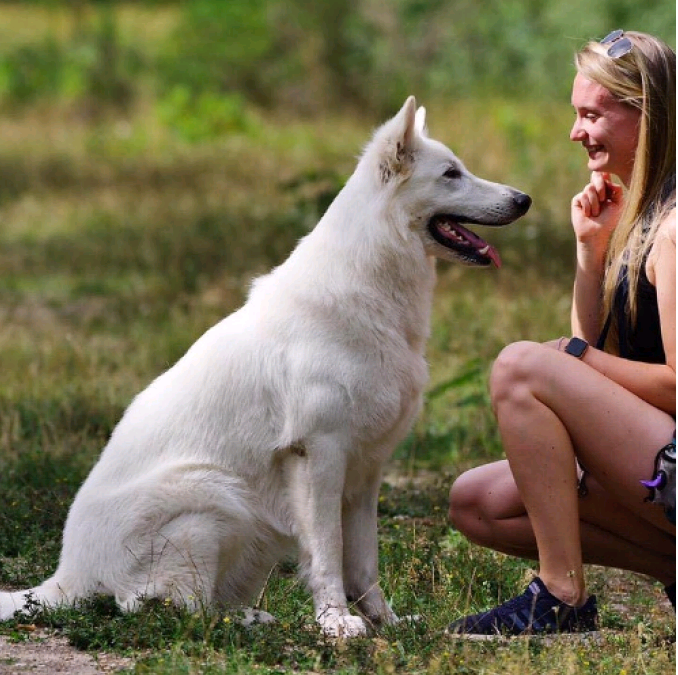
\includegraphics[width=0.769\textwidth]{resources/images/dog_woman.png}
    \end{minipage}%
    \fbox{
            \begin{minipage}{.45\textwidth}
                The picture shows two primary objects.
                  The first object is a dog, the second object is a woman.
                  The dog is white and has black eyes.
                  The woman is smiling and has blonde hair.
                  The woman is wearing shoes, shorts, a top, and a watch.
                  The shoes are blue.
                  The shorts are blue.
                  The top is black.
                  The watch is an Apple Watch.
                  In the background there is grass.
            \end{minipage}
    }
    \caption[Beispiel für eine generierte Erklärung]{Beispiel für eine generierte textuelle Beschreibung eines Bildes im GMAF.}
    \label{sec1:intro:subsec:motivation:fig:gmaf-explain-ui-dog-man-example}
\end{figure}
%\noindent
%\newline
Das \gmaf{} bietet hierfür ein umfangreiches Konzept zur Generierung von textuellen Beschreibungen von \mmir{}-Inhalten in für Menschen lesbarer und verständlicher Form.
Es ist allerdings wichtig anzumerken, dass dieses Konzept statistisch und rein mathematische Ansätze zur Generierung von natürlicher Sprache verfolgt, ohne dabei Methoden maschinellen Lernens zu verwenden.
Diese Ansätze generieren jedoch nur textuelle Beschreibungen auf eine statische Art und Weise.
Zudem können mit diesen Ansätzen keine anderen Formen, wie z.B visuelle Beschreibungen, außer Text generiert werden.
Es ist also erstrebenswert nach einer Lösung zu suchen, mit welcher man sich von diesen statischen Ansätzen lösen kann.
Ein anderer Ansatz, der in den letzten Monaten stark an Popularität gewonnen hat, ist die generative KI.
Generative KI scheint eine vielversprechende Alternative zu einem statischen, statistischen und rein mathematischen Ansatz zu sein.
\newline
Ließen sich mittels generativer KI tatsächlich \mmir{}-Prozesse erklären, so kann dies einen echten Mehrwert für Benutzer darstellen, da diese von präzisen Erklärungen oder visuellen Darstellungen profitieren würden.
Beispiele für Mehrwert für Benutzer können sein:
\begin{itemize}
    \item \textbf{Zeitersparnis.} Generative KI könnte anhand identifizierter Merkmale Datei(en) zusammenfassen und in kürzester Zeit präzise Beschreibungen der Datei(en) erstellen.
    Ein Benutzer müsste für diese Arbeit erheblich mehr Zeit aufwenden.
    \item \textbf{Überblick / Ordnung.} Generative KI könnte anhand identifizierter Merkmale in einer großen Kollektion an Dateien Zusammenhänge erkennen und dem Benutzer eine Beschreibung dieser Zusammenhänge bieten.
    Zusammenhänge können in diesem Fall Muster oder eine für den Benutzer versteckte bzw. nicht ersichtliche Ordnung innerhalb der Dateien sein.
    \item \textbf{Barrierefreiheit.} Es gibt bereits Programme, wie z.B. Screen Readers, die blinden Personen Beschreibungen von Bildern vorlesen.
    Nachteil ist, dass diese Programme abhängig von den im Bild eingebetteten Beschreibungen sind, und viele Bilder im Internet über keine eingebetteten Beschreibungen verfügen.
    Zusätzlich sind diese Beschreibungen meistens von Menschen verfasst \cite{google-ai-accessability}.
    \newline
    Generative KI könnte anhand identifizierter Merkmale Beschreibungen solcher Bilder generieren.
    Diese Beschreibungen könnten in weiteren Schritten von anderen Programmen, oder selbst wieder generativer KI verwendet werden, um diese vorzulesen.
    Auf diese Weise könnte echte Barrierefreiheit erreicht werden.
\end{itemize}

\FloatBarrier

%% Problembeschreibung
\subsection{Problembeschreibung}
\label{sec1:intro:subsec:problems}
Das \gmaf{} bietet bereits ein umfangreiches Konzept zur Erklärbarkeit von Prozessen des \mmir{}.
Die Ansätze, die in diesem Konzept verfolgt werden, sind statisch, in ihrer Anwendung begrenzt und ihre Erklärbarkeit vergleichsweise rudimentär.
In diesem Abschnitt werden diese Probleme angesprochen, umrissen und subsequent Problembeschreibungen definiert.

\subsubsection{Probleme in Bezug auf die Erklärbarkeit}
\label{sec1:intro:subsec:problems:pb:explain}
Das \gmaf{} bietet bereits Verfahren zur Erklärbarkeit von \mmir{}-Prozessen.
Die Ansätze, die mit diesen Verfahren umgesetzt werden, sind allerdings sehr statisch und basieren wiederum auf statistischen und rein mathematischen Ansätzen.
Noch dazu bieten diese Verfahren nur die Erklärbarkeit von \mmir{}-Prozessen anhand von Text.
Es ist allerdings wichtig anzumerken, dass Text nicht die einzige Form der Erklärbarkeit ist.
Eine andere Form der Erklärbarkeit kann mittels Bilder erzielt werden.
So lautet ein bekanntes Sprichwort: \enquote{\textit{Ein Bild sagt mehr als 1000 Worte}}.
Dieses Sprichwort will zum Ausdruck bringen, dass Bilder, im Vergleich zu Text, ebenfalls komplexe Sachverhalte und Wissen prägnant und in für Menschen verständlicher Form zum Ausdruck bringen können.
Ein Beispiel hierfür wäre eine Bauanleitung zu einem Lego-Set.
Ein Beispiel für eine Bauanleitung zum Bauen eines Osterkükens ist in \cref{sec1:intro:subsec:problems:fig:lego-instructions} zu sehen.
Die Bauanleitung veranschaulicht dabei die einzelnen Aufbauschritte durch fortwährende Nummerierung und Abbildungen.
\begin{figure}[!htb]
    \centering
    \copyrightbox[b]{
            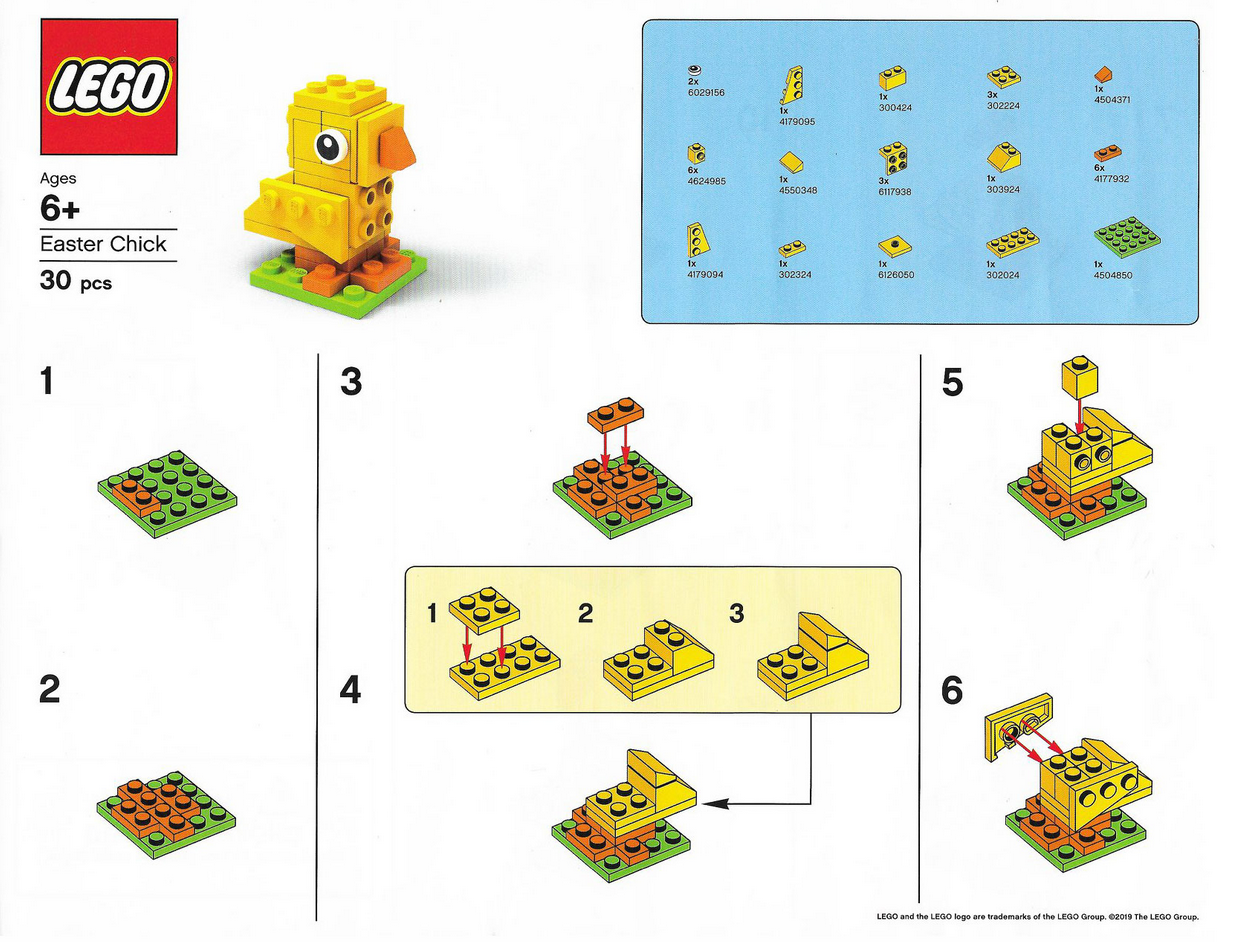
\includegraphics[width=0.8\linewidth]{resources/images/lego-instructions.png}
        }
        {%
        \textcolor{black}{%
            %Haftungsausschluss: \copyright{} 2023 Lego Gruppe - Diese Arbeit ist unabhängig und wurde von der LEGO Gruppe weder genehmigt noch gesponsert.
            Haftungsausschluss: LEGO \textsuperscript{\textregistered{}} und das LEGO Logo sind Marken der LEGO Unternehmensgruppe. 
            \newline
            \copyright{} 2023 Lego Gruppe. Diese Arbeit ist unabhängig und wurde von der LEGO Gruppe weder genehmigt, noch gesponsort.
        }
    }
    \caption{Bauanleitung für ein Lego-Set \cite{lego-easter-chick}.}
    \label{sec1:intro:subsec:problems:fig:lego-instructions}
\end{figure}

Ein konkretes Anwendungsbeispiel für die Erklärbarkeit in Form von Bildern wäre im Rahmen des \mmir{} die Generierung von Vorschaubildern für eine Textdatei.
\cref{sec1:intro:subsec:problems:fig:mmir-example-1} zeigt ein Beispiel für ein von Dall-E 2 \cite{dall-e-2} generiertes Vorschaubild für ein Gedicht über einen Schmetterling \cite{butterfly-poem}.
Anhand der in der Textdatei identifizierten Merkmale könnte eine generative KI, wie z.B Dall-E 2, ein Vorschaubild generieren, um somit den Inhalt des Textes visuell zu erklären.
\begin{figure}[!htb]
    \centering
    \resizebox{\textwidth}{!}{
        \begin{tikzpicture}
            \def\corner{5mm};
             \def\cornerradius{0.2mm};
             \def\lwidth{0.3mm};
             \def\h{3.5cm};
             \def\w{4.8cm};
             \def\nline{10};
             \def\iconmargin{1mm};
             \def\topmargin{2mm};
             \foreach[count=\i] \filename in {\textbf{Schmetterling}}
             {
               \coordinate (nw) at ($(0,0)$);
               \coordinate (ne0) at ($(nw) + (\w, 0)$);
               \coordinate (ne1) at ($(ne0) - (\corner, 0)$);
               \coordinate (ne2) at ($(ne0) - (0, \corner)$);
               \coordinate (se) at ($(ne0) + (0, -\h)$);
               \filldraw [-, line width = \lwidth, fill=white] (nw) -- (ne1) -- (ne2)
                [rounded corners=\cornerradius]--(se) -- (nw|-se) -- cycle;
               \draw [-, line width = \lwidth] (ne1) [rounded corners=\cornerradius]-- (ne1|-ne2) -- (ne2);
               \node [anchor=north west] at (nw) {\fontsize{10}{7}\selectfont \filename};
               \node [anchor=north west, text width=4.8cm] (poem) at ([yshift=-0.6cm]nw) {%
                  \begin{varwidth}{4.8cm}
                      \fontsize{6}{7.2}\selectfont
                      Fliege kleiner Schmetterling \newline
                      mach dir die Welt zu Eigen \newline
                      du kannst mit deiner Leichtigkeit \newline
                      uns noch so vieles zeigen \newline
                      zum Beispiel, dass es weiter geht \newline
                      auch wenn man lang im Dunkel steht \newline
                      am Lebensanfang nur gekrochen \newline
                      hast du die Freiheit nun gerochen \newline
                      du zeigst den Wandel uns im Leben \newline
                      so ist das Leben, Wandel eben. \newline
                      \vspace{\fill}
                  \end{varwidth}
               };
             }

             \draw[-latex, line width=0.7mm] (5.1, -1.7) -- node[above] {Dall-E 2} (7.5, -1.7);

             \node[] (img) at (10, -1.75) {
                \includegraphics[width=4.5cm]{resources/images/DALL·E 2023-04-19.png}
             };

             %\draw[-latex, line width=0.7mm] ([xshift=5mm]poem.east) -- node[above] {Dall-E 2} ([xshift=-5mm]img.west);

        \end{tikzpicture}
    }
    \caption[Beispiel für ein generiertes Vorschaubild]{Ein von Dall-E 2 generiertes Vorschaubild.}
    \label{sec1:intro:subsec:problems:fig:mmir-example-1}
\end{figure}

Ein Vorschaubild kann sich dann als sinnvoll erweisen, wenn viele Dateien zu verwalten sind und Benutzer nicht die Zeit haben diese einzeln zu durchforsten.
Durch einen kurzen Blick auf das Vorschaubild könnte ein Benutzer die Datei einordnen und sich besser zurechtfinden.

Ein weiteres Anwendungsbeispiel wäre die Gemeinsamkeit/Differenz aus einer Kollektion an Bildern.
Die als Gemeinsamkeit/Differenz identifizierten Merkmale könnten in diesem Beispiel ebenfalls konkret mittels eines Bildes kurz und prägnant visuell dargestellt werden.
Diese Art der visuellen Erklärung kann sich dann als sinnvoll erweisen, wenn viele Bilder auf ihre Merkmale hin untersucht werden sollen.
Ein Benutzer kann hier schnell den Überblick verlieren.

Statistische und rein mathematische Ansätze reichen für diese Beispiele nicht mehr aus.
Ein anderer, vielversprechender Ansatz, um die Erklärbarkeit von Prozessen des \mmir{} zu erreichen, liegt in generativer KI. Mittels generativer KI könnten anhand identifizierter Merkmale eigenständig neuartige Multimedia-Inhalte, wie Texte oder Bilder, erzeugt werden, die zur Erklärbarkeit von \mmir{}-Prozessen dienen könnten.

Je nach Anwendungsbereich variieren die Anforderungen an Erklärungen allerdings erheblich.
Somit ist ein weiterer wichtiger Aspekt die Anpassungsmöglichkeiten von Erklärungen in Abhängigkeit ihrer Anwendungsfälle.
%So wird \smmir{} für die Erkennung sicherheitsrelevanter Zustände im Bereich Automotive eingesetzt.
%Hier werden kurze, präzise Erklärungen benötigt.
%Im Gegensatz dazu steht der Bereich des Wissensmanagements, in welchem \smmir{} ebenfalls Anwendung für Fragestellungen findet.
%In diesem Bereich werden ausführliche Erklärungen benötigt.
So wird \smmir{} für die Erkennung sicherheitsrelevanter Zustände im Bereich der Automobilindustrie, auch Automotive genannt, eingesetzt \cite{jour-smmir}.
Sicherheitsrelevante Zustände in einem Kraftfahrzeug sind Zustände, die für eine reibungslose Fahrt und Funktion sorgen, oder unterstützend und im Sinne des Autofahrers eingreifen oder im Ernstfall zum Schutz von Insassen und Außenstehenden beitragen \cite{kfz-safety-states}.
Ein Beispiel für eine unterstützende Funktion kann in Form von HeadUp-Displays (HUD) gefunden werden und ist in \cref{sec1:intro:subsec:problems:fig:automotive-hud} zu sehen. Das HeadUp-Dispaly projiziert sicherheitsrelevante Informationen, wie z.B. die Geschwindigkeit auf die Windschutzscheibe.
\begin{figure}[htb]
    \centering
    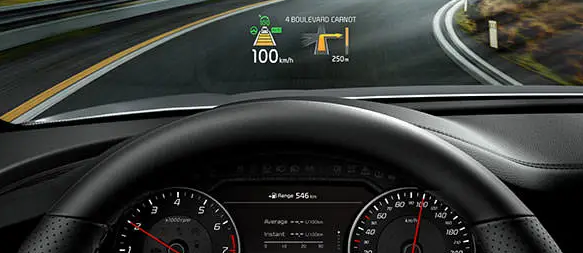
\includegraphics[width=0.9\textwidth]{resources/images/automotive-hud.png}
    \caption{HeadUp-Display in einem Kraftfahrzeug \cite{head-up-display}.}
    \label{sec1:intro:subsec:problems:fig:automotive-hud}
\end{figure}
Da im Bereich Automotive schnelle Entscheidungen getroffen werden müssen, werden hier kurze, präzise Erklärungen benötigt.
Es ist also in Bezug auf die Erklärbarkeit notwendig Eigenschaften, wie z.B. die Länge der Erklärung, anpassen zu können.
Das \gmaf{} bietet bereits eine Benutzungsschnittstelle, die es ermöglicht Anpassungen von textuellen Erklärungen vorzunehmen. Diese Benutzungsschnittstelle ist in \cref{sec1:intro:subsec:problems:fig:explain-ui} zu sehen und zeigt die Elemente, die zur Anpassung von textuellen Erklärungen vorgesehen sind.
\begin{figure}[htb]
    \centering
    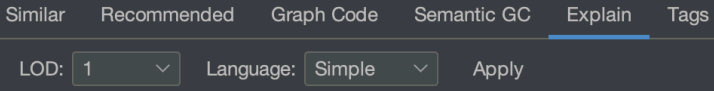
\includegraphics[width=0.7\textwidth]{resources/images/explain-ui.png}
    \caption{Benutzungsschnittstelle im \gmaf{} zum Anpassen von Erklärungen.}
    \label{sec1:intro:subsec:problems:fig:explain-ui}
\end{figure}
Diese Benutzungsschnittstelle bietet allerdings nur grobe Möglichkeiten zur Anpassung von textuellen Erlärungen, wie die Anpassung der Komplexität der textuellen Beschreibung.
Möglichkeiten zur Anpassung der Länge der textuellen Beschreibungen ermöglicht diese Schnittstelle zum Beispiel jedoch nicht. Schlussendlich kann in Bezug auf die Erklärbarkeit von \mmir{}-Prozessen folgende Problembeschreibung formuliert werden:

\problemstmt{} Generative KI ist aktuell nicht für die Erklärbarkeit von \mmir{}-Prozessen nutzbar.

\subsubsection{Probleme in Bezug auf die Integration}
\label{sec1:intro:subsec:problems:pb:integration}
Damit generative KI-Systeme aus identifizierten Merkmalen präzise und für Menschen verständliche Erklärungen generieren können, müssen die identifizierten Merkmale als Eingabedaten in die jeweiligen Systeme überführt werden.
Das \gmaf{} bietet keine Möglichkeiten zur Anbindung von Systemen, die generative KI anbieten, sowie kein Modell zur Übersetzung von identifizierten Merkmalen in Eingabedaten für entsprechende Systeme.
Folglich gibt es auch keine Modellierung, die die Anpassung der Eingabedaten ermöglicht, um die in \cref{sec1:intro:subsec:problems:pb:explain} benannten Modifikationen von Erklärungen zu ermöglichen.
Gelingt eine Integration von generativen KI-Systemen, so kann dies einen echten Mehrwert für Benutzer darstellen, sofern dadurch verbesserte und originellere Erklärungen von \mmir{}-Prozessen generiert werden.
Besonders die Möglichkeit, je nach Anforderung die Eingabedaten anzupassen, kann für Benutzer von Nutzen sein.
Schlussendlich kann in Bezug auf die Integration folgende Problembeschreibung formuliert werden:

\problemstmt{} Das \gmaf{} bietet keine Integration generativer KI.

\subsubsection{Allgemeine Zielsetzung}
\label{sec1:intro:subsec:objective}
Aus den in \cref{sec1:intro:subsec:problems:pb:explain} und \cref{sec1:intro:subsec:problems:pb:integration} beschriebenen Problembereichen lassen sich zwei direkte Probleme erfassen:
Die im \gmaf{} implementierten Konzepte zur Erklärung von \mmir{}-Prozessen sind noch sehr statisch und bieten nur Erklärungen in Form von Text, sowie die Integration besserer Lösungen zur Erklärbarkeit von \mmir{}-Prozessen.
Die Motivation dieser Arbeit besteht darin, dass die bereits implementierten Konzepte im \gmaf{} in Bezug auf die Erklärbarkeit von \mmir{}-Prozessen noch großen Raum für Verbesserung aufweisen.
Verbesserung wird sich durch das Anbinden von generativer KI versprochen, da generative KI in der Lage zu sein scheint auf kreative Weise neuartige Inhalte zu generieren.

Werden nun die Problembeschreibungen zusammengefasst, so wird das übergeordnete Ziel sichtbar:

\textit{Die im \gmaf{} implementierten Konzepte zur Erklärung von \mmir{}-Prozessen sollen durch \textbf{generative KI} abgelöst werden, um \textbf{bessere Erklärungen}, sowie \textbf{andere Formen von Erklärungen} zu ermöglichen.}

\clearpage
Anhand der in diesem Abschnitt beschriebenen Problembeschreibungen und des allgemeinen Ziels können nun im nächsten \cref{sec1:intro:subsec:research-questions} folgende Forschungsfragen formuliert werden. Im darauffolgenden \cref{sec1:intro:subsec:methodology-goals} wird genauer auf die Methodik dieser Arbeit, sowie die konkreteren Ziele eingegangen.

\subsection{Forschungsfragen}
\label{sec1:intro:subsec:research-questions}
Um die im vorigen Abschnitt definierten Problembeschreibungen zu adressieren, werden folgende Forschungsfragen definiert:
\begin{itemize}
    \item \researchquestion{} Kann generative KI für die Erklärbarkeit von \mmir{}-Prozessen genutzt werden?
    \item \researchquestion{} Wie lässt sich generative KI in das \gmaf{} integrieren?
\end{itemize}

\subsection{Methodik und Ziele}
\label{sec1:intro:subsec:methodology-goals}
Um die in \cref{sec1:intro:subsec:problems} identifizierten Probleme und subsequent die im vorigen \cref{sec1:intro:subsec:research-questions} formulierten Forschungsfragen strukturiert beantworten zu können, wird diese Arbeit auf der vielfach bewährten Methodik von Nunamaker \cite{nunamaker} aufbauen.
Die Methodik nach Nunamaker teilt ein zu lösendes Problem anhand von Recherche und Entwicklung in vier Phasen der Problemlösung auf.
\newline
Diese vier Phasen lauten:
\begin{enumerate}
    \setlength{\itemsep}{0pt}
    \item Beobachtungsphase
    \item Theoriebildungsphase
    \item Systementwicklungs - bzw. Implementierungsphase
    \item Experimentphase
\end{enumerate}
\begin{figure}[htb]
    \centering
    \resizebox*{0.75\textwidth}{!}{
        \begin{minipage}{\textwidth}
            \begin{tcolorbox}[
                enhanced, width=\textwidth, height=\textwidth, colback=white, colframe=black,
                overlay={
                    \tikzset{
                        exstyle/.style={-{Triangle[angle=90:6pt,length=3mm,fill=black]}}
                    }
                    \def\rad{\textwidth-2.5cm}
                    \node [circle, minimum size=\rad] (c) at ([yshift=-0.8cm]frame.center) {};
                    \def\labellist{
                          \shortstack{
                            \Large \textbf{Beobachtung} \\
                            \rule{3cm}{1pt} \\
                            \footnotesize
                            Umfragestudien, \\ 
                            \footnotesize
                            Fallstudien, \\
                            \footnotesize
                            Feldforschung
                          }, 
                          \shortstack{
                            \Large \textbf{Experiment} \\
                            \rule{3cm}{1pt} \\
                            \footnotesize
                            Computersimulationen,\\ 
                            \footnotesize
                            Feldexperimente, \\
                            \footnotesize
                            Laborexperimente
                          },
                          \shortstack{
                            \Large \textbf{Theorie} \\ \Large \textbf{Bildung} \\
                            \rule{3cm}{1pt} \\
                            \footnotesize
                            konzept. Rahmen-\\ 
                            \footnotesize
                            bedingungen, mathe\\
                            \footnotesize
                            matische Modelle\\
                            \footnotesize 
                            Methoden
                          }
                    }
                    
                    \foreach [count=\i] \x in \labellist {
                        
                        \node (n\i) [draw, fill=white, minimum size=0cm, inner sep=0mm, circle] at (c.\i*360/3+90) {
                            \scalebox{0.8}{
                                \x
                            }
                        };
                    }
                    \node (nm) [draw, fill=white, minimum size=0cm, inner sep=0mm, circle] at (c.center) {
                        \scalebox{0.8}{
                            \shortstack{
                                \Large \textbf{System} \\ \Large \textbf{Entwicklung} \\
                                \rule{3cm}{1pt} \\
                                \footnotesize
                                Produktentwicklung,\\ 
                                \footnotesize
                                Technologietransfer, \\
                                \footnotesize
                                Prototyping
                            }
                        }
                    };
                    \node [anchor=south east, rectangle, minimum width=4cm, rounded corners, text=white, fill=black, inner sep=1.7mm] at (frame.south east) {
                        \textbf{nach J. Nunamaker}
                    };

                    \draw[exstyle] (nm.200) -- (n1.40);
                    \draw[exstyle] (n1.25) -- (nm.215);

                    \draw[exstyle] (nm.340) -- (n2.140);
                    \draw[exstyle] (n2.155) -- (nm.325);

                    \draw[exstyle] (nm.{83}) -- (n3.{277});
                    \draw[exstyle] (n3.{263}) -- (nm.{97});

                    \draw[exstyle, bend left=41.5](n3.0) to (n2.60);
                    \draw[exstyle, bend left=41.5](n2.240) to (n1.300);
                    \draw[exstyle, bend left=41.5](n1.120) to (n3.180);

                    \draw[exstyle, bend right=41.5](n2.78) to (n3.342);
                    \draw[exstyle, bend right=41.5](n1.318) to (n2.222);
                    \draw[exstyle, bend right=41.5](n3.198) to (n1.102);

                    \node[circle, fill=white, draw, minimum size=1cm] at (n1.71) {1};
                    \node[circle, fill=white, draw, minimum size=1cm] at (n3.25) {2};
                    \node[circle, fill=white, draw, minimum size=1cm] at (nm.45) {3};
                    \node[circle, fill=white, draw, minimum size=1cm] at (n2.110) {4};
                }
            ]
            \end{tcolorbox}
        \end{minipage}
    }
    \caption{Phasen der Problemlösung nach Nunamaker \cite{nunamaker}.}
    \label{sec1:intro:subsec:methodology-goals:fig:nunamaker}
\end{figure}
In der Beobachtungsphase werden im Rahmen einer Recherche Informationen gesammelt.
In der Theoriebildungsphase werden Konzepte für Lösungen konzipiert und modelliert.
Die Systementwicklungs bzw. Implementierungsphase beschäftigt sich mit der Entwicklung von Lösungen, basierend auf den Theorien aus der Theoriebildungsphase bzw. Beobachtungen aus der Beobachtungsphase, und welche in der letzten Phase, der Experimentphase evaluiert werden können.
Diese Phasen sind eng miteinander verwoben, und jede Phase mündet mit seinem Ergebnis in den anderen Phasen und trägt zu diesen bei.
Durch die Methodik von Nunamaker wird sichergestellt, dass jedes Forschungsziel eindeutig einer Problembeschreibung zugeordnet werden kann.

Die Anwendung der Methodik nach Nunamaker führt für jede Forschungsfrage zu jeweils vier Forschungszielen, die in jeweils einem Unterkapitel behandelt werden.
Dies führt insgesamt zu acht Forschungsaufgaben, die mit dieser Arbeit behandelt werden.
Die anfängliche Planung der Forschungsziele ist in \cref{sec1:intro:table:research-questions} einsehbar.
Die Benennung der Forschungsaufgaben folgt einem einheitlichen Schema und ergibt sich aus dem Namen des jeweiligen Forschungsziels, erweitert durch einen Buchstaben als Anhängsel, z.B. \enquote{O}
 für \textit{Observation}/Beobachtung, \enquote{TB} für \textit{Theory Building}/Theoriebildung, \enquote{I} für \textit{Implementation}/Implementierung und \enquote{E} für \textit{Experiment}.
 \clearpage
{
    \def\arraystretch{1.1}%
    \begin{xltabular}{\linewidth}{
            @{}
            >{
                \hsize=0.15\linewidth
                \raggedright\arraybackslash
            }X
            >{
                \hsize=0.75\linewidth
                \raggedright\arraybackslash
            }X
            >{
                \hsize=0.1\linewidth
                \centering\arraybackslash
            }X
            @{}
    }

    % First Header

    \caption{Aufschlüsselung der Forschungsfragen auf Forschungsziele} 
    \label{sec1:intro:table:research-questions} \\
        
    \toprule
    \multicolumn{3}{
        >{
            \hsize=\linewidth\centering\arraybackslash
        }X
    }
    {
        \textbf{Forschungsfragen}
    } \\ 
    \midrule
         
    \textbf{FZ} & \multicolumn{1}{c}{\textbf{Beschreibung}} & \textbf{PB} \\ 
    \midrule
    
    \endfirsthead

    % Normal Head

    \toprule
    \multicolumn{3}{
        >{
            \hsize=\linewidth\centering\arraybackslash
        }X
    }
    {
        \textbf{Forschungsfragen}
    } \\ 
    \midrule
         
    \textbf{FZ} & \multicolumn{1}{c}{\textbf{Beschreibung}} & \textbf{PB} \\ 
    \midrule
    
    \endhead
        
    % Lower Rows

    \multicolumn{3}{
        >{
            \hsize=\linewidth\centering\arraybackslash
        }X
    }
    {
        \textbf{Erklärbarkeit von MMIR mittels generativer KI}
    } \\ \midrule

    FZ 1.1/O 
    & 
    Recherche zur Erklärbarkeit von MMIR mittels generativer KI
    & PB1 \\

    \midrule

    FZ 1.2/TB 
    & 
    Modellierung zur Erklärbarkeit von MMIR mittels generativer KI
    & PB1 \\

    \midrule

    FZ 1.3/I
    & 
    Implementierung zur Erklärbarkeit von MMIR mittels generativer KI
    & PB1 \\

    \midrule

    FZ 1.4/E 
    & 
    Experiment zur Erklärbarkeit von MMIR mittels generativer KI
    & PB1 \\

    \midrule

    \multicolumn{3}{
        >{
            \hsize=\linewidth\centering\arraybackslash
        }X
    }
    {
        \textbf{Integration generativer KI in das GMAF}
    } \\ \midrule

    FZ 2.1/O 
    & 
    Recherche zur Integration generativer KI in das GMAF
    & PB2 \\

    \midrule

    FZ 2.2/TB 
    & 
    Modellierung zur Integration generativer KI in das GMAF
    & PB2 \\

    \midrule

    FZ 2.3/I
    & 
    Implementierung zur Integration generativer KI in das GMAF
    & PB2 \\

    \midrule

    FZ 2.4/E 
    & 
    Experiment zur Integration generativer KI in das GMAF
    & PB2 \\
        
    \bottomrule 

    \end{xltabular}
}
\noindent
Um sicherzustellen, dass alle Forschungsziele durch den Inhalt dieser Arbeit abgedeckt werden, entspricht die Struktur dieses Dokuments direkt dem Ansatz nach Nunamaker.
Der Ansatz und Aufbau der Arbeit wird im nächsten Abschnitt behandelt.

\subsection{Ansatz und Aufbau der Arbeit}
\label{sec1:intro:subsec:approach-structure}
Die Struktur dieser Arbeit ergibt sich 1:1 aus der Methodik von Nunamaker \cite{nunamaker} und folgt seiner Modellierung.
Ein Überblick auf die Struktur dieser Arbeit und Nunamakers Ansatz ist in \cref{sec1:intro:subsec:approach-structure:fig:outline-nunamaker}.
Die entsprechenden Forschungsziele werden, je nach Phase der Modellierung nach Nunamaker, umgeordnet und in die jeweiligen Kapitel dieser Arbeit umgruppiert.
\clearpage
\begin{figure}[htb]
    \centering
    \newlength{\w}
    \setlength{\w}{0.9\textwidth}
    \resizebox*{\w}{!}{
        \begin{tikzpicture}

            \tikzset{
                exstyle/.style={-{Triangle[angle=90:6pt,length=3mm,fill=black]}},
                pbstyle/.style={-{Triangle[angle=90:3pt,length=1.5mm,fill=black]}}
            }

            \node[rectangle, minimum width=\w, minimum height=\w-2cm] (outline) {};

            \newlength{\nuna}
            \setlength{\nuna}{0.6\w}

            \node[anchor=south east, draw, rectangle, rounded corners, minimum width=\nuna, minimum height=\nuna] (nuna) at (outline.south east) {};

            \node [anchor=south east, draw, rectangle, rounded corners, text=white, fill=black] at (nuna.south east) {
                \scalebox{0.5}{
                    \textbf{nach J. Nunamaker}   
                }
            };

            \node[rectangle, rounded corners, minimum width=\nuna, minimum height=\nuna, inner sep=0mm] at ([yshift=-0.1cm]nuna.center) {
                \resizebox*{\nuna}{\nuna}{
                    \begin{tikzpicture}[transform shape]

                        \newlength{\radius}
                        \setlength{\radius}{\textwidth-2.5cm}
                        \node[circle, minimum size=\radius] (c) at (nuna.center) {};

                        \def\labellist{
                            \shortstack{
                                \Large \textbf{Beobachtung} \\
                                \rule{3cm}{1pt} \\
                                \footnotesize
                                Umfragestudien, \\ 
                                \footnotesize
                                Fallstudien, \\
                                \footnotesize
                                Feldforschung
                            }, 
                            \shortstack{
                                \Large \textbf{Experiment} \\
                                \rule{3cm}{1pt} \\
                                \footnotesize
                                Computersimulationen,\\ 
                                \footnotesize
                                Feldexperimente, \\
                                \footnotesize
                                Laborexperimente
                            },
                            \shortstack{
                                \Large \textbf{Theorie} \\ \Large \textbf{Bildung} \\
                                \rule{3cm}{1pt} \\
                                \footnotesize
                                konzept. Rahmen-\\ 
                                \footnotesize
                                bedingungen, mathe\\
                                \footnotesize
                                matische Modelle\\
                                \footnotesize 
                                Methoden
                            }
                        }

                        \foreach [count=\i] \x in \labellist {
                            \node (n\i) [draw, fill=white, minimum size=0cm, inner sep=0mm, circle] at (c.\i*360/3+90) {
                                \scalebox{0.8}{
                                    \x
                                }
                            };
                        }
                        \node (nm) [draw, fill=white, minimum size=0cm, inner sep=0mm, circle] at (c.center) {
                            \scalebox{0.8}{
                                \shortstack{
                                    \Large \textbf{System} \\ \Large \textbf{Entwicklung} \\
                                    \rule{3cm}{1pt} \\
                                    \footnotesize
                                    Produktentwicklung,\\ 
                                    \footnotesize
                                    Technologietransfer, \\
                                    \footnotesize
                                    Prototyping
                                }
                            }
                        };

                        \draw[exstyle] (nm.200) -- (n1.40);
                        \draw[exstyle] (n1.25) -- (nm.215);
    
                        \draw[exstyle] (nm.340) -- (n2.140);
                        \draw[exstyle] (n2.155) -- (nm.325);
    
                        \draw[exstyle] (nm.{83}) -- (n3.{277});
                        \draw[exstyle] (n3.{263}) -- (nm.{97});
    
                        \draw[exstyle, bend left=41.5](n3.0) to (n2.60);
                        \draw[exstyle, bend left=41.5](n2.240) to (n1.300);
                        \draw[exstyle, bend left=41.5](n1.120) to (n3.180);
    
                        \draw[exstyle, bend right=41.5](n2.78) to (n3.342);
                        \draw[exstyle, bend right=41.5](n1.318) to (n2.222);
                        \draw[exstyle, bend right=41.5](n3.198) to (n1.102);
                        
                    \end{tikzpicture}
                }
            };

            %\node[draw, rectangle, rounded corners, fill=gray!10] at ([xshift=1.9cm, yshift=1cm]n1.340) {
            %    \tiny Kapitel 2
            %};

            \newlength{\struc}
            \setlength{\struc}{0.47\w}

            \node[anchor=south west, draw, rectangle, rounded corners, minimum width=\struc, minimum height=3.74cm] (struc) at ([yshift=0.4cm]nuna.north west) {};

            \node[anchor=north, minimum width=\struc, draw, rectangle, rounded corners, text=white, fill=black] at (struc.north){
                \scalebox{0.5}{
                    \textbf{Struktur der Arbeit}
                }
            };

            \node[anchor=north west, draw, rectangle, rounded corners, fill=gray!10] (chap1) at ([xshift=0.1cm, yshift=-0.5cm]struc.north west) {
                \tiny Kapitel 1
            };

            \node[anchor=north west, draw, rectangle, rounded corners, fill=gray!10] (chap2) at ([xshift=0.1cm, yshift=-1.04cm]struc.north west) {
                \tiny Kapitel 2
            };

            \node[anchor=north west, draw, rectangle, rounded corners, fill=gray!10] (chap3) at ([xshift=0.1cm, yshift=-1.58cm]struc.north west) {
                \tiny Kapitel 3
            };

            \node[anchor=north west, draw, rectangle, rounded corners, fill=gray!10] (chap4) at ([xshift=0.1cm, yshift=-2.12cm]struc.north west) {
                \tiny Kapitel 4
            };

            \node[anchor=north west, draw, rectangle, rounded corners, fill=gray!10] (chap5) at ([xshift=0.1cm, yshift=-2.66cm]struc.north west) {
                \tiny Kapitel 5
            };

            \node[anchor=north west, draw, rectangle, rounded corners, fill=white] (chap6) at ([xshift=0.1cm, yshift=-3.2cm]struc.north west) {
                \tiny Kapitel 6
            };

            \node[anchor=west] at ([xshift=0.1cm]chap1.east) {
                \tiny Einleitung / Motivation
            };

            \node[anchor=west] at ([xshift=0.1cm]chap2.east) {
                \tiny Stand der Wissenschaft und Technik
            };

            \node[anchor=west] at ([xshift=0.1cm]chap3.east) {
                \tiny Modellierung / Design
            };

            \node[anchor=west] at ([xshift=0.1cm]chap4.east) {
                \tiny Implementierung
            };

            \node[anchor=west] at ([xshift=0.1cm]chap5.east) {
                \tiny Evaluierung
            };

            \node[anchor=west] at ([xshift=0.1cm]chap6.east) {
                \tiny Zusammenfassung / Fazit
            };

            \newlength{\chap}
            \setlength{\chap}{4.2cm}

            \node[anchor=south west, minimum width=\chap, minimum height=8cm, draw, rectangle, rounded corners] (chapter1) at (outline.south west) {};


            
            \node[anchor=center, draw, rectangle, rounded corners, fill=gray!10] (pbn) at ([yshift=-0.8cm]chapter1.north) {
                \tiny PB
            };

            \node[anchor=center, draw, rectangle, rounded corners, fill=gray!10] (pb1n) at ([xshift=-1cm, yshift=-2.8cm]chapter1.north) {
                \tiny PB1
            };

            \node[anchor=center, draw, rectangle, rounded corners, fill=gray!10] (pb2n) at ([xshift=1cm, yshift=-2.8cm]chapter1.north) {
                \tiny PB2
            };

            \node[anchor=center, draw, rectangle, rounded corners, fill=gray!10] (resq1) at ([xshift=-1cm, yshift=-4.5cm]chapter1.north) {
                \tiny FF1
            };

            \node[anchor=center, draw, rectangle, rounded corners, fill=gray!10] (resq2) at ([xshift=1cm, yshift=-4.5cm]chapter1.north) {
                \tiny FF2
            };

            

            \node[anchor=west, draw, rectangle, rounded corners, fill=gray!10] (resto) at ([xshift=-0.4cm, yshift=-5.85cm]chapter1.north) {
                \tiny FZ 1.1/O
            };

            \node[anchor=west, draw, rectangle, rounded corners, fill=gray!10] (resttb) at ([xshift=-0.4cm, yshift=-6.45cm]chapter1.north) {
                \tiny FZ 1.2/TB
            };

            \node[anchor=west, draw, rectangle, rounded corners, fill=gray!10] (resti) at ([xshift=-0.4cm, yshift=-7.05cm]chapter1.north) {
                \tiny FZ 1.3/I
            };

            \node[anchor=west, draw, rectangle, rounded corners, fill=gray!10] (reste) at ([xshift=-0.4cm, yshift=-7.65cm]chapter1.north) {
                \tiny FZ 1.4/E
            };

            \draw[pbstyle, line width=0.3mm] (pbn) -- (pb1n);
            \draw[pbstyle, line width=0.3mm] (pbn) -- (pb2n);

            \draw[pbstyle, line width=0.3mm] (pb1n) -- (resq1);
            \draw[pbstyle, line width=0.3mm] (pb2n) -- (resq2);
            
            \draw[pbstyle, line width=0.3mm] (resq1) |- (reste);
            \draw[pbstyle, line width=0.3mm] (resq1) |- (resti);
            \draw[pbstyle, line width=0.3mm] (resq1) |- (resttb);
            \draw[pbstyle, line width=0.3mm] (resq1) |- (resto);

            

            \node[align=left, anchor=north, minimum width=\chap, draw, rectangle, rounded corners, text=white, fill=black, text width=0.9\chap] (pb) at (chapter1.north){
                \tiny \textbf{Problem}
            };

            \node[align=left, anchor=north, minimum width=\chap, draw, rectangle, rounded corners, text=white, fill=black, text width=0.9\chap] (pbs) at ([yshift=-1.5cm]chapter1.north){
                \tiny \textbf{Problembeschreibungen}
            };

            \node[align=left, anchor=north, minimum width=\chap, draw, rectangle, rounded corners, text=white, fill=black, text width=0.9\chap] (resq) at ([yshift=-3.5cm]chapter1.north){
                \tiny \textbf{Forschungsfragen}
            };

            \node[align=left, anchor=north, minimum width=\chap, draw, rectangle, rounded corners, text=white, fill=black, text width=0.9\chap] (rest) at ([yshift=-5.04cm]chapter1.north){
                \tiny \textbf{Forschungsziele}
            };

            \node[anchor=center, draw, rectangle, rounded corners, fill=gray!10] at (pb.east) {
                \tiny Kap. 1
            };

            \node[anchor=center, draw, rectangle, rounded corners, fill=gray!10] at (pbs.east) {
                \tiny Kap. 1
            };

            \node[anchor=center, draw, rectangle, rounded corners, fill=gray!10] at (resq.east) {
                \tiny Kap. 1
            };

            \draw[exstyle, line width=0.6mm] (chap1.west) -| (chapter1.north);

            \draw[exstyle, line width=0.6mm] ([yshift=1cm]chapter1.south east) -- ([yshift=1cm]nuna.south west);



            \node[draw, rectangle, rounded corners, fill=gray!10] at ([xshift=-3.5cm, yshift=-1.2cm]nuna.center) {
                \tiny Kapitel 2
            };

            \node[draw, rectangle, rounded corners, fill=gray!10] at ([xshift=1.45cm, yshift=3.1cm]nuna.center) {
                \tiny Kapitel 3
            };

            \node[draw, rectangle, rounded corners, fill=gray!10] at ([xshift=1.3cm, yshift=0.2cm]nuna.center) {
                \tiny Kapitel 4
            };

            \node[draw, rectangle, rounded corners, fill=gray!10] at ([xshift=1.6cm, yshift=-2.3cm]nuna.center) {
                \tiny Kapitel 5
            };
            

        \end{tikzpicture}
    }
    \caption{Aufbau der Arbeit und Ansatz der Problemlösung nach Nunamaker \cite{nunamaker}.}
    \label{sec1:intro:subsec:approach-structure:fig:outline-nunamaker}
\end{figure}

Im Nachfolgenden werden die Kapitel jeweils einzelnen kurz beschrieben. Es wird genannt, welche Forschungsziele von welchem Typ abgearbeitet werden, und welche Aufgaben das entsprechende Kapitel jeweils übernimmt.
\begin{itemize}
    \setlength{\itemsep}{0pt}
    \item \textbf{\enquote{Kapitel 2 - Stand der Wissenschaft und Technik}} deckt alle Forschungsziele vom Typ \textit{Beobachtung} ab, und wird der Reihenfolge nach dem aktuellen Stand der Wissenschaft und Technik zusammenfassen, einführen und darstellen.
    \item \textbf{\enquote{Kapitel 3 - Modellierung}} deckt alle Forschungsziele vom Typ \textit{Theoriebildung} ab und beschreibt die Modellierung und das Design von Konzepten und Algorithmen zu vorgeschlagenen Problemlösungen.
    \item \textbf{\enquote{Kapitel 4 - Implementierung}} beschreibt die Implementierung von Modellen und Konzepten und deckt alle Forschungsziele vom Typ \textit{Systementwicklung bzw. Implementierung} ab.
    \item \textbf{\enquote{Kapitel 5 - Experiment}} deckt alle Forschungsziele vom Typ \textit{Experiment} ab und gibt eine detaillierte Beschreibung aller Ergebnisse.
\end{itemize}
\noindent
Um in dieser Arbeit einen wissenschaftlich formalen und korrekten Prozess zur Problemlösung anzuwenden, wurde die Modellierung nach Nunamaker eingeführt.
Dieser Modellierung folgend, wird eine klare Beziehung zwischen den Forschungszielen und den Forschungsfragen etabliert.
Dadurch wird sichergestellt, dass jedes Ergebnis, das in dieser Arbeit dargestellt wird, in direktem Bezug zu einer entsprechenden Forschungsfrage und einer Problembeschreibung steht und umgekehrt.
Des Weiteren folgt das Kapitel 3 \enquote{Modellierung} dieser Arbeit dem Ansatz \textit{User Centered System Design} nach Draper \cite{norman-draper-user-centered-system-design}, welches den Benutzer in den Mittelpunkt sämtlicher Modellierung und Planung stellt.
Die Modellierung und Planung wird auf der \textit{Unified Modeling Language} $(UML)$ \cite{uml} aufbauen.

%\subsection{Arbeits- und Zeitplan}
%\label{sec1:intro:subsec:work-time-plan}
%Der Arbeitsplan ist dem Ansatz der Arbeit nach strukturiert, sodass sich ebenfalls eine 1:1 Korrespondenz zwischen dem Ansatz der Arbeit, der Gliederung der Arbeit und dem Arbeitsplan ergibt.

%%\vspace*{\fill}
\begin{center}
\begin{turn}{-90}
\begin{sideways}
    \centering
    \begin{minipage}{\linewidth}
    \captionsetup{type=figure}
    \resizebox{\linewidth}{!}{
    \begin{ganttchart}[y unit title=0.6cm,
            y unit chart=0.8cm,
            x unit=0.64cm,
            vgrid,hgrid, 
            title label anchor/.style={below=-1.6ex},
            title left shift=.05,
            title right shift=-.06,
            title height=1,
            progress label text={},
            bar height=0.4,
            bar top shift=0.3,
            %bar node/.append style={anchor=north},
            bar label node/.append style={align=left, text width=7em, left=3pt},
            milestone label node/.append style={align=left, text width=9em},
            milestone inline label node/.append style={right=2ex,fill=white,fill opacity=.75,text opacity=1},
            flip/.style={milestone inline label node/.append style={left=2ex}},
            group right shift=0,
            group top shift=.6,
            group height=0.3]{1}{21}
    %labels
    \gantttitle{Arbeits- und Zeitplan}{21} \\
    %\gantttitle{April}{8}
    %\gantttitle{Mai}{8}
    %\gantttitle{Juni}{8}
    %\gantttitle{Juli}{8} \\
    \gantttitle[title label node/.append style={xshift=-23.7mm}]{Zeitraum}{0}
    %\foreach \x in {14,...,29} {
    %    \gantttitle{\x}{2}
    %}
    \gantttitle{1/9 - 10/9}{4}
    \gantttitle{11/9 - 1/10}{5}
    \gantttitle{2/10 - 29/10}{4}
    \gantttitle{30/10 - 19/11}{4}
    \gantttitle{20/11 - 1/12}{4}
    
    \\
        
    %tasks
    
    \ganttbar{Einleitung}{1}{4} \\
    \ganttbar{FZ 1.1/0}{5}{7} \\
    \ganttbar{FZ 2.1/0}{8}{9}
    \ganttmilestone[inline]{\textbf{Beobachtung}}{9} \\
    \ganttbar{FZ 1.2/TB}{10}{11} \\
    \ganttbar{FZ 2.2/TB}{12}{13}
    \ganttmilestone[inline]{\textbf{Modellierung}}{13} \\
    \ganttbar{FZ 1.3/I}{14}{15} \\
    \ganttbar{FZ 2.3/I}{16}{17} \\
    \ganttmilestone[inline,flip]{\textbf{Implementierung}}{17} \\
    \ganttbar{FZ 1.4/E}{18}{19} \\
    \ganttbar{FZ 2.4/E}{20}{21} \\
    \ganttmilestone[inline,flip]{\textbf{Experiment}}{21} 
        
    %relations 
    \ganttlink{elem0}{elem1}
    \ganttlink{elem1}{elem2}
    %\ganttlink{elem1}{elem3}
    \ganttlink{elem3}{elem4}
    \ganttlink{elem4}{elem5}
    \ganttlink{elem6}{elem7}
    \ganttlink{elem7}{elem8}
    \ganttlink{elem8}{elem10}
    %\ganttlink{elem9}{elem10}
    \ganttlink{elem10}{elem11}
        
    \end{ganttchart}
    }
    \captionof{figure}{Arbeits- und Zeitplan.} \label{sec1:intro:fig:gantt-chart-timeline}
    \end{minipage}
\end{sideways}
\end{turn}
\end{center}
\vspace*{\fill}

%\clearpage

\subsection{Zusammenfassung}
\label{sec1:intro:subsec:summary}
Das erste Kapitel dieser Arbeit hat allgemein in die Motivation des Themas eingeführt.
Eine kurze Beschreibung der aktuellen Entwicklung im Bereich Multimedia hat gezeigt, dass \mmir{} eine zunehmend wichtige Rolle spielt.
In diesem Zuge spielt auch die Erklärbarkeit von \mmir{}-Prozessen eine immer wichtigere Rolle.
Zwei Problembereiche konnten identifiziert werden, die mit dieser Arbeit adressiert werden.
Im Bereich der Erklärbarkeit bietet das \gmaf{} bereits umfangreiche Konzepte zur Erklärbarkeit von \mmir{}-Prozessen.
Diese Konzepte sind aber sehr statisch und in ihrer Anwendung stark eingeschränkt.
Hier gibt es allgemein großes Potenzial für Verbesserungen, die man sich durch das Anbinden generativer KI erhofft / verspricht.
Im Bereich der Integration konnte festgestellt werden, dass das \gmaf{} noch keine Anbindung für generative KI-Systeme bietet und hierfür eine geeignete Modellierung entwickelt werden muss.

Das Definieren von Problembeschreibungen, Forschungsfragen und Forschungszielen dient als formelle Grundlage für die Strukturierung dieser Arbeit.
Basierend auf der Modellierung nach Nunamaker folgt diese Arbeit einem wissenschaftlich anerkannten Ansatz bei der Darstellung der Forschungsergebnisse.
Um ein starkes Fundament für die Arbeit zu legen, wird im nächsten Kapitel ein detaillierter Überblick zum aktuellen Stand der Wissenschaft und Technik gegeben, in welchem die Ergebnisse der Forschungsziele vom Typ Beobachtung behandelt werden.


\section{Stand der Wissenschaft und Technik}
\label{sec2:sota}
Die voranschreitende Digitalisierung, die Entwicklung des Internets, Mobiltelefone, sowie die sozialen Medien und die damit einhergehenden enormen Datenmengen haben zu einer enormen Zunahme an Wissen, Standards und auch Forschung im Bereich des \mmir{} geführt \cite{swa_diss}. 
Im Bereich der Forschung spielt auch die Erklärbarkeit von \mmir{}-Prozessen eine zunehmend wichtige Rolle.
In einschlägiger Literatur, wie z.B \cite{swa_diss} wurde die Erklärbarkeit von \mmir{}-Prozessen bereits adressiert und es wurden Lösungsvorschläge und Konzepte entwickelt.

In diesem Kapitel wird, den Forschungszielen der Beobachtungsphase entsprechend, der aktuelle Stand der Wissenschaft und Technik bezogen auf ausgewählte Bereiche der Erklärbarkeit von Prozessen des \mmir{} beschrieben.
% Wie bin ich zu diesen Informationen gelangt?
% (Literaturrecherche, Internetrecherche (Publikationen vom Betreuer Wagenpfeil ...?))
Die in diesem Kapitel dargestellten Informationen wurden im Rahmen einer Literaturrecherche, speziell Publikationen, bezogen auf das GMAF und seine Technologien, sowie durch eine extensive Internetrecherche mit entsprechenden Stichworten zusammengetragen. 
Das Bezugssystem für diese Arbeit stellt das \gmaf{} dar.
Die für diese Arbeit relevanten Konzepte werden detailliert beschrieben, um so eine konkrete Vorlage, ein starkes Fundament, sowie eine scharfe Trennung zu den Phasen Modellierung, Implementierung und Experiment zu schaffen, die im weiteren Verlauf dieser Arbeit in den nachfolgenden Kapiteln Modellierung, Implementierung und Evaluierung folgen werden. 
Somit enthält dieses Kapitel alle nötigen Rechercheergebnisse, Beobachtungsergebnisse und damit Erkentnisse, die der Beantwortung der Forschungsfragen laut Ansatz dienlich sein sollen.
Der Methodik nach Nunamaker \cite{nunamaker} folgend, behandelt dieses Kapitel alle Forschungsziele vom Typ Beobachtung, entsprechend der identifizierten Problembeschreibungen aus dem \cref{sec1:intro:subsec:problems}.
In \cref{sec2:sota:subsec:fz-explainability} wird auf die Erklärbarkeit von MMIR mittels generativer KI eingegangen, welches vorhandene Technologien im Bereich MMIR, sowie generativer KI beinhaltet.
In \cref{sec2:sota:subsec:fz-integration} wird auf die Integration von generativer KI in das GMAF eingegangen, welches Technologien und technische Aspekte zur Integration beinhaltet.
In \cref{sec2:sota:subsec:eval-methodology} werden Methodiken zur Evaluierung vorgestellt, die später in Kapitel 5 im Rahmen von Experimenten Verwendung finden könnten.
Abschließend wird in \cref{sec2:sota:subsec:summary} eine Zusammenfassung der in diesem Kapitel erfassten Erkenntnisse und Ergebnisse gegeben.
Dieser Strukturierung folgend, wird im nächsten Abschnitt die erste Problembeschreibung adressiert.
Die Struktur dieses Kapitels ist in \cref{sec2:sota:table:structure} abgebildet.
{
    \def\arraystretch{1.1}%
    \begin{xltabular}{\linewidth}{
            @{}
            >{
                \hsize=0.25\linewidth
                \raggedright\arraybackslash
            }X
            >{
                \hsize=0.55\linewidth
                \raggedright\arraybackslash
            }X
            >{
                \hsize=0.2\linewidth
                \centering\arraybackslash
            }X
            @{}
    }

    % First Header

    \caption{Struktur dieses Kapitels.} 
    \label{sec2:sota:table:structure} \\
        
    \toprule

    \textbf{FZ} & \textbf{Kurze Beschreibung} & \textbf{Abschnitt} \\
    
    \midrule
    
    \endfirsthead

    % Normal Head

    \toprule

    \textbf{FZ} & \textbf{Kurze Beschreibung} & \textbf{Abschnitt} \\
    
    \midrule
    
    \endhead
        
    % Lower Rows

    FZ 1.1/O & Recherche: Erklärbarkeit \& generativer KI & \cref{sec2:sota:subsec:fz-explainability} \\
    FZ 2.1/O & Recherche: Integration generativer KI & \cref{sec2:sota:subsec:fz-integration} \\ \midrule
    Evaluierungsmeth. & Methodiken zur Evaluierung von Software & \cref{sec2:sota:subsec:eval-methodology} \\
    Zusammenfassung & Ergebnisse / Erkenntnisse & \cref{sec2:sota:subsec:summary} \\
        
    \bottomrule 

    \end{xltabular}
}

\subsection[FZ 1.1/O Erklärbarkeit von MMIR mittels generativer KI]{\texorpdfstring{FZ 1.1/O Erklärbarkeit von MMIR mittels \\ generativer KI}{FZ 1.1/O Erklärbarkeit von MMIR mittels generativer KI}}
\label{sec2:sota:subsec:fz-explainability}
Dieser Abschnitt gibt einen Überblick über ausgewählte Ergebnisse und Erkenntnisse aus der Forschung im Bereich der Erklärbarkeit von MMIR und deckt verschiedene Aspekte ab, die sich auf die erste Problembeschreibung beziehen.
Die Struktur dieses Abschnittes folgt einer logischen Abfolge.
Zuerst werden bereits vorhandene Technologien im Bereich der Erklärbarkeit von MMIR vorgestellt und erläutert. 
Dies trifft besonders auf Technologien in Bezug auf das GMAF zu, da das GMAF das Bezugssystem dieser Arbeit darstellt.
Im weiteren Verlauf wird dann auf generative KI eingegangen, Grundlagen werden erläutert, eine Auswahl an aktuellen Systemen generativer KI vorgestellt, sowie die Einschränkungen von generativer KI hervorgehoben.

\subsubsection{GMAF}
\label{sec2:sota:subsubsec:gmaf}
Das Generic Multimedia Analysis Framework (GMAF) \cite{gmaf_github} ist ein Framework, welches ausgewählte Technologien zum Verarbeiten verschiedener multimedialer Inhalte, wie Bilder, Videos oder Text nutzt und miteinander kombiniert \cite{ai-based-sem-ind-retr-soc, exp-mmfg}.
Beispiele für solche Technologien sind Verarbeitungssysteme zur Merkmalserkennung in Bildern (z.B zur Objekterkennung oder Erkennung von räumlichen Beziehungen mittels maschinellen Lernens).
Das GMAF bietet eine flexible und erweiterbare Architektur, mit welcher auf einfache Art und Weise neue Algorithmen oder Schnittstellen zur Merkmalserkennung im Form von Plugins in das GMAF integriert werden können \cite{exp-mmfg}.
Die von den Plugins extrahierten Merkmalen werden vom GMAF in einer zentralen Datenstrukturen zusammengefasst und vereint \cite{ai-based-sem-ind-retr-soc, jour-smmir}. \cref{sec2:sota:subsec:fz-explainability:fig:gmaf-overview} zeigt eine vereinfachte Übersicht der Architektur des GMAFs und die grundlegenden Komponenten. 
\begin{figure}[htb]
    \centering
    \resizebox{0.9\textwidth}{!}{
        \begin{tikzpicture}
            \tikzset{
                exstyle/.style={{Triangle[angle=90:4pt,length=2mm,fill=black]}-{Triangle[angle=90:4pt,length=2mm,fill=black]}}
            }
            \node[draw, rounded corners, rectangle, text width=6cm] (gmaf-core) {
                \shortstack[l]{
                    \textbf{GMAF Core} \\[1mm] Generic Multimedia \\ Analysis Framework
                }
            };

            \node[anchor=north west, draw, rounded corners, rectangle, text width=6cm] (gmaf-plugins) at ([xshift=2cm]gmaf-core.north east) {
                \begin{varwidth}{6cm}
                    \textbf{Plugins}

                    \begin{itemize}
                        \item Google Vision
                        \item Microsoft AI
                        \item Open AI
                        \item ...
                        \item EXIF
                        \item MPEG7
                    \end{itemize}
                \end{varwidth}
            };

            \node[draw, rounded corners, rectangle, text width=6cm, below=2cm of gmaf-core] (gmaf-mmfg) {
                \begin{center}
                    \textbf{Multimedia Feature Graph}
                    \newline
                    \textbf{(MMFG)}
                \end{center}
            };

            \draw[exstyle] (gmaf-core.south) -- node [fill=white] {\shortstack[c]{MMIR \\ Verarbeitung}} (gmaf-mmfg.north);

            \draw[exstyle] (gmaf-core.east) -- ++(2cm,0);
        \end{tikzpicture}
    }
    \caption{Vereinfachte Übersicht des GMAFs (ohne UI / API) nach \cite{jour-smmir}.}
    \label{sec2:sota:subsec:fz-explainability:fig:gmaf-overview}
\end{figure}
Die Plugins im GMAF können als ein Zusammenschluss aus Anbietern von semantischen Informationen betrachtet werden \cite{ai-based-sem-ind-retr-soc}.
Dieser Zusammenschluss produziert alle Daten, die notwendig sind, um ein Verzeichnis bzw. einen Index aus den semantischen Informationen zu generieren \cite{ai-based-sem-ind-retr-soc}.
Allgemein kann jedes durch ein Plugin identifizierte Merkmal einen Indizierungsbegriff darstellen und somit Teil des Indexes sein \cite{fast-effec-retr-large-collec}.
Da für gewöhnlich diese Begriffe strukturelle und semantische Beziehungen zueinander aufweisen, bietet sich zur Darstellung dieser Merkmale und ihren Beziehungen zueinander eine auf Graphen basierende Struktur an \cite{fast-effec-retr-large-collec}.
Diese Struktur wird durch den Multimedia Feature Graphen (MMFG) realisiert, welcher die in ihm gespeicherten semantischen Informationen in einem einheitlichen Modell repräsentiert \cite{fast-effec-retr-large-collec}.

%Im nächsten Abschnitt wird genauer auf die Datenstruktur der MMFGs eingegangen und die damit verbundenen Techniken werden detailliert erläutert.
Der nächste Abschnitt beschreibt die Datenstruktur der MMFGs, welche im Rahmen des GMAF eine zentrale Rolle einnehmen.
Zuerst wird die Grundstruktur der MMFGs beschrieben.
Im weiteren Verlauf wird dann in \cref{sec2:sota:par:explainability-of-mmfgs} die Erklärbarkeit von MMFGs thematisiert.
Darauffolgend wird in \cref{sec2:sota:par:processing-of-mmfgs} die Verarbeitung von MMFGs angesprochen, welcher den Übergang zu einer weiteren wichtigen Technologie, den Graph Codes, schafft.

\subsubsection{MMFG}
\label{sec2:sota:subsubsec:mmfg}
Der Multimedia Feature Graph (MMFG) ist ein Resultat des GMAFs und stellt für Prozesse innerhalb des GMAFs eine zentrale gemeinsame Ressource dar \cite{ai-based-sem-ind-retr-soc}.
Das grundlegende Konzept der MMFGs ist dabei eng verknüpft mit der Graphentheorie \cite{ai-based-sem-ind-retr-soc}.
Genauer lässt sich ein MMFG als ein gewichteter und gerichteter Graph mit attributierten Knoten und Kanten verstehen, der die aus Plugins identifizierten und extrahierten Merkmale multimedialer Inhalte in einer Graphenstruktur repräsentiert bzw. abbildet \cite{ai-based-sem-ind-retr-soc}.
Des Weiteren ist ein MMFG in der Lage Verbindungen zu Teilen anderer MMFGs aufzubauen, wodurch eine rekursive Struktur aus MMFGs entsteht, die Schleifen und Teilgraphen besitzen kann \cite{ai-based-sem-ind-retr-soc}.
Ein MMFG kann wie folgt definiert werden:
\begin{equation*}
    MMFG = (V, E)
\end{equation*}
Die Menge $V$ repräsentiert die Knoten in einem MMFG und stellt die identifizierten Merkmale dar.
Die Menge $E$ stellt wiederum die Verbindungen bzw. Beziehungen zwischen den Knoten bzw. Merkmalen dar.
Beide Mengen können anhand ihrer Attributierung in Unterklassen aufgeteilt werden.
Die Knotenmenge $V$ besteht aus folgenden Unterklassen: $V \in \{n,r,e,w,cn,t,m,s,l,p\}$.
%Die Bedeutung dieser Unterklassen wird im Folgenden genauer erläutert \cite{ai-based-sem-ind-retr-soc}:
Die folgende Aufzählung wurde aus \cite{ai-based-sem-ind-retr-soc} entnommen und erläutert die Bedeutung dieser Unterklassen:
\begin{itemize}
    \item \textbf{Nodes} $n_{1},...,n_{n}$ stellt wichtige Objekte, Aktivitäten oder Regionen in einer Datei dar. 
    $r$ ist die Wurzel des MMFGs und selbst wiederum ein Knoten.
    $e$ bezeichnet externe Knoten, die externe Informationen darstellen.
    Externe Informationen können aus anderen MMFGs oder anderen externen Systemen, wie dem Semantic Web stammen und so in den MMFG eingebunden werden.
    \item \textbf{Weight} $w_{1},...,w_{n}$ stellt die Gewichtung bzw. Relevanz eines Knoten in einem besonderen Kontext dar. 
    So können Objekte, abhängig vom Kontext und Gewichtung, unterschiedliche Bedeutungen in Bezug auf die gesamte Datei besitzen.
    \item \textbf{Childnodes} $cn_{1},...,cn_{n}$ sind Objekte, die in einer untergeordneten hierarchischen Beziehung zu anderen Objekte stehen.
    Diese Objekte entstehen durch wiederholte bzw. rekursive Anwendung des GMAFs auf bereits identifizierte Merkmale.
    Ein Beispiel für diese rekursive Anwendung ist \textit{Person $\rightarrow$ Body $\rightarrow$ Arm $\rightarrow$ Watch} und kann in \cref{sec2:sota:subsec:fz-explainablity:fig:mmfg-example} eingesehen werden.
    \item \textbf{TechnicalAttributes} $t_{1},...,t_{n}$ stellen nicht semantische Informationen eines Knoten dar.
    Beispiel für ein technisches Attribut kann die Abgrenzung eines Merkmals in einem Bild sein.
    Diese Abgrenzung wird in Form eines Rechtecks notiert ($x$: 468, $y$: 176, $width$: 28, $height$: 12).
    \item \textbf{GeneralMetadata} $m$ stellt die Metadaten der Multimedia-Datei dar. 
    Mit Metadaten bezeichnet man Daten, die andere Informationen beschreiben und können durch EXIF oder MPEG7 identifiziert werden.
    Die Metadaten eines Buches könnten so z.B. der Name des Autors, Auflage oder das Erscheinungsjahr sein.
    \item \textbf{Location} $l_{1},...,l_{n}$ stellt Speicherorte dar.
    Dies kann der Speicherort der ursprünglichen Multimedia-Datei, aber auch von Kopien, unterschiedlichen Auflösungen oder Teilen der Datei sein.
    \item \textbf{SynonymInformation} $s_{1},...,s_{n}$ verweist auf Synonyme eines Begriffes.
    \item \textbf{Security and Privacy} $p$ stellt die Sicherheitseigenschaften einer Datei dar.
    Beispiel für so eine Sicherheitseigenschaft ist eine Zugriffskontrollliste (engl. access control list).
    Auf diese Weise kann der Umgang mit vertraulichen Daten sichergestellt werden.
\end{itemize}
Auch die Kanten in $E$ besitzen Unterklassen und können in folgende Unterklassen unterteilt werden: $E \in \{cr,sr,sn,mm,al\}$.
%Analog zu den Knoten werden im Folgenden diese Unterklassen genauer erläutert \cite{ai-based-sem-ind-retr-soc}:
Die folgende Aufzählung wurde aus \cite{ai-based-sem-ind-retr-soc} entnommen und erläutert, analog zu den Knoten, die Bedeutung der Unterklassen der Kanten:
\begin{itemize}
    \item \textbf{Composition Relationsip} $cr_{1},...,cr_{n}$ drückt das Verhältnis in dem zwei Objekte miteinander stehen aus.
    Beispiele für solche Beziehungen können \enquote{verbunden mit (engl. attached to)}, \enquote{ein Teil von (engl. part of)} oder \enquote{bezogen auf (engl. related to)} sein.
    Diese Beziehungen werden vom GMFA durch rekursives Berechnen der Abgrenzungen von Merkmalen und deren Distanzen zueinander berechnet.
    \item \textbf{Sematic Relationship} $sr_{1},...,sr_{n}$ verbindet einen Knoten mit einem externen Knoten aus einem externen System, wie z.B. dem Semantic Web.
    \item \textbf{SynonymLinks} $sn_{1},...,sn_{n}$ verweist auf Informationen zu Synonymen.
    \item \textbf{MMFGLinks} $mm_{1},...,mm_{n}$ stellt Verbindungen zu anderen MMFGs dar.
    \item \textbf{AssetLinks} $al_{1},...,al_{n}$ zeigt auf Knoten, die Speicherorte darstellen.
\end{itemize}
\cref{sec2:sota:subsec:fz-explainability:fig:mmfg-real-example} zeigt die Visualisierung eines MMFGs durch yEd.
Dieser MMFG besitzt 185 Knoten und 222 Kanten.
Aufgrund des steigenden Level Of Detail (LOD) vieler multimedialer Inhalte, wie z.B. durch höhere Auflösung von Bildern, steigt die Anzahl der Knoten und Kanten in MMFGs drastisch \cite{ai-based-sem-ind-retr-soc}.
In der Praxis können MMFGs tausende Knoten und Kanten aufweisen \cite{jour-smmir}.
In diesen Maßstäben ist eine Visualisierung eines MMFGs auf sinnvolle Weise kaum noch möglich.
Das Hauptaugenmerk der MMFGs liegt nicht darauf für Menschen lesbar, darstellbar oder verständlich zu sein, sondern anhand ihrer Graphenstruktur geeignete Verarbeitung der Merkmale zu ermöglichen \cite{ai-based-sem-ind-retr-soc}.

\begin{figure}[htb]
    \centering
    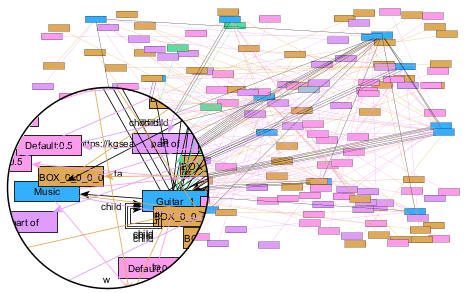
\includegraphics{resources/images/mmfg-example.png}
    \caption{Visualisierung eines MMFGs durch yEd.}
    \label{sec2:sota:subsec:fz-explainability:fig:mmfg-real-example}
\end{figure}
\cref{sec2:sota:subsec:fz-explainablity:fig:mmfg-example} zeigt einen simplen $MMFG_{ex}$. 
Die Knoten \textit{Person, Body, Arm, Watch} repräsentieren identifizierte Merkmale, \textit{Clock} ist ein Synonym für \textit{Watch} und \textit{attached to} verweist auf eine Beziehung zwischen \textit{Arm} und \textit{Watch}.

\begin{figure}
    \centering
    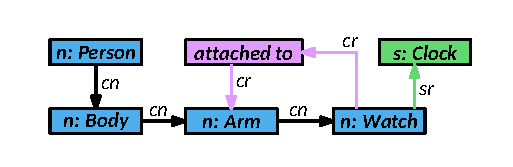
\includegraphics[width=0.7\textwidth]{chapter/chapter_2/mmfg-ex.eps}
    \caption{Beispiel für einen $MMFG_{ex}$.}
    \label{sec2:sota:subsec:fz-explainablity:fig:mmfg-example}
\end{figure}

\paragraph{Erklärbarkeit von MMFGs}
\label{sec2:sota:par:explainability-of-mmfgs}
Um Erklärbarkeit von MMFGs zu erreichen, muss die technische Darstellung der Merkmale in eine für Menschen verständliche Bedeutung überführt werden.
Das Überbrücken dieser Lücke ist nicht in einem einzigen Schritt machbar. 
Es benötigt mehrere Schritte um diese Lücke zu schließen.
In einem ersten Zwischenschritt muss die Lücke zwischen der technischen Darstellung der Merkmale und ihrer semantischen Darstellung überbrückt werden.
Hierzu wird ein formaler und für Maschinen lesbarer Ansatz zur Erweiterung von MMFGs benötigt \cite{towards_auto_sem_expl_mmfg}.
In verwandten Arbeiten, wie \cite{towards_auto_sem_expl_mmfg}, wurden umfangreiche Konzepte entwickelt und beschrieben, die in der Lage sind durch Erweiterungen von MMFGs Erklärbarkeit zu erreichen.
Das Überbrücken der Lücke zwischen der technischen Darstellung der Merkmale und ihrer semantischen Darstellung gelingt mit einer semantischen Erweiterung.
Eine semantische Erweiterung von MMFGs kann durch das Anbinden eines externen Informationssystems, wie z.B. dem Semantic Web \cite{sem-web}, erreicht werden.
Durch das Definieren und Anwenden einer formalen kontextfreien Phrasenstruktur-Grammatik \cite{hausser-ps-grammar} in Kombination mit einer semantischen Erweiterung sind die Darstellungen von MMFGs nicht nur für Menschen lesbar, sondern es können auch für Menschen verständliche, sowie lesbare und auf natürlicher Sprache basierende Ausdrücke generiert werden.
Diese Erweiterungen ermöglichen formale semantische Darstellungen und schaffen die Grundlage für auf natürlicher Sprache basierende Erklärungen.
Diese Erweiterungen von MMFGs zu formalen semantischen Darstellungen führen zu Semantischen Multimedia Feature Graphen (SMMFGs) \cite{towards_auto_sem_expl_mmfg}, sowie zu Erklärbaren Semantischen Multimedia Feature Graphen (ESMMFGs) \cite{towards_auto_sem_expl_mmfg}.

Jeder auf natürlicher Sprache basierende Ausdruck, der mit solch einer Grammatik generiert wird, ist inhaltlich \textit{korrekt}, da es nur die ursprünglichen identifizierten Merkmale in einer formalen und für Menschen lesbaren Form darstellt \cite{towards_auto_sem_expl_mmfg}.
Auf diese Weise kann jedes Element eines MMFG bzw. identifizierte Merkmal strukturell und semantisch dargestellt werden \cite{towards_auto_sem_expl_mmfg}.
Des Weiteren bieten sich anhand der Grammatik und ihrer Produktionsregeln unbegrenzte Möglichkeiten zur Konstruktion natürlicher Ausdrücke \cite{towards_auto_sem_expl_mmfg}.
Durch Anpassungen der Produktionsregeln können Applikationen individuell die Konstruktion natürlicher Ausdrücke bestimmen \cite{towards_auto_sem_expl_mmfg}.
Anhand dieser Techniken können bereits gute Ergebnisse bzw. Erklärungen erzielt werden.
Besonders textbasierte Dokumente können mit dieser Herangehensweise erklärt werden, da die Struktur des MMFGs der Struktur des Dokuments folgt \cite{towards_auto_sem_expl_mmfg}.
Dies gilt allerdings nicht für andere Multimedia-Dateien, wie z.B. Bildern. 
Für diese Dateitypen bleibt die Reihenfolge der konstruierten Sätze zufällig \cite{towards_auto_sem_expl_mmfg}.

Wichtig anzumerken ist, dass diese Konzepte ohne maschinelles Lernen auskommen und einen rein mathematischen und statistischen Ansatz verfolgen, um Erklärungen anhand identifizierter Merkmale zu generieren \cite{towards_auto_sem_expl_mmfg}.

\paragraph{Verarbeitung von MMFGs}
\label{sec2:sota:par:processing-of-mmfgs}
Der steigende Detaillierungsgrad (LOD) vieler multimedialer Inhalte führt zu einem Anstieg in der Anzahl an Elementen in einem MMFG \cite{exp-mmfg}.
So können in der Praxis MMFGs tausende Knoten und Kanten enthalten \cite{ai-based-sem-ind-retr-soc}.
Ein höherer Detaillierungsgrad und eine höhere Anzahl an Elementen in einem MMFG stärkt zwar die Wirksamkeit der Ergebnisse von Berechnungen eines MMFGs, wie z.B der Berechnung der Ähnlichkeit zweier MMFGs, sorgt aber allgemein auch für eine komplexere Graphenstruktur \cite{fast-effec-retr-large-collec}.
Diese Eigenschaft von MMFGs birgt eine Reihe von Problemen.
Zum einen ist die Umsetzung aktueller Algorithmen, wie z.B. zur Bestimmung der Ähnlichkeit von MMFGs, auf rechenschwachen Systemen, wie z.B Smartphones, mit dieser Anzahl an Knoten und Kanten aufgrund Speicherplatz und Laufzeitbegrenzungen nicht einfach zu handhaben und zum anderen sind aktuelle Algorithmen, die auf dem Durchlaufen eines Graphen basieren, wie z.B die Bestimmung der Ähnlichkeit zweier MMFGs, bei solch einer Anzahl an Knoten und Kanten nicht mehr effizient und zudem sehr rechenaufwendig \cite{fast-effec-retr-large-collec}.

Mathematisch betrachtet können Graphen durch ihre Adjanzenzmatrix dargestellt werden \cite{fast-effec-retr-large-collec}.
Basierend auf einer Adjanzenzmatrix können weitere Umformungen und Berechnungen durchgeführt werden \cite{fast-effec-retr-large-collec}. Ein Beispiel hierfür ist die Umwandlung eines Graphen in einen n-dimensionalen Vektorraum. Auf diesem Vektorraum können dann wiederum weitere Berechnungen durchgeführt werden.
Speziell für gewichtete Graphen, zu welchen auch per Definition MMFGs zählen, werden in der Regel Matrizen angewandt \cite{fast-effec-retr-large-collec}.
Diese Matrizen erweitern eine Adjanzenzmatrix um die Gewichtung der Kanten.
Im weiteren Verlauf dieser Arbeit werden diese Matrizen auch Wertungsmatrizen (engl. valuation matrices) genannt.
Basierend auf diesen Darstellungen können mathematische Konzepte angewandt werden.
Ein Beispiel für so ein mathematisches Konzept ist die Anwendung der Eigenwert-Methode, durch welche eine auf Merkmale bezogene Ähnlichkeitsberechnung von Adjanzenzmatrizen durchgeführt werden kann \cite{fast-effec-retr-large-collec}.
Die Eigenwert-Methode reduziert eine quadratische Matrix $M$ auf eine einfache rationale Zahl $\lambda$ unter der Annahme $\exists~\Vec{v}: M \cdot \Vec{v} = \lambda \cdot \Vec{v}$ \cite{fast-effec-retr-large-collec}.
Auf diese Weise können Ähnlichkeitsberechnungen auf $\lambda$ anstatt der gesamten Matrix $M$ durchgeführt werden \cite{fast-effec-retr-large-collec}.
Allerdings weisen viele dieser Algorithmen eine polynomielle Laufzeit von $\mathcal{O}((n + e)^2)$ oder gar exponentielle Laufzeit auf (hierbei verweist $n$ auf die Anzahl der Knoten und $e$ auf die Anzahl der Kanten) \cite{fast-effec-retr-large-collec}.
Um effektive und effiziente Verarbeitungen, wie z.B. Abfragen, für große Datenstrukturen und Sammlungen multimedialer Inhalte, wie einem MMFG, zu ermöglichen, müssen effizientere Algorithmen, wie zur Bestimmung der Ähnlichkeit von MMFGs, die mit komplexeren Graphenstrukturen umgehen können, eingesetzt werden \cite{fast-effec-retr-large-collec}.

Im nächsten Abschnitt wird eine Projektion eines Graphen in einen zweidimensionalen Vektorraum, sowie entsprechende Algorithmen vorgestellt.
Diese Projektion stellt eine Erweiterung der Wertungsmatrix eines Graphen dar und ermöglicht statt einer exponentiellen Komplexität der Laufzeit eine lineare Laufzeitkomplexität von $\mathcal{O}(n+e)$ und unterstützt zudem ein höheren Detaillierungsgrad von MMFGs \cite{fast-effec-retr-large-collec}.
Das Konzept dieser Projektion wird im weiteren Verlauf der Arbeit als Graph Code \cite{gc-2d-proj-mmfg} bezeichnet.


\subsubsection{Graph Codes}
\label{sec2:sota:subsubsec:graph-codes}
In diesem Abschnitt werden die mathematischen und algorithmischen Konzepte der Graph Codes beschrieben.
Zuerst werden die Grundlagen von Graph Codes beschrieben.
Diese Grundlagen umfassen des Weiteren die in \cref{sec2:sota:par:gc-encoding} beschriebene Codierung von Graph Codes, sowie die in \cref{sec2:sota:par:gc-vocabulary-dictionary} beschriebenen technischen Eigenschaften, wie Vokabular und Wörterbücher von Graph Codes.
In \cref{sec2:sota:par:gc-similiarity} wird dann die Ähnlichkeit von Graph Codes behandelt.

Graph Codes sind eine Projektion eines MMFG in einen zweidimensionalen Raum \cite{gc-2d-proj-mmfg}.
Dabei basieren Graph Codes auf Operationen auf der Adjanzenzmatrix eines Graphen und können allgemein, per Prinzip, auf jede Art von Graphen angewendet werden.
Allerdings wurden Graph Codes spezifisch für MMIR entwickelt.
Graph Codes werden eingesetzt, um MMFGs zu transformieren und in einer Form darzustellen, die schnelleres und effizienteres MMIR ermöglicht \cite{fast-effec-retr-large-collec}.
Grundlage dieser Umformung ist ein Algorithmus zur Codierung eines MMFG.
Dieser Algorithmus nimmt die Wertungsmatrix $WM$ eines MMFGs als Eingabe \cite{gc-2d-proj-mmfg}.
Um die grundlegenden Konzepte von Graph Codes vorzustellen, wird das Beispiel $MMFG_{ex}$ aus \cref{sec2:sota:subsec:fz-explainablity:fig:mmfg-example} als Basis benutzt.
Eine Wertungsmatrix enthält jeweils eine Zeile und Spalte für einen Knoten in einem MMFG.
Aufgrund dessen ist eine Wertungsmatrix auch eine quadratische Matrix.
Eine gerichtete Kante zwischen zwei Knoten $n_1$ und $n_2$ wird in der Wertungsmatrix durch ihre Gewichtung oder durch den Wert 1 im Eintrag $(n_1,n_2)$ der Wertungsmatrix $WM$ dargestellt.

Die Knoten \textit{Person, Body, Arm, Watch, Clock, attached to} des Beispiels $MMFG_{ex}$ werden in der Diagnonalen der Wertungsmatrix ebenfalls durch den Wert 1 dargestellt.
Dies führt zu der in \cref{sec2:sota:subsec:fz-explainablity:fig:mmfg-valuation-matrix} dargestellten Wertungsmatrix.

%\begin{figure}[htb]
    \centering
    \resizebox{0.8\textwidth}{!}{
        \begin{tikzpicture}
            \node (tabl) {
                \begin{tabular}{rcccccc}
                     &  \begin{turn}{90}Person\end{turn}& \begin{turn}{90}Body\end{turn} & \begin{turn}{90}Arm\end{turn} & \begin{turn}{90}Watch\end{turn} & \begin{turn}{90}Clock\end{turn} & \begin{turn}{90}attached to $~$\end{turn} \\ \hline
                    Person      & 1 & 1 & 0 & 0 & 0 & 0 \\ 
                    Body        & 0 & 1 & 1 & 0 & 0 & 0 \\
                    Arm         & 0 & 0 & 1 & 1 & 0 & 0 \\ 
                    Watch       & 0 & 0 & 0 & 1 & 1 & 1 \\ 
                    Clock       & 0 & 0 & 0 & 0 & 1 & 0 \\ 
                    attached to & 0 & 0 & 1 & 0 & 0 & 1
                \end{tabular}
            };

            \node[anchor=south west] (wm) at([xshift=5mm]tabl.south east) {
                \shortstack[c]{
                    $WM(MMFG_{ex}) = $\\
                    \vspace*{1.5mm} \\
                    $\begin{pmatrix}
                    1 & 1 & 0 & 0 & 0 & 0  \\
                    0 & 1 & 1 & 0 & 0 & 0  \\
                    0 & 0 & 1 & 1 & 0 & 0  \\
                    0 & 0 & 0 & 1 & 1 & 1  \\
                    0 & 0 & 0 & 0 & 1 & 0  \\
                    0 & 0 & 1 & 0 & 0 & 1  \\
                    \end{pmatrix}$
                }
            };

            %\node[draw, fit=(tabl)(wm)] {};
        \end{tikzpicture}
    }
    \caption{Wertungsmatrix des Beispiels $MMFG_{ex}$.}
    \label{sec2:sota:subsec:fz-explainablity:fig:mmfg-valuation-matrix}
\end{figure}
\begin{figure}[htb]
    \centering
    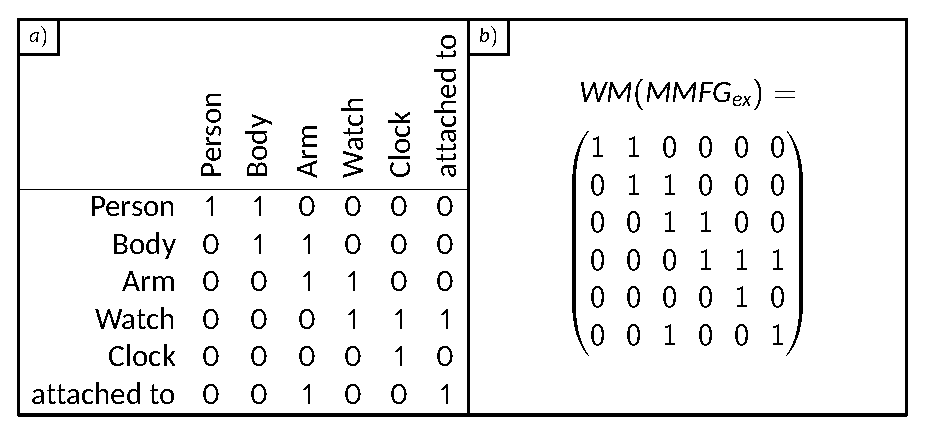
\includegraphics[width=\textwidth]{chapter/chapter_2/valuation-matrix-a-b.eps}
    \caption{Wertungsmatrix des Beispiels $MMFG_{ex}$ in a) Tabellenform und b) Form einer Matrix.}
    \label{sec2:sota:subsec:fz-explainablity:fig:mmfg-valuation-matrix}
\end{figure}

\paragraph{Codierung von Graph Codes}
\label{sec2:sota:par:gc-encoding}
Graph Codes wenden eine Funktion $f_{enc}$ zur Codierung von Informationen in einem MMFG an.
Diese Funktion codiert die Informationen zu den Typen der Knoten oder Kanten und ihren entsprechenden Attributen.
Hierzu werden für alle Einträge bzw. Felder in der Wertungsmatrix $WM$, die nicht null sind, numerische Werte berechnet.
Die Funktion $f_{enc}$ zur Codierung dieser Informationen kann von Applikationen je nach ihren jeweiligen Anforderungen angepasst werden \cite{gc-2d-proj-mmfg}.
Eine beispielhafte Codierung kann wie folgt lauten: Knoten = 1, Blatt = 2, Kindsbeziehung = 3, Synonymbeziehung = 4, Beziehung = 5, Knoten (räumliche Beziehung) = 6, Knoten (Synonym) = 7.
Angewandt auf das Beispiel $MMFG_{ex}$ führt diese Codierung zu folgender in \cref{sec2:sota:subsec:fz-explainablity:fig:mmfg-valuation-matrix-enc} a-b) dargestellten codierten Wertungsmatrix $WM_{enc}$ bzw. Graph Code $GC_{ex}$.
Die Farben der Einträge in \cref{sec2:sota:subsec:fz-explainablity:fig:mmfg-valuation-matrix-enc} entsprechen der Färbung der Knoten aus \cref{sec2:sota:subsec:fz-explainablity:fig:mmfg-example}. 
Die dazugehörigen Beziehungen sind ebenfalls entsprechend gefärbt.
\cref{sec2:sota:subsec:fz-explainablity:fig:mmfg-valuation-matrix-enc} c) hingegen zeigt den durch das GMAF generierten Graph Code $GC_{ex}$ des Beispiels $MMFG_{ex}$.
Es sei angemerkt, dass die Unterschiede zwischen dem Graph Code $GC_{ex}$ aus \cref{sec2:sota:subsec:fz-explainablity:fig:mmfg-valuation-matrix-enc} a-b) und \cref{sec2:sota:subsec:fz-explainablity:fig:mmfg-valuation-matrix-enc} c) durch die vom GMAF eigens definierte Fuktion $f_{enc}$ zu Stande kommen.
Des Weiteren inkludiert das GMAF die Synonym-Knoten $Clock$ und $attached~to$ nicht in seiner Abbildung.
Die Beziehung $attached~to$ wird im GMAF durch den Eintrag $(Arm,Watch)$ im Graph Code $GC_{ex}$ dargestellt.
Hier wird eine feinere Differenzierung der räumlichen Beziehung vorgenommen und durch den Wert 17 dargestellt.
Durch komplexere Funktionen zur Codierung können Attribute, Gewichtung oder auch andere Informationen in einem MMFG codiert und durch beliebige Zahlen dargestellt werden, welche im weiteren Verlauf einer Verarbeitung gezielt genutzt werden können.

\begin{figure}[htb]
    \centering
    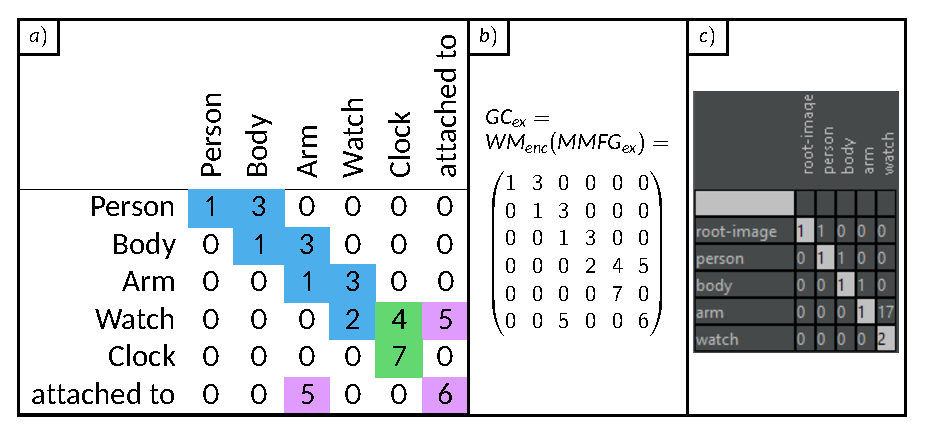
\includegraphics[width=\textwidth, keepaspectratio]{chapter/chapter_2/valuation-matrix-enc.eps}
    \caption{Codierte Wertungsmatrix bzw. Graph Code $GC_{ex}$ zum entsprechenden Beispiel $MMFG_{ex}$in a) Tabellenform und b) in Form einer Matrix. c) Vom GMAF generierte Graph Code $GC_{ex}$.}
    \label{sec2:sota:subsec:fz-explainablity:fig:mmfg-valuation-matrix-enc}
\end{figure}

%\begin{figure}[htb]
    \centering
    \resizebox{0.8\textwidth}{!}{
        \begin{tikzpicture}

            \definecolor{nodeblue}{RGB}{76, 174, 234}
            \definecolor{syngreen}{RGB}{100, 216, 112}
            \definecolor{comprel}{RGB}{224, 155, 254}
            
            \node (tabl) {
                \begin{tabular}{rcccccc}
                     &  \begin{turn}{90}Person\end{turn}& \begin{turn}{90}Body\end{turn} & \begin{turn}{90}Arm\end{turn} & \begin{turn}{90}Watch\end{turn} & \begin{turn}{90}Clock\end{turn} & \begin{turn}{90}attached to $~$\end{turn} \\ \hline
                    Person      & \cellcolor{nodeblue}1 & \cellcolor{nodeblue}3 & 0 & 0 & 0 & 0 \\ 
                    Body        & 0 & \cellcolor{nodeblue}1 & \cellcolor{nodeblue}3 & 0 & 0 & 0 \\
                    Arm         & 0 & 0 & \cellcolor{nodeblue}1 & \cellcolor{nodeblue}3 & 0 & 0 \\ 
                    Watch       & 0 & 0 & 0 & \cellcolor{nodeblue}2 & \cellcolor{syngreen}4 & \cellcolor{comprel}5 \\ 
                    Clock       & 0 & 0 & 0 & 0 & \cellcolor{syngreen}7 & 0 \\ 
                    attached to & 0 & 0 & \cellcolor{comprel}5 & 0 & 0 & \cellcolor{comprel}6
                \end{tabular}
            };

            \node[anchor=south west, right=1cm of tabl.east] (wm) {
                \shortstack[l]{
                    $GC_{ex} = $ \\
                    $WM_{enc}(MMFG_{ex}) = $\\
                    \vspace*{1.5mm} \\
                    $\begin{pmatrix}
                    1 & 3 & 0 & 0 & 0 & 0  \\
                    0 & 1 & 3 & 0 & 0 & 0  \\
                    0 & 0 & 1 & 3 & 0 & 0  \\
                    0 & 0 & 0 & 2 & 4 & 5  \\
                    0 & 0 & 0 & 0 & 7 & 0  \\
                    0 & 0 & 5 & 0 & 0 & 6  \\
                    \end{pmatrix}$
                }
            };
        \end{tikzpicture}
    }
    \caption{Codierte Wertungsmatrix bzw. Graph Code $GC_{ex}$ zum entsprechenden Beispiel $MMFG_{ex}$.}
    \label{sec2:sota:subsec:fz-explainablity:fig:mmfg-valuation-matrix-enc}
\end{figure}

%\begin{figure}[htb]
%    \centering
%    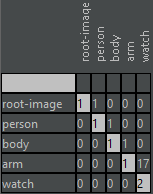
\includegraphics{chapter/chapter_2/gc-ex1.png}
%    \caption{Vom GMAF generierter Graph Code $GC_{ex}$ des Beispiels $MMFG_{ex}$.}
%    \label{sec2:sota:subsec:fz-explainablity:fig:gmaf-gc-ex1}
%\end{figure}

Bei der Berechnung der Ähnlichkeit von Graph Codes müssen diese miteinander verglichen werden.
Damit Graph Codes verglichen werden können, muss der Vergleich dieser Graph Codes auf einer genaustens definierten Metrik für Ähnlichkeit beruhen.
Diese Metrik muss die mathematischen Aspekte eines Vergleichs von Matrizen und auch die semantischen Aspekte von Graph Codes berücksichtigen \cite{gc-2d-proj-mmfg}.
Im nächsten \cref{sec2:sota:par:gc-vocabulary-dictionary} werden weitere grundlegende Definitionen eingeführt und definiert, die zur Definition einer Metrik zur Ähnlichkeit von Graph Codes notwendig sind und eine Berechnung der Ähnlichkeit von Graph Codes unabhängig von den Typen der Knoten und Kanten ermöglicht.

\paragraph{Vokabular und Wörterbuch eines Graph Codes}
\label{sec2:sota:par:gc-vocabulary-dictionary}
Die Menge der Knoten $V$ in einem MMFG, welche die identifizierten Merkmale darstellen, können als eindeutige Bezeichner für das Vokabular bzw. die Gesamtheit aller Wörter, welche einen MMFG ausmachen, betrachtet werden.
Die Menge dieser Bezeichner wird mit $FVT_{MMFG}=\{fvt_1,...,fvt_n\}$ notiert und stellt somit die Elemente des \enquote{Wörterbuchs} eines Graph Codes dar.
Damit ein Bezeichner $fvt_i$ eines Eintrages in einem Graph Code eindeutig identifiziert werden kann, wird ein Vektor $dict_{GC}$ definiert.
Dieser Vektor bietet eine geordnete Reihenfolge für die Menge an Bezeichner $FVT_{MMFG}$ und weist jedem Bezeichner eine eindeutig definierte Position zu.
Die Ordnung dieser Bezeichner im Vektor $dict_{GC}$ kann durch eine beliebige Strategie, wie z.B. durch Breitensuche, Tiefensuche oder manuell, erfolgen.
Durch den Vektor $dict_{GC}$ kann jedes Feld in der Diagonalen des entsprechenden Graph Codes einem Eintrag im Wörterbuch, dargestellt durch $dict_{GC} = (fvt_1,...,fvt_n)$, zugeordnet werden \cite{gc-2d-proj-mmfg}.
Angewandt auf den Graph Code $GC_{ex}$ ergibt sich für die Menge an Bezeichnern $FVT_{ex}=\{Person,Body,Arm,Watch,Clock,attached~to\}$, sowie der Vektor $dict_{ex}=(Person,Body,Arm,Watch,Clock,attached~to)$.
Die Reihenfolge der Bezeichner in $FVT_{ex}$ ist unerheblich und ist für gewöhnlich zufällig.

Anders als $FVT_{ex}$ weist $dict_{ex}$ eine spezifische Reihenfolge auf, die in \cref{sec2:sota:par:gc-vocabulary-dictionary:tab:dict-ex} dargestellt wird.

\begin{table}[htb]
    \centering
    \begin{tabular}{c|c|c|c|c|c|c}
         Index $i$ & 1 & 2 & 3 & 4 & 5 & 6 \\ \hline
         $fvt_i$ & Person & Body & Arm & Watch & Clock & attached to 
    \end{tabular}
    \caption{$dict_{ex}$ vom Graph Code $GC_{ex}$.}
    \label{sec2:sota:par:gc-vocabulary-dictionary:tab:dict-ex}
\end{table}

Beim Vergleichen von Graph Codes ist es wichtig nur die Einträge äquivalenter Merkmale in den Diagonalen der Graph Codes miteinander zu vergleichen.
Da jeder Graph Code einen individuellen Vektor $dict_{GC}$ mit individueller Ordnung besitzt, unterscheiden sich die Wörterbücher der Graph Codes für gewöhnlich voneinander $dict_{GC_1} \neq dict_{GC_2}$.
Äquivalente Merkmale können durch die Schnittmenge der Bezeichner bestimmt werden: $FVT_{1 \cap 2} = \{fvt_1,...,fvt_n\} = V_{MMFG_1} \cap V_{MMFG_2}$.
Analog kann dieses Prinzip auch auf die Wörterbücher von Graph Codes angewendet werden: $dict_{1 \cap 2 } = dict_{GC_1} \cap dict_{GC_2}$.
Aufgrund der unterschiedlichen Ordnungen der Wörterbücher von Graph Codes können diese nicht einfach miteinander verglichen werden, da die Einträge in den zu vergleichenden Graph Codes unterschiedliche Bezeichner darstellen.
Um diesem Problem zu begegnen und die Ordnung von Graph Codes anzupassen, gibt es eine Äquivalenzfunktion $f_{equ}(M_{\cap})$, die die Matrix der Schnittmenge der Wertematrizen bzw. das Wörterbuch so transformiert, dass das entsprechende Wörterbuch nach dem Vektor bzw. Wörterbuch $dict_{\cup}$ geordnet ist \cite{gc-2d-proj-mmfg}.

Konträr zur Schnittmenge kann auch eine Vereinigung von Graph Codes erfolgen.
Eine Vereinigung kann dann erfolgen, wenn eine Applikation eine Sammlung an MMFGs enthält.
Im Falle der Vereinigung von Graph Codes werden die Menge der Bezeichner, sowie die Wörterbücher der Graph Codes miteinander vereint.
Die Gesamtheit aller Bezeichner $FVT_{Coll}$ kann als Vereinigung aller Bezeichner in der Sammlung an MMFGs definiert werden und als Vereinigung aller Wörterbücher dargestellt werden $dict_{\cup}: FVT_{Coll} = \bigcup^{n}_{i=1} FVT_{MMFG_i}$ mit $\forall i,j < n: dict_{\cup} = dict_i \times dict_j$.
Um die Vereinigung der Wörterbücher zu erstellen, wird jedes Wörterbuch $dict_i$ durchlaufen und, sofern noch nicht im Wörterbuch $dict_{\cup}$ vorhanden, jeder individueller Bezeichner hinzugefügt.
Wird ein $dict_{\cup}$ aus der vollständigen Sammlung an Graph Codes berechnet, so kann $dict_{\cup}$ als ein globales Wörterbuch betrachtet werden, in welchem jeder einzigartige Bezeichner eine einzigartige Position besitzt \cite{gc-2d-proj-mmfg}.

%Im folgenden Abschnitt wird anhand der in diesem Abschnitt eingeführten Definitionen eine Metrik zur Ähnlichkeit von Graph Codes vorgestellt und beschrieben.

% Die in diesem Abschnitt beschriebenen Definitionen ermöglichen eine effiziente und effektive Verarbeitung von Informationen von Graph Codes...
% Im nächsten Abschnitt wird solch eine Verarbeitung, die Berechnung der Ähnlichkeit zweier Graph Codes beschrieben.
% Die Berechnung ist ein gutes Beispiel, da es in unterschiedlichsten Anwendungsfällen, wie der Bestimmung der Gemeinsamkeiten oder Unterschiede Verwendung finden kann.

Die in diesem Abschnitt beschriebenen Definitionen ermöglichen eine effiziente und effektive Verarbeitung von Informationen eines Graph Codes.
Ein Beispiel für so eine Verarbeitung ist die Berechnung der Ähnlichkeit zweier Graph Codes, die auf einem Vergleich dieser beiden basiert.
Wie bereits erwähnt, muss der Vergleich dieser Graph Codes auf einer genaustens definierten Metrik beruhen.
%Mit Hilfe dieser Metriken können Eigenschaften von Graph Codes quantifiziert werden und 
Im nächsten Abschnitt werden diese Metriken vorgestellt.

\paragraph{Ähnlichkeit von Graph Codes}
\label{sec2:sota:par:gc-similiarity}
In diesem Abschnitt wird eine Metrik zur Berechnung der Ähnlichkeit bzw. zum Vergleich von Graph Codes beschrieben.
Die in diesem Abschnitt vorgestellten Metriken wurden aus \cite{gc-2d-proj-mmfg} entnommen und ermöglichen die Quantifizierung der Eigenschaften von Graph Codes.
Diese Metrik muss die Zeilen, Spalten und die Einträge, die die Knoten und Kanten darstellen, berücksichtigen.
D.h. diese Metrik zur Berechnung der Ähnlichkeit von Graph Codes muss auf Matrizen anwendbar sein, dessen Zeilen und Spalten die Knoten und Kanten eines MMFGs darstellen.
Damit ein Vergleich dieser Einträge möglich ist, müssen die Einträge vom selben Typ sein.
Da die Wörterbücher von Graph Codes für gewöhnlich unterschiedlich sind, ist es zudem wichtig die korrekten Einträge in einer Matrix zu vergleichen \cite{gc-2d-proj-mmfg}.
Es kann zwischen drei Typen an Einträgen differenziert werden:
\begin{itemize}
    \item Knoten (stellt Merkmale dar)
    \item Kanten (Beziehungen zwischen Knoten bzw. Merkmalen)
    \item Kantentyp (Typ der Beziehung zwischen Knoten bzw. Merkmalen)
\end{itemize}
Für jeden Typ eines Eintrages kann jeweils eine eigene Metrik definiert werden:
\begin{itemize}
    \item Metrik für Merkmale $M_F$
    \item Metrik für Merkmalsbeziehungen $M_{FR}$
    \item Metrik für Beziehungstypen $M_{RT}$
\end{itemize}
Diese Metriken können wiederum als Tripel in einer Metrik $M_{GC} = (M_F, M_{FR}, M_{RT})$ zusammengefasst werden und bilden die gesamte Metrik, die die Ähnlichkeit von Graph Codes darstellen soll.
Diese Metriken werden im Folgenden vorgestellt und beschrieben.

% Metriken eindampfen
% Was ist die Aufgabe einer Metrik?
% Was zeichnet diese Metrik aus?
% Anwendungsbeispiel bzw. fall einer Metrik?
% Nochmal über den technischen Aspekt nachdenken...

Die \textbf{Metrik für Merkmale} $M_F$ berechnet die Ähnlichkeit von Graph Codes anhand der Schnittmenge der Bezeichner in einem Wörterbuch.
Die Metrik $M_F$ ist definiert als das Verhältnis zwischen der Kardinalität der Schnittmenge von Bezeichnern $dict_{\cap}$ der Wörterbücher $dict_i$ und $dict_j$ der Graph Codes $GC_i$ und $GC_j$ und der Kardinalität des Wörterbuchs $dict_i$ vom Graph Code $GC_i$.
Die Formel für diese Metrik lautet $M_F(GC_i, GC_j) = \frac{\abs{dict_{\cap}}}{\abs{dict_i}}$.
Hierbei bezeichnet $\abs{\Vec{v}}$ die Kardinalität eines Vektors, sprich die Anzahl der Elemente in einem Vektor.
Anders formuliert, ist der Wert der Ähnlichkeit höher, desto mehr Merkmale zwei Graph Codes gemeinsam haben.
Es ist wichtig anzumerken, dass diese Metrik nur Knoten bzw. Merkmale betrachtet, unabhängig von den Beziehungen zwischen diesen Merkmalen \cite{gc-2d-proj-mmfg}.

Die \textbf{Metrik für Merkmalsbeziehungen} $M_{FR}$ ist die Grudlage für die Berechnung der Ähnlichkeit von Beziehungen zwischen Merkmalen.
Beziehungen in einem Graph Code werden durch Einträge dargestellt, die nicht in der Diagonalen der Matrix vorkommen und deren Wert größer null ist.
Dabei bezieht die Berechnung dieser Metrik nur Einträge aus der Schnittmenge $M_{\cap}$ der Matrizen ein, die Beziehungen mit demselben Ausgang- und Zielknoten darstellen.
Die Berechnung dieser Metrik basiert auf den nicht in der Diagonalen vorkommenden Einträgen der Adjanzenzmatrix $AM(M_{\cap})$.
Die Metrik $M_{FR}$ ist definiert als das Verhältnis zwischen der Summe aller nicht in der Diagonalen vorkommenden Einträge und der Kardinalität aller nicht in der Diagonalen vorkommenden Einträge.
Die Formel für diese Metrik lautet $M_{FR}(GC_i, GC_j) = \frac{\Sigma AM(M_{i~\cap~j}) -n}{\abs{AM(M_{\cap~i})} - n}$.
Die Metrik $M_{FR}$ stellt somit das Verhältnis zwischen der Zahl der Einträge, die Beziehungen darstellen und der Anzahl der äquivalenten und in der Schnittmenge vorkommenden Einträge, die Beziehungen darstellen, von Graph Codes.
Somit zählt die Metrik $M_{FR}$ die Anzahl aller Beziehungen zwischen Ausgangs- und Zielknoten. 
Die Metrik berücksichtigt jedoch nicht die Äquivalenz der Typen der Beziehungen.
Die Äquivalenz der Typen von Beziehungen wird von der nächsten Metrik, der Metrik für Beziehungstypen berücksichtigt \cite{gc-2d-proj-mmfg}.

Die \textbf{Metrik für Beziehungstypen} $M_{RT}$ basiert auf der Metrik für Merkmalsbeziehungen.
Die Codierungsfunktion $f_{enc}$ codiert für verschiedene Typen von Beziehungen unterschiedliche Werte.
Eine Ähnlichkeit von Typen von Beziehungen setzt aber voraus, dass die Einträge, die die Beziehungen darstellen, vom selben Typ sind, damit sie verglichen werden können.
Diese Metrik führt die Berechnungen nicht mehr anhand der Adjanzenzmatrix der zu vergleichenden Graph Codes aus, sondern anhand der Schnittmenge $M_{\cap}$ der codierten Wertungsmatrizen.
Bei dieser Berechnung wird die Subtraktion auf äquivalenten Einträgen der zu vergleichenden Graph Codes durchgeführt.
Ist das Ergebnis dieser Subtraktion gleich null, so ist der Typ der Beziehung äquivalent.
Sind alle äquivalenten Einträge gleich, so ist die Summe der Subtraktionen dieser Einträge zueinander gleich null.
Im Vergleich zur Metrik $M_{FR}$, die nur Berechnungen anhand einer Adjanzenzmatrix durchführt, verwendet diese Metrik zusätzlich den Wert der Codierung, welche den Typ der Beziehung darstellt, um festzustellen, ob die verglichenen Typen äquivalent sind.
Die Metrik $M_{RT}$ ist definiert als das Verhältnis zwischen der Summe aller nicht in der Diagonalen vorkommenden Einträge und der Kardinalität dieser Einträge.
Die Formel für diese Metrik lautet $M_{RT}(GC_i,GC_j) = \frac{\Sigma^{n,i \neq j}_{i,j}(\abs{M_{\cap i} - M_{\cap j}})}{\abs{M_{\cap i} - n}}$ \cite{gc-2d-proj-mmfg}.

\paragraph{Erklärbarkeit von Graph Codes}
Analog zur Erklärbarkeit von MMFGs in \cref{sec2:sota:par:explainability-of-mmfgs}, muss die technische Darstellung der Merkmale in eine für Menschen verständliche Bedeutung überführt werden.
Auch hier gilt es in einem ersten Schritt die Lücke zwischen der technischen Darstellung und ihrer semantischen Darstellung zu überbrücken.
Die semantische Darstellung von Merkmalen wurde in \cref{sec2:sota:par:explainability-of-mmfgs} bereits durch das Anbinden von externen Informationssystemen erreicht und resultierte in SMMFGs.
Das Anwenden der Algorithmen von Graph Codes auf SMMFGs ermöglicht die semantische Darstellung von Merkmalen in Graph Codes und führt zu Sementischen Graph Codes (SGCs) \cite{towards_auto_sem_expl_mmfg}.
Während das Wörterbuch eines Graph Codes die Menge der Bezeichner der Merkmale darstellt, stellt das Wörterbuch eines Semantischen Graph Codes die semantische Darstellung der Bedeutung dieser Bezeichner dar.
Analog zu MMFGs können auch für Graph Codes, durch das Definieren und Anwenden einer formalen kontextfreien Phrasenstruktur-Grammatik in Kombination mit Semantischen Graph Codes, für Menschen lesbare, verständliche und auf natürlicher Sprache basierende Ausdrücke generiert werden.
Die Erweiterung von Graph Codes um eine formale kontextfreie Grammatik führt zu Erklärbaren Semantischen Graph Codes (ESGCs) \cite{exp-mmfg}.

In Bezug auf Graph Codes ist wichtig anzumerken, dass Graph Codes nicht einen allgemeinen Ersatz bzw. eine allgemeine Alternative zu MMFGs darstellen und nur in bestimmten Fällen, wie z.B. beim Vergleich von MMFGs zur Bestimmung der Ähnlichkeit, eine Verbesserung bieten \cite{gc-2d-proj-mmfg}.
Des Weiteren werden Erklärungen von Graph Codes bislang nur anhand statistischer und rein mathematischer Vorangehensweisen erzeugt.
Es existiert keine Möglichkeit oder Untersuchung Systeme generativer KI zur Erklärbarkeit von Graph Codes zu nutzen.
Dies führt zur ersten offenen Herausforderung.

\begin{tcolorbox}[minipage, colback=white, colframe=black, arc=0pt, outer arc=0pt]
    \textbf{Offene Herausforderung OH 1.1 - Erklärbarkeit durch generative KI} \\
    Einsatz von generativer KI als Ersatz bzw. Alternative zur statistischen und rein mathematischen Vorgehensweise um Erklärungen zu generieren.
\end{tcolorbox}
Die offene Herausforderung \textbf{OH 1.1} wird im Rahmen einer Modellierung, sowie Implementierung in jeweils \hyperref[sec3:model:subsec:fz-explainability]{FZ 1.2/TB} und \hyperref[sec4:impl:subsec:fz-explainability]{FZ 1.3/I} angesprochen und untersucht.

\subsubsection{Generative KI}
\label{sec2:sota:subsubsec:genai}
Generative künstliche Intelligenz (GenKI, engl. generative AI (GenAI)) ist ein Typ künstlicher Intelligenz, die es ermöglicht, anhand vorhandener Informationen und Vorgaben, eine große Vielfalt an neuen Inhalten zu erstellen.
Beispiele für diese Inhalte können Bilder, Videos, Audiodateien, Texte oder anderweitige synthetische Daten sein \cite{gen-ai-tech-target}.
Synthetische Daten bezeichnet Daten, die nicht auf natürliche, sondern auf künstliche Art und Weise durch eine KI erstellt wurden, um echte Daten zu erweitern, oder zu ersetzen \cite{synt-data-ibm}.
Damit eine generative KI synthetische Daten erzeugen kann, wird das Modell der KI mit Hilfe eines Algorithmus anhand echter Daten so trainiert, dass es in der Lage ist, die ursprüngliche Struktur und die Eigenschaften, wie Muster, Zusammenhänge und statistische Merkmale, der echten Daten zu reproduzieren \cite{synth-data-eu, synth-mostlyai}.
Generative KI wird daher als generativ bezeichnet, da sie auf Grundlage bereits vorhandener Datensätze etwas Neues bzw. etwas bisher nicht Dagewesenes erzeugt.
Diese Eigenschaft hebt generative KI wesentlich von diskriminativer KI ab, welche einzig und allein zwischen verschiedenen Eingaben differenzieren kann \cite{computer-woche-genai}.

Ein Anwendungsbeispiel für eine diskriminative KI wäre eine simple binäre Klassifikation von Bildern und ob ein Bild eine Katze darstellt bzw. enthält, oder nicht.
Mit genügend Daten kann das diskriminative Modell einer KI so trainiert werden, dass es bestimmte Eigenschaften, wie Formen und Texturen, die einer Katze gleichen, in einem Bild erkennen kann.
Anhand erkannter Merkmale kann das Modell eine Vorhersage treffen, ob in einem Bild eine Katze zu sehen ist, oder nicht.
Eine wichtige Voraussetzung für das Training dieses Modells ist es, dass jede Beobachtung in den Trainingsdaten manuell mit einer Bezeichnung versehen ist.
Im Fall einer binären Klassifikation sind die Bilder, die Katzen darstellen bzw. enthalten, mit der Bezeichnung 1 versehen, alle anderen Bilder mit der Bezeichnung 0.
Durch das Training erlernt das diskriminative Modell beide Gruppen zu unterscheiden.

Die diskriminative Modellierung ist daher gleichbedeutend mit dem überwachten maschinellen Lernen (engl. supervised machine learning) \cite{orlly-deep-gen-learning}.
In der Tat wird ein Großteil der diskriminativen Modelle für überwachtes maschinelles Lernen verwendet \cite{turing-genai}.
Diskriminative KI bildet also die Eingabe eines mit Bezeichnungen versehenen Datensatzes auf eine Ausgabe ab.
Im Vergleich dazu benötigt das Training eines generativen Modells für gewöhnlich keine explizit mit Bezeichnungen versehenen Datensätze und kann somit mit dem nicht überwachten maschinellen Lernen (engl. unsupervised machine learning) gleichgesetzt werden. 
Das Training auf einem mit Bezeichnungen versehenen Datensatz ist damit allerdings nicht ausgeschlossen und kann auch Verwendung finden \cite{orlly-deep-gen-learning}.

Es ist wichtig anzumerken, dass generative KI, die auf der Methode des Deep Learnings aufbaut, nicht neu ist und bereits in den 60ern in Form von Chatbots vorgestellt wurde \cite{gen-ai-tech-target}.
Die erste Instanz eines solchen Chatbots hieß \enquote{ELIZA} \cite{eliza} und wurde 1966 am MIT entwickelt und hatte zur Aufgabe Gespräche mit einem Pyschotherapeuten zu simulieren \cite{computer-woche-genai}.
Durch das Aufkommen von künstlichen neuronalen Netzwerken (engl. articial neural networks (ANN)) und entsprechender Algorithmen in den 80ern und 90ern, sowie durch bessere Datenlage und Rechenkapazitäten wurde die Methode des Deep Learning praxistauglicher.
Die in 2014 von Ian Goodfellow vorgestellte Technik der generativen gegnerischen Netzwerke (engl. generative adversarial networks (GAN)) führte zu einem Durchbruch und ermöglichte es generativer KI überzeugend wirkende neuartige Inhalte zu generieren \cite{medium-genai-history}.

\paragraph{Grundlegende Techniken und Konzepte}
\label{sec2:sota:par:basic-concepts}
In diesem Abschnitt wird genauer auf wichtige Techniken und Technologien eingegangen, die in aktuellen generativen KI-Systemen Verwendung finden.
Die Techniken und Technologien werden kurz beschrieben und erläutert.
Zuerst werden die allgemeinen Techniken, wie Machine Learning oder Deep Learning vorgestellt bzw. rekapituliert und weiter wichtige Konzepte im Bereich der generativen KI angesprochen.
Die in diesem Abschnitt vorgestellten Techniken bzw. Technologien sind dabei so geordnet, dass sie einer logischen Abfolge in Bezug auf ihre Abhängigkeiten zueinander folgen.

\textbf{Machine Learning} (z.Dt. maschinelles Lernen) ist ein Teilbereich der KI \cite{machine-learning-big-data-insider} und hat zum Ziel die Art und Weise, wie Menschen lernen zu imitieren \cite{ai-ml-dl}.
Maschinelles Lernen ermöglicht es Systemen, Muster und Zusammenhänge automatisch und selbstständig aus Daten und Erfahrungen zu erlernen und zu verbessern, ohne dabei explizit programmiert zu sein \cite{machine-learning-data-absolut}.
Damit Machine Learning funktioniert und Muster und Zusammenhänge erlernt werden können, muss ein Datensatz zum Training vorhanden sein \cite{machine-learning-data-absolut}.
Im Bereich der KI spielen \textbf{(un)-supervised machine learning} (z.Dt. (un)-überwachtes maschinelles Lernen) eine zentrale Rolle \cite{machine-learning-big-data-insider}.
Überwachtes Lernen zeichnet sich dadurch aus, dass Algorithmen mit Hilfe von Daten trainiert werden, die im Trainingsdatensatz manuell mit Bezeichnungen versehen wurden \cite{machine-learning-data-absolut}.
Daher ist überwachtes Lernen mit einem relativ hohen menschlichen Aufwand verbunden \cite{machine-learning-data-absolut}.
Weit verbreitete Problemstellungen bzw. Aufgaben, in denen überwachtes Lernen eingesetzt werden, sind die Klassifikation und Regression \cite{machine-learning-algorithms-quick-review}.
Unüberwachtes Lernen zeichnet sich hingegen dadurch aus, dass es ohne die Einflussnahme von Menschen Gemeinsamkeiten, Unterschiede, Gruppen und Muster in Daten erkennen kann \cite{machine-learning-data-absolut}.
Unüberwachtes Lernen hat, aufgrund seiner Fähigkeit Muster eigenständig erlernen zu können, viele Anwendungsfälle und kann besonders für die Bildanalyse, wie Objekterkennung, oder für die Erkennung von Auffälligkeiten in Daten Verwendung finden \cite{machine-learning-ibm}.

\textbf{Deep Learning} (z.Dt. tiefes Lernen) ist eine besondere Form des maschinellen Lernens und ist in der Lage große Datenmengen zu verarbeiten \cite{deep-learning-ibm}.
Im Mittelpunkt des tiefen Lernens stehen \textbf{Articial Neural Networks (ANNs)} (z.Dt. künstliche neurale Netzwerke (KNN)), die ebenfalls ein Teilgebiet des maschinellen Lernens sind \cite{ibm-ai-ml-dl}.
Künstliche neuronale Netzwerke sind Algorithmen, deren Struktur und Verhalten nach dem biologischen Vorbild des menschlichen Gehirns und seiner Neuronen modelliert ist \cite{deep-learning-ibm,deep-learning-data-absolut}.
%Diese Netzwerke ermöglichen es Modellen tiefen Lernens komplexe Merkmale zu extrahieren und genaue Vorhersagen zu treffen.
Neuronale Netzwerke ermöglichen somit das Erlernen von komplexen Mustern und sind in der Lage genaue Vorhersagen zu treffen.
Da tiefes Lernen sehr rechenintensiv ist, kann es Monate dauern, bis Vorhersagen und Entscheidungen gute Ergebnisse liefern \cite{deep-learning-data-absolut}.
Ein sehr bekanntes Beispiel für ein neuronales Netzwerk ist der Suchalgorithmus von Google \cite{ibm-ai-ml-dl}.
Bekannte Modelle tiefen Lernens im Bereich der generativen KI sind \textbf{Generative Adverserial Networks (GANs)} \cite{goodfellow-gan} und \textbf{Variational Auto Encoders (VAEs)} \cite{kigma-vaes}.

%\textbf{Large Language Models (LLMs)} (z.Dt. großes Sprachmodell) sind große generative Sprachmodelle und stellen ein Teilbereich der KI dar.
%Die Architektur von LLMs basiert auf neuronalen Netzwerken, spezifischer \textbf{Transformern}.
%LLMs sind auf natürlicher Sprache trainiert und sind spezialisiert auf die Verarbeitung von natürlicher Sprache (NLP).
%D.h. LLMs sind in der Lage natürliche Sprache zu verstehen, zu verarbeiten und Ausdrücke natürlicher Sprache zu generieren.
%LLMs werden auf riesigen Textmengen trainiert und weisen in der Praxis Milliarden an Parameter auf.
%LLMs arbeiten mit Statistik und Wahrscheinlichkeitsverteilungen und optimieren mit diesen die Genauigkeit ihrer Vorhersage für die wahrscheinlichste Komplementierung des Textes \cite{towards-data-science-icl}.

\textbf{Large Language Models (LLMs)} (z.Dt. großes Sprachmodell) sind große generative Sprachmodelle und stellen einen Teilbereich der KI dar \cite{nvidia-llm}.
Eine sehr prominente Architektur von großen Sprachmodellen sind Transformer \cite{nvidia-llm}.
Die Architektur von Transformern basiert auf neuronalen Netzwerken und zeichnet sich dadurch aus, dass es Kontext und Bedeutung durch Beobachtung der Beziehungen zwischen Wörtern erlernen kann \cite{nvidia-llm}.
Transformer wurden zuerst von Google in \enquote{Attention Is All You Need.} \cite{google-attention} vorgestellt und führen zwei neue Techniken ein: positionelle Kodierung und Selbstaufmerksamkeit \cite{nvidia-llm}.
Große Sprachmodelle werden meist durch unüberwachtes Lernen auf riesigen Datenmengen trainiert und weisen in der Praxis Milliarden an Parameter auf \cite{nvidia-llm}.
Als solches erlernen LLMs die Muster der Statistiken und Wahrscheinlichkeitsverteilungen innerhalb der Trainingsdaten und optimieren mit diesen die Genauigkeit ihrer Vorhersagen anhand ihrer Anwendungsfälle \cite{towards-data-science-icl}.
Anwendungsfälle von Transformern sind vielfältig und können das z.B. Erzeugen, Übersetzen oder Zusammenfassen von Text umfassen \cite{nvidia-llm}.

\textbf{Explainable AI (xAI)} (z.Dt. erklärbare KI) befasst sich mit der Erklärbarkeit von KI.
Erklärbare KI beschäftigt sich u.a. mit der Frage \enquote{Wie kommt eine KI zu einem Ergebnis} und versucht die inneren Abläufe in einer KI zu beleuchten \cite{explainable-ai-kobold}.
Das generelle Problem mit KI ist, dass die Algorithmen wie neuronale Netzwerke und tiefes Lernen sogenannte \enquote{Black-Boxes} sind \cite{explainable-ai-kobold}.
Zwar ist die Funktionsweise dieser Algorithmen, sowie das finale Ergebnis bekannt, aber es ist nicht erkenntlich wie die KI dieses Ergebnis erreicht hat \cite{explainable-ai-kobold}.
Ziel von erklärbarer KI soll also sein, dass ein Mensch nachvollziehen kann, wie ein Algorithmus ein Ergebnis erreicht \cite{explainable-ai-kobold}.

Die meisten Systeme generativer KI arbeiten mit einer sogenannten \textbf{Prompt} (z.Dt. Eingabeaufforderung) als Eingabe.
Im Rahmen der Verarbeitung natürlicher Sprache und des maschinellen Lernens bezeichnet ein Prompt ein Stück Text, das als eine Anweisung an ein System verstanden werden kann und welches den Kontext und alle dazugehörigen und notwendigen Informationen enthält, damit ein Modell relevante Ausgaben erzeugen kann \cite{gradientpub-prompt,hopsworks-prompt-engineering}.
Anwendungsbeispiele für Prompts können Erklärungen, Fragen oder anderweitige Texteingaben sein.
Das Modell eines Systems verarbeitet die Eingabe und produziert in Abhängigkeit der Eingabe und der Fähigkeiten des jeweiligen Modells entsprechende Ausgaben, wie z.B. Vervollständigungen von Text, Erklärungen, Übersetzungen, Zusammenfassungen oder Bilder.
Beim Dirigieren des Verhaltens eines Systems spielen Prompts daher eine entscheidende Rolle \cite{skimai-prompts}.
Grundlegende Elemente oder Inhalte einer Prompt können Anweisungen, Kontext, Eingabedaten oder Angaben zur gewünschten Ausgabe umfassen \cite{promptingguide-basiscs-prompting}.
Bereits durch einfache Prompts können viele Aufgaben ausgeführt werden, jedoch hängt die Qualität der Ausgabe von der Qualität der Eingabe ab \cite{promptingguide-basiscs-prompting}.
Durch das Bereitstellen von mehr Informationen in einer Prompt können die Wahrscheinlichkeiten zum Generieren gewünschter Ausgaben erhöht werden.
Dieser Ansatz, Prompts anzupassen, um optimale Ergebnisse zu erzielen, heißt \textbf{Prompt Engineering} (z.Dt. Entwicklung von Eingabeaufforderungen) \cite{promptingguide}.
Prompt Engineering ist, in Essenz, ein iterativer, experimenteller Prozess.
Begonnen wird zumeist mit einfachen Prompts, die iterativ und inkrementell weiterentwickelt werden.
Einfache Anpassungsmöglichkeiten sind Prompts schlicht, kurz und knapp zu halten und eine möglichst präzise Formulierung zu verwenden.
Diese Anpassungsmöglichkeiten können durch bekannte Techniken des Prompt Engineering, wie Zero-Shot \cite{promptingguide-zero-shot}, Few-Shot \cite{promptingguide-few-shot} und Chain-of-Thought (CoT) \cite{promptingguide-cot} erweitert werden.

\textbf{Zero-Shot} ist eine Technik, in der Modelle wie GPT-3.5 aufgrund der großen Datenmengen, mit welchen sie trainiert wurden, in der Lage sind Prompts ohne vorher spezifizierte Informationen oder Beispiele wirksam auszuführen \cite{promptingguide-zero-shot}.
Ein Anwendungsbeispiel für Zero-Shot Prompting ist die folgende Instruktion einen Text in eine andere Sprache zu übersetzen.

\begin{tcolorbox}[colback=white, top=1pt, bottom=1pt, left=2pt]
    \textbf{Eingabe}: Übersetze \enquote{Das Auto hat einen Platten} in Englisch.
    \tcbline
    \textbf{Ausgabe}: \enquote{The car has a flat tire}.
\end{tcolorbox}

\textbf{Few-Shot} beschreibt eine Technik, die sich dadurch auszeichnet, dass der Prompt Instruktionen in Form von ergänzenden Informationen zum Ausführen der Prompt beigefügt werden \cite{promptingguide-few-shot}.
Ein Anwendungsbeispiel für Few-Shot Prompting ist die folgende Reihe an Prompts, die als Beispiele dienen.

\begin{tcolorbox}[colback=white, top=1pt, bottom=1pt, left=2pt]
    \textbf{Eingabe}: \enquote{Hauptstadt der Niederlande ist ...}. \newline
    \textbf{Ausgabe}: \enquote{Amsterdam}. \newline
    \textbf{Eingabe}: \enquote{Hauptstadt von Norwegen ist ...}. \newline
    \textbf{Ausgabe}: \enquote{Oslo}. \newline
    \textbf{Eingabe}: \enquote{Hauptstadt von Deutschland ist ...}.
    \tcbline
    \textbf{Ausgabe}: \enquote{Berlin}.
\end{tcolorbox}
In diesem Beispiel wird dem Modell eine Reihe an Beispielen für das gewünschte Verhalten bereitgestellt.
Anhand dieser Beispiele soll das Modell das Muster erkennen und erlernen, um ähnliche Fragen beantworten zu können.

\textbf{Chain-of-Thought} hingegen zeichnet sich dadurch aus, dass die Anweisung, die mit einer Prompt vermittelt werden soll, in eine Reihe an Schritten heruntergebrochen wird \cite{google-cot}.
Für jeden Schritt in dieser Reihe wird wiederum ein Prompt definiert.
Ein Anwendungsbeispiel für eine leicht modifizierte Technik von CoT ist die folgende Prompt.

\begin{tcolorbox}[colback=white]
    \textbf{Aussage}: Die ungeraden Zahlen in folgender Zahlenreihe ergeben eine gerade Zahl: 6, 4, 7, 12, 19, 1, 2.
    Gehe schrittweise vor.
    \tcbline
    \textbf{Antwort}:
    \begin{enumerate}
        \item Alle ungeraden Zahlen in der Reihe identifizieren: 7, 19, 1.
        \item Alle ungeraden Zahlen addieren: 7 + 19 + 1 = 27.
        \item Feststellen, dass 27 eine ungerade Zahl ist.
        \item Erkennen, dass die usprüngliche Aussage \enquote{Die ungeraden Zahlen in folgender Zahlenreihe ergeben eine gerade Zahl: [...]} eine falsche Aussage ist.
    \end{enumerate}
\end{tcolorbox}
In einem ersten Schritt werden die gegebenen Informationen betrachtet und aus der gegebenen Zahlenreihe alle ungeraden Zahlen identifiziert.
In einem zweiten Schritt formuliert das Modell eine Gleichung zum Summieren der ungeraden Zahlen.
Subsequent wird die aufgestellte Gleichung gelöst und erkannt, dass die Summe der ungeraden Zahlen wiederum eine ungerade Zahl ist.
Im letzten Schritt wird die ursprüngliche Aussage mit den neu gewonnen Fakten verglichen und es wird erkannt, dass die ursprüngliche Aussage falsch ist.

Das Beispiel endet mit dem Satz \enquote{Gehe schrittweise vor} (engl. Lets think step by step).
Durch diesen Satz wird die Anweisung in der Prompt in eine Reihe an Schritten zerteilt.
Das schrittweise Vorgehen hilft dem Modell das Problem besser zu verstehen und die richtige Antwort zu liefern.
Diese Technik wurde zuerst in \cite{zero-shot-reasoners} beschrieben und wird auch Zero-Shot CoT genannt und kombiniert Zero-Shot und CoT miteinander.
Es ist eine leistungsstarke Technik, die eine nicht zu unterschätzende Wirkung auf Schlussfolgerungen des Modells hat und die zur Verbesserung der Leistung von Modellen bei einer Vielzahl von Aufgaben eingesetzt werden kann.

Prompt Engineering ist ein sich rasant entwickelndes Feld im Bereich der generativen KI und stellt mittlerweile auch einen eigenen Beruf dar.
Da Prompt Engineering ein iterativer und inkrementeller Prozess ist, werden stetig neue Techniken entwickelt, oder alte Techniken in neuer Weise miteinander kombiniert.

\paragraph{Systeme generativer KI}
\label{sec2:sota:par:genai-systems}
Systeme generativer KI haben einen enormen Einfluss auf die Weltwirtschaft \cite{mckinsey-economic-genai}.
So kann, laut Schätzungen, generative KI die Produktivität der weltweiten Wirtschaften erhöhen und, unter Berücksichtigung vieler Anwendungsfälle, pro Jahr einen Mehrwert in Höhe von \$2.6 bis \$4.4 Billionen schaffen \cite{mckinsey-economic-genai}.
Dieser steigende wirtschaftliche Anreiz führt zu einer explosionsartigen und rasanten Entwicklung im Bereich der generativen KI und weltweit zur Entwicklung, Integration und Anwendung generativer KI \cite{mckinsey-economic-genai,statista-forecast-ai-market-size}.
Aus diesem Grund ist eine Aufführung, oder gar eine ausführlichere Liste solcher Systeme im Rahmen dieser Arbeit nicht machbar.
Daher werden in diesem Abschnitt nur ausgewählte Systeme generativer KI vorgestellt und kurz beschrieben.
Die Auflistung dieser Systeme erfolgt nach den Kategorien Image und Text, sowie Audio und Video.

Die Kategorie \textbf{Image} zählt eine Auswahl an Programmen auf, die auf KI basieren und in der Lage sind, aus Ausdrücken natürlicher Sprache, Bilder und Kunst zu erzeugen.
Diese Prozesse der Bilderzeugung nennt man Text2Image (z.Dt. Text zu Bild).
Ein paar der bekanntesten Programme sind:

\begin{itemize}
    \item \textbf{DALL·E 2} \cite{dall-e-2} ist eine von OpenAI \cite{openai} entwickelte KI, die mittels Text To Image realistische Bilder und Kunst schaffen kann.
    \item \textbf{Stable Diffusion} \cite{stable-diffusion} ist eine von StabilityAI \cite{stabilityai} entwickelte KI, die ebenfalls auf Grundlage von Ausdrücken natürlicher Sprache Bilder erzeugen kann.
    Im Vergleich zu DALL·E 2 ist Stable Diffusion eine Open Source Software.
    \item \textbf{Midjourney} \cite{midjourney} ist eine KI, die auf Grundlage einer Textbeschreibung Bilder und Kunst erstellen kann. 
\end{itemize}

Die Kategorie \textbf{Text} zählt eine Auswahl an Programmen auf, die auf KI basieren und anhand von Eingaben eines Nutzers, meist einer sogenannten \enquote{Prompt}, die auf Ausdrücken natürlicher Sprache basieren, wiederum Text zu generieren.

\begin{itemize}
    \item \textbf{OpenAI API} bietet Zugang zu OpenAIs Sprachmodellen, wie GPT-3.5 \cite{openai-gpt-sep-2021} und GPT-4 \cite{openai-gpt-sep-2021}.
    Diese Sprachmodelle sind in der Lage anhand Instruktionen in Form von Ausdrücken natürlicher Sprache eine Reihe an Aufgaben durchzuführen.
    % Quelle zu Vertex AI
    \item \textbf{Google Vertex AI} ist eine Plattform für maschinelles Lernen.
    Die \textbf{Vertex AI API} bietet Zugang zu Googles PaLM 2 \cite{google-palm2-techreport}, einer Familie an Sprachmodellen \cite{google-blog-io-23}.
    Spezialisierungen von PaLM 2 umfassen Med-PaLM für medizinische Anwendungsfälle und Sec-PaLM 2 für sicherheitsbezogene Anwendungsfälle \cite{google-blog-io-23}.
    PaLM 2 treibt generative KI-Funktionen, wie die PaLM API, -Tools, sowie Bard \cite{google-bard}, an \cite{google-blog-io-23}.
\end{itemize}

Im Rahmen dieser Arbeit sind vor allem Systeme zur Text- sowie Bilderzeugung von vorrangigem Interesse.
Generative KI ist allerdings nicht auf Text- oder Bilderzeugung beschränkt, sondern kann auch in anderen Bereichen, wie der Audio- oder Videoerzeugung Verwendung finden.
Diese Systeme können, wie bereits in \cref{sec1:intro:subsec:motivation} beschrieben, einen echten Mehrwert für Benutzer darstellen.
Daher wird im Folgenden noch ein kurzer Überblick über die Kategorien Audio und Video gegeben.

In der Kategorie der Programme zur Audioerzeugung gibt es bekannte Systeme, wie die von Eleven Labs \cite{eleven-labs}, Resemble AI \cite{resemble-ai} oder Bark \cite{bark}.
Anwendungsfälle für diese Systeme können multilinguale Synchronisation, das Klonen von Stimmen, oder die automatische Erzeugung von Untertiteln in Videos sein.
In der Kategorie der Programme zur Videoerzeugung sind bekannte Systeme, wie die von RunwayML \cite{runway-ml}, Synthesia \cite{synthesia} oder Rephrase AI \cite{rephrase-ai}.
Anwendungsfälle für diese Art von Systemen können schnelle Videoerzeugung, Videobearbeitung, vor allem im Bereich Marketing oder Nachrichtensendungen sein.

Die nachfolgende \cref{sec2:sota:subsec:fz-explainablity:fig:generative-ai-landscape} zeigt eine Zusammenfassung und kurze Übersicht über ausgewählte aktuelle Systeme generativer KI zusammen mit ihren entsprechenden Anwendungsmöglichkeiten.
Es ist wichtig zu betonen, dass diese Übersicht keinen Anspruch auf Vollständigkeit erhebt, da sich diese Landschaft rapide verändert und ständig neue Techniken, Technologien und Systeme entwickelt werden.

\begin{figure}[htb]
    \centering
    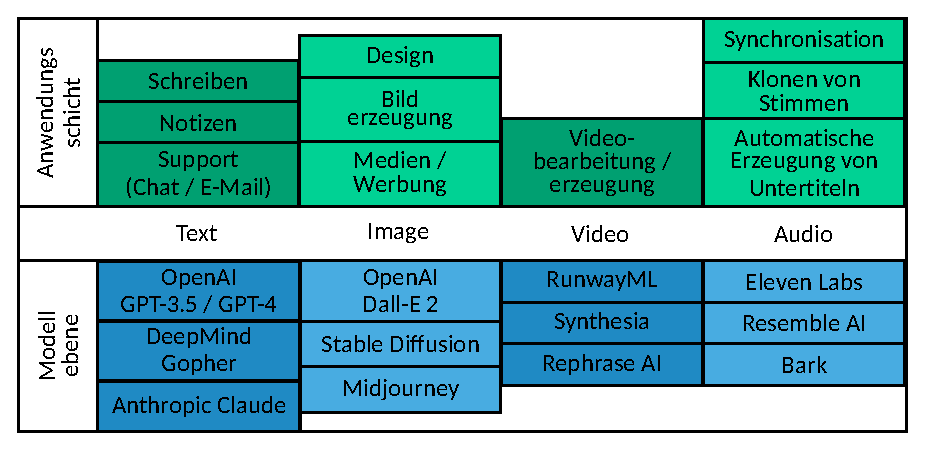
\includegraphics[width=\textwidth]{chapter/chapter_2/generative-ai-landscape.eps}
    \caption{Übersicht ausgewählter aktueller Systeme generativer KI nach \cite{sequoia-genai}.}
    \label{sec2:sota:subsec:fz-explainablity:fig:generative-ai-landscape}
\end{figure}

\FloatBarrier

\paragraph{Einschränkungen}
Systeme generativer KI, wie z.B. das große Sprachmodell GPT-3 von OpenAI, sind bereits in der Lage realistische und höchst überzeugende Inhalte zu erzeugen.
Trotzdem unterliegen Systeme generativer KI einer Reihe an Einschränkungen, die sich potentiell auf ihre Fähigkeiten und Anwendungsfälle auswirken können.
Einige der wichtigsten Einschränkungen von Systemen generativer KI sind:
\begin{enumerate}
    \item \textbf{Mangelnde Transparenz und Erklärbarkeit}: Modelle generativer KI sind sog. Black-Boxen und bieten keinen Einblick in ihren Entscheidungsprozess \cite{explainable-ai-kobold}.
    Aufgrund dieser mangelnder Transparenz ist es nicht ersichtlich, wie ein Modell zu einer Entscheidung und zu einem Ergebnis kommt \cite{explainable-ai-kobold}.
    Resultat ist eine eingeschränkte Erklärbarkeit von Modellen.
    
    \item \textbf{Abhängigkeit von Traingsdaten und ethische Bedenken}: Modelle generativer KI sind Produkte ihrer Trainingsdaten und daher stark von ihnen abhängig \cite{klinkhammer-genai}.
    Aufgrund dieser Abhängigkeit können sich Ungenauigkeiten aus den Trainingsdaten in den generierten Ergebnissen wiederspiegeln \cite{klinkhammer-genai}.
    Des Weiteren sind diese Modelle zumeist speziell auf Bereiche angepasst und lassen sich nur schwer auf andere Bereiche anwenden, die nicht von den Trainingsdaten vorgesehen sind \cite{klinkhammer-genai}.
    Ein weiteres Problem generativer KI sind ethische Bedenken \cite{klinkhammer-genai}.
    Durch Voreingenommenheiten in den Trainingsdaten können Modelle selbst voreingenommene oder gar schädliche Inhalte erzeugen \cite{klinkhammer-genai}.

    %\item \textbf{Mangelndes Verständnis des Kontextes und Mehrdeutigkeit}: Modelle generativer KI haben, trotz Mechanismen, wie z.B. dem Selbstaufmerksamkeitsmechanismus, oft Probleme den Kontext eines Textes zu verstehen \cite{azumo-genai-power}.
    %Sie können deshalb keine komplexen Zusammenhänge erkennen und nachvollziehen.
    %Dies führt aufgrund der Mehrdeutigkeit von natürlicher Sprache zu Problemen in Bezug auf kontextabhängige Aussagen.
    %Generative KI hat Schwierigkeiten, die Mehrdeutigkeiten in einer Aufgabe zu trennen.
    %Dies kann zu ungenauen Ergebnissen mit unbeabsichtigten Bedeutungen führen.

    \item \textbf{Mangelndes Verständnis des Kontextes}: 
    Die Länge des Kontextfensters eines Modells begrenzt die Menge an vorausgehendem Text, welches ein Modell bei der Generierung einer Antwort auf eine Eingabeaufforderung berücksichtigt \cite{v7labs-llm-limitations}.
    Informationen, die außerhalb dieses Kontextfensters liegen, werden unter Umständen nicht mehr berücksichtigt und können zu einem unvollständigen Verständnis des Textes oder zu kontextuell verfälschten Antworten führen \cite{v7labs-llm-limitations}.
    In Kombination mit den ausgewählten Trainingsdaten beeinflusst die Länge des Kontextfensters somit maßgeblich die Fähigkeiten des Modells den Kontext zu verstehen, langfristige Abhängigkeiten zu erfassen und kohärnte Texte zu generieren \cite{v7labs-llm-limitations}.
\end{enumerate}

Trotz der bemerkenswerten Fähigkeit ansprechende und überzeugende Inhalte zu generieren, ist es wichtig die Einschränkungen und Grenzen generativer KI im Blick zu behalten, um so einen effektiven, verantwortungsbewussten und informierten Einsatz von generativer KI garantieren zu können.
Im Bereich der Forschung gibt es laufende Bemühungen und Weiterentwicklungen, um diese Einschränkungen und Grenzen zu adressieren, abzustellen, die Zuverlässigkeit von generativer KI zu verbessern, sowie Fähigkeiten von Systemen generativer KI weiter auszubauen.
Diese Bestrebungen können allgemein unter dem Begriff \enquote{Responsible AI} zusammengefasst werden, welche zum Ziel haben KI auf verantwortungsvolle Art und Weise zu entwickeln und die oben genannten Einschränkungen zu berücksichtigen \cite{gabler-responsible-ai}.

\subsubsection{Diskussion}
\label{sec2:sota:subsubsec:fz1:discussion}
In den ersten {\crefname{subsection}{Abschnitte}{Abschnitten}\cref{sec2:sota:subsubsec:gmaf,sec2:sota:subsubsec:mmfg,sec2:sota:subsubsec:graph-codes}} wurden zuerst grundlegende Technologien in Bezug auf das GMAF, welches das Bezugssystem dieser Arbeit darstellt, vorgestellt und detailliert erläutert.
Weiter wurden in \cref{sec2:sota:subsubsec:genai} grundlegende Techniken und Konzepte im Rahmen der generativen KI genannt und erklärt, sowie aktuelle Systeme generativer KI nach Kategorien gelistet.

Im Rahmen der Diskussion dieses Forschungsziels werden die Anwendungsmöglichkeiten der in \cref{sec2:sota:par:genai-systems} vorgestellten Systeme in Bezug auf das GMAF diskutiert.
Anhand dieser Diskussion wird dann eine fundierte Entscheidung getroffen, welche Systeme generativer KI für die Umgebung \enquote{Erklärbarkeit von MMIR mittels generativer KI} am besten geeignet sind.

Damit eine fundierte und informierte Entscheidung für die Auswahl von Systemen generativer KI getroffen werden kann, gilt es einige Kritieren zur Auswahl von Systemen zu beachten.
Wichtige Kritieren zur Auswahl eines Systems sind:
\begin{itemize}
    \item \textbf{Anpassungsmöglichkeiten}: Wie flexibel ist ein System?
    Ermöglicht es die Anpassung anhand Anforderungen besonderer Anwendungsfälle?
    \item \textbf{Kompatibilität und Integration}: Ist ein System mit der Programmiersprache oder der Umgebung des GMAF kompatibel?
    Bietet das System eine Schnittstelle, um eine einfache Integration des Systems in das GMAF zu ermöglichen?
    Bietet das System eine klare Dokumentation, um die Integration der Schnittstelle zu unterstützen?
    \item \textbf{Skalierbarkeit und Leistung}: Ist das System in der Lage größere Datenmengen zu verarbeiten?
    Kann es auf Anfrage zeitnah Ergebnisse generieren?
    \item \textbf{Kosten und Lizenzierung}: Einige Systeme bieten kostenfreie Nutzung oder berechnen die Kosten abhängig von der Nutzung, wiederum erfordern andere Systeme eine kommerzielle Lizenz zur Nutzung. 
    Welche Lizenzbedingung oder Preise sind mit der Nutzung eines Systeme verbunden?
\end{itemize}

Das Berücksichtigen dieser Kriterien in der Auswahl eines Systems generativer KI ermöglicht eine wohl informierte und fundierte Entscheidung über die Integration eines Systems in das GMAF und legt das Fundament für das Erreichen von Anforderungen und Zielen.
Daher wird zuerst die Auswahl eines Systems aus der Kategorie Image zur Bildgenerierung diskutiert.
Danach folgt eine Diskussion zur Auswahl eines Systems aus der Kategorie Text zur Textgenerierung.
Die Diskussion orientiert sich dabei jeweils nach den Systemen und nicht nach den oben genannten Kriterien.

\paragraph{Ausgewählte Systeme zur Bildgenerierung}
Zur Auswahl eines Systems zur Bildgenerierung stehen OpenAIs DALL·E 2, StabilityAIs Stable Diffusion und Midjourney.
Um einen besseren Eindruck zu den jeweiligen Modellen bzw. Systemen zu ermöglichen, wird für jedes System ein Bild anhand der Textbeschreibung bzw. Prompt \enquote{\textit{Beautiful Venice canals with gondolas and bridges, charming}} generiert.

% Prüfen, ob auch alle Aspekte abgedeckt werden ...
% Beispiele beifügen für die jeweiligen Systeme, um dem Leser besseren Eindruck zu ermöglichen

\textbf{Midjourney} ist eine generative KI, die auf Grundlage einer Textbeschreibung überzeugende und ästhetisch ansprechende Bilder erzeugen kann.
\cref{sec2:sota:subsubsec:fz1:discussion:fig:venice-midjourney} zeigt ein Beispiel für ein von Midjourney generiertes Bild.
\begin{figure}[htb]
    \centering
    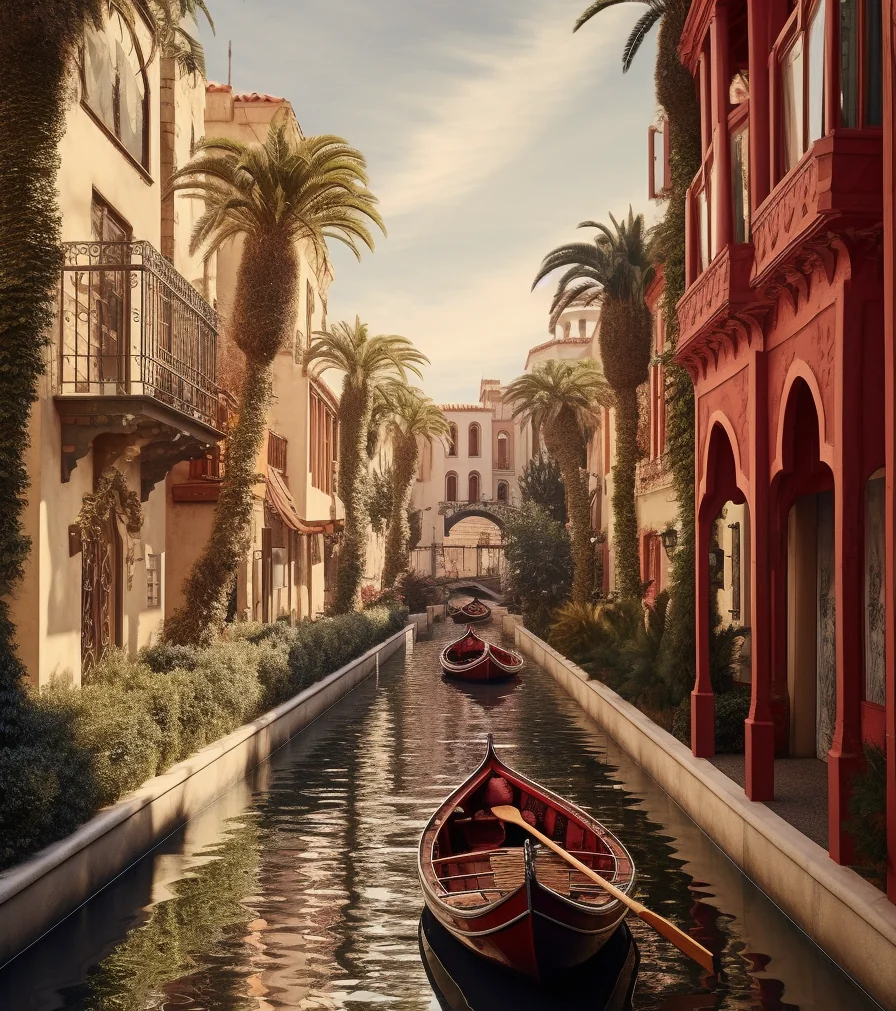
\includegraphics[width=0.65\textwidth, keepaspectratio]{chapter/chapter_2/venice-midjourney.png}
    \caption{Beispiel für ein von Midjourney generiertes Bild anhand oben genannter Textbeschreibung \cite{reddit-venice-midjourney}.}
    \label{sec2:sota:subsubsec:fz1:discussion:fig:venice-midjourney}
\end{figure}
Um auf Midjourney zugreifen zu können, wird eine Anmeldung über den Onlinedienst Discord vorausgesetzt.
Weitere Voraussetzungen zum Nutzen Midjourneys sind das Hinzufügen und Beitreten des Discord-Servers von Midjourney und das Akzeptieren der allgemeinen Nutzungsbedingungen.
Sind diese Voraussetzungen erfüllt, kann Midjourney über Befehle im Discord-Chat gesteuert werden.
Bilder können über den Befehl /imagine und einer Textbeschreibung \textbf{prompt} erzeugt werden.
Midjourney bietet eine Reihe an Anpassungsmöglichkeiten seiner Prozesse, die gezielt durch Befehle, die in \cite{midjourney-docs} dokumentiert sind, vorgenommen werden können.
Midjourney bietet in einem begrenztem Testversuch ein initiales Guthaben von 25 Credits zum Erstellen von Bildern.
Sind diese Credits aufgebraucht, kann aus einer Reihe an unterschiedlichen, gestaffelten Mitgliedschaften (siehe \cite{midjourney-plans}), welche jeweils eigene Vorteile bieten, gewählt werden.
Eine Integration von Midjourney in eine andere Software ist aufgrund einer fehlenden Schnittstelle oder Anbindung bzw. Bibliothek nicht möglich.
Zwar gibt es Drittanbieter, die eine Schnittstelle bereitzustellen scheinen, allerdings verweist Midjourney in seinen allgemeinen Nutzungsbedingungen ausdrücklich, dass es keine Schnittstelle bereitstellt und Automatisierungen nicht duldet \cite{midjourney-tos}.

\textbf{Stable Diffusion} von StabilityAI ist eine quelloffene generative KI, die ebenfalls auf Grundlage einer Textbeschreibung Bilder erzeugen kann.
\cref{sec2:sota:subsubsec:fz1:discussion:fig:venice-stable-diffusion} zeigt ein Beispiel für ein von Stable Diffusion generiertes Bild.
\begin{figure}[htb]
    \centering
    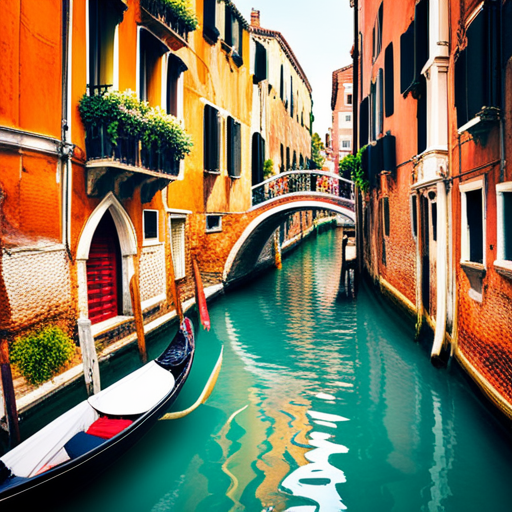
\includegraphics[width=0.65\textwidth, keepaspectratio]{chapter/chapter_2/venice-stable-diffusion.png}
    \caption{Beispiel für ein von Stable Diffusion generiertes Bild anhand oben genannter Textbeschreibung.}
    \label{sec2:sota:subsubsec:fz1:discussion:fig:venice-stable-diffusion}
\end{figure}
Zugriff auf Stable Diffusion kann durch eine Installation auf einer lokalen Maschine oder durch das WebInterface DreamStudio erfolgen.
In beiden Fällen erfolgt der Zugriff durch ein WebInterface, in welchem eine Reihe an Anpassungsmöglichkeiten durch Einstellungen vorgenommen werden können.
%Eine lokale Installation ist im Rahmen dieser Arbeit ausgeschlossen, da für eine vernünftige Nutzung von Stable Diffusion eine Mindestanforderung von 10GB VRAM notwendig ist.
Aufgrund der hohen Rechenanforderungen benötigt eine lokale Installation von Stable Diffusion eine hohe Mindestanforderung an VRAM.
%10GB VRAM mind.
Auch Stable Diffusion bietet in einem begrenztem Testversuch ein initiales Guthaben von 25 Credits.
Sind diese Credits aufgebraucht, können für einen Mindestwert von 10 Euro Credits hinzugekauft werden.
Die Preise für die Generierung von Bildern sind abhängig von den gewählten Eigenschaften der Bilder und können in \cite{sd-pricing} eingesehen werden.
Eigenschaften können die Bildgröße, aber auch die Anzahl der Iterationen der Bildgenerierung sein.
Diese Einstellungen haben einen Einfluss auf die Qualität der generierten Bilder und folglich auch auf die Rechenintensität und beeinflussen dementsprechend die Preise zur Generierung von Bildern.
Eine Integration von Stable Diffusion ist durch eine offizielle REST (Representational State Transfer) \cite{rest} Schnittstelle möglich.
%Stable Diffusion ist lizenziert unter der CreativeML Open RAIL++-M Lizenz.
% Nur anmerken, dass es Schnittstelle gibt, oder noch OpenAPI anmerken?
    
\textbf{DALL·E 2} ist eine generative KI, die ebenfalls auf Grundlage einer Textbeschreibung Bilder erzeugen kann.
\cref{sec2:sota:subsubsec:fz1:discussion:fig:venice-dall·e} zeigt ein Beispiel für ein von DALL·E 2 generiertes Bild.
\begin{figure}[htb]
    \centering
    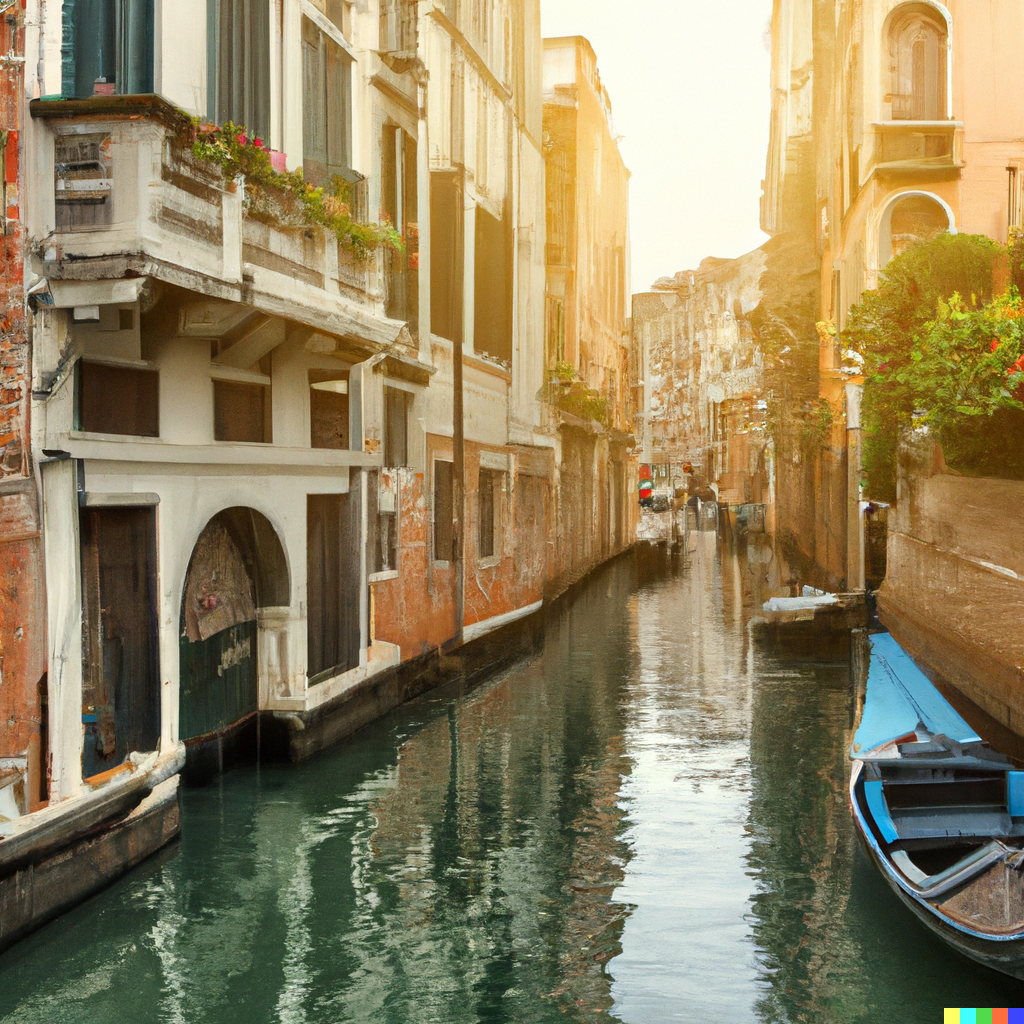
\includegraphics[width=0.65\textwidth]{chapter/chapter_2/venice-dall-e.png}
    \caption{Beispiel für ein von DALL·E 2 generiertes Bild anhand oben genannter Textbeschreibung.}
    \label{sec2:sota:subsubsec:fz1:discussion:fig:venice-dall·e}
\end{figure}
Zugriff auf DALL·E 2 erfolgt über ein WebInterface.
OpenAI bietet monatlich eine freie Anzahl an Credits, mit welchen Bilder erzeugt werden können.
Sind diese Credits aufgebraucht, kann für einen Mindestwert von 15 Dollar 115 Credits hinzugekauft werden.
Im Vergleich zu Stable Diffusion sind die Preise zur Bildgenerierung von DALL·E 2 nur von der Bildgröße abhängig (siehe \cite{openai-pricing}).
OpenAI bietet über eine Schnittstelle Zugriff auf DALL·E 2, sowie andere Modelle.
Diese Schnittstelle verfügt über eine wohl definierte Dokumentation, die in \cite{openai-api-doc} eingesehen werden kann.
Des Weiteren unterstützt OpenAI zur Integration seiner Modelle eine Reihe an Community-Bibliotheken für unterschiedliche Sprachen, darunter eine Anbindung der Schnittstelle für Java (siehe \cite{dall-e-java-api}).
Auch die Dokumentation zur Anbindung der Schnittstelle in Java unterstützt eine klare Dokumentation (siehe \cite{dall-e-java-api}).

Alle drei vorgestellten Systeme ermöglichen das Erzeugen von qualitativ hochwertigen Bildern.
Hinter allen drei Systemen stehen in Bezug auf die Bepreisung der Generation von Bildern sogenannte Credits.
Dabei bieten alle drei Systeme am Anfang eine gewissen Zahl an freien Credits.
Midjourney und Stable Diffusion vergeben beim Erstellen eines Kontos eine endliche Anzahl an Credits.
OpenAI hingegen vergibt ein anfängliches Guthaben von 5 Dollar und monatlich eine freie Anzahl an Credits, die jeden Monat zurückgesetzt werden.
Credits gelten allerdings nicht für die Schnittstelle von OpenAI und werden seperat berechnet \cite{openai-dall-e-seperate-billing}.
Die Anzahl der Credits sind im Rahmen von OpenAI somit nicht von Belang.
Die Berechnung der Preise geschehen im Fall der Schnittstelle von OpenAI nutzungsbasiert und werden am Ende des Monats abgerechnet, anstatt einer monatlichen Zahlung wie im Fall von Midjourney.
Die Tatsache, dass Midjoruney keine Schnittstelle anbietet, disqualifiziert Midjourney für die Auswahl eines Systems zur Bildgenerierung im Rahmen dieser Arbeit.
Offen für die Auswahl bleiben StabilityAIs Stable Diffusion und OpenAIs DALL·E 2.
Ein Argument gegen Stable Diffusion ist, dass sobald Credits aufgebraucht sind, auch zum Anwenden der Schnittstelle neue Credits für einen Mindestwert von 10 Euro hinzugekauft werden müssen, was umgerechnet 1000 standardmäßig generierten Bildern entspricht.
Stable Diffusion setzt die Credits, im Gegensatz zu OpenAIs DALL·E 2, voraus, um die REST Schnittstelle nutzen zu können.
Ein Argument für OpenAIs DALL·E 2 ist die bestehende Java Anbindung für die Schnittstelle, die eine einfache Integration ermöglicht.
Im Rahmen dieser Arbeit wird für die folgende Modellierung und Implementierung Dall-E 2 als Vertreter zur Bildgenerierung ausgewählt.

\paragraph{Ausgewählte Systeme zur Textgenerierung}
Zur Auswahl eines Systems zur Textgenerierung stehen OpenAIs Sprachmodelle, wie GPT-3.5 und GPT-4, sowie Googles PaLM 2.
Die Anwendung der Systeme zur Textgenerierung werden an folgendem Beispiel demonstriert: \enquote{Auf meiner Reise durch die Städte Frankreichs ist mir in einem kleinen Dorf in einem Dialog mit einer Bewohnerin ein Satz aufgefallen, dessen Sinn sich mir nicht erschließen will. Sie sagte: "Tomber dans les pommes". Wollte sie mir Pommes zum Essen anbieten?}

\textbf{Pathway Language Model 2 (PaLM 2)} \cite{google-blog-io-23} ist ein von Google entwickeltes und auf enormen Datenmengen trainiertes großes Sprachmodell \cite{google-palm2-techreport}.
PaLM 2 zeichnet sich durch Fähigkeiten, wie das Verstehen, Erzeugen und Übersetzen von natürlicher Sprache, das Erzeugen von Code, sowie aber auch durch logisches Denken aus \cite{google-blog-io-23,google-palm2-techreport}.
Einige der wichtigsten Merkmale von PaLM 2 ist das verbesserte Verarbeiten von Daten, das Unterstützen vieler Sprachen und verbessertes logisches Denken im Vorgleich zum Vorgänger PaLM \cite{google-palm2-techreport}.
Ungeachtet dessen kann PaLM 2 von Zeit zu Zeit unvollständige oder gar fälschliche Erklärungen bereitstellen \cite{google-bard-faq}.
Die PaLM 2 Familie besteht aus vier verschiedenen Modellen, die sich jeweils in aufsteigender Größe voneinander unterscheiden: \textit{Gecko, Otter, Bison, Unicorn} \cite{google-blog-io-23}.
Die unterschiedlichen Größen ermöglichen einen große Bandbreite an Anwendungsmöglichkeiten \cite{google-blog-io-23}.
Kleinere Modelle, wie Gecko könnten z.B. in mobilen Endgeräten Anwendung finden \cite{google-blog-io-23}.
PaLM 2 befindet sich noch in der Entwicklung und Google bietet zum Zeitpunkt des Verfassens dieser Arbeit keine offizielle öffentliche Schnittstelle für PaLM 2 an \cite{google-palm-api-announcement}.
Eine Möglichkeit dennoch Zugriff auf PaLM 2 zu erhalten, ist über Vertex AI oder über eine Warteliste \cite{google-palm-api-vertex-ai-waitlist}.
Eine weitere Möglichkeit PaLM 2 zu nutzen, ist Bard \cite{google-bard}, Googles Pendant zu ChatGPT \cite{openai-chatgpt}.
Die Bepreisung für das Nutzen der Vertex AI Schnittstelle ist abhängig von der mit den Anfragen verbundenen Rechennutzung \cite{google-vertex-ai-pricing}.
Da sich die PaLM Schnittstelle noch in einer Entwicklungsphase bzw. Vorschauphase befindet, ist der Zugriff für Entwickler, sofern freigeschaltet, kostenfrei \cite{google-palm-api-faq}.
Andernfalls steht die Ankündigung der Bepreisung der PaLM API durch Google noch aus \cite{google-palm-api-faq}.
Folgender Textausschnitt zeigt die Antwort auf das oben genannte Beispiel.
\begin{tcolorbox}
    [enhanced, 
     colback=white,
     colbacktitle=white,
     coltitle=black,
     title=Bard (PaLM 2),
     toptitle=1.5mm,
     bottomtitle=1.5mm,
     center title,
     segmentation style={solid},
     overlay = {
        \begin{tcbcliptitle}
            \node[anchor=north west] at (frame.north west) {
                
\includegraphics[width=7mm]{chapter/chapter_2/bard-icon-240x240.png}
            };
        \end{tcbcliptitle}
    }
]
\textbf{Bard:} Nein, die Bewohnerin wollte dir keine Pommes anbieten. Die französische Redewendung „tomber dans les pommes“ bedeutet „sich übergeben“. Es ist eine gängige Redensart in Frankreich, die verwendet wird, um auszudrücken, dass jemand sich sehr schlecht fühlt und sich übergeben muss.

Die Redensart hat ihren Ursprung im 18. Jahrhundert und leitet sich von dem französischen Wort „pomme“ ab, das „Apfel“ bedeutet. Im 18. Jahrhundert glaubte man, dass Äpfel eine heilende Wirkung haben und bei Übelkeit und Erbrechen helfen können. Daher wurde die Redewendung „tomber dans les pommes“ verwendet, um auszudrücken, dass jemand sich so schlecht fühlt, dass er Äpfel essen muss.

Heute wird die Redensart „tomber dans les pommes“ immer noch verwendet, um auszudrücken, dass jemand sich sehr schlecht fühlt und sich übergeben muss. Es ist eine gängige Redensart in Frankreich und wird auch in anderen französischensprachigen Ländern verwendet.
\end{tcolorbox}


% Hier dann OpenAIs Sprachmodelle ansprechen und Eigenschaften nennen.

\textbf{GPT-3.5} \cite{openai-gpt-sep-2021} und \textbf{GPT-4} \cite{openai-gpt-sep-2021} sind von OpenAI entwickelte und ebenfalls auf enormen Datenmengen trainierte große Sprachmodelle.
Ähnlich wie PaLM 2 sind GPT-3.5 und GPT-4 in der Lage Text zu verstehen, Text zu erzeugen, Fragen zu beantworten und Übersetzungen oder Zusammenfassungen anzufertigen \cite{gpt3-paper}.
GPT-4 stellt die neuste Version der GPT Modellreihe dar und soll laut OpenAI besseres Textverständnis und eine höhere Leistung als die Vorgängermodelle liefern \cite{openai-gpt-4-announcement}.
Da OpenAI keine genauen Spezifikationen zu GPT-3.5 und GPT-4 veröffentlicht hat, ist die genaue Anzahl der Parameter in GPT-3.5 bzw. GPT-4 nicht bekannt, aber laut Gerüchten soll sich die Anzahl auf 175 Milliarden bzw. 1 Billion Parameter belaufen \cite{decoder-gpt-4-parameter-count}.
Im Vergleich dazu umfasst das Vorgängermodell GPT-3, von welchem GPT-3.5 nur eine optimierte Version ist, nur 175 Milliarden Parameter \cite{gpt3-paper}.
Eine der neusten Funktionen von GPT-4 ist die Eingabe und Verarbeitung von Bildern, anhand welcher es Erklärungen generieren können soll \cite{openai-gpt-4-announcement}. 
Dies macht GPT-4 zu einem echten multimodalen Modell, welches mehrere Arten von Eingaben akzeptieren kann \cite{openai-gpt-4-announcement}.
Bildeingaben sind aber nachwievor in einer begrenzten Alpha Testphase und nicht unmittelbar verfügbar \cite{openai-gpt-4-announcement}.
OpenAI bietet über eine REST Schnittstelle einfachen Zugriff auf die Sprachmodelle, wie GPT-3.5 und GPT-4, sowie Derivate, wie z.B. GPT-3.5-Turbo-(4k/16k).
Unterschiede in diesen Derivaten liegen in der Größe des Kontextes, also der Länge an Textzeichen, die ein Modell bei der Generierung berücksichtigt.
Die für die Sprachmodelle angebotene Schnittstelle ist die gleiche Schnittstelle wie die für DALL·E 2 und bietet ebenfalls eine umfassende Dokumentation (siehe \cite{openai-api-doc}).
Diese Dokumentation bietet nützliche Information, Leitfaden zur Nutzung, Beispiele für Quellcode und Beschreibungen für effektives Nutzen der Schnittstelle.
Seit dem 6. Juli 2023 erlaubt OpenAI den Zugriff auf das Sprachmodell GPT-4-8k für alle Anwender der Schnittstelle, die einen Verlauf erfolgreich abgeschlossener Zahlungen aufweisen \cite{openai-gpt4-access}.
Die Bepreisung hängt dabei, sehr ähnlich zu PaLM 2, von der Anzahl an der in der Anfrage gesendeten Zeichen, sowie der in der Antwort enthaltenen Zeichen ab, und kann in \cite{openai-pricing} eingesehen werden.
Folgender Textausschnitt zeigt die Antwort auf das oben genannte Beispiel.
\begin{tcolorbox}
    [enhanced, 
     colback=white,
     colbacktitle=white,
     coltitle=black,
     title=ChatGPT (GPT-3.5),
     toptitle=1.5mm,
     bottomtitle=1.5mm,
     center title,
     breakable,
     segmentation style={solid},
     overlay unbroken app ={
        \begin{tcbcliptitle}
            \node[anchor=north west] at (frame.north west) {
                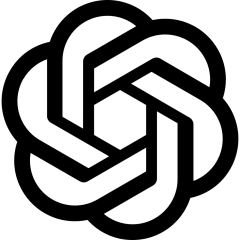
\includegraphics[width=7mm]{chapter/chapter_2/openai-icon-240x240.png}
            };
        \end{tcbcliptitle}
    },
    overlay first app ={
        \begin{tcbcliptitle}
            \node[anchor=north west] at (frame.north west) {
                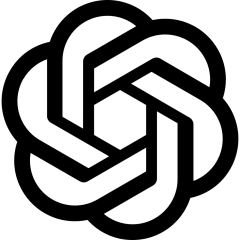
\includegraphics[width=7mm]{chapter/chapter_2/openai-icon-240x240.png}
            };
        \end{tcbcliptitle}
    }
]
\textbf{ChatGPT:} Nein, der Satz "Tomber dans les pommes" bedeutet nicht, dass die Bewohnerin dir Pommes zum Essen anbieten wollte. Tatsächlich ist es eine französische Redewendung, die einen Zustand beschreibt, in dem jemand ohnmächtig wird oder in Ohnmacht fällt. Die wörtliche Übersetzung ist "in die Äpfel fallen", aber im übertragenen Sinne bedeutet es, dass jemand kollabiert oder bewusstlos wird.

Diese Redewendung wird umgangssprachlich verwendet und ist im Französischen sehr geläufig, um einen plötzlichen Zustand der Bewusstlosigkeit oder des Zusammenbruchs zu beschreiben. Also, die Bewohnerin wollte dir keine Pommes anbieten, sondern sprach darüber, dass jemand ohnmächtig wird.
\tcbline
\textbf{Benutzer:} Sehr interessant, vielen Dank!
\tcbline
\textbf{ChatGPT:} Gern geschehen!
\end{tcolorbox}

Verglichen mit GPT-3.5 bietet GPT-4 grundlegend verbesserte Funktionen und Fähigkeiten \cite{openai-gpt-4-announcement}.
Eine weiterer Vergleich verbleibt somit zwischen OpenAIs Sprachmodellen GPT-3.5 und GPT-4, sowie Googles PaLM 2.

Ein grundlegendes Problem von Sprachmodellen ist, dass sie zu Halluzinationen neigen.
Es ist wichtig zu verstehen, dass wenn große Sprachmodelle auf enormen Datenmengen trainiert werden, sie die in diesen Daten enthaltenen statistische Muster und Strukturen erlernen \cite{basel-ml-arch}.
Als solches sind sie in der Lage Sätze oder Texte zu generieren, die kohärent wirken, ohne dabei wirklich ein wahres Verständnis des Textes oder ein Bewusstsein zu besitzen \cite{basel-ml-arch}.
Dies kann zu faktisch falschen oder unsinnigen Texterzeugnissen, auch Halluzinationen genannt, führen und sind Resultat von mangelndem Kontext und Textverständnis. \cite{sabre-pc-ai-hallucinations}.
Dieses Problem wird verstärkt durch veraltetes Wissen. 
So gilt für die meisten Sprachmodelle von OpenAI, auch GPT-4, dass ihre Trainingsdaten respektive ihr Wissen nach September 2021 abrupt enden \cite{openai-gpt-sep-2021}.
Dies ist für viele Anwendungsfälle dieser Sprachmodelle eine einschneidende Einschränkung, besonders für den Aspekt der Erklärbarkeit.
Ungeachtet dessen sind alle vorgestellten Sprachmodelle nachwievor von Natur aus Black-Boxes und weisen somit nur bedingt Erklärbarkeit auf.
Ein Argument für GPT-4 oder PaLM 2 ist, dass sie im Vergleich zu ihren Vorgängern jeweils eine wesentliche Verbesserung darstellen.
Eine besonders interessante Eigenschaft von PaLM 2 ist der Fokus auf Multilingualität, d.h. PaLM 2 wurde mit Daten in vielen Sprachen trainert \cite{google-palm2-techreport}.
Jedoch ist ihr Zugang entweder zur Zeit nicht vorhanden oder kann nur über eine Warteliste angefragt werden.
Seit dem 6. Juli 2023 erlaubt OpenAI den Zugriff auf das Sprachmodell GPT-4-8k für alle Anwender der Schnittstelle, die einen Verlauf erfolgreich abgeschlossener Zahlungen aufweisen \cite{openai-gpt4-access}.
Ein Argument für GPT-3.5 ist hingegen die Schnelligkeit im Vergleich zu GPT-4 und ein weitaus einfacher Zugriff über die Schnittstelle, die bereits über eine Anbindung für Java verfügt.
Im Rahmen dieser Arbeit wird für die folgende Modellierung und Implementierung GPT-3.5 / 4 als Vertreter zur Textgenerierung ausgewählt.

\paragraph{Schlussfolgerung}
Anhand der Erkenntnisse der beiden Diskussionen zur Wahl von Systemen zur Bild-, sowie Textgenerierung, fällt die Wahl eines Systems zur Bildgenerierung auf OpenAIs DALL·E 2, sowie die Wahl eines Systems zur Textgenerierung auf das Sprachmodelle GPT-3.5 und seiner Derivate, sowie eventuell auf andere von OpenAI angebotenen Sprachmodelle.
Diese Entscheidungen liegen in den folgenden Eigenschaften begründet:
\begin{itemize}
    \item Einfache Integration durch die offiziell von OpenAI unterstützte Community Bibliothek \enquote{OpenAI-Java} \cite{dall-e-java-api} für Java.
    \item Beide Systeme, DALL·E 2 und die GPT-Sprachmodelle, werden bereitgestellt durch eine einzige Plattform: OpenAI.
    \item Zahlung einfach und flexibel an einen einzigen Anbieter. 
    Zudem muss nur für das gezahlt werden, was wirklich genutzt wird, \textit{Only pay for what you use}, anstatt einer monatlichen Fixzahlung.
\end{itemize}
Die Wahl der primären Systeme liegt somit bei den oben genannten Systemen, deren Einsatz im weiteren Verlauf dieser Arbeit verfolgt wird.
Unabhängig von der Wahl der primären Systeme verbleiben die Systeme PaLM 2 oder Stable Diffusion weiterhin als optionale Kandidaten, die ebenfalls integriert werden könnten.

Die vorgestellten und ausgewählten Systeme bieten umfassende Möglichkeiten zur Bild- und Textgenerierung.
Jedoch existiert keine Benutzerschnittstelle im GMAF, die geeignete Interaktionsmöglichkeiten für Systeme generativer KI ermöglicht.
Dies führt zu einer weiteren, zweiten Herausforderung im Rahmen dieses Forschungsziels.

\begin{tcolorbox}[minipage, colback=white, colframe=black, arc=0pt, outer arc=0pt]
    \textbf{Offene Herausforderung OH 1.2 - Benutzerschnittstelle} \\
    Sollen diese Systeme im Rahmen des GMAF sinnvoll eingesetzt werden, um Erklärungen generieren zu können, so müssen Anwendern des GMAF durch eine Benutzerschnittstelle geeignete Interaktionsmöglichkeiten mit diesen Systemen geboten werden.
\end{tcolorbox}
Die offene Herausforderung \textbf{OH 1.2} wird im Rahmen einer Modellierung, sowie Implementierung ebenfalls in jeweils \hyperref[sec3:model:subsec:fz-explainability]{FZ 1.2/TB} und \hyperref[sec4:impl:subsec:fz-explainability]{FZ 1.3/I} angesprochen und untersucht. 

Im nächsten Abschnitt werden die im Rahmen dieses Forschungsziels identifizierten offenen Herausforderungen zusammengefasst.

\paragraph{Offene Herausforderungen}
\label{sec2:sota:par:fz1:open-challenges}
In \cref{sec2:sota:subsubsec:gmaf,sec2:sota:subsubsec:mmfg,sec2:sota:subsubsec:graph-codes} wurden Technologien in Bezug auf das GMAF vorgestellt.
Es konnte festgestellt werden, dass der Ansatz MMFGs bzw. Graph Codes erklärbar zu machen, sehr statistisch und rein mathematischer Natur ist.
Eine Verbesserung bzw. einen alternativen Ansatz, um MMFGs bzw. Graph Codes erklärbar machen zu können, verspricht der Einsatz von Systemen generativer KI.
Dies führt zur ersten offenen Herausforderung \textbf{OH 1.1} und der Frage \enquote{Wie kann generative KI eingesetzt werden, um Erklärbarkeit zu erreichen?}.
% Eventuell Unterschied zwischen Erklärbarkeit von generativer KI und Erklärbarkeit durch generative KI hervorheben?
Es gilt daher im Rahmen der Umgebung \enquote{Erklärbarkeit von MMIR mittels generativer KI} zu ermitteln, wie Systeme generativer KI genutzt werden können, um Erklärbarkeit zu erreichen bzw. Erklärungen zu generieren.

Im weiteren Verlauf wurden im \cref{sec2:sota:subsubsec:genai} grundlegende Technologien, Techniken und Eigenschaften beschrieben und eine Reihe an Systemen generativer KI vorgestellt.
Aus dieser Reihe an Systemen wurde in \cref{sec2:sota:subsubsec:fz1:discussion} eine Auswahl an Systemen getroffen, deren Einsatz im weiteren Verlauf dieser Arbeit verfolgt werden.
Die in diesem Abschnitt vorgestellten und ausgewählten Systeme bieten umfassende Möglichkeiten zur Bild- und Textgenerierung.
Sollen diese Systeme im Rahmen des GMAF sinnvoll eingesetzt werden, um Graph Codes erklärbar zu machen, so müssen Anwendern des GMAF durch eine Benutzerschnittstelle geeignete Interaktionsmöglichkeiten mit diesen Systemen geboten werden.
Es konnte festgestellt werden, dass das GMAF für seine Anwender keine Interaktionsmöglichkeiten mit Systemen generativer KI bietet.
Dies führt zur zweiten offenen Herausforderung \textbf{OH 1.2} und der Frage \enquote{Wie muss eine Benutzerschnittstelle beschaffen sein, um geeignete Interaktionsmöglichkeiten mit Systemen generativer KI zu ermöglichen?}.
%Es gilt daher die Funktionen dieser Systeme für die Umgebung \enquote{Erklärbarkeit von MMIR mittels generativer KI} im Rahmen des GMAF und in einem eigens dafür bestimmten Programm oder als Erweiterung in das GMAF anhand von Anwendungsfällen zu integrieren.
Es gilt daher anhand von Anwendungsfällen geeignete Schnittstellen zur Interaktion mit den in diesem Abschnitt vorgestellten Systemen generativer KI für die Umgebung \enquote{Erklärbarkeit von MMIR mittels generativer KI} im Rahmen des GMAF in einem eigens dafür bestimmten Programm oder als Erweiterung in das GMAF umzusetzen.

Die beiden offenen Herausforderungen \textbf{OH 1.1} und \textbf{OH 1.2} werden im Rahmen einer Modellierung durch das Forschungsziel FZ 1.2/TB angesprochen und durch das Forschungsziel 1.3/I im Rahmen einer prototypischen Implementierung untersucht.
Forschungsziel 1.4/E wird sich der Evaluierung der in diesen Kapiteln erlangten Forschungsergebnissen widmen.

\clearpage

\subsection{FZ 2.1/O Integration generativer KI in das GMAF}
\label{sec2:sota:subsec:fz-integration}
Dieser Abschnitt gibt einen Überblick über ausgewählte Ergebnisse und Erkenntnisse aus der Forschung im Bereich der Integration von Systemen generativer KI und deckt technische Aspekte ab, die sich auf die zweite Problembeschreibung beziehen.
\cref{sec2:sota:subsubsec:gc-capabilities-integration} widmet sich den Integrationsmöglichkeiten von Graph Codes.
Weiter befasst sich \cref{sec2:sota:subsubsec:genai-capabilities-integration} mit den Integrationsmöglichkeiten von Systemen generativer KI.

\subsubsection{Integrationsmöglichkeiten von Graph Codes}
\label{sec2:sota:subsubsec:gc-capabilities-integration}
Dieser Abschnitt befasst sich mit den Integrationsmöglichkeiten von Graph Codes.
Wie bereits in \cref{sec2:sota:subsubsec:graph-codes} beschrieben, sind Graph Codes eine Technologie zur effizienten und effektiven Darstellung und Verarbeitung von Merkmalen im GMAF.
Als solches ist eine Integration von Graph Codes im Rahmen des GMAF bereits gegeben.
Diese Integration bietet im Rahmen des GMAF folgende Komponenten:
\begin{itemize}
    \item \textit{GraphCode} bietet eine Implementierung der zweidimensionalen Darstellung von Merkmalen und ermöglicht Zugriff auf das Wörterbuch eines Graph Codes.
    \item \textit{GraphCodeCollection} bietet eine Reihe an Operationen, wie z.B. die Vereinigung oder Subtraktion von Graph Codes an.
    \item \textit{GraphCodeGenerator} ist eine Implementierung, die das Erstellen eines Graph Codes aus einem MMFG ermöglicht.
    \item \textit{GraphCodeIO} bietet eine Reihe an nützlichen Operationen zum Import oder Export von Graph Codes aus oder in Dateien.
    \item \textit{GraphCodeMetric} bietet eine Implementierung der in \cref{sec2:sota:par:gc-similiarity} beschriebenen Metrik zur Ähnlichkeit von Graph Codes.
\end{itemize}

Die grundsätzliche Darstellungsform eines Graph Codes erfolgt im textbasierten Dateiübertragungsformat JSON (JavaScript Object Notation) und kann somit leicht von Menschen, aber auch Maschinen gelesen und verarbeitet werden.
\cref{sec2:sota:subsec:fz2:lst:gc-ex-json} zeigt das Beispiel des Graph Codes $GC_{ex}$ in JSON-Format.
\begin{lstlisting}[
    language=json,
    firstnumber=1,
    label={sec2:sota:subsec:fz2:lst:gc-ex-json},
    captionpos=b,
    caption={Beispiel des Graph Codes $GC_{ex}$ im JSON-Format.}
]
{
  "dictionary": [
    "root-image",
    "person",
    "body",
    "arm",
    "watch"
  ],
  "collectionElements": [],
  "matrix": [
    [1,1,0,0, 0],
    [0,1,1,0, 0],
    [0,0,1,1, 0],
    [0,0,0,1,17],
    [0,0,0,0, 2]
  ]
}
\end{lstlisting}

Dieses Beispiel zeigt, wie die Informationen eines Graph Codes, wie z.B. das Wörterbuch oder die Wertungsmatrix, als ein Objektgraph bestehend aus mehreren Paaren von Schlüssel und Werten im Syntax \textbf{Schlüssel : Wert} dargestellt werden.
Im Falle der Paare aus Schlüsseln und Werten stellen Schlüssel immer eine Zeichenfolge, wie \enquote{dictionary}, \enquote{collectionElements} oder \enquote{matrix} dar, während Werte Zahlen, Strings, Arrays oder wiederum Objekte sein können.
Die Elemente \enquote{dictionary} und \enquote{collectionElements} haben jeweils Arrays als Werte, in welchen eine Menge an Bezeichnern bzw. Graph Codes enthalten sein können.
Da die gesamte Darstellung eines Graph Codes im JSON-Format wiederum ein Objekt ist, kann \enquote{collectionElements} eine Menge bzw. Sammlung an Darstellungen von Graph Codes enthalten.
Auf diese Weise kann eine rekursive Darstellung von Graph Codes erreicht werden.
Das Element \enquote{matrix} hat ebenfalls ein Array als Wert. 
Da allerdings die Adjanzenzmatrix eine zweidimensional Matrix ist, sind die Werte im Array wiederum Arrays aus ganzen Zahlen mit einer Länge, die äquivalent zu Größe des Wörterbuchs ist.
Das GMAF integriert bereits für die Verarbeitung und Operationen mit JSON die GSON \cite{gson} Bibliothek von Google ein.

Auch wenn Systeme wie GPT-3.5 oder GPT-4 und PaLM 2 in der Lage sind Daten im JSON-Format in Textform zu verarbeiten, so bleibt jedoch offen, wie die Informationen aus einem Graph Code und die damit assoziierten Informationen in die Eingabe für ein System generativer KI überführt werden kann, und welche Eigenheiten berücksichtigt werden müssen.
Dies führt zu einer ersten offenen Herausforderung im Rahmen dieses Forschungsziels.
\begin{tcolorbox}[minipage, colback=white, colframe=black, arc=0pt, outer arc=0pt]
    \textbf{Offene Herausforderung OH 2.1 - Transformieren von Graph Codes} \\
    Umwandlung von Graph Codes in eine passende Eingabeform für Systeme generativer KI.
\end{tcolorbox}
Die offene Herausforderung \textbf{OH 2.1} wird im Rahmen einer Modellierung, sowie Implementierung in jeweils \hyperref[sec3:model:subsec:fz-integration]{FZ 2.2/TB} und \hyperref[sec4:impl:subsec:fz-integration]{FZ 2.3/I} angesprochen und untersucht. 

\subsubsection{Integrationsmöglichkeiten von Systemen generativer KI}
\label{sec2:sota:subsubsec:genai-capabilities-integration}
Dieser Abschnitt befasst sich mit den Möglichkeiten der Integration der in \cref{sec2:sota:subsubsec:fz1:discussion} ausgewählten Systeme generativer KI.
Dies sind in erster Linie die Systeme, GPT-3.5/4 und Dall-E, die von OpenAI entwickelt wurden.
OpenAI bietet zur Übersicht eine Plattform für seine Produkte an.
Diese Plattform umfasst neben den Produkten auch Anleitungen, Beispiele und Tipps zu bewährten Praktiken zu diesen Produkten und beschreibt eine Reihe an Möglichkeiten zur Integration seiner Produkte.
Diese Integrationsmöglichkeiten umfassen:
\begin{itemize}
    \item Eine Schnittstelle (API), die es Entwicklern ermöglicht Modelle in ihre eigene entwickelte Software zu integrieren und aufzurufen.
    \item Unterstützte Systeme zur Softwareentwicklung (SDKs) in vielen Programmiersprachen, die u.a von OpenAI bereitgestellt werden, oder von Mitgliedern der Community in anderen, nicht offiziell von OpenAI unterstützten Programmiersprachen entwickelt wurden \cite{openai-community-library}.
    \item Online-Dienste, die es Entwicklern ermöglichen Modelle ohne eigens entwickelte Software zu verwenden.
    Beispiele für diese Online-Dienste sind ChatGPT, Dall-E, Tokenizer oder ein Textklassifikator für KI.
    % https://platform.openai.com/tokenizer
    % https://platform.openai.com/ai-text-classifier
    \item Cloud-Dienste, die es Entwicklern ermöglichen Modelle ohne eigene Infrastruktur zu verwenden \cite{openai-cloud-services}.
\end{itemize}
Im nächsten Abschnitt wird gesondert auf die Schnittstelle und die Systeme zur Softwareentwicklung eingegangen.
Im darauffolgenden \cref{sec2:sota:par:tokenizer} werden dann weitere interessante Werkzeuge im Rahmen der Schnittstelle von OpenAI besprochen und Aspekte hervorgehoben.

\paragraph{API}
\label{sec2:sota:par:api}
Eine Schnittstelle (engl. \textbf{A}pplication \textbf{P}rogramming \textbf{I}nterface) ermöglicht Entwicklern die Kommunikation zwischen Softwareanwendungen umzusetzen.
Eine API definiert und stellt Funktionen bereit, die Entwickler verwenden können, um Softwareanwendungen miteinander zu verbinden.
Funktionen können das Auslesen und Schreiben von Daten, oder Ausführen von Aktionen in einer anderen Anwendung sein.
Auf diese Weise ermöglicht eine Schnittstelle den Zugriff auf Funktionen einer Anwendung, ohne dass diese in einer Anwendung selbst neu geschrieben bzw. programmiert werden müssen.

Die API von OpenAI kann praktisch auf jede Aufgabe angewendet werden, die das Verstehen oder Erzeugen von natürlicher Sprache betrifft und erfordert \cite{openai-docs-intro}.
Des Weiteren kann die API auch verwendet werden, um Bilder zu erzeugen, zu bearbeiten oder Sprache in Text zu konvertieren \cite{openai-docs-intro}.
Die API von OpenAI bietet Zugriff auf eine Reihe von Modellen, die unterschiedliche Fähigkeiten und Preise aufweisen \cite{openai-docs-intro}.

Die Schnittstelle von OpenAI wird durch eine RESTful (Representational State Transfer) Schnittstelle bereitgestellt.
REST-Schnittstellen sind eine der prominenteste Arten von APIs \cite{postman-state-of-api-2023}, die eine Reihe an Konventionen verwenden, um die Verarbeitung und Übertragung von Informationen zu gewährleisten.
Diese RESTful Schnittstelle wird spezifiziert über eine OpenAPI Spezifikationen \cite{openai-openapi-spec}, die die Funktionen der OpenAI Schnittstelle genaustens dokumentiert.
OpenAPI ist eine auf dem Architekturstil REST basierende Spezifikationssprache für die Beschreibung der Struktur, der Reihenfolge und des Verhaltens von APIs.
Diese Spezifikation wird für gewöhnlich in YAML oder JSON geschrieben und kann, neben der Dokumentation einer API, auch dazu verwendet werden, um mit spezialisierten Programmen, wie z.B. Swagger Codegen, automatisch Quellcode in einer spezifischen Programmiersprache zu generieren.
% https://swagger.io/tools/swagger-codegen/
Für die Programmiersprache Java wird diese Spezifikation bereits durch die SDK bzw. Bibliothek OpenAI-Java \cite{dall-e-java-api} abgedeckt.

Die API von OpenAI bietet Zugriff auf folgende Endpunkte:
\begin{enumerate}
    \item /v1/completions
    \item /v1/chat/completions
    \item /v1/edits
    \item /v1/images/generations
    \item /v1/images/edits
    \item /v1/images/variations
    \item /v1/embeddings
    \item /v1/audio/transcriptions
    \item /v1/audio/translations
    \item /v1/files
    \item /v1/fine-tunes
    \item /v1/moderations
\end{enumerate}
Im Rahmen dieser Arbeit sind nur die Endpunkte 2 und 4 zur Generierung von Text bzw. Bildern von Interesse.
In \cite{openai-api-doc} wird eine genaue Dokumentation, mitsamt Beispielen für diese Endpunkte beschrieben.

Eine Anfrage an den Endpunkt \textbf{/chat/completions/} nimmt als Eingabe eine Liste an Nachrichten in Form einer Unterhaltung zwischen verschiedenen Parteien.
Eine Nachricht besteht dabei aus einem Wertepaar \textbf{Rolle} : \textbf{Inhalt}.
Beide Werte sind notwendige Parameter einer Anfrage an diesen Endpunkt.
Der Parameter \textit{Rolle} kann einen von drei Werten annehmen: \textit{System}, \textit{Assistant}, \textit{User} \cite{openai-chat-compl-roles}.
Über den Endpunkt liefert das Modell eine Antwort auf diese Unterhaltung.

Eine Anfrage an den Endpunkt \textbf{/images/generations/} nimmt als Eingabe eine Eingabeaufforderung bzw. Prompt.
Das Modell generiert anhand dieser Prompt ein oder mehrere Bilder und liefert diese über den Endpunkt als Antwort zurück.

Die in diesem Abschnitt vorgestellte Schnittstelle mit all ihren Endpunkten bietet bereits umfassende Möglichkeiten zur Generierung von Text und Bildern.
Allerdings gibt es keine bestehende Integration dieser Systeme generativer KI im GMAF.
Dies führt zu zweiten, offenen Herausforderung im Rahmen dieses Forschungsziels.
\begin{tcolorbox}[minipage, colback=white, colframe=black, arc=0pt, outer arc=0pt]
    \textbf{Offene Herausforderung OH 2.2 - Integration generativer KI} \\
    Zum Zeitpunkt des Verfassens dieser Arbeit existiert keine Integration der von OpenAI angebotenen Systeme generativer KI im GMAF.
\end{tcolorbox}
Die offene Herausforderung \textbf{OH 2.1} wird im Rahmen einer Modellierung, sowie Implementierung ebenfalls in jeweils \hyperref[sec3:model:subsec:fz-integration]{FZ 2.2/TB} und \hyperref[sec4:impl:subsec:fz-integration]{FZ 2.3/I} angesprochen und untersucht. 

\paragraph{Tokenizer}
\label{sec2:sota:par:tokenizer}
Neben der Schnittstelle bietet OpenAI eine Reihe an Werkzeugen bzw. Online-Diensten an.
Eines dieser Werkzeuge ist der Tokenizer.
Die GPT-Modellreihe benutzt zum Verarbeiten von Text sogenannte Tokens \cite{openai-tokenizer}.
Tokens stellen häufige im Text vorkommende Zeichenfolgen dar \cite{openai-tokenizer}.
Die GPT-Modelle verstehen die statistischen Beziehungen zwischen diesen Token und sind anhand dieser Beziehungen und der bereits bestehenden Folge an Token im Text in der Lage das nächste Token im Text zu erzeugen \cite{openai-tokenizer}.
Ein abgewandeltes Beispiel für eine Tokenaufteilung ist im folgenden Text einsehbar:

\enquote{\sethlcolor{tok1}\hl{Multiple}\sethlcolor{tok2}\hl{ models}\sethlcolor{tok3}\hl{,}\sethlcolor{tok4}\hl{ each}\sethlcolor{tok5}\hl{ with}\sethlcolor{tok1}\hl{ different}\sethlcolor{tok2}\hl{ capabilities}\sethlcolor{tok3}\hl{ and}\sethlcolor{tok4}\hl{ price}\sethlcolor{tok5}\hl{ points}\sethlcolor{tok1}\hl{.}\sethlcolor{tok2}\hl{ Prices}\sethlcolor{tok3}\hl{ are}\sethlcolor{tok4}\hl{ per}\sethlcolor{tok5}\hl{ }\sethlcolor{tok1}\hl{1}\sethlcolor{tok2}\hl{,}\sethlcolor{tok3}\hl{000}\sethlcolor{tok4}\hl{ tokens}\sethlcolor{tok5}\hl{.}\sethlcolor{tok1}\hl{ You}\sethlcolor{tok2}\hl{ can}\sethlcolor{tok3}\hl{ think}\sethlcolor{tok4}\hl{ of}\sethlcolor{tok5}\hl{ tokens}\sethlcolor{tok1}\hl{ as}\sethlcolor{tok2}\hl{ pieces}\sethlcolor{tok3}\hl{ of}\sethlcolor{tok4}\hl{ words}\sethlcolor{tok5}\hl{,}\sethlcolor{tok1}\hl{ where}\sethlcolor{tok2}\hl{ }\sethlcolor{tok3}\hl{1}\sethlcolor{tok4}\hl{,}\sethlcolor{tok5}\hl{000}\sethlcolor{tok1}\hl{ tokens}\sethlcolor{tok2}\hl{ is}\sethlcolor{tok3}\hl{ about}\sethlcolor{tok4}\hl{ }\sethlcolor{tok5}\hl{750}\sethlcolor{tok1}\hl{ words}\sethlcolor{tok2}\hl{.}\sethlcolor{tok3}\hl{ This}\sethlcolor{tok4}\hl{ paragraph}\sethlcolor{tok5}\hl{ is}\sethlcolor{tok1}\hl{ }\sethlcolor{tok2}\hl{49}\sethlcolor{tok3}\hl{ tokens}\sethlcolor{tok4}\hl{.}} Encoding: \textit{(cl100k\_base)} \cite{openai-model-tiktoken}

Die Aufteilung der Zeichenfolgen in Tokens ist abhängig vom jeweiligen Modell und kann in \cite{openai-model-tiktoken} eingesehen werden.
Die Aufteilung eines Textes in Tokens ist deshalb interessant, da durch dieses Werkzeug die Anzahl der Tokens bestimmt werden kann.
In Kombination dieser Information und der Information zur Bepreisung kann ein potentielles Optimierungspotenzial in Bezug auf die Anzahl der Tokens und somit auch der Bepreisung ausgeschöpft werden.

Der Online-Dienst Tokenizer von OpenAI ist offiziell durch die für Python konzipierte Bibliothek \enquote{Tiktoken} \cite{openai-python-tiktoken} oder inoffiziell durch die für Java konzipierte Bibliothek \enquote{JTokkit} \cite{openai-java-jtokkit} als Schnittstelle für die Tokenisierung von Text verfügbar.

\subsubsection{Diskussion}
\label{sec2:sota:subsubsec:fz2:discussion}
In diesem Abschnitt wurden die Möglichkeiten der Integration von Graph Codes, sowie den von OpenAI angebotenen Systemen generativer KI behandelt.

In Bezug auf die Integrationsmöglichkeiten von Graph Codes konnte eine Übersicht über die vom GMAF gebotenen Komponenten, die eine entscheidende Rolle in der Technik der Graph Codes spielen, zusammengestellt werden.
Es wurde weiterhin bestimmt, dass die Darstellungsform der in Graph Codes enthaltenen Informationen im JSON-Format erfolgt.
Diese Darstellungsform kann insbesondere von aktuellen Systemen generativer KI effizient und effektiv eingelesen werden.

In Bezug auf die Integrationsmöglichkeiten der von OpenAI entwickelten Systemen generativer KI konnte eine Übersicht über die von OpenAI bereitgestellte Schnittstelle gegeben werden.
Diese Übersicht gibt auch Einblick über die verfügbaren Endpunkte und Einbindungsmöglichkeiten dieser Endpunkte über eine speziell für Java entwickelte Bibliothek bzw. SDK für eine einfache Integration in das GMAF.
Des Weiteren wurde das Tool Tokenizer, welches im Umgang mit den Modellen eine wichtige Rolle spielen kann, genauer erklärt und in eine potentielle Nutzung eingeordnet. 

\paragraph{Offene Herausforderungen}
\label{sec2:sota:par:fz2:open-challenges}
In \cref{sec2:sota:subsubsec:gc-capabilities-integration} wurde die Erkenntnis erlangt, dass Graph Codes zur Darstellung im bekannten Dateiübertragungsformat JSON dargestellt werden.
Auch wenn die von OpenAI angebotenen Modelle in der Lage sind JSON zu verstehen und analysieren, so bleibt offen, wie eine Umwandlung von Graph Codes in eine geeignete Eingabeform für Systeme generativer KI erfolgen kann.
Dies führt zur ersten, offenen Herausforderung \textbf{OH 2.1} im Rahmen dieses Forschungsziels.
Es gilt daher eine geeignete Überführung der Graph Codes in Systeme generativer KI für die Umgebung \enquote{Integration generativer KI in das GMAF} zu bestimmen.

Im weiteren Verlauf wurde in \cref{sec2:sota:subsubsec:genai-capabilities-integration} eine Übersicht über die von OpenAI bereitgestellte Schnittstelle, mitsamt ihrer verfügbaren Endpunkte, und ihrer Einbindungsmöglichkeiten geschaffen.
Es konnte festgestellt werden, dass das GMAF bisher keine Einbindung dieser Endpunkte über die Schnittstelle und folglich auch keinen Systeme generativer KI umsetzt.
Dies führt zur zweiten, offenen Herausforderung \textbf{OH 2.2} im Rahmen dieses Forschungsziels.
Es gilt daher die Funktionen der Schnittstelle zu den Endpunkten der in \cref{sec2:sota:subsubsec:fz1:discussion} ausgewählten Systeme generativer KI für die Umgebung \enquote{Integration generativer KI in das GMAF} zu integrieren.

Die beiden offenen Herausforderungen \textbf{OH 2.1} und \textbf{OH 2.2} werden im Rahmen einer Modellierung durch das Forschungsziel FZ 2.2/TB angesprochen und durch das Forschungsziel 2.3/I im Rahmen einer prototypischen Implementierung untersucht.
Forschungsziel 2.4/E wird sich der Evaluierung der in diesen Kapiteln erlangten Forschungsergebnissen widmen.

\clearpage

\subsection{Evaluierungsmethodiken}
\label{sec2:sota:subsec:eval-methodology}
Die Evaluierung ist ein entscheidender Teil im Zyklus der Softwareentwicklung und dient der Beurteilung der Qualität, Korrektheit und Einhaltung von Standards und Vorschriften.
In diesem Abschnitt werden eine Reihe bekannter Evaluierungsmethodiken zur systematischen Evaluierung in der Softwareentwicklung vorgestellt.
Mit Hilfe dieser Evaluierungsmethodiken lassen sich besagte Bewertungen der im Rahmen dieser Arbeit implementierten prototypischen Software vornehmen.

Das IEEE \cite{ieee} bietet mit der Norm IEEE 1028-2008 \cite{ieee-1028-2008} Richtlinien zur Durchführung von Softwareüberprüfungen.
Diese Softwareüberprüfungen sind, formal betrachtet, Evaluierungen von in der Entwicklungen entstandenen Software-Artifakten, um Defekte festzustellen, die Qualität zu verbessern und sicherzustellen, dass alle Vorschriften eingehalten werden.
Die Norm 1028-2008 definiert mehrere Arten von Peer-Review-Verfahren, die im Zyklus der Softwareentwicklung Verwendung finden können.
Ein Peer-Review-Verfahren ist ein Prozess, in welchem die Ergebnisse der Softwareentwicklung manuell von einem oder mehreren im selben Feld tätigen Experten bzw. Kollegen überprüft werden.
Folgende Peer-Review-Verfahren sind in der Norm IEEE 1028-2008 definiert:
\begin{itemize}
    \item Informal Review
    \item Technical Review
    \item Walkthrough
    \item Inspection
    \item Audit
\end{itemize}
Im Folgenden werden diese einzelnen Verfahren kurz erläutert und ihre Verwendung, der Ablauf, sowie die Vor- und Nachteile näher beschrieben.

\textbf{Informal Review} (z.Dt. informeller Review) ist ein einfaches und flexibles Verfahren, um in erster Instanz nach Defekten zu suchen und Rückmeldungen zu Software-Artifakten zu erhalten, ohne dabei aktiv Programmcode auszuführen. 
Es werden im Rahmen von informellen Reviews keine Dokumentationen angefertigt.
%In informellen Reviews wird keine Dokumentation angefertigt.
Der Ablauf eines informellen Reviews sieht es vor, dass Prüfer die Dokumentation der Software oder ihren Quellcode individuell untersuchen und anhand ihrer Erfahrungen und Expertise Rückmeldungen liefern.
Der Vorteil an informellen Reviews ist, dass sie einfach, schnell und kostengünstig umsetzbar sind.
Des Weiteren kann dieses Verfahren bereits in den allerersten Schritten der Entwicklung durchgeführt werden, um frühzeitig Defekten vorzubeugen und Einblicke zu erlangen.
Nachteilig an einem informellen Review ist der Mangel an einem strukturierten Vorgehen und mangelnder Gründlichkeit der Untersuchungen.
%Nachteilig an einem informellen Review ist der Mangel an einem strukturierten Vorgehen, was zu Problemen in Bezug auf die Widerspruchsfreiheit und Vollständigkeit des Verfahrens führt.
%Zudem kann die mangelnde Gründlichkeit der Untersuchungen dazu führen, dass Defekte potentiell nicht erfasst werden.

\textbf{Technical Review} (z.Dt. technischer Review) ist, verglichen mit einem informellen Review, ein detailliertes Verfahren zur Evaluierung von Software-Artifakten, um die Eignung des zu testenden Artifakts für die beabsichtigte Nutzung festzustellen.
Schwerpunkte eines technischen Reviews liegen dabei im Einhalten von Standards und Normen, Korrektheit und Vollständigkeit der überprüften Artifakte.
Der Ablauf eines technischen Reviews sieht es vor, dass Prüfer die Artifakte gründlich gegen die in den Vorgaben festgelegten Kriterien, wie Spezifikationen und Standards, prüfen und Abweichungen genaustens dokumentieren.
Der Vorteil an technischen Reviews ist, dass sie durch eine eingehende Analyse und Bewertung der Software-Artifakte die Einhaltung von Spezifikationen, Normen und Standards garantieren und aufgrund ihrer gründlichen Natur technische Defekte identifizieren können.
%Nachteilig an einem technischen Review ist, dass es aufgrund der detaillierten Überprüfung sehr ressourcenintensiv ist und Planung, Zeit und Expertise benötigt.

\textbf{Walkthrough} (z.Dt. Durchlauf) ist ein Verfahren, in welchem die Vorgehensweise von einem Autor in einer Durchführung durch die Software beschrieben wird.
Ziel dieser Durchführung ist es, die Beteiligten mit den Software-Artifakten vertraut zu machen, um Rückmeldungen und Klarstellungen von ihnen zu erhalten.
Der oder die Autor(en) der Artifakte demonstrieren diese den Teilnehmern des Durchlaufs, um Rückmeldungen über die vorgestellten Artifakte zu erhalten.
Teilnehmer dieses Durchlaufs sind für gewöhnlich eine andere Partei, wie z.B. Arbeitskollegen.
Rückmeldungen über die vorgestellten Artifakte enthalten zumeist Fragen, Kommentare oder Verbesserungsvorschläge zu den wahrgenommenen Abweichungen oder Mängeln in der Software im Vergleich zum beschriebenen Ablauf.
Der Vorteil an einem Durchlauf ist, dass er die Zusammenarbeit und den Austausch von Wissen zwischen den Beteiligten fördert.
Mit Hilfe eines Durchlaufs können Fehler identifiziert, das Verständnis verbessert und unterschiedliche Perspektiven gesammelt werden.
Es wird somit die Gültigkeit des beschriebenen Ablaufs bzw. Lösungsvorschlags für die Software geprüft.
Eine weit verbreitete Variante des Walkthroughs ist der \textbf{Cognitive Walkthrough}.
Im Vergleich zu einem simplen Durchlauf ist ein Cognitive Walkthrough speziell auf die Bewertung der Benutzerfreundlichkeit und Benutzererfahrung ausgelegt.
Ein simpler Durchlauf kann eher als allgemeines Verfahren zur Prüfung von Software verstanden werden, welches verschiedene Aspekte der Softwareentwicklung umfasst.
An einem Cognitive Walkthroguh sind für gewöhnlich sogenannte \textbf{Usability-Experten} beteiligt. 
Aufgabe der Usability-Experten ist es, die Perspektive eines potentiellen Nutzers einzunehmen, während in einem simplen Durchlauf in der Regel nur Teammitglieder oder andere Interessensgruppen beteiligt sind, die anhand ihres Fachwissens Rückmeldungen und Erkenntnisse liefern.
%Nachteilig an einem Cognitive Walkthrough ist, dass aufgrund mangelnder Struktur und Gründlichkeit potentielle Defekte unentdeckt bleiben können.

\textbf{Inspection} ist ein streng formales Verfahren, welches die Eignung bzw. Beschaffenheit eines Arbeitsergebnisses für die beabsichtigte Verwendung untersucht.
Das Verfahren hat zum Ziel Defekte in Software-Artifakten zu identifizieren und die Qualität der Software-Artifakte zu garantieren, sowie zu verbessern \cite{ieee-1028-2008}.
Der Ablauf einer Inspection sieht vor, dass ein Team, welches von einem Moderator geleitet wird, die Software-Artifakte gründlich und systematich gegen ihre vorgegebenen Standards und Ansprüche prüft \cite{ieee-1028-2008}.
Defekte und Widersprüche werden festgestellt und klar dokumentiert \cite{ieee-1028-2008}.
Der Vorteil an einer Inspection ist, dass sie einen klaren strukturierten und disziplinierten Ansatz zur Fehlererkennung verfolgen.
Weiterhin werden im Rahmen einer Inspection die Untersuchungen von ausgebildeten Inspektoren vorgenommen \cite{ieee-1028-2008}.
Diese Eigenschaften machen eine Inspection zu einem wirksamen Ansatz zur Fehlerentdeckung und Verbesserung der Gesamtqualität von Software-Artifakten.
%Ein Nachteil einer Inspection ist der Zeitaufwand, dem, vor allem bei größeren Projekten, das strenge formale Verfahren, sowie die Abstimmung zwischen den involvierten Personen zugrunde liegen.

\textbf{Audit} ist ein Verfahren, das umfassende Bewertungen von Software-Artifakten zum Ziel hat, um Übereinstimmungen bzw. Diskrepanzen mit Anforderungen, Vorschriften oder Standards zu beurteilen.
Der Ablauf eines Audits sieht vor, dass Auditoren Software-Artifakte und Dokumentationen prüfen und diese mit den vorgegebenen Anforderungen vergleichen.
Abweichungen werden festgestellt und klar dokumentiert.
Der Vorteil an einem Audit ist, dass durch umfassende Bewertungen von Software-Artifakten die Einhaltung von Vorschriften garantiert wird und zudem verbesserungsdürftige Bereiche aufzeigt werden.

Nachteile der genannten Peer-Review-Verfahren sind vor allem zumeist die Zuweisung von Ressourcen, wie z.B. von Zeit, der Definition des genauen Vorgehens, potentielle Voreingenommenheiten bzw. Dynamiken zwischen Prüfern und Teilnehmern, sofern sie aus einer Organsation kommen und nicht unabhängig voneinander arbeiten und begrenzter Fachkenntnisse und Expertise von Prüfern.

Die in diesem Abschnitt vorgestellten Verfahren bzw. Methodiken bieten einen Überblick über eine Bandbreite an Möglichkeiten zur Evaluierung von Software. 
Eine Auswahl aus diesen Evaluierungsmethodiken wird am Anfang in Kapitel 5 vorgenommen.

\clearpage

\subsection{Zusammenfassung}
\label{sec2:sota:subsec:summary}
In diesem Kapitel wurde die Recherche zum bisherigen Stand der Wissenschaft und Technik zur Erklärbarkeit und Visualisierung von Graph Codes mittels generativer KI behandelt.
In \cref{sec2:sota:subsubsec:summary-remaining-open-challenges} werden die noch offenen und verbleibenden Herausforderungen zusammengefasst.
Weiter werden in \cref{sec2:sota:subsubsec:summary-findings} die wesentlichen Ergebnisse und Erkenntnisse dieser Recherche nach den Forschungszielen der Beobachtungsphase, wie nach der Methodik von Nunamaker vorgesehen, aufgeschlüsselt und kurz zusammengefasst.
In \cref{sec2:sota:subsubsec:summary-decisions} werden die Entscheidungen der Diskussionen der behandelten Forschungsziele aufgezählt.
Schlussendlich wird in \cref{sec2:sota:subsubsec:summary-handling-open-challenges} die Behandlung der noch offenen Herausforderungen angesprochen.
Schlussendlich gibt \cref{sec2:sota:subsec:summary:table:summary} eien Gesamtübersicht über den aktuellen Stand der Arbeit.

\subsubsection{Welche offenen Herausforderungen (OH) verbleiben?}
\label{sec2:sota:subsubsec:summary-remaining-open-challenges}
In diesem Abschnitt werden die noch offenen und verbleibenden Herausforderungen, die sich im Rahmen der Recherche zum Stand der Wissenschaft und Technik ergeben haben, aufgezählt, kurz beschrieben und jeweils Verortungen der Lösungsansätze genannt.

\begin{xltabular}{\linewidth}{
            @{}
            >{
                \hsize=0.2\linewidth
                \centering\arraybackslash
            }X
            >{
                \hsize=0.6\linewidth
            }X
            >{
                \hsize=0.2\linewidth
                \raggedright\arraybackslash
            }X
            @{}
        }

        \caption{Offene Herausforderungen}
        \label{sec2:sota:subsec:summary:table:open-issues}
        \\

        \toprule
        % First Row
        \multicolumn{1}{
            >{
                \hsize=0.2\linewidth\centering\arraybackslash
            }X
        }{
            \textbf{Nummer der offenen Herausforderungen}
        } & \multicolumn{1}{
            >{
                \hsize=0.6\linewidth\centering\arraybackslash
            }X
        }{
            \textbf{Inhalt der offenen Herausforderungen}
        } & \multicolumn{1}{
            >{
                \hsize=0.2\linewidth\centering\arraybackslash
            }X
        }{
            \textbf{Ansatz für Lösung}
        } \\

        \midrule

        \endfirsthead

        \toprule
        % First Row
        \multicolumn{1}{
            >{
                \hsize=0.2\linewidth\centering\arraybackslash
            }X
        }{
            \textbf{Nummer der offenen Herausforderungen}
        } & \multicolumn{1}{
            >{
                \hsize=0.6\linewidth\centering\arraybackslash
            }X
        }{
            \textbf{Inhalt der offenen Herausforderungen}
        } & \multicolumn{1}{
            >{
                \hsize=0.2\linewidth\centering\arraybackslash
            }X
        }{
            \textbf{Ansatz für Lösung}
        } \\

        \midrule

        \endhead

        % Lower Rows

        \hyperref{sec2:sota:oi:1.1}{OH 1.1}
        &
        Es existiert keine Möglichkeit oder Untersuchung Systeme generativer KI zur Erklärbarkeit von Graph Codes zu nutzen.
        Es bleibt daher offen, ob und wie durch den Einsatz von generativer KI Erklärbarkeit erreicht werden kann.
        % Offen bleibt, wie durch den Einsatz von generativer KI Erklärbarkeit erreicht werden kann.
        &
        Modellierung, Implementierung
        \\

        \midrule

        \hyperref{sec2:sota:oi:1.2}{OH 1.2}
        &
        % Es existiert keine Benutzungsschnittstelle im GMAF, die geeignete Interaktionsmöglichkeiten für Systeme generativer KI zur Bild- oder Textgenerierung ermöglicht.
        Im GMAF ist keine Benutzungsschnittstelle vorhanden, die geeignete Interaktionsmöglichkeiten für Systeme generativer KI zur Bild- oder Textgenerierung ermöglicht.
        Es bleibt daher offen, wie eine Benutzungsschnittstelle beschaffen sein muss, um geeignete Interaktionsmöglichkeiten mit Systemen generativer KI für Anwender des GMAF zu bieten.
        % Offen bleibt, wie Benutzungsschnittstellen beschaffen sein müssen, um geeignete Interaktionsmöglichkeiten mit Systemen generativer KI für Anwender des GMAF zu bieten.
        &
        Modellierung, Implementierung
        \\

        \midrule

        \hyperref{sec2:sota:oi:2.1}{OH 2.1}
        &
        Es existiert kein Algorithmus zum Transformieren der in Graph Codes gespeicherten Informationen in eine passende Eingabeform für Systeme generativer KI.
        Es bleibt daher offen, wie die Darstellungsform von Graph Codes in eine geeignete Eingabeform für Systeme generativer KI überführt werden kann.
        % Offen bleibt, wie die Darstellungsform von Graph Codes in eine geeignete Eingabeform für Systeme generativer KI überführt werden kann.
        &
        Modellierung, Implementierung
        \\

        \midrule

        \hyperref{sec2:sota:oi:2.2}{OH 2.2}
        &
        Es existiert keine Integration der von OpenAI angebotenen Systeme generativer KI im GMAF.
        Es bleibt daher offen, wie die Funktionen der Schnittstellen und Endpunkte der vorgestellten und ausgewählten Systeme generativer KI in das GMAF integriert werden können.
        % Offen bleibt, wie die Funktionen der Schnittstellen und Endpunkte der vorgestellten und ausgewählten Systeme generativer KI in das GMAF integriert werden können.
        &
        Modellierung, Implementierung
        \\
        \bottomrule
\end{xltabular}


\subsubsection{Gewonnene Erkenntnisse}
\label{sec2:sota:subsubsec:summary-findings}
In diesem Abschnitt werden die Erkenntnisse aus den Forschungszielen \enquote{FZ 1.1/O Erklärbarkeit von MMIR mittels generativer KI} und \enquote{FZ 2.1/O Integration generativer KI in das GMAF} zusammengefasst.

Im ersten Forschungsziel wurde die Erkenntnis erzielt, dass die bisherige Methodik der Erklärbarkeit von MMFGs bzw. Graph Codes sehr statisch, statistisch und rein mathematisch ist.
Dies führt zur ersten offenen Herausforderung \hyperref[sec2:sota:oi:1.1]{\textbf{OH 1.1}}.
Ein alternativer Ansatz zur Erklärbarkeit wird im Einsatz generativer KI gesehen.
Nach der Auswahl aus vorgestellten Systemen wurde festgestellt, dass es keine Interaktionsmöglichkeiten für Anwender des GMAF mit diesen Systemen gibt.
Dies führt zur zweiten offenen Herausforderung \hyperref[sec2:sota:oi:1.2]{\textbf{OH 1.2}}.

Im Rahmen des zweiten Forschungsziels wurden die Komponenten, die für die Technologie der Graph Codes eine entscheidende Rolle spielen, identifiziert.
Weitere Erkenntnisse umfassen die Dateiübertragungsform der Graph Codes.
Es wurde festgestellt, dass obwohl aktuelle Modelle diese Dateiübertragungsform einlesen und analysieren können, es offen bleibt, wie Graph Codes in eine geeignete Eingabeform für diese Systeme überführt werden können.
Dies führt zur ersten offenen Herausforderung \hyperref[sec2:sota:oi:2.1]{\textbf{OH 2.1}}.
Eine genaue Beschreibung der angebotenen Schnittstelle
Durch eine genaue Beschreibung der von OpenAI angebotenen Schnittstelle konnte Erkenntnis über die von dieser Schnittstelle bereitgestellten Endpunkte für entsprechende Modelle bzw. Systeme erlangt werden.
Nach der Beschreibung der Funktionen dieser Endpunkte konnte festgestellt werden, dass das GMAF keine Funltionen dieser Systeme einbindet.
Dies führt zur zweiten offenen Herausforderung \hyperref[sec2:sota:oi:2.2]{\textbf{OH 2.2}}.
Des Weiteren konnte festgestellt werden, dass OpenAI eine Reihe an Tools, darunter auch das Tool \enquote{Tokenizer} anbietet, welches eine wichtige Rolle in der Verarbeitung spielen könnte.
Erkenntnis hier ist, dass dieses Tool einen besseren Einblick bzw. mehr Informationen zur Verarbeitung von Tokens bietet.

\subsubsection{Getroffene Entscheidungen}
\label{sec2:sota:subsubsec:summary-decisions}
In diesem Abschnitt werden die Entscheidungen die in den Forschungszielen \enquote{FZ 1.1/O Erklärbarkeit von MMIR mittels generativer KI} und \enquote{FZ 2.1/O Integration generativer KI in das GMAF} getroffen wurden, rekapituliert.

Im Rahmen des Forschungsziels FZ 1.1/O wurde eine Auswahl aus den vorgestellten Systemen generativer KI getroffen.
Die Auswahl fällt auf die von OpenAI angebotenen Modelle bzw. Systeme generativer KI.
Diese Entscheidung liegt in der Tatsache begründet, dass diese Modelle beide Aspekte der Text- und Bildgenerierung abdecken und diese durch einen einzigen Anbieter vertreten werden und welcher eine einfache und flexible Zahlung ermöglicht.

Da im Rahmen des Forschungsziels nur die Integrationsmöglichkeiten von Graph Codes, sowie von Systemen generativer KI dargestellt wurden, wurde keine spezielle Entscheidung getroffen.
Erwähnenswert bleibt hindoch das in \cref{sec2:sota:par:tokenizer} vorgestellte Tool Tokenizer, welches im Rahmen der Verarbeitung von Prompts eine wichtige Rolle spielen kann.

\subsubsection{Behandlung offener Herausforderungen}
\label{sec2:sota:subsubsec:summary-handling-open-challenges}
Dieser Abschnitt benennt die Möglichkeiten zur Behandlung der in \cref{sec2:sota:subsec:summary:table:open-issues} genannten offenen Herausforderungen.
Der Methodik nach Nunamaker folgend, wird in Kapitel 3 die Modellierung und in Kapitel 4 die Implementierung folgen.
Hierbei werden die offenen Herausforderungen \textbf{OH 1.1} und \textbf{OH 1.2} im Rahmen des Forschungsziels \enquote{FZ 1.2/TB Erklärbarkeit von MMIR mittels generativer KI} adressiert.

Die erste offene Herausforderung \textbf{OH 2.1} wird im Rahmen des Forschungsziels \enquote{FZ 2.2/TB Integration generativer KI in das GMAF} adressiert und zuletzt wird die zweite offene Herausforderung \textbf{OH 2.2} im Rahmen des Forschungsziels \enquote{FZ 2.3/I Integration generativer KI in das GMAF} adressiert.

Schlussendlich werden in der nachfolgenden Tabelle die Erkenntnisse dieses Kapitels in den aktuellen Stand der Arbeit eingeordnet.
Diese Tabelle ist als eine Checkliste zu verstehen, die sich im weiteren Verlauf dieser Arbeit, schrittweise, Kapitel für Kapitel, füllt und den Fortschritt der Arbeit wiederspiegelt.

\clearpage

\begingroup
\def\arraystretch{1.1}%
\begin{xltabular}{\linewidth}{
            @{}
            >{
                \hsize=0.2\linewidth
                \raggedright\arraybackslash
            }X
            >{
                \hsize=0.6\linewidth
                \raggedright\arraybackslash
            }X
            >{
                \hsize=0.2\linewidth
            }X
            @{}
        }

        % First Header

        \caption{Tabelle zur Übersicht des aktuellen Arbeitsstands.} 
        \label{sec2:sota:subsec:summary:table:summary}
        \\

        \toprule
        \multicolumn{3}{
            >{
                    \hsize=\linewidth\centering\arraybackslash
            }X
        }
        {
            \textbf{Forschungsziele}
        } \\ \midrule
        \textbf{FZ / OH} &  \textbf{Beschreibung} & \textbf{Referenz} \\ \midrule

        \endfirsthead

        \toprule
        \multicolumn{3}{
            >{
                    \hsize=\linewidth\centering\arraybackslash
            }X
        }
        {
            \textbf{Forschungsziele}
        } \\ \midrule
        \textbf{FZ / OH} & \textbf{Beschreibung} & \textbf{Referenz} \\ \midrule

        \endhead

        % Lower Rows

        \multicolumn{3}{
            >{
                    \hsize=\linewidth\centering\arraybackslash
            }X
        }
        {
            \textbf{Erklärbarkeit von MMIR mittels generativer KI}
        }
        \\
        \midrule

        FZ 1.1/O
        &
        Recherche zur Erklärbarkeit von MMIR mittels generativer KI
        \\

        &
        Grundlegende Technologien:
        &

        \\

        &
        \tabitem GMAF
        &
        \cref{sec2:sota:subsubsec:gmaf}
        \\

        &
        \tabitem MMFG
        &
        \cref{sec2:sota:subsubsec:mmfg}
        \\

        &
        \tabitem Graph Code
        &
        \cref{sec2:sota:subsubsec:graph-codes}
        \\

        % Offene Herausforderungen aus FZ1/O

        OH 1.1
        &
        Erste offene Herausforderung
        &
        \hyperref[sec2:sota:oi:1.1]{\textbf{OH 1.1}}
        \\


        &
        Systeme generativer KI und ein Überlick über aktuelle Systeme
        &
        \cref{sec2:sota:subsubsec:genai}
        \\

        &
        Diskussion und Auswahl von Systemen
        &
        \cref{sec2:sota:subsubsec:fz1:discussion}
        \\

        OH 1.2
        &
        Zweite offene Herausforderung
        &
        \hyperref[sec2:sota:oi:2.1]{\textbf{OH 2.1}}
        \\

        \midrule

        FZ 1.2/TB
        &
        Modellierung der Erklärbarkeit von MMIR mittels generativer KI
        &

        \\

        \midrule

        FZ 1.3/I
        &
        Implementierung der Erklärbarkeit von MMIR mittels generativer KI
        &

        \\

        \midrule

        FZ 1.4/E
        &
        Evaluierung der Erklärbarkeit von MMIR mittels generativer KI
        &

        \\

        \midrule

        \multicolumn{3}{
            >{
                    \hsize=\linewidth\centering\arraybackslash
            }X
        }
        {
            \textbf{Integration generativer KI in das GMAF}
        }
        \\
        \midrule

        FZ 2.1/O
        &
        Recherche zur Integration generativer KI in das GMAF
        &

        \\


        &
        Aufzeigen der Integrationsmöglichkeiten von:
        &

        \\

        &
        \tabitem Graph Codes
        &
        \cref{sec2:sota:subsubsec:gc-capabilities-integration}
        \\

        &
        Erste offene Herausforderung
        &
        \hyperref[sec2:sota:oi:2.1]{\textbf{OH 2.1}}
        \\

        &
        \tabitem Systemen generativer KI
        &
        \cref{sec2:sota:subsubsec:genai-capabilities-integration}
        \\

        &
        Zweite offene Herausforderung
        &
        \hyperref[sec2:sota:oi:2.2]{\textbf{OH 2.2}}
        \\

        \midrule

        FZ 2.2/TB
        &
        Modellierung der Integration generativer KI in das GMAF
        &

        \\

        \midrule

        FZ 2.3/I
        &
        Implementierung der Integration generativer KI in das GMAF
        &

        \\

        \midrule

        FZ 2.4/E
        &
        Evaluierung der Integration generativer KI in das GMAF
        &

        \\

        \bottomrule
\end{xltabular}
\endgroup



\section{Modellierung}
\label{sec3:model}
Dieses Kapitel widmet sich der konzeptuellen Modellierung und es werden, entsprechend der Methodik nach Nunamaker, alle Forschungsziele der Theoriebildungsphase behandelt.
Die Struktur dieses Kapitels folgt der logischen Abfolge der Forschungsziele.
Am Anfang wird in \cref{sec3:model:subsec:concept-modeling-methodology} die Konzeptions- und Modellierungsmethodik vorgestellt und beschrieben.
In \cref{sec3:model:subsec:fz-explainability} wird das Forschungsziel \enquote{FZ 1.2/TB Erklärbarkeit von MMIR mittels generativer KI} behandelt und es werden Möglichkeiten der Erklärbarkeit durch generative KI angesprochen, sowie Anwendungsfälle von Benutzern als Basis für weitere Modellierungsvorgehen identifiziert.
In \cref{sec3:model:subsec:fz-integration} wird das Forschungsziel \enquote{FZ 2.2/TB Integration generativer KI in das GMAF} behandelt und es werden die technischen Aspekte der Integration von Systemen generativer KI besprochen.
Dies umfasst die Überführung von Gaph Codes in eine passende Form der Eingabe für Systeme generativer KI und verwandte Aspekte, sowie die Integration der verfügbaren Endpunkte der von den ausgewählten Systemen angebotenen Schnittstelle.
Am Ende jedes Forschungsziels werden die Erkenntnisse aus diesen Bereichen diskutiert und das weitere Vorgehen festgehalten.
Abschließend wird in \cref{sec3:model:subsec:summary} eine Zusammenfassung der in diesem Kapitel erarbeiteten Ergebnisse gegeben.

{
    \def\arraystretch{1.1}%
    \begin{xltabular}{\linewidth}{
            @{}
            >{
                \hsize=0.25\linewidth
                \raggedright\arraybackslash
            }X
            >{
                \hsize=0.55\linewidth
                \raggedright\arraybackslash
            }X
            >{
                \hsize=0.2\linewidth
                \centering\arraybackslash
            }X
            @{}
    }

    % First Header

    \caption{Struktur dieses Kapitels.}
    \label{sec3:model:table:structure} \\

    \toprule

    \textbf{FZ} & \textbf{Kurze Beschreibung} & \textbf{Abschnitt} \\

    \midrule

    \endfirsthead

    % Normal Head

    \toprule

    \textbf{FZ} & \textbf{Kurze Beschreibung} & \textbf{Abschnitt} \\

    \midrule

    \endhead

    % Lower Rows

    Konzeptions- und Modellierungsmethodik & Konzeptuelle Gestaltung der Modellierung & \cref{sec3:model:subsec:concept-modeling-methodology} \\
    FZ 1.2/TB & Modellierung: Erklärbarkeit \& gen. KI & \cref{sec3:model:subsec:fz-explainability} \\
    FZ 2.2/TB & Modellierung: Integration generativer KI & \cref{sec3:model:subsec:fz-integration} \\
    Zusammenfassung & Ergebnisse / Erkenntnisse & \cref{sec3:model:subsec:summary} \\

    \bottomrule

    \end{xltabular}
}


\subsection{Konzeptions- und Modellierungsmethodik}
\label{sec3:model:subsec:concept-modeling-methodology}
Die konzeptuelle Gestaltung und Modellierung in diesem Kapitel folgt dem Paradigma \enquote{User Centered System Design} \cite{norman-draper-user-centered-system-design} von Norman \& Draper.
Ziel dieses Paradigmas ist eine Modellierung aus der Perspektive eines Benutzers oder eines Anwendungsfalls.
Die konzeptuelle Gestaltung folgt dem Vorgehen des Rational Unified Process (RUP) \cite{rup-quality} und wird mittels der Unified Modeling Language beschrieben \cite{rup-inff}.

\subsubsection{Rational Unified Process}
\label{sec3:model:subsubsec:rup}
Der Rational Unified Process (RUP) ist ein für die Nutzung der Modellierungssprache Unified Modeling Language (UML) beschriebenes Vorgehensmodell bzw. Phasenmodell für die Anwendungsentwicklung \cite{rup-inff}.
Das Vorgehensmodell des RUP wird dabei in UML beschrieben \cite{rup-inff}.
Der Arbeitsablauf im RUP-Vorgehensmodell leitet sich aus dem evolutionären bzw. inkrementellen Vorgehen ab und lässt sich in vier zeitlich geordnete Phasen und Iterationen jener aufteilen:
\textit{Planung, Ausarbeitung, Errichtung, Übergang} \cite{rup-inff}.
Die Struktur der Phasen und der Iterationen im RUP-Vorgehensmodell werden durch sechs Kernarbeitsprozesse abgedeckt \cite{rup-inff}:
\begin{itemize}
    \item Geschäfts- und Modellierungskonzept
    \item Anforderungen
    \item Analyse \& Design
    \item Implementierung
    \item Test
    \item Inbetriebnahme
\end{itemize}

\begin{figure}[htb]
    \centering
    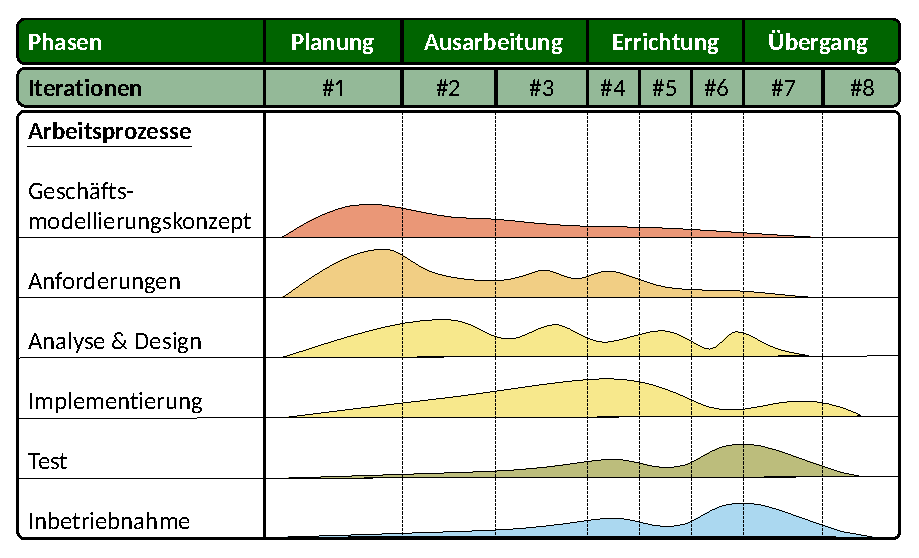
\includegraphics{chapter/chapter_3/rup.eps}
    \caption{Modellierung zum Vorgehen des Rational Unified Process.}
    \label{sec3:model:subsec:conc-model-metho:fig:rup}
\end{figure}

Die Kern-Arbeitsprozesse \enquote{Geschäfts-Modellierungskonzept}, \enquote{Anforderungen} und \enquote{Analyse \& Gestaltung} sind Teil dieses Kapitels und setzen die Methodik für die Bearbeitung der Forschungsziele der Theoriebildungsphase nach Nunamaker um.
Der Arbeitsprozess \enquote{Implementierung} des RUP-Vorgehensmodells entspricht den Forschungszielen der Implementierungsphase nach Nunamaker und wird in \cref{sec4:impl} behandelt.
Der Arbeitsprozess \enquote{Test} des RUP-Vorgehensmodells entspricht den Forschungszielen der Experimentphase nach Nunamaker und wird in \cref{sec5:eval} behandelt. Der Arbeitsprozess \enquote{Inbetriebnahme} wird in dieser Arbeit nicht behandelt. Somit wird jeder konzeptionelle Entwurf und jede Modellierung aus der Perspektive eines Benutzers oder eines Anwendungsfalls und auf Grundlage der Arbeitsprozesse des RUP-Vorgehensmodells entwickelt und im weiteren Verlauf dieser Arbeit unter Verwendung der UML formalisiert. Dabei
ist es Ziel der Modellierung wiederverwendbare Softwarekomponenten zu erstellen, die erweiterbar, konfigurierbar sowie wartbar sind. Die Auswahl der Konzeptions- und Modellierungsmethodiken erfordert eine spezielle Anordnung der Forschungsziele. Diese Anordnung sieht wie folgt aus:
\begin{itemize}
    \item FZ 1.2/TB Erklärbarkeit von MMIR mittels generativer KI
    \item FZ 2.2/TB Integration generativer KI in das GMAF
\end{itemize}
Die Notwendigkeit dieser Anordnung ergibt sich nach der Methodik von Norman \& Draper, in welcher die Modellierung aus der Perspektive eines Benutzers oder eines Anwendungsfalls beginnt. Des Weiteren bauen die ersten Kern-Arbeitsprozesse \enquote{Geschäfts-Modellierungskonzept} und \enquote{Anforderungen} des RUP-Vorgehensmodells auf Anwendungsfällen auf. Somit ist logischer Startpunkt die Erklärbarkeit von MMIR mittels generativer KI.

\FloatBarrier

\subsubsection{Unified Modeling Language}
\label{sec3:model:subsubsec:uml}
Die Unified Modeling Language (UML) \cite{omg-uml} ist eine standardisierte, visuelle Modellierungssprache, die ihre Verwendung in der Softwareentwicklung findet \cite{visual-paradigm-uml}.
UML kann allerdings auch in anderen technischen Bereichen, oder der Geschäftsmodellierung verwendet werden \cite{Kreische2004}.
Die UML hat zum Ziel, komplexe Systeme und deren Prozesse grafisch darzustellen, zu analysieren, zu spezifizieren und zu dokumentieren \cite{visual-paradigm-uml}.
Die UML wurde dazu entwickelt, um die Kommunikation zwischen Softwareentwicklern, Analysten, Designern und anderen involvierten Parteien bzw. Interessensgruppen zu erleichtern \cite{visual-paradigm-uml}.
Um diese Kommunikation zu ermöglichen, bietet die UML eine Vielzahl von Diagrammtypen zur einheitlichen, verständlichen und flexiblen Darstellung von Systemstrukturen- und verhalten.
Folgende Aufzählung umfasst die bekanntesten und am häufigsten verwendeten Diagrammtypen, sowie ihre jeweiligen Aufgaben.
\begin{itemize}
    \item Klassendiagramm: Stellt die simple, statische Struktur eines Systems durch seine Klassen, Attribute, Methoden und deren Beziehungen untereinander dar.
    \item Anwendungsfalldiagramm: Stellt die Interaktion zwischen Akteuren, die Benutzer oder widerum andere Systeme sein können, und dem System dar.
    Zweck ist die Darstellung der für die Akteure verfügbaren Funktionalitäten des Systems.
    \item Sequenzdiagramm: Stellt die Interaktion zwischen Objekten eines Systems in einem zeitlichen Verlauf dar.
    Interaktion geschieht durch das Senden von Nachrichten zwischen den Objekten.
    \item Aktivitätsdiagramm: Stellt den Ablauf von Aktivitäten und Prozessen dar, um den Kontrollfluss innerhalb eines Systems zu visualisieren.
    \item Zustandsdiagramm: Stellt den Lebenszyklus eines Objekts dar und zeigt auf, wie es auf Ereignisse und Zuständsänderungen reagiert.
\end{itemize}
Die wichtigste Eigenschaft der UML ist seine Unabhängigkeit zu spezifischen Technologien, wie z.B. Programmiersprachen \cite{ibm-uml}.
Diese Eigenschaft ermächtigt die UML zur Modellierung verschiedenster Systeme in vielen unterschiedlichen Bereichen.
Bekannte Beispiele sind Softwareanwendungen, Datenbanken und Geschäftsprozesse.
Mittels eines wohl definierten, sowie gepflegten Standards, der durch die OMG \cite{omg} erfolgt und eine einheitliche Sprache für Kommunikation schafft, ermöglicht die UML eine nahtlose Zusammenarbeit zwischen verschiedensten involvierten Gruppen.
Angesichts dieser Eigenschaft ist die Unified Modeling Language ein wertvolles Werkzeug für die Softwaremodellierung- und entwicklung komplexer Systeme.

\clearpage

\subsection[FZ 1.2/TB Erklärbarkeit von MMIR mittels generativer KI]{\texorpdfstring{FZ 1.2/TB Erklärbarkeit von MMIR mittels \\ generativer KI}{FZ 1.2/TB Erklärbarkeit von MMIR mittels generativer KI}}
\label{sec3:model:subsec:fz-explainability}
Dieser Abschnitt befasst sich mit der Modellierung der \enquote{Erklärbarkeit von MMIR mittels generativer KI}.
Dabei werden die in \hyperref[sec2:sota:subsec:fz-explainability]{FZ 1.1/O} identifizierten, offenen Herausforderungen \hyperref[sec2:sota:oi:1.1]{\textbf{OH 1.1}} und \hyperref[sec2:sota:oi:1.2]{\textbf{OH 1.2}} adressiert.
Ziel dieses Abschnitts ist es Konzepte für den Einsatz von Systeme generativer KI für Erklärbarkeit hervorzubringen und Anwendungsfälle zur Interaktion mit selbigen zu identifizieren.
Hierzu wird in \cref{sec3:model:subsubsec:explainability-through-genai} die offene Herausforderung \hyperref[sec2:sota:oi:1.1]{\textbf{OH 1.1}} und in \cref{sec3:model:subsubsec:use-cases} die offene Herausforderung \hyperref[sec2:sota:oi:1.2]{\textbf{OH 1.2}} adressiert.

\subsubsection{Erklärbarkeit durch generative KI}
\label{sec3:model:subsubsec:explainability-through-genai}
In diesem Abschnitt wird die erste offene Herausforderung \hyperref[sec2:sota:oi:1.1]{\textbf{OH 1.1}} adressiert und es werden mögliche Techniken zum Erzeugen von Erklärungen durch generative KI angesprochen.
In \cref{sec2:sota:par:basic-concepts} wurde das Konzept des Prompt Engineering erklärt und eine Reihe an Techniken, sowie dazugehörige Beispiele präsentiert.
Um mit Hilfe von Systemen generativer KI Erklärungen generieren zu können, müssen die Eingaben in ein System möglichst präzise formuliert sein.
Ziel muss es daher sein, mit gezielten und präzise formulierten Eingabeaufforderungen das System so zu instruieren, dass es möglichst genaue Erklärungen generieren kann.
In \cite{zero-shot-reasoners} wurde bereits gezeigt, dass das recht simple Textanhängsel \enquote{Lets think step by step.} einen großen Einfluss auf die Schlussfolgerungen und somit auch die Ausgabe einer generativen KI haben kann.
Es ist daher nicht abwegig anzunehmen, dass eine simple Instruktion, wie z.B. \enquote{Create a coherent textual explanation.} oder \enquote{Create a visual explanation.} einen positiven Einfluss auf erzeugte Texte bzw. Erklärungen haben könnte.
Eine weitere interessante Idee Erklärungen generieren zu lassen, wäre die Methode des Geschichtenerzählens.
Eine beispielhafte Instruktion könnte sein: \enquote{Make up a story.}.
Weitere \enquote{elementare Bausteine} einer Instruktion können dann beispielhafte Erklärungen umfassen, um dem System zu zeigen, welche Art von Erklärung letztlich gewünscht wird, oder die Vorgabe eines unvollständigen Satzes, welcher dann vom System komplementiert wird.

\subsubsection{Anwendungsfälle}
\label{sec3:model:subsubsec:use-cases}
Ein sinnvoller Einsatz von Systemen generativer KI im GMAF zur Erklärung von Graph Codes setzt eine Benutzerschnittstelle mit geeigneten Interaktionsmöglichkeiten voraus.
In diesem Abschnitt wird die zweite offene Herausforderung \hyperref[sec2:sota:oi:1.2]{\textbf{OH 1.2}} adressiert und es werden eine Reihe an Anwendungsfällen aus der Perspektive von Benutzern bzw. Anwendern des GMAF identifiziert und beschrieben.
\cref{sec3:model:subsubsec:use-cases:fig:overview-use-cases} zeigt ein UML-Diagramm zur Übersicht der identifizierten Anwendungsfälle.
\begin{figure}[htb]
    \centering
    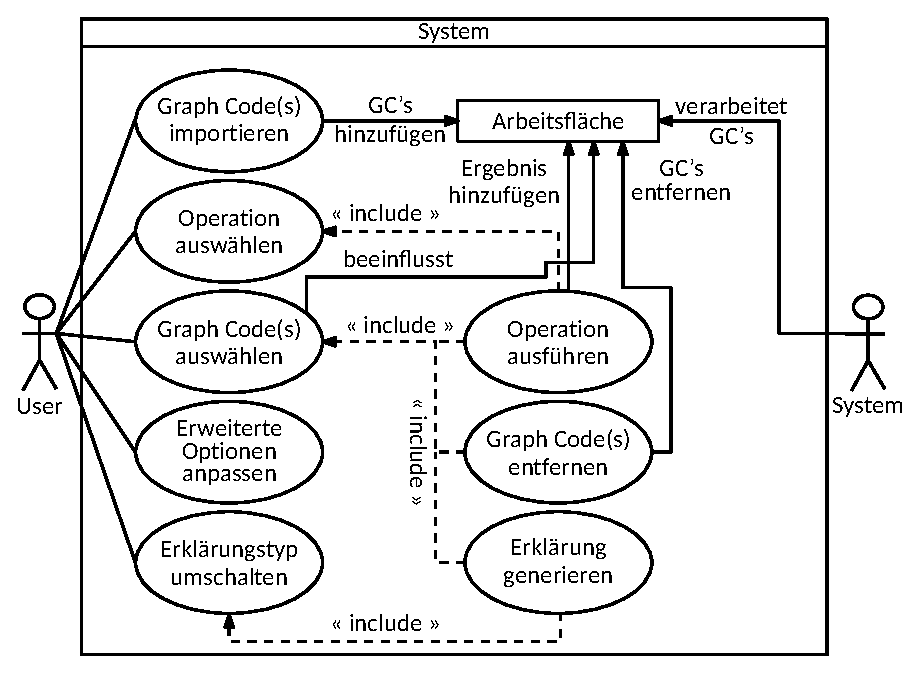
\includegraphics[width=\textwidth]{chapter/chapter_3/uml-explainer-system.eps}
    \caption{Übersicht über alle Anwendungsfälle.}
    \label{sec3:model:subsubsec:use-cases:fig:overview-use-cases}
\end{figure}
\noindent
Diese identifizierten Anwendungsfälle stellen die Basis für weitere Modellierungsvorgehen dar und werden im Laufe dieses Abschnitts weiter ausgeführt.
Weitere Ausführungen umfassen textuelle Beschreibungen, erste Wireframes, die das allgemeine Skelett der Anwendung darstellen sollen, Mechanismen, die die an Anwendungsfällen beteiligten Komponenten identifizieren, sowie Sequenzdiagramme, um die Interaktion zwischen den Objekten bzw. Komponenten eines Systems darzustellen.
Anhand dieser Modellierungsvorgehen werden die Wireframes weiter ausgeführt bzw. ausgebaut.

\paragraph{Textuelle Beschreibungen}
\label{sec3:model:par:textual-desc-use-cases}
In diesem Abschnitt werden die in \cref{sec3:model:subsubsec:use-cases:fig:overview-use-cases} dargestellten Anwendungsfälle detailliert beschrieben.
Diese detaillierte Beschreibung umfasst jeweils eine Beschreibung der Aufgabe des Anwendungsfalles, die Akteure, die an diesem Anwendungsfall beteiligt sind, die Vorbedingungen, die vor dem Anwendungsfall gelten, einen Ablauf an Schritten zum Durchführen des Anwendungsfalls und schlussendlich die Nachbedinungen, die jeweils nach dem Anwendungsfall gelten.

\begin{usecase}{UC-1.1 Graph Code(s) importieren}
\label{sec3:model:uc-1.1}
    \desc{
        Benutzer klicken in der Arbeitsfläche einen Knopf \enquote{Select Graph Code(s)}.
        Daraufhin öffnet sich ein Filechooser, in welchem Benutzer eine Auswahl von einem oder mehrerer Graph Code Datei(en) treffen können.
        Die ausgewählten Graph Code Datei(en) werden einer Liste in der Arbeitsfläche hinzugefügt und angezeigt.
    }
    \tcbline
    \actors{Benutzer, System}
    \tcbline
    \pre{Keine.}
    \tcbline
    \mainflow{
        \item System zeigt eine Liste in der Arbeitsfläche an.
        \item Benutzer klickt Knopf \enquote{Select Graph Code(s).}
        \item System zeigt Filechooser an.
        \item Benutzer wählt ein oder mehrere Graph Code Datei(en) aus.
        \item System fügt Graph Code Datei(en) der Liste in der Arbeitsfläche zu.
    }
    \tcbline
    \post{Graph Code Datei(en) sind der Liste in der Arbeitsfläche hinzugefügt worden.}
\end{usecase}

\begin{usecase}{UC-1.2 Graph Code(s) entfernen}
\label{sec3:model:uc-1.2}
    \desc{
        Benutzer wählen aus der Liste in der Arbeitsfläche ein oder mehrere Graph Code Datei(en) aus und können über einen Knopf \enquote{Remove selected Graph Code(s)} diese Graph Codes aus der Liste und somit der Arbeitsfläche entfernen.
    }
    \tcbline
    \actors{Benutzer, System}
    \tcbline
    \pre{
        \begin{itemize}
            \item Liste enthält ein oder mehrere Graph Code(s).
            \item Benutzer haben ein oder mehrere Graph Code(s) ausgewählt.
        \end{itemize}
    }
    \tcbline
    \mainflow{
        \item System zeigt eine Liste an Graph Codes in der Arbeitsfläche an.
        \item Benutzer wählt ein oder mehrere Graph Code(s) aus.
        \item Benutzer klickt auf Knopf \enquote{Remove selected Graph Code(s).}
        \item System entfernt ausgewählte Graph Codes aus der Liste in der Arbeitsfläche.
    }
    \tcbline
    \post{Ausgewählte Graph Code Datei(en) sind aus der Liste in der Arbeitsfläche entfernt worden.}
\end{usecase}

\begin{usecase}{UC-1.3 Graph Code(s) auswählen}
\label{sec3:model:uc-1.3}
    \desc{
        Benutzer wählen aus der Liste in der Arbeitsfläche ein oder mehrere Graph Code Datei(en) aus.
        Die Auswahl von Graph Code Dateien dient als Grundlage für Anwendungsfälle, wie \hyperref[sec3:model:uc-1.2]{UC-1.2}, \hyperref[sec3:model:uc-1.5]{UC-1.5} oder \hyperref[sec3:model:uc-1.8]{UC-1.8}.
    }
    \tcbline
    \actors{Benutzer, System}
    \tcbline
    \pre{
        Liste enthält ein oder mehrere Graph Code(s) zum Auswählen.
    }
    \tcbline
    \mainflow{
        \item System zeigt eine Liste an Graph Code(s) in der Arbeitsfläche an.
        \item Benutzer wählen ein oder mehrere Graph Code(s) an.
    }
    \tcbline
    \post{Keine.}
\end{usecase}

\begin{usecase}{UC-1.4 Operation auswählen}
\label{sec3:model:uc-1.4}
    \desc{
        Benutzer wählen aus einem Feld eine auszuführende Operation aus.
        Verfügbare Optionen sind: Vereinigung, Subtraktion, Gemeinsamkeiten, Unterschiede.
        Das Auswählen einer Operation ist die Vorbedingung für den Anwendungsfall \hyperref[sec3:model:uc-1.5]{UC-1.5}, dem Ausführen einer Operation.
    }
    \tcbline
    \actors{Benutzer, System}
    \tcbline
    \pre{Keine.}
    \tcbline
    \mainflow{
        \item System bietet in einem Feld eine Reihe an auszuwählenden Operationen.
        \item Benutzer wählt eine Operation aus.
    }
    \tcbline
    \post{Keine.}
\end{usecase}

\begin{usecase}{UC-1.5 Operation ausführen}
\label{sec3:model:uc-1.5}
    \desc{
        Benutzer klicken auf den Knopf \enquote{Execute}, um die vorher ausgewählte Operation auf den in der Arbeitsfläche ausgewählten Graph Code Datei(en) auszuführen.
        Die vorher ausgewählte Operation wird daraufhin auf den ausgewählten Graph Code Datei(en) ausgeführt.
    }
    \tcbline
    \actors{Benutzer, System}
    \tcbline
    \pre{
        \begin{itemize}
            \item Operation in der Arbeitsfläche ausgewählt.
            \item In der Arbeitsfläche wurden Graph Code Datei(en) ausgewählt.
        \end{itemize}
    }
    \tcbline
    \mainflow{
        \item Benutzer klickt auf Knopf \enquote{Execute}.
        \item System führt vorher ausgewählte Operation auf den ausgewählten Graph Code Datei(en) aus.
    }
    \tcbline
    \post{Erfolgreich ausgeführte Operation auf ausgewählten Graph Code(s).}
\end{usecase}

\begin{usecase}{UC-1.6 Erklärungstyp umschalten}
\label{sec3:model:uc-1.6}
    \desc{
        Benutzer wählen in der Arbeitsfläche über Knöpfe \enquote{Image} oder \enquote{Text} den Typ der Erklärung aus.
        Anhand der ausgewählten Erklärung wird die Benutzerschnittstelle in der Arbeitsfläche für den jeweiligen Erklärungstyp umgeschaltet.
    }
    \tcbline
    \actors{Benutzer, System}
    \tcbline
    \pre{Keine.}
    \tcbline
    \mainflow{
        \item Benutzer wählen über die Knöpfe \enquote{Image} oder \enquote{Text} den Typ der Erklärung aus.
        \item System schaltet auf für Typ spezifische Benutzerschnittstelle um.
    }
    \tcbline
    \post{Benutzerschnittstelle für spezifischen Erklärungstyp umgeschaltet.}
\end{usecase}

\begin{usecase}{UC-1.7 Erweiterte Optionen anpassen}
\label{sec3:model:uc-1.7}
    \desc{
        Benutzer passen in einem dafür vorgesehenen Feld erweiterte Optionen für den Endpunkt, der für die zu generierende Erklärung zuständig ist, an.
        Die anpassbaren Optionen sind abhängig vom jeweiligen Endpunkt bzw. Erklärungstypen.
    }
    \tcbline
    \actors{Benutzer, System}
    \tcbline
    \pre{Keine.}
    \tcbline
    \mainflow{
        \item System bietet, abhängig vom Endpunkt bzw. Erklärungstypen, eine Reihe an anpassbaren Optionen an.
        \item Benutzer passen Optionen nach eigenen Bedürfnissen an.
    }
    \tcbline
    \post{Keine.}
\end{usecase}

\begin{usecase}{UC-1.8 Erklärung generieren}
\label{sec3:model:uc-1.8}
    \desc{
        Benutzer klicken auf einen Knopf \enquote{Generate ...}, um eine Erklärung für eine zuvor ausgewählte Graph Code Datei zu generieren.
        Die generierte Erklärung ist abhängig vom zuvor gewählten Endpunkt bzw. Erklärungstypen.
    }
    \tcbline
    \actors{Benutzer, System}
    \tcbline
    \pre{Graph Code Datei wurde ausgewählt.}
    \tcbline
    \mainflow{
        \item Benutzer klickt auf Knopf \enquote{Generate ...}
        \item System lässt durch Endpunkt Erklärung generieren.
        \item System zeigt Erklärung in einem dafür vorgesehenen Bereich der Benuzterschnittstelle an.
    }
    \tcbline
    \post{Keine.}
    \tcbline
    % Hier im Branchflow zwischen Image und Text differenzieren.
    \branchflow{
        \setcounter{enumi}{2}
        \item[\number\value{enumi}.a] Endpunkt für \enquote{Image} generiert eine visuelle Erklärung bzw. ein Bild.
        \item[\number\value{enumi}.b] Endpunkt für \enquote{Text} generiert eine textuelle Erklärung.
    }
\end{usecase}

\paragraph{Wireframe für die Interaktion mit Graph Codes}
\label{sec3:model:par:wireframe}
Auf Basis der Anwendungsfälle und den textuellen Beschreibungen dieser, wird in diesem Abschnitt ein Wireframe, sprich ein Konzept für eine Benutzerschnittstelle, vorgestellt.
\cref{sec3:model:par:wireframe:fig:stage-1} zeigt eine erste Ausführung eines Wireframes, welches die Grundbereiche und somit das Skelett der Benutzerschnittstelle darstellen soll.

\begin{figure}[htb]
    \centering
    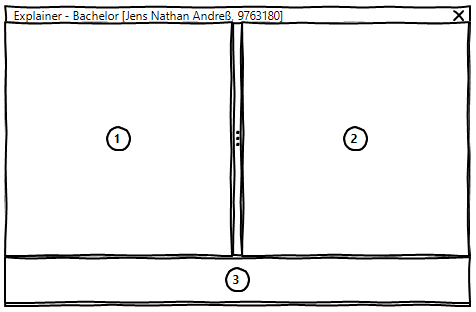
\includegraphics{chapter/chapter_3/wireframe-stage-1.png}
    \caption{Wireframe für die Grundbereiche der Benutzerschnittstelle.}
    \label{sec3:model:par:wireframe:fig:stage-1}
\end{figure}

In dieser Abbildung sind drei Grundbereiche zu erkennen, die im Folgenden genauer beschrieben werden:
\begin{enumerate}
    \item[\circitem{1}] ist der Bereich der Arbeitsfläche, in der die Bearbeitung von Graph Code Dateien stattfindet.
    Bearbeitungen von Graph Codes umfassen das Importieren, Auswählen und Entfernen von Graph Code Dateien, sowie das Auswählen und Ausführen von Operationen auf Graph Code Dateien.
    \item[\circitem{2}] ist der Bereich der Arbeitsfläche, in der Benutzer Erklärungen generieren können.
    Benutzer können hier zwischen unterschiedlichen Typen an Erklärungen hin und her schalten.
    \item[\circitem{3}] ist eine Konsole, in der alle wichtigen Informationen über Aktionen und Prozesse festgehalten werden.
\end{enumerate}
Anhand der Anwendungsfälle \hyperref[sec3:model:uc-1.1]{UC-1.1} bis \hyperref[sec3:model:uc-1.5]{UC-1.5} können in der linken Arbeitsfläche, die der Bearbeitung von Graph Codes dienen soll, wichtige Komponenten in der Benutzerschnittstelle identifiziert werden.
Analog können anhand der Anwendungsfälle \hyperref[sec3:model:uc-1.6]{UC-1.6} bis \hyperref[sec3:model:uc-1.8]{UC-1.8} in der rechten Arbeitsfläche, die sich der Erklärung von Graph Code Dateien widmet, weitere wichtige Komponenten in der Benutzerschnittstelle identifiziert werden.
\cref{sec3:model:par:wireframe:fig:stage-2+3} zeigt die linke und rechte Arbeitsfläche mit diesen neuen Komponenten in jeweils einem partiellen Wireframe.

\begin{figure}[htb]
    \centering
    \begin{minipage}[b]{.5\textwidth}
        \centering
        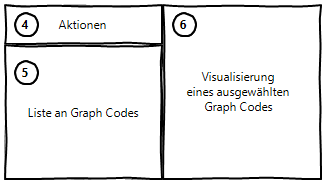
\includegraphics[width=\textwidth]{chapter/chapter_3/wireframe-stage-2.png}
    \end{minipage}%
    \begin{minipage}[t]{.5\textwidth}
        \centering
        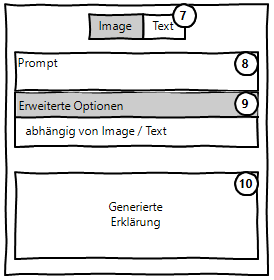
\includegraphics[width=0.9\textwidth]{chapter/chapter_3/wireframe-stage-3.png}
    \end{minipage}
    \caption{Wireframe für den linken Arbeitsbereich (links) und den rechten Arbeitsbereich (rechts) der Benutzerschnittstelle.}
    \label{sec3:model:par:wireframe:fig:stage-2+3}
\end{figure}

Diese neuen Komponenten werden im Folgenden genauer beschrieben:
\begin{enumerate}
    \item[\circitem{4}] ist der Aktionsbereich, in welchem Interaktionsmöglichkeiten, wie das Importieren und Entfernen von Graph Codes in die Arbeitsfläche eingebunden werden.
    Des Weiteren werden in diesem Aktionsbereich auch Interaktionsmöglichkeiten für die Auswahl und das Ausführen von Operationen auf den zuvor in der Arbeitsfläche ausgewählten Graph Code Dateien eingebunden.
    \item[\circitem{5}] ist der Bereich in der Benutzerschnittstelle, in der die Graph Code Dateien in einer Liste dargestellt werden.
    Diese Liste ist die Voraussetzung für Anwendungsfälle \hyperref[sec3:model:uc-1.2]{UC-1.2}, \hyperref[sec3:model:uc-1.3]{UC-1.3}, \hyperref[sec3:model:uc-1.5]{UC-1.5} und \hyperref[sec3:model:uc-1.8]{UC-1.8}.
    \item[\circitem{6}] ist der Bereich der Benutzerschnittstelle, in der ausgewählte Graph Code Datei(en) in einer geeigneten Form visualisiert werden.
    Da Graph Codes quadratische Matrizen sind, eignet sich für die visuelle Form der Darstellung eine Tabelle.
    \item[\circitem{7}] sind die Knöpfe, mit welchen Benutzer zwischen den Benutzerschnittstellen für die jeweiligen Erklärungstypen umschalten können.
    \item[\circitem{8}] ist die Prompt, die später über den entsprechenden Endpunkt in das System generativer KI übermittelt werden soll.
    \item[\circitem{9}] zeigt erweiterte anpassbare Optionen für den jeweiligen Endpunkt.
    \item[\circitem{10}] ist der Bereich, in welchem das Endergebnis der Anfrage an das System generativer KI dargestellt wird.
\end{enumerate}
Zusammengeführt ergeben diese partiellen Wireframes ein ganzes Wireframe, welches in \cref{sec3:model:par:wireframe:fig:complete-stage} abgebildet ist und die komplette Benutzerschnittstelle darstellt.

\begin{figure}[htb]
    \centering
    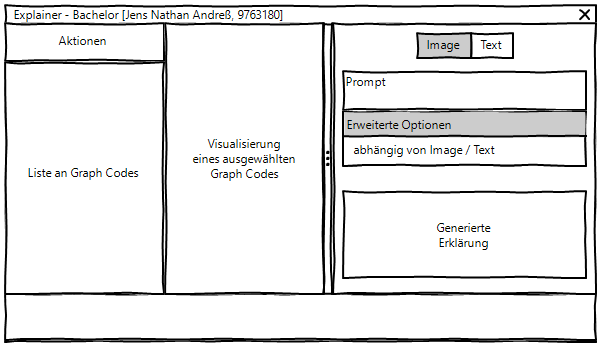
\includegraphics[width=\textwidth]{chapter/chapter_3/wireframe-complete-stage.png}
    \caption{Komplettes Wireframe für die Benutzerschnittstelle.}
    \label{sec3:model:par:wireframe:fig:complete-stage}
\end{figure}
Die in diesem Abschnitt dargestellten Wireframes bilden die Struktur der Benutzerschnittstelle und werden im weiteren Verlauf dieser Arbeit in \hyperref[sec4:impl:subsec:fz-explainability]{FZ 1.3/I} im Rahmen einer prototypischen Implementierung untersucht.
Im weiteren Verlauf diese Forschungsziels werden nun mittels Mechanismen die an Anwendungsfällen beteiligten Komponenten identifiziert, sowie deren Zusammenspiel in einer kurzen Erklärung angerissen.
Aufbauend auf diesen Erkenntnissen wird weiter mittels Sequenzdiagrammen das Verhalten zwischen diesen Komponenten untersucht und festgehalten.

\FloatBarrier

\paragraph{Mechanismen}
\label{sec3:model:par:mechanism-use-cases}
Ein Mechanismus ist ein partielles Klassendiagramm, das die Menge aller Klassen, von denen Instanzen in irgendeinem Objektdiagramm für einen Anwendungsfall vorkommen, darstellt.
Mechanismen haben somit zum Ziel, die an einem Anwendungsfall beteiligten Objekte bzw. Klassen zu identifizieren und darzustellen.
In einem Mechanismus wird der Anwendungsfall selbst gestrichelt dargestellt und die mit diesem Anwendungsfall assoziierten Klassen werden ebenfalls durch gestrichelte Linien mit dem Anwendungsfall verbunden.
Im weiteren Verlauf dieses Kapitels werden die in Mechanismen identifizierten Klassen zusammen mit den in den Anwendungsfällen beschriebenen Abläufen die Basis für Sequenz- und Klassendiagramme bilden.
Im weiteren Verlauf dieses Abschnitts werden nun für ausgewählte Anwendungsfälle Mechanismen erstellt.

\begin{figure}[htb]
    \centering
    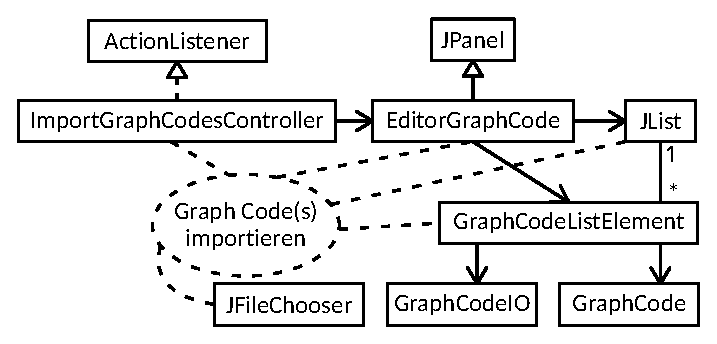
\includegraphics{chapter/chapter_3/mechanisms/mechanism-uc-1.1.eps}
    \caption{Mechanismus für den Anwendungsfall \hyperref[sec3:model:uc-1.1]{UC-1.1}.}
    \label{sec3:model:par:mechanism-use-cases:fig:mech-uc-1.1}
\end{figure}
\cref{sec3:model:par:mechanism-use-cases:fig:mech-uc-1.1} zeigt den Mechanismus für den Anwendungsfall \hyperref[sec3:model:uc-1.1]{UC-1.1}.
Sobald der Anwendungsfall \hyperref[sec3:model:uc-1.1]{UC-1.1} beginnt, benötigt es eine Komponente, die die in diesem Anwendungsfall enthaltenen Subaktionen steuert.
Diese Aufgabe übernimmt die Komponente \textit{ImportGraphCodesController}.
Da das Importieren von Graph Codes das Auswählen der jeweiligen Graph Code Datei(en) erfordert, benötigt es einen Auswahldialog \textit{JFileChooser}.
Die nun durch den Benutzer ausgewählten Dateien werden einer Liste in der Arbeitsfläche hinzugefügt.
Genauer ist diese Arbeitsfläche die linke Arbeitsfläche (siehe \cref{sec3:model:par:wireframe:fig:stage-1} \circitem{1}) und wird in diesem Diagramm durch \textit{EditorGraphCode} dargestellt.
Diese Arbeitsfläche zeigt eine (1) Liste \textit{JList} (siehe \cref{sec3:model:par:wireframe:fig:stage-2+3} \circitem{5}), welcher beliebig viele (*) Graph Codes \textit{GraphCodeListElement} hinzugefügt werden können.

\begin{figure}[htb]
    \centering
    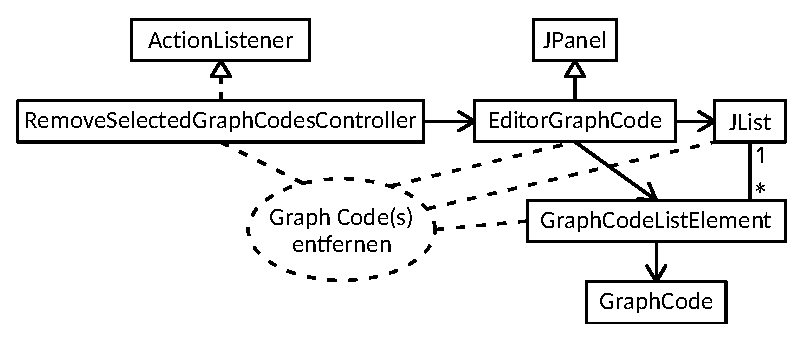
\includegraphics{chapter/chapter_3/mechanisms/mechanism-uc-1.2.eps}
    \caption{Mechanismus für den Anwendungsfall \hyperref[sec3:model:uc-1.2]{UC-1.2}.}
    \label{sec3:model:par:mechanism-use-cases:fig:mech-uc-1.2}
\end{figure}
\cref{sec3:model:par:mechanism-use-cases:fig:mech-uc-1.2} zeigt den Mechanismus für den Anwendungsfall \hyperref[sec3:model:uc-1.2]{UC-1.2}.
Der Mechanismus für den Anwendungsfall \hyperref[sec3:model:uc-1.2]{UC-1.2} ist sehr ähnlich im Vergleich zum Mechanismus für den Anwendungsfall \hyperref[sec3:model:uc-1.2]{UC-1.2}.
Einzig erwähnenswert ist die Komponente \textit{RemoveSelectedGraphCodesController}, die die notwendigen Subaktionen zum Entfernen von Graph Codes steuert.

\begin{figure}[htb]
    \centering
    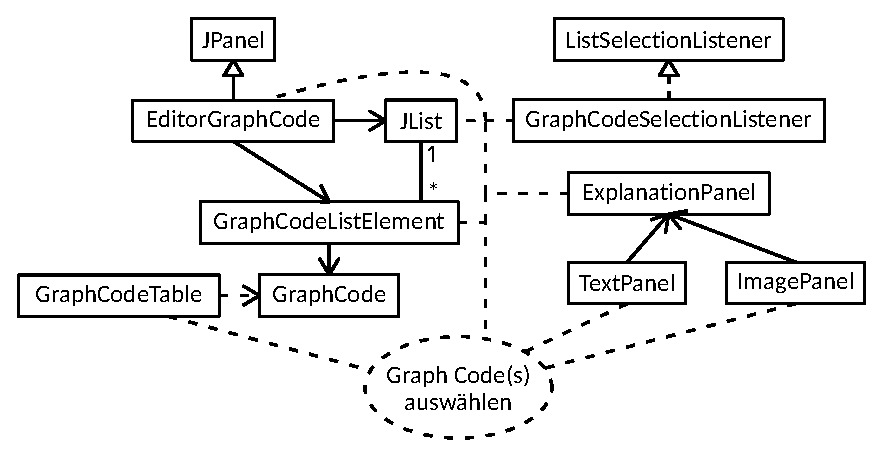
\includegraphics{chapter/chapter_3/mechanisms/mechanism-uc-1.3.eps}
    \caption{Mechanismus für den Anwendungsfall \hyperref[sec3:model:uc-1.3]{UC-1.3}.}
    \label{sec3:model:par:mechanism-use-cases:fig:mech-uc-1.3}
\end{figure}

\cref{sec3:model:par:mechanism-use-cases:fig:mech-uc-1.3} zeigt den Mechanismus für den Anwendungsfall \hyperref[sec3:model:uc-1.3]{UC-1.3}.
Der Anwendungsfall \hyperref[sec3:model:uc-1.3]{UC-1.3} beginnt mit der Auswahl von Graph Code(s).
Das Auswählen von Graph Codes beeinflusst mehrere Komponenten in der gesamten Benutzerschnittstelle.
Die Aktionen zur Einflussnahme auf diese Komponenten werden durch die Komponente \textit{GraphCodeSelectionListener} gesteuert.
Beeinflusste Komponenten umfassen die Komponente \textit{GraphCodeTable} (siehe \cref{sec3:model:par:wireframe:fig:stage-2+3} \circitem{6}), sowie die Komponente \textit{ExplanationPanel} (siehe \cref{sec3:model:par:wireframe:fig:stage-2+3} \circitem{2}), in der Benutzer zwischen Erklärungstypen umschalten können.
Die Komponenten \textit{ImagePanel} und \textit{TextPanel} sind die für die Erklärungstypen spezifischen Benutzerschnittstellen, und können durch \cref{sec3:model:par:wireframe:fig:stage-2+3} \circitem{7} umhergeschaltet werden.

% Mechanismus zu Anwendungsfall 1.5, und Mechanismus hier als Basis für die spätere Diskussion und den Aspekt der Operationsverkettung...
\begin{figure}[htb]
    \centering
    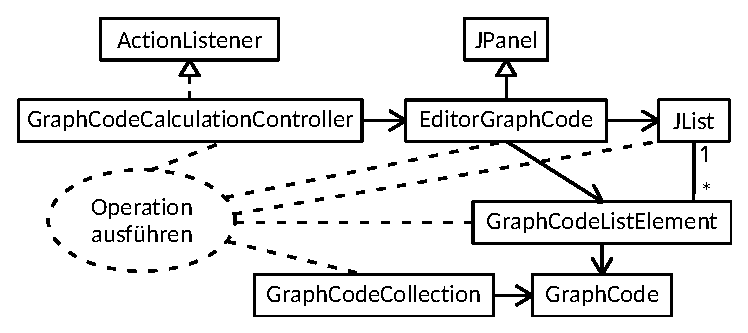
\includegraphics{chapter/chapter_3/mechanisms/mechanism-uc-1.5.eps}
    \caption{Mechanismus für den Anwendungsfall \hyperref[sec3:model:uc-1.5]{UC-1.5}.}
    \label{sec3:model:par:mechanism-use-cases:fig:mech-uc-1.5}
\end{figure}

\cref{sec3:model:par:mechanism-use-cases:fig:mech-uc-1.5} zeigt den Mechanismus für den Anwendungsfall \hyperref[sec3:model:uc-1.5]{UC-1.5}.
Der Anwendungsfall \hyperref[sec3:model:uc-1.5]{UC-1.5} \enquote{Operation ausführen} beginnt durch das Klicken des Knopfes \enquote{Execute}.
Die an diesem Anwendungsfall beteiligten Aktionen werden durch die Komponente \textit{GraphCodeCalculationController} gesteuert und geleitet.
Dies beinhaltet auch das Differenzieren der in Anwendungsfall \hyperref[sec3:model:uc-1.4]{UC-1.4} zuvor ausgewählten Operation.
Diese Operation kann die \textit{Vereinigung (Union)}, \textit{relative Differenz / Unterschied bzw. Subtraktion}, \textit{Gemeinsamkeiten (Similarities)} oder \textit{Unterschiede (Differences) }zwischen mehreren Graph Codes sein.
Besonders hierbei ist die \textit{Subtraktion}, die nur auf zwei Graph Codes angewandt werden kann.
Die Algorithmen zur Berechnung der Operationen der \textit{Vereinigung} von mehreren Graph Codes, sowie der \textit{Subtraktion} zweier Graph Codes werden bereits durch die Komponente \textit{GraphCodeCollection} bereitgestellt.
Im Folgenden werden Konzepte für die weiteren Operationen \textit{Gemeinsamkeiten} und \textit{Unterschiede} in Form von Pseudoalgorithmen vorgestellt, und es werden die an diesen Operationen beteiligten Komponenten, ihre Aufgaben, sowie durchzuführende Schritte beschrieben.

\begin{algorithm}[htb]
\caption{Berechne Gemeinsamkeiten}
\label{sec3:model:par:mechanism-use-cases:alg:sim}
\begin{algorithmic}[1]
\Require{Liste an Graph Codes: gcs}
\Ensure{Graph Code}
\Function{GetSimilarities}{$\text{gcs}$}
    %\State Graph Code für Gemeinsamkeiten (sim) $\gets$ new GraphCode
    %\State Vereinigung von Graph Codes (union) $\gets$ getUnion(gcs)
    %\State Vokabular von union (unionDic) $\gets$ new Vector(Vokabular von union)
    \State sim $\gets$ new GraphCode
    \State union $\gets$ getUnion(gcs)
    \State unionDic $\gets$ new Vector(union.getDictionary())
    \For{gc in gcs}
        \State \shortstack[l]{Entferne alle Elemente aus unionDic, \\die nicht im Vokabular von gc enthalten sind}
    \EndFor
    \State dictionary $\gets$ new Vector(unionDic)
    \State sim.setDictionary(dictionary)
    
    \For{gci in gcs}
        \For{s in dictionary}
            \For{t in dictionary}
                \State $\text{i} \gets \text{gci.getEdgeValueForTerms}(\text{s}, \text{t})$
                \State $\text{sim.setValueForTerms}(\text{s}, \text{t}, \text{i})$
            \EndFor
        \EndFor
    \EndFor
    \State \textbf{return} $\text{sim}$
\EndFunction
\end{algorithmic}
\end{algorithm}

\cref{sec3:model:par:mechanism-use-cases:alg:sim} zeigt einen Pseudoalgorithmus für die Operation \textit{Gemeinsamkeiten}.
Diese Algorithmus nimmt als Eingabe eine Liste an Graph Codes und gibt als Ergebnis einen Graph Code zurück.
Der Algorithmus kann in drei Bereiche unterteilt werden: \textit{Vorbereitung}, \textit{Berechnung} und \textit{Verwertung}.
Der Bereich \textit{Vorbereitung} umfasst die Zeilen 2 bis 4.
In diesem Bereich wird das Ergebnis als Objekt zum ersten Mal initialisiert.
Weiterhin wird die Vereinigung aller Graph Codes aus der Eingabe der Funktion mit der Funktion getUnion, welche durch die Komponente \textit{GraphCodeCollection} bereitgestellt wird, berechnet.
Ergebnis dieser Vereinigung ist wiederum ein Graph Code, dessen Vokabular zuletzt für die weitere Berechnung in den folgenden Bereichen aufbereitet wird.
Der zweite Bereich \textit{Berechnung} umfasst die Zeilen 5 bis 6.
In diesem Bereich wird das Vokabular der Vereinigung (unionDic) mit dem Vokabular aller Graph Codes aus der Eingabe miteinander verglichen und es werden alle Merkmale aus unionDic, die nicht in irgendeinem Vokabular eines Graph Codes aus der Eingabe vorkommen, entfernt.
Übrig bleiben die Merkmale, die in jedem Graph Code aus der Eingabe vorkommen.
Der dritte Bereich \textit{Verwertung} umfasst die übrigen Zeilen 7 bis 14.
Dem Objekte sim, welches das Ergebnis repräsentiert, wird das Vokabular unionDic gesetzt.
Im weiteren Verlauf wird für jeden Graph Code zeilen- und spaltenweise der Wert für ein Paar aus Merkmalen in der Adjanzenzmatrix bestimmt und dieser Wert in der Matrix des Ergebnisses eingetragen.
Schlussendlich wird das Ergebnis als Ausgabe zurückgegeben.
% comment-soigner u. csm katze allein lassen
In \cref{sec3:model:par:mechanism-use-cases:fig:gc1-2-similarities} wird die beispielhafte Berechnung der Gemeinsamkeiten zweier Graph Codes dargestellt.

\begin{figure}[!ht]
  \centering
  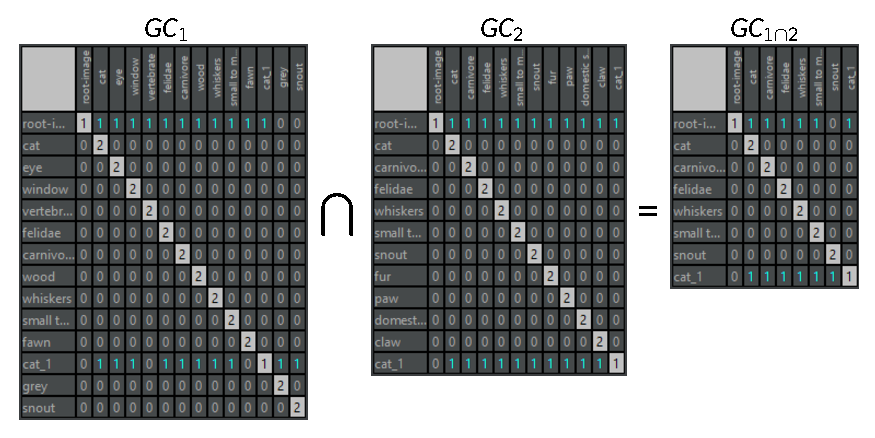
\includegraphics{chapter/chapter_3/algorithms/gc1-2-similarities-ex}
  \caption{Beispielhafte Visualisierung für die Berechnung der Gemeinsamkeiten zweier Graph Codes $GC_1$ und $GC_2$.}
  \label{sec3:model:par:mechanism-use-cases:fig:gc1-2-similarities}
\end{figure}

\begin{algorithm}[htb]
\caption{Berechne Unterschiede}
\label{sec3:model:par:mechanism-use-cases:alg:dif}
\begin{algorithmic}[1]
\Function{GetDifferences}{$\text{gcs}$}
    %\State Graph Code für Gemeinsamkeiten (sim) $\gets$ new GraphCode
    %\State Vereinigung von Graph Codes (union) $\gets$ getUnion(gcs)
    %\State Vokabular von union (unionDic) $\gets$ new Vector(Vokabular von union)
    \State diff $\gets$ new GraphCode
    \State union $\gets$ getUnion(gcs)
    \State unionDic $\gets$ new Vector(union.getDictionary())
    \For{gc in gcs}
        \State \shortstack[l]{Entferne alle Elemente aus unionDic, \\die nicht im Vokabular von gc enthalten sind}
    \EndFor
    
    \State \shortstack[l]{Alle Merkmale bestimmen, die im Vokabular der Vereinigung union,\\ aber nicht im Vokabular unionDic enthalten sind.}
    \State dictionary $\gets$ new Vector(unionDic)
    \State diff.setDictionary(dictionary)
    
    \For{gci in gcs}
        \For{s in dictionary}
            \For{t in dictionary}
                \State $\text{i} \gets \text{gci.getEdgeValueForTerms}(\text{s}, \text{t})$
                \State $\text{diff.setValueForTerms}(\text{s}, \text{t}, \text{i})$
            \EndFor
        \EndFor
    \EndFor
    \State \textbf{return} $\text{diff}$
\EndFunction
\end{algorithmic}
\end{algorithm}

\cref{sec3:model:par:mechanism-use-cases:alg:dif} zeigt einen Pseudoalgorithmus für die Operation \textit{Unterschiede}.
Dieser Algorithmus ist sehr ähnlich zum \cref{sec3:model:par:mechanism-use-cases:alg:sim} und nimmt ebenfalls eine Liste an Graph Codes und gibt als Ergebnis einen Graph Code zurück.
Zudem kann dieser Algorithmus ebenfalls in die gleichen Bereiche unterteilt werden.
Mehr noch sind die Bereiche \textit{Vorbereitung} (Zeile 2 bis 4) und \textit{Verwertung} (Zeile 10 bis 15) identisch und Unterschiede in den Algorithmen bestehen nur im Bereich \textit{Berechnung} (Zeile 6 - 7).
Genauer besteht der einzige Unterschied im Vergleich zum \cref{sec3:model:par:mechanism-use-cases:alg:sim}, dass unterschiedliche Merkmale in mehreren Graph Codes das Gegenteil der gemeinsamen Merkmale in mehreren Graph Codes ist.
In \cref{sec3:model:par:mechanism-use-cases:fig:gc1-2-differences} wird die beispielhafte Berechnung der Unterschiede zweier Graph Codes dargestellt.

\begin{figure}[!ht]
  \centering
  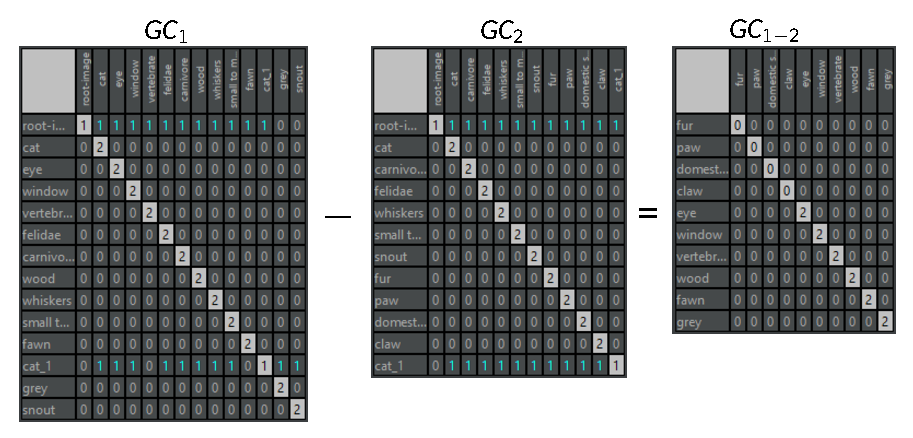
\includegraphics{chapter/chapter_3/algorithms/gc1-2-differences-ex}
  \caption{Beispielhafte Visualisierung für die Berechnung der symmetrische Differenz bzw. Unterschiede zweier Graph Codes $GC_1$ und $GC_2$.}
  \label{sec3:model:par:mechanism-use-cases:fig:gc1-2-differences}
\end{figure}

Zusammengefasst und einfacher ausgedrückt wird in der Operation \textit{Gemeinsamkeiten} die Schnittmenge aller Vokabulare von Graph Codes, welche wiederum nur Mengen von Merkmalen sind, gebildet.
Analog wird in der Operation \textit{Unterschiede} die symmetrische Differenz aller Vokabular von Graph Codes gebildet, welches dem Gegenteil der Schnittmenge aller Vokabulare von Graph Codes entspricht.
Dies unterscheidet die Operation \textit{Unterschiede} von der durch die Komponente \textit{GraphCodeCollection} bereitgestellten Operation \textit{Subtraktion}, welche nur die relative Differenz zweier Graph Codes bildet.

\FloatBarrier

\paragraph{Sequenzdiagramme}
\label{sec3:model:par:seq-use-cases}
Sequenzdiagramme modellieren den konkreten zeitlichen Verlauf von mitunter komplexen Operationen in einem Klassenmodell unter Einbeziehung der in diesen Operationen beteiligten Objekten.
Die in einer Operation beteiligten Objekte werden dabei am oberen Rand des Diagramms als ein Rechteck mit einer gestrichelten vertikalen Linie dargestellt.
Diese gestrichelte vertikale Linie wird als \textit{Lebenslinie} bezeichnet und symbolisiert die Lebenszeit eines Objektes, welche von oben nach unter voranschreitet.
Interaktionen zwischen Objekten, wie z.B. dem Aufrufen einer Operation eines Objektes durch ein anderes Objekt, geschehen durch das Senden von Nachrichten zwischen diesen.
Die gängigsten Formen von Nachrichten sind:

\begin{figure}[htb]
    \centering
    \begin{subfigure}{.25\textwidth}
        \centering
        \tikz{
            \begin{umlseqdiag}
                \umlobject[x=0,fill=white]{A}
                \umlobject[x=1,fill=white]{B}

                \begin{umlcall}{A}{B}
                \end{umlcall}
            \end{umlseqdiag}
        }
        \caption{}
        \label{sec3:model:par:seq-use-cases:subfig:sync-message}
    \end{subfigure}%
    \begin{subfigure}{.25\textwidth}
        \centering
        \tikz{
            \begin{umlseqdiag}
                \umlobject[x=0,fill=white]{A}
                \umlobject[x=1,fill=white]{B}

                \begin{umlcall}[type=asynchron]{A}{B}
                \end{umlcall}
            \end{umlseqdiag}
        }
        \caption{}
        \label{sec3:model:par:seq-use-cases:subfig:async-message}
    \end{subfigure}%
    \begin{subfigure}{.25\textwidth}
        \centering
        \tikz{
            \begin{umlseqdiag}
                \umlobject[x=0,fill=white]{A}
                \umlobject[x=3,fill=white]{B}

                \begin{umlcall}[op={Nachricht},return={Antwort}]{A}{B}
                \end{umlcall}
            \end{umlseqdiag}
        }
        \caption{}
        \label{sec3:model:par:seq-use-cases:subfig:return-message}
    \end{subfigure}%
    \begin{subfigure}{.25\textwidth}
        \centering
        \tikz{
            \begin{umlseqdiag}
                \umlobject[fill=white]{A}

                \begin{umlcallself}{A}
                \end{umlcallself}
            \end{umlseqdiag}
        }
        \caption{}
        \label{sec3:model:par:seq-use-cases:subfig:selfcall}
    \end{subfigure}
    \caption{(i) Synchrone Nachricht, (ii) Asynchrone Nachricht, (iii) Antwort auf Nachricht, (iv) Selbstdelegation / Selbstaufruf.}
    \label{fig:test}
\end{figure}

\begin{enumerate}[label=(\roman{enumi})]
    \item \textit{Synchrone Nachrichten} werden durch einen geschlossenen, gefüllten Pfeil \tikz{ \draw[-{Triangle[angle=90:5pt,length=4mm,fill=black]}] (0,0) -- (0.7,0) {}; } dargestellt.
    Eine synchrone Nachricht repräsentiert einen direkten Aufruf einer Operation vom Dienstnutzenden (Sender) zum Dienstleistenden (Empfänger).
    Eine wichtige Eigenschaft, die diesem Nachrichtentyp seinen Namen verleiht ist, dass der Sender auf die Antwort seiner Nachricht wartet, bevor er weitere Nachrichten sendet.
    \item \textit{Asynchrone Nachricht} werden durch einen offenen, spitzen Pfeil \tikz[baseline=-.6ex]{ \draw[-{angle 45}] (0,0) -- (0.7,0) {}; } dargestellt.
    Im Gegensatz zu einer synchronen Nachricht wartet der Sender nach Senden der Nachricht nicht mehr auf eine Antwort des Empfängers, sondern kann unmittelbar weitere Nachrichten senden.
    Folglich sind bei dieser Art von Nachricht die Sender und Empfänger nicht mehr synchron zueinander.
    \item Eine Nachricht vom Typ \textit{Antwort} ist eine Antwort auf eine asynchrone Nachricht und wird durch einen gestrichelten, entgegengesetzten Pfeil \tikz[baseline=-0.6ex]{ \draw[{angle 45}-, dashed] (0,0) -- (0.7,0){};} dargestellt.
    Eine Antwort führt den Kontrollfluss zurück auf den Sender der Nachricht nachdem die Operation vom Empfänger abgeschlossen wurde.
    \item \textit{Selbstdelegation} / \textit{Selbstaufruf} ist eine Nachricht eines Objektes auf sich selbst und tritt meist bei rekursiven Methoden auf.
\end{enumerate}

Im Folgenden werden für ausgewählte Anwendungsfälle Sequenzdiagramme vorgestellt und beschrieben.

\begin{figure}[htb]
    \centering
    \resizebox{\textwidth}{!}{
        \begin{tikzpicture}
            \begin{umlseqdiag}
                % Actors
                \umlactor[fill=white, scale=0.7]{Benutzer}
                
                % Objects
                \umlobject[x=0, fill=white]{Benutzer}
                \umlmlobject[x=3.3, fill=white]{sgc}{\shortstack[c]{Select\\GraphCodes\\Controller}}
                \umlobject[x=6, fill=white]{JFileChooser}
                \umlmlobject[x=9, fill=white]{egc}{\shortstack[c]{Editor\\GraphCode}}
                \umlmlobject[x=12, fill=white]{gcle}{\shortstack[c]{GraphCode\\ListElement}}
                \umlmlobject[x=15, fill=white]{gcio}{GraphCodeIO}

                % Calls
                \begin{umlcall}[padding=-1pt,dt=6.5,op={\shortstack[c]{Select \\ Graph Codes}}]{Benutzer}{sgc}
                    \begin{umlcall}[op={zeige Dialog}, return={Zustand}]{sgc}{JFileChooser}
                    \end{umlcall}
                    \begin{umlcall}[dt=4,op={Gib Liste}, return={Liste}]{sgc}{egc}
                    \end{umlcall}
                    \begin{umlfragment}[type=if, label={\shortstack[c]{Zustand \\ \textit{öffnen}}}]
                        \begin{umlcall}[padding=2.5pt,dt=5, op={\shortstack[c]{Ausgewählte \\ Datei(en)}}, return={Datei(en)}]{sgc}{JFileChooser}
                        \end{umlcall}
                        \begin{umlfragment}[type=for (files)]
                            \begin{umlcall}[padding=2.5, op={Erzeuge aus Datei}, return={GraphCodeListElement (gcle)}]{sgc}{gcle}
                                \begin{umlcall}[padding=2.5pt,op={\shortstack[c]{Graph Code \\ Datei lesen}}, return={Graph Code}]{gcle}{gcio}
                                \end{umlcall}
                            \end{umlcall}
                            \begin{umlcall}[op={gcle der Liste hzf.}]{sgc}{egc}
                            \end{umlcall}
                        \end{umlfragment}
                    \end{umlfragment}
                \end{umlcall}
            \end{umlseqdiag}
        \end{tikzpicture}
    }
    \caption{Sequenzdiagramm für den Anwendungsfall \hyperref[sec3:model:uc-1.1]{UC-1.1}.}
    \label{sec3:model:par:seq-use-cases:fig:seq-diag-uc-1.1}
\end{figure}

\cref{sec3:model:par:seq-use-cases:fig:seq-diag-uc-1.1} zeigt ein Sequenzdiagramm für den Anwendungsfall \hyperref[sec3:model:uc-1.1]{UC-1.1}.
Es zeigt, wie der Benutzer die Aktion \enquote{Graph Code(s) importieren} durch einen Klick auf den Knopf \enquote{Select Graph Code(s)} initiiert.
Weitere Aktionen werden dann von der Komponente \textit{SelectGraphCodesController} durchgeführt.
Diese Aktionen umfassen das Anzeigen eines Dateiauswahldialogs und der in diesem Dialog ausgewählten Dateien.
Für alle ausgewählte Dateien \textit{for (files)} werden dann Listenelemente erzeugt, die der Liste hinzugefügt werden können.
Hierfür müssen die Graph Code Dateien durch die Komponente \textit{GraphCodeIO} eingelesen und in ein Objekt umgewandelt werden.

\begin{figure}[!ht]
    \centering
    \begin{tikzpicture}
            \begin{umlseqdiag}
                % Actors
                \umlactor[fill=white, scale=0.7]{Benutzer}

                % Objects
                \umlobject[x=0, fill=white]{Benutzer}
                \umlmlobject[x=3.3, fill=white]{rsgc}{\shortstack[c]{Remove\\Selected\\GraphCodes\\Controller}}
                \umlmlobject[x=6, fill=white]{egc}{\shortstack[c]{Editor\\GraphCode}}
                \umlobject[x=8, fill=white]{JList}

                % Calls
                \begin{umlcall}[padding=-2,dt=6.5,op={\shortstack[c]{Remove Selected \\ Graph Codes}}]{Benutzer}{rsgc}
                    \begin{umlcall}[dt=4,op={Gib Liste}, return={Liste}]{rsgc}{egc}
                    \end{umlcall}
                    \begin{umlcall}[dt=6,op={\shortstack[c]{Ausgewählte \\Elemente}}, return={Indizes i der Elemente}]{rsgc}{JList}
                    \end{umlcall}
                    \begin{umlfragment}[type=for(ind : i)]
                        \begin{umlcall}[dt=5,op={\shortstack[c]{Entferne Element \\ an Pos. ind}}]{rsgc}{JList}
                        \end{umlcall}
                    \end{umlfragment}
                \end{umlcall}
            \end{umlseqdiag}
        \end{tikzpicture}
    \caption{Sequenzdiagramm für den Anwendungsfall \hyperref[sec3:model:uc-1.2]{UC-1.2}.}
    \label{sec3:model:par:seq-use-cases:fig:seq-diag-uc-1.2}
\end{figure}


\cref{sec3:model:par:seq-use-cases:fig:seq-diag-uc-1.2} zeigt ein Sequenzdiagramm für den Anwendungsfall \hyperref[sec3:model:uc-1.2]{UC-1.2}.
Es zeigt, wie der Benutzer die Aktion \enquote{Graph Code(s) entfernen} durch einen Klick auf den Knopf \enquote{Remove selected Graph Code(s)} initiiert.
Weitere Aktionen werden dann von der Komponente \textit{RemoveSelectedGraphCodesController} durchgeführt.
Diese Aktionen umfassen die Abfrage der ausgewählten Elemente in der Liste und die Rückführung der Indizes, die die Positionen dieser Elemente wiedergeben.
Anhand dieser Indizes kann der Liste mitgeteilt werden das Element an der Position eines Indexes zu entfernen.

\begin{figure}[!ht]
    \centering
    \resizebox{\textwidth}{!}{
        \begin{tikzpicture}
            \begin{umlseqdiag}
                % Actors
                \umlactor[fill=white, scale=0.7]{Benutzer}

                % Objects
                \umlobject[x=0, fill=white]{Benutzer}
                \umlmlobject[x=3.3, fill=white]{gcs}{\shortstack[c]{Graph Code \\ SelectionListener}}
                \umlmlobject[x=8, fill=white]{egc}{\shortstack[c]{Editor\\GraphCode}}
                \umlobject[x=10, fill=white]{JList}
                \umlmlobject[x=12, fill=white]{gct}{\shortstack[c]{GraphCode \\ Table}}
                \umlmlobject[x=14.5, fill=white]{ep}{\shortstack[c]{Explanation \\ Panel}}

                % Calls
                \begin{umlcall}[padding=0,dt=6.5,op={\shortstack[c]{Graph Code \\ Selection}}]{Benutzer}{gcs}
                    \begin{umlcall}[op={Gib Liste}, return={Liste}]{gcs}{egc}
                    \end{umlcall}
                    \begin{umlcall}[padding=2.5,dt=4,op={\shortstack[c]{Gib ausgewähltes Element}}, return={\shortstack[c]{GraphCodeListElement (gcle)}}]{gcs}{JList}
                    \end{umlcall}
                    \begin{umlcall}[padding=2.5,dt=5,op={\shortstack[c]{Gib \\GraphCodeTable}}, return={\shortstack[c]{GraphCodeTable}}]{gcs}{egc}
                    \end{umlcall}
                    \begin{umlcall}[dt=4,op={Setze Graph Code}]{gcs}{gct}
                    \end{umlcall}
                    \begin{umlcall}[padding=2.5,op={\shortstack[c]{Gib \\ ExplanationPanel}}, return={ExplanationPanel}]{gcs}{egc}
                    \end{umlcall}
                    \begin{umlcall}[dt=4,op={Setze Graph Code}]{gcs}{ep}
                    \end{umlcall}
                \end{umlcall}
            \end{umlseqdiag}
        \end{tikzpicture}
    }
    \caption{UML-Sequenzdiagramm für den Anwendungsfall \hyperref[sec3:model:uc-1.3]{UC-1.3}.}
    \label{sec3:model:par:seq-use-cases:fig:seq-diag-uc-1.3}
\end{figure}


\cref{sec3:model:par:seq-use-cases:fig:seq-diag-uc-1.3} zeigt ein Sequenzdiagramm für den Anwendungsfall \hyperref[sec3:model:uc-1.3]{UC-1.3}.
Es zeigt, wie der Benutzer die Aktion \enquote{Graph Code(s) auswählen} durch eine Auswahl auf ein Element in der Liste initiiert.
Die Ausführungen der weiteren Aktionen werden dann von der Komponente \textit{GraphCodeSelectionListener} übernommen.
Zusammengefasst wird hier das aktuell ausgewählte Element in der Liste abgefragt und von der Liste zurückgeführt.
Dieses Komponente \textit{GraphCodeListElement} enthält wiederum die Komponente \textit{GraphCode}, welche dann anderen Schnittstellen, wie der Komponente \textit{GraphCodeTable} oder \textit{ExplanationPanel} zur weiteren Verarbeitung mitgeteilt werden kann.
Die Komponente \textit{ExplanationPanel} stellt wiederum die Komponenten \textit{ImagePanel} und \textit{TextPanel} zur Verfügugn bzw. hält diese Komponenten inne.
Die weitere Verarbeitung eines Graph Codes erfolgt dann analog durch diese Komponenten.

\begin{figure}[!ht]
    \centering
    \resizebox{\textwidth}{!}{
        \begin{tikzpicture}
            \begin{umlseqdiag}
                % Actors
                \umlactor[fill=white, scale=0.7]{Benutzer}

                % Objects
                \umlobject[x=0, fill=white]{Benutzer}
                \umlmlobject[x=3.3, fill=white]{gcs}{\shortstack[c]{Graph Code \\ Calculation \\ Controller}}
                \umlmlobject[x=8, fill=white]{egc}{\shortstack[c]{Editor\\GraphCode}}
                \umlobject[x=10, fill=white]{JList}
                \umlmlobject[x=12, fill=white]{gc}{\shortstack[c]{GraphCode\\Collection}}
                \umlmlobject[x=15, fill=white]{gcle}{\shortstack[c]{GraphCode\\ListElement}}

                % Calls
                \begin{umlcall}[padding=0,dt=4,op={\shortstack[c]{Execute}}]{Benutzer}{gcs}
                    \begin{umlcall}[op={Gib Liste}, return={Liste}]{gcs}{egc}
                    \end{umlcall}
                    \begin{umlcall}[padding=2.5,dt=4,op={\shortstack[c]{Gib ausgewählte Elemente}}, return={\shortstack[c]{GraphCodeListElement(e) (gcle)}}]{gcs}{JList}
                    \end{umlcall}
                    \begin{umlcall}[op={Gib Aktion}, return={Aktion}]{gcs}{egc}
                    \end{umlcall}
                    \begin{umlfragment}[inner xsep=5,type=switch, label={union}]
                        \begin{umlcall}[padding=2.5,op={Berechne Vereinigung von gcle's}, return={Graph Code}]{gcs}{gc}
                        \end{umlcall}
                        \umlfpart[subtract]
                        \begin{umlcall}[padding=2.5,op={Berechne Subtraktion von gcle's}, return={Graph Code}]{gcs}{gc}
                        \end{umlcall}
                        \umlfpart[similarity]
                        \begin{umlcall}[padding=2.5,op={Berechne Gemeinsamkeiten von gcle's}, return={Graph Code}]{gcs}{gc}
                        \end{umlcall}
                        \umlfpart[differences]
                        \begin{umlcall}[padding=2.5,op={Berechne Unterschiede von gcle's}, return={Graph Code}]{gcs}{gc}
                        \end{umlcall}
                    \end{umlfragment}
                    \begin{umlcall}[padding=2.5, dt=-1,op={Erzeuge aus Graph Code}, return={GraphCodeListElement (glce)}]{gcs}{gcle}
                    \end{umlcall}
                    \begin{umlcall}[dt=1,op={Füge gcle Liste hinzu}]{gcs}{JList}
                    \end{umlcall}
                \end{umlcall}
            \end{umlseqdiag}
        \end{tikzpicture}
    }
    \caption{UML-Sequenzdiagramm für den Anwendungsfall \hyperref[sec3:model:uc-1.5]{UC-1.5}.}
    \label{sec3:model:par:seq-use-cases:fig:seq-diag-uc-1.5}
\end{figure}


\cref{sec3:model:par:seq-use-cases:fig:seq-diag-uc-1.5} zeigt ein Sequenzdiagramm für den Anwendungsfall \hyperref[sec3:model:uc-1.5]{UC-1.5}.
Es zeigt, wie der Benutzer die Aktion \enquote{Operation ausführen} durch einen Klick auf den Knopf \enquote{Execute} initiiert.
Die weiteren Aktionen werden dann von der Komponenten \textit{GraphCodeCalculationController} übernommen.
Diese Aktionen umfassen die Abfrage der ausgewählten Elemente aus der Liste und die Rückführung dieser Elemente, damit die in diesen Elementen gespeicherten Graph Codes im weiteren Verlauf verarbeitet werden können.
Die Verarbeitung ist dabei abhängig von der in Anwendungsfall \hyperref[sec3:model:uc-1.4]{UC-1.4} ausgewählten Operation.
Die Differenzierung dieser Aktionen wird im Sequenzdiagramm durch die Box \textit{switch} dargestellt.
Schlussendlich wird mit dem Ergebnis ein neues Element für die Liste erzeugt und der Liste hinzugefügt.

\FloatBarrier

\subsubsection{Diskussion}
\label{sec3:model:subsubsec:fz1:discussion}
In diesem Abschnitt wurden die offenen Herausforderungen \hyperref[sec2:sota:oi:1.1]{\textbf{OH 1.1}} und \hyperref[sec2:sota:oi:1.1]{\textbf{OH 1.2}} adressiert.
In \cref{sec3:model:subsubsec:explainability-through-genai} wurde die offene Herausforderung \hyperref[sec2:sota:oi:1.1]{\textbf{OH 1.1}} behandelt und Möglichkeiten vorgestellt, wie durch generative KI Erklärbarkeit erreicht werden kann.
In \cref{sec3:model:subsubsec:use-cases} wurde die offene Herausforderung \hyperref[sec2:sota:oi:1.2]{\textbf{OH 1.2}} behandelt und es wurden Anwendungsfälle aus der Perspektive von Benutzern des GMAF identifiziert und beschrieben.
Darüber hinaus wurden Wireframes für eine Benutzerschnittstelle mit geeigneten Interaktionsmöglichkeiten für den sinnvollen Einsatz von Systemen generativer KI zur Erklärung von Graph Codes konzipiert und weiter ausgeführt.
Weiterhin wurden anhand der identifizierten Anwendungsfälle und den dazu entsprechenden textuellen Beschreibungen Mechanismen erstellt, um die an den Anwendungsfällen beteiligten Komponenten zu identifizieren.
Anhand der Anwendungsfälle und der mit diesen Mechanismen identifizierten Komponenten konnten daraufhin Sequenzdiagramme zur genaueren Ablaufbeschreibung erstellt werden.

Die in diesem Abschnitt gewonnen Erkenntnisse bieten die Grundlage zur Entwicklung einer geeignete Benutzerschnittstelle zur Erklärbarkeit von Graph Codes mittels generativer KI.

\clearpage

\subsection{FZ 2.2/TB Integration generativer KI in das GMAF}
\label{sec3:model:subsec:fz-integration}
Dieser Abschnitt befasst sich mit der Modellierung der \enquote{Integration generativer KI in das GMAF}. Dabei werden die in FZ 2.1/O identifizierten, offenen Herausforderungen \hyperref[sec2:sota:oi:2.1]{\textbf{OH 2.1}} und \hyperref[sec2:sota:oi:2.2]{\textbf{OH 2.2}} adressiert.
Ziel dieses Abschnitts ist es Konzepte für die Überführung von Graph Codes in eine geeignete Form zur Eingabe in ein System generativer KI zu entwickeln, sowie Konzepte für die Integration generativer KI zu entwickeln.
Hierzu wird in \cref{sec3:model:subsubsec:gc-transformation} die offene Herausforderung \hyperref[sec2:sota:oi:2.1]{\textbf{OH 2.1}} und in \cref{sec3:model:subsubsec:genai-integration} die offene Herausforderung \hyperref[sec2:sota:oi:2.2]{\textbf{OH 2.2}} adressiert.

\subsubsection{Transformation von Graph Codes}
\label{sec3:model:subsubsec:gc-transformation}
Dieser Abschnitt widmet sich der Entwicklung von Konzepten zur Überführung der in Graph Codes gespeicherten Informationen, sowie der mit Graph Codes assoziierten Informationen in eine geeignete Form, die als Eingabe in ein System generativer KI verwendet werden kann.
Wie bereits in \cref{sec2:sota} recherchiert wurde, erfolgt die Eingabe in ein System generativer KI durch eine Eingabeaufforderung bzw. Prompt, die im Endeffekt eine beliebig lange Zeichenkette sein kann.
Die geeignete Form, in die es also Graph Codes zu Überführen gilt, sind somit Prompts.
Bevor allerdings mit dem eigentlichen Konzipieren der Transformation von Graph Codes in Prompts begonnen werden kann, ist es sinnvoll zu bestimmen, welche Informationen im Rahmen von Graph Codes überhaupt für eine Erklärung relevant sein können.
Von besonderer Relevanz für eine Erklärung sind in erster Linie die Merkmale bzw. das Vokabular, gespeichert im Wörterbuch eines Graph Codes, sowie die Informationen über bestehende Beziehungen zwischen diesen Merkmalen, gespeichert in einer zweidimensionalen, quadratischen Matrix.
Daher werden in diesem Abschnitt erst Konzepte für die Grundlagen von Graph Codes entwickelt.
Im Anschluss werden dann Konzepte für die mit Graph Codes assoziierten Informationen besprochen.
Die in den folgenden Abschnitten genannten Beispiele werden auf dem in \cref{sec3:model:subsubsec:gc-transformation:tab:gc-trans-ex} dargestellten Graph Code basieren.
% Beispiel eines Graph Codes für die Transformation (nur Matrix).

\begin{table}[htb]
  \begin{tabular}{rcccccc}
    &  \begin{turn}{90}root-image\end{turn}
    & \begin{turn}{90}cloud\end{turn}
    & \begin{turn}{90}water\end{turn}
    & \begin{turn}{90}sky\end{turn}
    & \begin{turn}{90}lake\end{turn}
    & \begin{turn}{90}dusk\end{turn} \\
    \hline

    root-image   & 1 & 1 & 1 & 1 & 1 & 1 \\
    cloud        & 0 & 2 & 0 & 3 & 0 & 0 \\
    water        & 0 & 0 & 2 & 0 & 3 & 0 \\
    sky          & 0 & 0 & 0 & 2 & 0 & 0 \\
    lake         & 0 & 0 & 4 & 0 & 2 & 0 \\
    dusk         & 0 & 0 & 0 & 0 & 0 & 2
  \end{tabular}
  \caption{Graph Code zum Beispiel der folgenden Transformationen.}
  \label{sec3:model:subsubsec:gc-transformation:tab:gc-trans-ex}
\end{table}

\paragraph{Transformation des Vokabulars}
Das Vokabular eines Graph Codes ist eine Menge aus Merkmalen, welche wiederum beliebig lange Zeichenketten sein können.
Eine einfache Art das Vokabular eines Graph Codes in eine Prompt zu überführen, ist somit einfach die Merkmale in Textform aufzuzählen.
Zusätzlich wird dem System durch eine in der Prompt vorangestellte Instruktion erklärt, welche Bedeutung die Elemente in der Aufzählung besitzen.
Ein entsprechendes Beispiel nach \cref{sec3:model:subsubsec:gc-transformation:tab:gc-trans-ex} hierfür wäre folgende Prompt: \enquote{The elements in the following list represent feature vocabulary terms and describe features extracted from multimedia files: root-image, cloud, water, sky, lake, dusk}.
Eine solche Transformation des Vokabulars wird durch die Komponente \textit{GraphCode} ermöglicht und kann in der entsprechenden Komponente des Erklärungstyps \textit{ImagePanel} oder \textit{TextPanel} durch eine Funktion \textit{setUpPrompt} eingesetzt werden.
\cref{sec3:model:subsubsec:gc-transformation:fig:set-up-prompt} zeigt ein einfaches Klassendiagramm mit den Komponenten \textit{ImagePanel}, \textit{TextPanel} und der Funktion \textit{setUpPrompt}.

\begin{figure}[htb]
    \centering
    \begin{tikzpicture}[assocstyle/.style={-{Straight Barb[angle'=60,scale=4]}}]
        \umlsimpleclass{ExplanationPanel}

        \umlclass[below left=4mm and -3mm of ExplanationPanel]{ImagePanel}{}{
            - setUpPrompt() : String \\
        }
        \umlclass[below right=4mm and -3mm of ExplanationPanel]{TextPanel}{}{
            - setUpPrompt() : String \\
        }

        \umluniassoc[assocstyle]{ImagePanel}{ExplanationPanel}
        \umluniassoc[assocstyle]{TextPanel}{ExplanationPanel}
    \end{tikzpicture}
    \caption{Einfaches Klassendiagramm für die Erklärungspaneele.}
    \label{sec3:model:subsubsec:gc-transformation:fig:set-up-prompt}
\end{figure}

% Erst Transformation vom Vokabular...
% Wie könnte das Vokabular transfomiert werden?
% Beispiele für solch eine Transformation (nur konzeptuelle Instruktionen (Prompting))
% Wo würde so eine Transformation umgesetzt werden?

\paragraph{Transformation der Matrix}
Die Adjazenzmatrix eines Graph Codes ist eine zweidimensionale, quadratische Matrix, dessen Anzahl an Zeilen bzw. Spalten äquivalent zur Größe des Vokabulars ist.
Die Werte der Einträge in der Matrix geben Aufschluss über das Vorhandensein von Beziehungen, sowie über die Bedeutung bzw. Art der Beziehung.
Bei der Transformation der Matrix müssen daher zwei Aspekte berücksichtigt werden: Das allgemeine Überführen der Informationen aus der Matrix, sowie das Überführen der Werte bzw. der Kodierung der Beziehungen und ihren Bedeutungen.

Eine einfache und naive Transformation kann bereits durch die Funktion \textit{toString} erfolgen, die durch die Komponente \textit{GraphCode} bereitgestellt wird.
Diese Funktion überführt die Informationen eines Graph Codes in das JSON-Format.
Ein Beispiel für so ein JSON-Format kann in \cref{sec2:sota:subsec:fz2:lst:gc-ex-json} eingesehen werden.
Die Tatsache, dass die GPT-Modelle in der Lage sind dieses Format zu analysieren und zu verarbeiten, begünstigt diese Herangehensweise.
Ein Beispiel nach \cref{sec3:model:subsubsec:gc-transformation:tab:gc-trans-ex} hierfür kann folgende Prompt sein: \enquote{The following JSON string represents a matrix. The matrix is a square twodimensional matrix where each element represents the relationship between two words: \{"matrix":\newline[[1,1,1,1,1,1],[0,2,0,0,0,0],[0,0,2,0,0,0],[0,0,0,2,0,0],[0,0,0,0,2,0],[0,0,0,0,0,2]]\}}.

Die Umsetzung dieser Transformation findet in der Funktion \textit{toString} in der Komponente \textit{GraphCode} statt und kann in der entsprechenden Komponente des Erklärungstypes \textit{ImagePanel} oder \textit{TextPanel} in der Funktion \textit{setUpPrompt} eingesetzt werden.

Ein Nachteil an dieser Herangehensweise ist das Verhältnis zum Platzverbrauch im Zeichenformat.
Aufgrund der quadratischen Natur der Adjazenzmatrix wird überproportional viel Platz verbraucht, was inbesondere anhand des immer weiter steigenden Detaillierungsgrades (LOD) als problematisch betrachtet werden muss.
Dies führt auch zu einem zunehmenden Tokenverbrauch, was in Bezug auf einige Modelle, wie z.B. Dall-E 2, die Zeichen- bzw. Tokenbeschränkungen besitzen, ebenfalls ein Problem darstellen könnte.
Eine Möglichkeit diesem Problem zu begegnen, wäre durch das Prüfen der Tokenlänge in der entstandenen Prompt.
Das Werkzeug \textit{Tokenizer}, vorgestellt in \cref{sec2:sota:par:tokenizer}, kann hierfür beim Zusammensetzen der Prompt verwendet werden.
Da hierdurch das Problem zwar erkannt, allerdings nicht gelöst wird, wird im Folgenden eine verbesserte Herangehensweise zum Transformieren der Informationen eines Graph Codes vorgestellt.

Die verbesserte Herangehensweise zur Überführung der Informationen eines Graph Codes reduziert die zu transformierenden Informationen auf ein Minimum.
Anders ausgedrückt, werden in dieser Herangehensweise nur die Informationen betrachtet und transformiert, die von Interesse sind.
Dies sind insbesondere die Einträge in einer Matrix, die überhaupt über eine Beziehung verfügen, ungeachtet der Kodierung bzw. des Typs der Beziehung.
Da jedes Merkmal $n$ Beziehungen zu anderen Merkmalen aufweisen kann, könnte sich das Format $<i_{t}> - <i_{t_{1}},...,i_{t_{n}}>$ gut zur Darstellung von Beziehungen zwischen Merkmalen eignen.
Der Bezeichner $i_{t}$ im Format bezeichnet den Index eines Merkmals $t$ im Vokabular des Graph Codes.
Effektiv sagt dieses Format aus, dass das Merkmal $t$ mit den anderen Merkmalen $t_1,...,t_n$ verbunden ist.
Durch das Abbilden des Merkmals auf den entsprechenden Index im Vokabular kann ein Optimierungspotenzial in Bezug auf die Tokenlänge ausgeschöpft werden.
Dies ist möglich, da die Merkmale in einem Vokabular in einer fest definierten Reihenfolge geordnet sind.
Ein entsprechendes Beispiel nach \cref{sec3:model:subsubsec:gc-transformation:tab:gc-trans-ex} für so ein Format kann sein: \enquote{Some of the dictionary terms are connected through a relationship. These relationships will be noted as $<i_{t}> - <i_{t_{1}},...,i_{t_{n}}>$, where $i_{t}$ denotes the index of a feature vocabulary term: $<1> - <1,2,3,4,5,6>$.}.

Dieses Format trifft allerdings nur Aussagen darüber, ob eine Beziehung zwischen diesen Merkmalen vorhanden ist, oder nicht.
Aussagen über den Typ einer Beziehung erfolgen über die Kodierung bzw. den spezifischen Wert des Eintrages.
Durch eine Erweiterung des Formats zu $<i_{t}> k <i_{t_1},...,i_{t_n}>$ kann die Information der Kodierung in das Format integriert werden.
$k$ steht hierbei für den spezifischen Wert bzw. Typ der Beziehung.
Ein Beispiel für so ein erweitertes Format kann z.B. \enquote{$<2> 3 <4>. <3> 3 <5>.$} sein.
In diesem Beispiel symbolisiert der Wert 3 die Beziehung \enquote{ist Teil von}.

Auf diese Weise kann für jeden Beziehungstyp ein Format erstellt und in die Prompt eingefügt werden.
Zusätzlich gilt es im Kontext eines wertespezifischen Formats dem System generativer KI klarzumachen, welche Bedeutung dem Wert $k$ beigemessen wird.
Dies kann durch eine Erweiterung der Instruktionen erfolgen.
Ein entsprechendes Beispiel nach \cref{sec3:model:subsubsec:gc-transformation:tab:gc-trans-ex} hierfür ist: \enquote{Some of the dictionary terms are connected through a relationship. These relationships will be noted as $<i_{t}> - <i_{t_{1}},...,i_{t_{n}}>$ or $<i_{t}> k <i_{t_{1}},...,i_{t_{n}}>$, where $i_{t}$ denotes the index of a feature vocabulary term. Additionally $-$ represents an undefined relationship, while $k$ represents a specific relationship. A value of 3 represents the relationship 'is part of' and 4 represents the relationship 'consists of'. The relationships are as follows: $<1> - <1,2,3,4,5,6>, <2> 3 <4>, <3> 3 <5>, <5> 4 <3>$.}.

Zusammengefasst sieht der gesamte Ablauf vor, dass zuerst die Werte für die Beziehungstypen aus der Adjanzenzmatrix gefiltert werden und für die Merkmale, die über diese Beziehung mit anderen Merkmalen verbunden sind, jeweils ein Format erzeugt und in die Prompt integriert wird.
Mitsamt Instruktionen kann auf die Weise eine umfassende Prompt erzeugt werden, die die Essenz von Graph Codes erfasst und dem System generativer KI zum Zweck der Generierung einer Erklärung vermittelt.

Die Transformation der in diesem Abschnitt beschriebenen Herangehensweisen erfolgt in der Komponente \textit{GraphCode}.
Zu den für die Transformation erforderlichen Schritten, die durch diese Komponente angeboten und durchgeführt werden, gehört das Aufzählen der Wörter aus dem Vokabular, das Filtern der Werte für die Beziehungstypen aus der Adjanzenzmatrix und das Überführen dieser in ein entsprechendes, oben aufgeführtes Format.
Das Verwerten und Zusammenführen dieser transformierten Informationen geschieht dann in der entsprechenden Komponente des Erklärungstypes \textit{ImagePanel} oder \textit{TextPanel} in der Funktion \textit{setUpPrompt}.

% Hier darauf eingehen, wo in der Modellierung diese Transformation stattfinden würde... (GraphCode-Klasse bzw. Komponente... und setUpPrompt-Methode in Image/Text-Panel.)

\paragraph{Anwendung der Graph Code Metriken}
Metriken von Graph Codes sind mit Graph Codes assoziierte Informationen, die in Abhängigkeit ihrer Aufgabe Aussagen über Graph Codes in Form von Gleitkommawerten in einem Wertebereich, der meistens zwischen 0 und 1 liegt, ermöglichen. In \cref{sec2:sota:par:gc-similiarity} wurde bereits die Ähnlichkeitsmetrik vorgestellt, die Aussagen über die Ähnlichkeit zwischen zwei Graph Codes ermöglicht.
Diese Metrik ist selbst wieder ein Tripel aus Metriken bezüglich der Merkmale $M_F$, der Merkmalsbeziehungen $M_{FR}$ und den Beziehungstypen $M_{RT}$.
% Hervorheben welchen Nutzen so eine Metrik haben könnte...
Im Folgenden wird aufgezählt, welchen Nutzen diese Metriken beim Erreichen des Ziels eine Erklärung zu Graph Codes zu erzielen, beitragen könnten und wie so eine Nutzung bzw. Anwendung dieser Metriken aussehen könnte:
\begin{itemize}
    \item \textbf{Kontrollfluss}: Metriken könnten im Kontrollfluss des Programms verwendet werden, um Fallunterscheidungen zu ermöglichen.
    In Bezug auf die in Anwendungsfall \hyperref[sec3:model:uc-1.4]{UC-1.4} genannten Operationen könnten die Metriken in der Komponente \textit{GraphCodeCalculationController} genutzt werden, um vor der Verarbeitung von Graph Codes Prüfungen vorzunehmen.
    Ein Beispiel für so eine Überprüfung könnte vor der Operation \enquote{Subtraktion} sein, in welcher mit der Merkmalsmetrik $M_F$ geprüft wird, ob die zu verarbeitenden Graph Codes identisch sind.
    Sind die zu verarbeitenden Graph Codes identisch, müsste die Operation nicht durchgeführt werden, da das Ergebnis eine leere Menge darstellen würde.
    \item \textbf{Prompt / Instruktion}: Die Werte von Metriken könnten, erweitert um Instruktionen, in eine Prompt transformiert bzw. integriert werden, um die Aussagekraft von Graph Codes bzw. in ihnen enthaltenen Merkmalen zu verstärken oder zu gewichten.
\end{itemize}

% Nutzen könnte sein:
% -> Kontrollfluss (Fallunterscheidung)...

% Wie würde dieser Nutzen aussehen bzw. wie sähe diese Nutzung bzw. Anwendung aus?

Die in diesem Abschnitt konzipierten Herangehensweisen werden im Rahmen einer Implementierung durch das FZ 2.3/I genauer untersucht.

% Metrik zur Ähnlichkeit ist nur ein Tripel aus Metriken. Nichtsdestotrotz sind auch diese Metriken auf mehrere Graph Codes angewiesen... Grundlegender Startpunkt ist nur ein Graph Code... Dieser Graph Code enthält das Element CollectionElements... Dieses Element ist ein Array aus Darstellungen von Graph Codes als Json Objekt bzw. Element (rekursive Struktur) Könnte man anhand dieser Graph Codes in CollectionElements Metriken berechnen? Wie kann die Info zu einer Metrik mit in die Erklärung integriert werden? (Benötigt offensichtlich Berechnung der Metrik) Wie kann generative Ki genutzt werden um Metriken zu (generieren?)? erweitern? Idee: Sentimentalitätsmetrik - Analyse... Idee: Individuelle Metriken (wie zur Sentimentalität) können angefragt und dann durch einen Funktionsaufruf ins Programm übernommen werden... (Um diesen Ansatz zu verfolgen wäre auch eine zweite, kleine Erweiterung des Kap.2 FZ2 eventuell sinnvoll? ansprechen der Funktionen und Aufrufe Das Verwenden der bestehend(en) Metriken ist nur im Anwendungsfall "Operation ausführen" sinnvoll und dort auch nur für die Operation Subtraktion... Hier dann begründen? Anhand Implementierung begründen? Oder anhand Definition? Eher Definition... Andere Operationen berechnen anhand mehrerer Graph Codes, was hier für diese Metrik kein Sinn ergibt... Metrik der Ähnlichkeit nur zwischen zwei Graph Codes... Hier muss auch nochmal überprüft werden, wie denn überhaupt für diese Operation die Berechnung dieser Metriken zustande kommen würde... (Aber eher unwahrscheinlich... Hier in der Modellierung nur die Idee hervorheben... Umsetzbarkeit wird in der Implementierung untersucht...) Allgemein Vorstellen wie (sofern berechnet) die Metrik transformiert werden könnte und integriert werden könnte... (Erklärung der Metrik + Instruktion) Erweiterung der bestehenden Metriken... Neuer Anwendungsfall... (Graph Codes vergleichen) Allgemein nur kurz über die Möglichkeiten der Transformation von Metriken sprechen... Wo und wie könnten diese Metriken eingesetzt werden? Wie könnten Metriken von Graph Codes allgemein durch generative KI erweitert werden? + Beispiel: Sentimentalität



% Allgemeines Potenzial vom Verwenden von Metriken in der Erklärung... zum Zwecke der Erklärbarkeit
% Möglichkeiten der Transformation von Metriken in Prompt
% CollectionElements und ihr Potenzial für die Metriken


% Hier (als Kommentar) eine Übersicht der Aspekte...
%
% Grundlegendes zu Graph Codes
% -> Vokabular / Wörterbuch
%   -> Wie und wo könnte das Wörterbuch in der Modellierung verwendet werden?
%   -> Wie wird das Wörterbuch in der Modellierung verwendet?
%   -> Wo wird das Wörterbuch in der Modellierung verwendet?
% -> Matrix von Graph Codes
%   -> Wie wird die Adjazenzmatrix in der Modellierung verwendet?
%   -> Wo wird die Adjanzenzmatrix in der Modellierung verwendet?
%   -> Filtern von Werten in der Matrix
%   -> Codierung der Werte in der Matrix
%     -> Wie wird die Codierung in der Modellierung verwendet?
%     -> Wo wird die Codierung in der Modellierung verwendet?
% -> CollectionElements
%   -> Wie wird eine Sammlung von Graph Codes in der Modellierung verwendet?
%   -> Wo wird eine Sammlung von Graph Codes in der Modellierung verwendet?
% -> Graph Code Metric
%   -> Wie wird die Metric in der Modellierung verwendet?
%   -> Wo wird die Metric in der Modellierung verwendet?
%
% Prompting
% -> Konzeptuelle und beispielhafte Instruktionen
%
% Schnittstelle
%
% Tokenizer - JTokkit
% -> Wie wird ein Tokenizer in der Modellierung verwendet?
% -> Wo wird ein Tokenizer in der Modellierung verwendet?
%

\subsubsection{Einbindung von Systemen generativer KI}
\label{sec3:model:subsubsec:genai-integration}
Dieser Abschnitt widmet sich der Entwicklung von Konzepten zur Integration von Systemen generativer KI in das GMAF.
Die Integrationsmöglichkeiten der in \cref{sec2:sota} vorgestellten und ausgewählten Systeme generativer KI wurden bereits in \cref{sec2:sota:subsubsec:genai-capabilities-integration} hervorgehoben.
Genauer wurde in \cref{sec2:sota:subsubsec:genai-capabilities-integration} eine Übersicht über die von OpenAI bereitsgestellte Schnittstelle und ihre Endpunkte geschaffen.
Bevor allerdings mit der Entwicklung von Konzepten zur Integration von Systemen generativer KI begonnen wird, ist es sinnvoll zu bestimmen, welche Komponenten an der Erstellung einer Anfrage an diesen Endpunkten beteiligt sind.

\begin{figure}[htb]
    \centering
    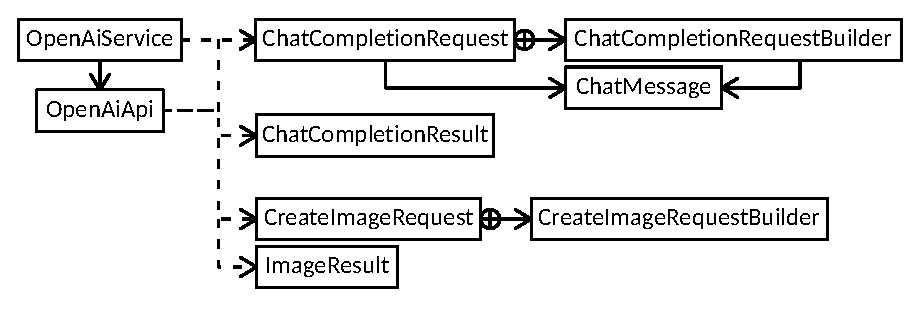
\includegraphics{chapter/chapter_3/mechanisms/openai-endpoint-mech.eps}
    \caption{Endpunkte der OpenAI Schnittstelle.}
    \label{sec3:model:subsubsec:genai-integration:fig:openai-endpoint-comps}
\end{figure}

\cref{sec3:model:subsubsec:genai-integration:fig:openai-endpoint-comps} zeigt ein partielles Klassendiagramm, welches die an der Erstellung von Anfragen an die Endpunkte der Schnittstelle beteiligten Komponenten zeigt.
Die Komponenten \textit{OpenAiService} und \textit{OpenAiApi} bieten Zugriff auf die Funktionalitäten der Schnittstelle und behandeln zudem die Konfiguration der Schnittstelle.
Weitere Komponenten sind \textit{ChatCompletionRequest} und \textit{CreateImageRequest}, die jeweils als Objekt eine Anfrage an einen Endpunkt darstellen.
Die Anfragen müssen dann noch über die Komponente \textit{OpenAiService} an die Schnittstelle gesendet werden.
Analog zu den Anfragen sind die Komponenten \textit{ChatCompletionResult} und \textit{ImageResult} Container, die die Ergebnisse der Anfragen an die jeweiligen Endpunkte speichern.
Folglich bestehen diese Komponenten wiederum aus kleinen weiteren Komponenten, die die jeweiligen Informationen speichern.
Die Komponenten \textit{ChatCompletionRequestBuilder} und \textit{CreateImageRequestBuilder} sind jeweils die Komponenten, die die Parameter der Anfrage spezifizieren.
Inbesondere ist in Bezug auf die Anfragen zur Generierung von Text die Komponente \textit{ChatMessage} von Bedeutung.
Während bei normalen Anfragen, wie z.B. der Anfrage zur Generierung von Bildern nur einfache Texteingaben benötigt werden, wird bei der Anfrage von Text eine Reihe an Textnachrichten (\textit{ChatMessage}) benötigt, die einen Dialog zwischen mehreren Parteien darstellen.
Eine Textnachricht erwartet als Eingabe eine Rolle im Dialog, sowie den Inhalt dieser Partei im Dialog.

Die genannten Komponenten stellen die Grundlage zum Erstellen einer Anfrage an die Endpunkte der Schnittstelle von OpenAI dar.
Im Folgenden ist es nun von Interesse herauszufinden, welche Informationen für das Erstellen einer effektiven und sinnvollen Anfrage an einen Endpunkt der Schnittstelle notwendig sind, und welche Komponenten am Erzeugen dieser Informationen beteiligt sind.
Speziell für die Textgenerierung bestehen die Informationen für den Dialog, der durch eine Reihe an Textnachrichten \textit{ChatMessage} dargestellt wird, zumeist aus Instruktionen (siehe z.B. \cref{sec3:model:subsubsec:explainability-through-genai}), sowie den in Textformat transformierten Informationen aus einem Graph Code (siehe \cref{sec3:model:subsubsec:gc-transformation}).

Der Prozess der Verarbeitung der Informationen eines Graph Codes wird, wie bereits durch das Sequenzdiagramm für den Anwendungsfall \hyperref[sec3:model:uc-1.3]{UC-1.3} dargestellt, von einem Benutzer durch die Auswahl eines Graph Codes initiiert.
Schlussendlich wird dann der Komponente \textit{ExplanationPanel} ein Graph Code übergeben, welche diesen Graph Code dann an die spezifischen Komponenten \textit{ImagePanel} und \textit{TextPanel} der Erklärungstypen \textit{Image} oder \textit{Text} delegiert.
Die Verarbeitung der Informationen erfolgt dann gesondert und abhängig vom Erklärungstyp durch die Komponenten \textit{TextPanel} oder \textit{ImagePanel} in der Methode \textit{setUpPrompt}.
Ein Beispiel für die Zusammenstellung der durch die Transformation generierten Informationen in der Methode \textit{setUpPrompt} kann in folgendem Beispiel eingesehen werden:

\begin{tcolorbox}[enhanced, colback=white,segmentation style={solid}, breakable]
  \textbf{System}: \enquote{You are an assistant, who is able to generate cohesive textual explanations based on a collection of words.}
  \tcbline
  \textbf{Assistant}: \enquote{The collection of words represents a dictionary. The dictionary contains so-called feature vocabulary terms. Some of the dictionary terms are connected through a relationship. These relationships will be noted as $<i_{t}> - <i_{t_{1}},...,i_{t_{n}}>$ or $<i_{t}> k <i_{t_{1}},...,i_{t_{n}}>$, where $i_{t}$ denotes the index of a feature vocabulary term. Additionally $-$ represents an undefined relationship, while $k$ represents a specific relationship.}.
  \tcbline
  \textbf{User}: \enquote{The collections of words is as follows: <\textit{Liste der Merkmale aus dem Wörterbuch eines Graph Codes}>. The relationships are as follows: <\textit{Generierte Formate der Beziehungen durch einen Graph Code}>. Generate a coherent textual explanation containing the terms of the dictionary. An example for such an explanation could be: <\textit{Beispiel zur Verdeutlichung...}>.}.
  \tcbline
  \textbf{Assistant}: \enquote{Based on the dictionary, here is a cohesive textual explanation containing the terms of the dictionary:}.
\end{tcolorbox}

Die Verarbeitung der durch die Transformation generierten Informationen und in einer Prompt zusammengetragenen Informationen wird im Folgenden durch einen allgemeinen \cref{sec3:model:subsubsec:genai-integration:alg:text-end} beschrieben, der die Sequenz der notwendigen Schritte und Aktionen hervorhebt, um eine Anfrage an den Endpunkt Text (\textit{ChatCompletionRequest}) zur Generierung von Text zu erstellen.

% <Pseudoalgorithmus>
\begin{algorithm}[htb]
\caption{Anfrage an den Endpunkt Text (\textit{ChatCompletionRequest}).}
\label{sec3:model:subsubsec:genai-integration:alg:text-end}
\begin{algorithmic}[1]
\Procedure{createRequest}{}
  \State Service initialisieren... (\textit{OpenAiService})
  \State Anfrage initialisieren... (\textit{ChatCompletionRequest})
  \State Anfrage anpassen, Parameter setzen... (\textit{ChatCompletionRequestBuilder})
  \State Anfrage an Schnittstelle senden (\textit{OpenAiService})
  \State Ergebnis erhalten und entsprechend verwerten (\textit{ChatCompletionResult}, \textit{TextPanel})
\EndProcedure
\end{algorithmic}
\end{algorithm}


Bezüglich der Erstellung einer Anfrage an den Endpunkt Bild (\textit{ImageRequest}) zum Generieren eines Bildes besteht allerdings das Problem der Tokenbegrenzung von Dall-E 2.
Im Folgenden wird ein Konzept entwickelt, um diesem Problem zu begegnen.
Dieses Konzept sieht das In-Reihe-Schalten der Endpunkte vor.
Genauer wird zuerst eine Anfrage an den Endpunkt Text zum Generieren von Text erstellt und gesendet, um darauffolgend mit dem daraus resultierenden Ergebnis die Eingabe für eine Anfrage an den Endpunkt Bild zu speisen.
Dies ist möglich, da die Anfrage an den Endpunkt Text spezifisch dazu parametrisiert werden kann, dass das Ergebnis dieser Anfrage nur eine maximale Länge an Zeichen umfassen darf/soll.
Des Weiteren können die Instruktionen der Prompt zur Generierung von Text so angepasst werden, dass dem System generativer KI vermittelt wird, dass das erzeugte Ergebnis dieser Anfrage wiederum als Eingabe für ein Bilderzeugungsprogramm verwendet werden soll (siehe \cref{sec3:model:subsubsec:explainability-through-genai}, \enquote{Create a visual explanation / description.}).
Das Erzeugen einer Anfrage an den Endpunkt Bild verhält sich analog zum Endpunkt Text.

% Beschreibung der Erweiterung...

% Hier wäre es dann vermutlich noch sinnvoll auf die Zusammenstellung der in \cref{sec3:model:subsubsec:gc-transformation} generierten Informationen zu sprechen... Dies würde dann in erster Linie ein Pseudoalgorithmus für die Erstellung einer Anfrage an den Endpunkt Text (ChatCompletionRequest) sein... Gesondert wird dann noch darüber gesprochen, wie das Problem mit der Tokenbegrenzung für den Endpunkt Bild (ImageRequest) gehandhabt werden kann -> Erst Textanfrage mit spezifischen Anfrageparametern (geringe Tokenzahl der Antwort...), dann Bildanfrage (also in Reihe geschalten) (hierfür dann eventuell eine Erweiterung des Pseudoalgorithmus oder nur eine detaillierte Beschreibung des Ablaufs) -> nur eine detaillierte Beschreibung

% Zusammenstellung der generierten Informationen aus der Transformation ansprechen...
% Dies wird in erster Linie ein Pseudoalg für die Erstellung einer Anfrage an den Endpunkt Text sein (ChatCompletionRequest)
% Gesondert sollte dann darüber gesprochen werden, wie das Problem mit der Tokenbegrenzung für den Endpunkt Bild gehandhabt werden kann...
% In Reihe schalten (Text, dann Bild) mit einer spezifischen Textanfrage und passenden Anfrageparametern (geringe Tokenanzahl)
% Nur Beschreibung des Vorgehens für eine Bildanfrage (also Erweiterung nur textuell beschreiben, kein eigener Pseudoalg).

Mit diesen neuen Informationen kann eine Erweiterung bzw. Ergänzung des Sequenzdiagramms für den Anwendungsfall \hyperref[sec3:model:uc-1.3]{UC-1.3} vorgenommen werden.
\cref{sec3:model:par:seq-use-cases:fig:seq-diag-uc-1.3-exp} zeigt die Erweiterung des Sequenzdiagramms um die neuen Abläufe der Verarbeitung von Graph Codes in den Komponenten \textit{ImagePanel} und \textit{TextPanel}.

\begin{figure}[htb]
    \centering
    \resizebox{\textwidth}{!}{
        \begin{tikzpicture}
            \begin{umlseqdiag}
                
                \umlmlobject[x=0, fill=white]{gcs}{\shortstack[c]{Graph Code \\ SelectionListener}}
                \umlmlobject[x=4, fill=white]{ep}{\shortstack[c]{Explanation \\ Panel}}
                \umlmlobject[x=8, fill=white]{imgp}{\shortstack[c]{ImagePanel}}
                \umlmlobject[x=11, fill=white]{txtp}{\shortstack[c]{TextPanel}}

                % Calls
                \begin{umlcall}[padding=0,dt=6,op={Setze Graph Code}]{gcs}{ep}
                    \begin{umlcall}[op={Setze Graph Code}]{ep}{imgp}
                        \begin{umlcallself}[op={\shortstack[c]{Verarbeite\\GraphCode}}]{imgp}
                        \end{umlcallself}
                    \end{umlcall}
                    \begin{umlcall}[dt=4,op={Setze Graph Code}]{ep}{txtp}
                        \begin{umlcallself}[op={\shortstack[c]{Verarbeite\\GraphCode}}]{txtp}
                        \end{umlcallself}
                    \end{umlcall}
                \end{umlcall}
            \end{umlseqdiag}
        \end{tikzpicture}
    }
    \caption{Erweiterung zum Sequenzdiagramm für den Anwendungsfall \hyperref[sec3:model:uc-1.3]{UC-1.3}.}
    \label{sec3:model:par:seq-use-cases:fig:seq-diag-uc-1.3-exp}
\end{figure}

Weitere Parameter zum Anpassen einer Anfrage an einen Endpunkt der Schnittstelle können durch die Benutzerschnittstellen, dargestellt in \cref{sec3:model:par:wireframe:fig:stage-2+3}, generiert werden.
Genauer würden die Spezifikationen der Anfragen an die Endpunkte der Schnittstelle durch die gewählten Einstellungen im Rahmen des Anwendungsfall \hyperref[sec3:model:uc-1.7]{UC-1.7} in den erweiterten Optionen (siehe \cref{sec3:model:par:wireframe:fig:stage-2+3} \circitem{9}) zustande kommen.

Anhand dieser Informationen kann nun auch ein Mechanismus für den Anwendungsfall \hyperref[sec3:model:uc-1.8]{UC-1.8} erstellt werden (siehe \cref{sec3:model:par:mechanism-use-cases:fig:mech-uc-1.8}).
Der Anwendungsfall \hyperref[sec3:model:uc-1.8]{UC-1.8} \enquote{Erklärung generieren} beginnt durch das Klicken des Knopfes \enquote{Generate ...}.
Im weiteren Verlauf erzeugt das System dann die notwendigen Komponenten für eine Anfrage an einen Endpunkt der Schnittstelle.
Diese Objekte werden dann durch durch die in den erweiterten Optionen gewählten Einstellungen parametrisiert und die Anfrage finalisiert.
Schlussendlich übergibt das System die Anfrage an die Komponente \textit{OpenAiService}, welche die Anfrage dann an die Schnittstelle sendet und auf diese Weise eine Erklärung generieren lässt.
Es ist wichtig anzumerken, dass diese Beschreibung für das Generieren von Erklärungen sehr generisch ist und für beide Erklärungstypen gilt.

\begin{figure}[htb]
    \centering
    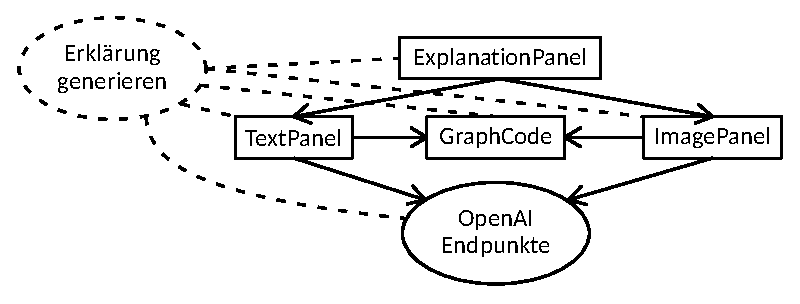
\includegraphics{chapter/chapter_3/mechanisms/mechanism-uc-1.8.eps}
    \caption{Mechanismus für den Anwendungsfall \hyperref[sec3:model:uc-1.8]{UC-1.8}.}
    \label{sec3:model:par:mechanism-use-cases:fig:mech-uc-1.8}
\end{figure}

\begin{figure}[htb]
    \centering
    \resizebox{\textwidth}{!}{
        \begin{tikzpicture}
            \begin{umlseqdiag}
                % Actors
                \umlactor[fill=white, scale=0.7]{Benutzer}

                % Objects
                \umlobject[x=0, fill=white]{Benutzer}
                \umlmlobject[x=3.3, fill=white]{tip}{\shortstack[c]{(Text/Image)Panel}}
                \umlmlobject[x=7, fill=white]{rq}{(...)Request}
                \umlmlobject[x=10, fill=white]{bld}{\shortstack[c]{(...)Request\\Builder}}
                \umlmlobject[x=13, fill=white]{oas}{OpenAiService}


                % Calls
                \begin{umlcall}[padding=0,dt=7,op={\shortstack[c]{Erklärung \\ generieren}}]{Benutzer}{tip}
                    \begin{umlcall}[padding=2.5,op={Erzeuge Anfrage},return={Anfrage}]{tip}{rq}
                    \end{umlcall}
                    \begin{umlcall}[padding=2.5,dt=4,op={Parameter der Anfrage anpassen}, return={Modifizierte Anfrage}]{tip}{bld}
                    \end{umlcall}
                    \begin{umlcall}[padding=2.5,dt=4,op={Anfrage an Endpunkt senden}, return={Ergebnis in Form von (Text/Bild)}]{tip}{oas}
                    \end{umlcall}
                    \begin{umlcallself}[dt=4,op={\shortstack[c]{Ergebnis\\verarbeiten\\/ anzeigen}}]{tip}
                    \end{umlcallself}
                \end{umlcall}
            \end{umlseqdiag}
        \end{tikzpicture}
    }
    \caption{UML-Sequenzdiagramm für den Anwendungsfall \hyperref[sec3:model:uc-1.8]{UC-1.8}.}
    \label{sec3:model:par:seq-use-cases:fig:seq-diag-uc-1.8}
\end{figure}


\cref{sec3:model:par:seq-use-cases:fig:seq-diag-uc-1.8} zeigt ein Sequenzdiagramm für den Anwendungsfall \hyperref[sec3:model:uc-1.8]{UC-1.8}.
Es zeigt, wie der Benutzer die Aktion \enquote{Erklärung generieren} durch einen Klick auf den Knopf \enquote{Generate ...} initiiert.
Die Abbildung stellt dabei eine generische Darstellung eines Ablaufs zum Generieren einer Erklärung dar und gilt für beide Komponenten \textit{ImagePanel} und \textit{TextPanel}.
Im weiteren Verlauf wird dann die notwendigen Komponenten, die für eine Anfrage benötigt werden, erzeugt und anhand von Benutzereingaben parametrisiert bzw. deren Parameter modifiziert.
Hierzu gehören im Übrigen auch die Eingabeaufforderungen / Prompt, die die bereits verarbeiteten Informationen aus einem Graph Code enthalten.
Diese angepasste Anfrage kann dann über den Endpunkt an die Schnittstelle gesendet werden.
Nach Fertigstellung der Verarbeitung seitens des Systems generativer KI, wird über die Schnittstelle ein Ergebnis, abhängig vom Erklärungstyp, zurückgeliefert.
Dieses Ergebnis kann dann schlussendlich von der Komponente \textit{ImagePanel} oder \textit{TextPanel} weiterverarbeitet oder angezeigt werden.

\FloatBarrier

\subsubsection{Diskussion}
\label{sec3:model:subsubsec:fz2:discussion}
In diesem Abschnitt wurden die offenen Herausforderungen \hyperref[sec2:sota:oi:2.1]{\textbf{OH 2.1}} und \hyperref[sec2:sota:oi:2.2]{\textbf{OH 2.2}} adressiert.
In \cref{sec3:model:subsubsec:gc-transformation} wurde die offene Herausforderung \hyperref[sec2:sota:oi:2.1]{\textbf{OH 2.1}} behandelt und Konzepte zur Transformation von Graph Codes vorgestellt, mit welchen Graph Codes in eine geeignete Form zur Eingabe in Systeme generativer KI transformiert werden sollen.
In Abschnitt \cref{sec3:model:subsubsec:genai-integration} wurde die offene Herausforderung \hyperref[sec2:sota:oi:2.2]{\textbf{OH 2.2}} behandelt und Konzepte zur Integration von Systemen generativer KI vorgestellt.

\clearpage

\subsection{Zusammenfassung}
\label{sec3:model:subsec:summary}
In diesem Kapitel wurde die Modellierung behandelt und es wurden in \cref{sec3:model:subsec:fz-explainability} Konzepte für die Erklärbarkeit von MMIR mittels generativer KI, sowie in \cref{sec3:model:subsec:fz-integration} Konzepte für die Integration von generativer KI in das GMAF entwickelt.
In \cref{sec3:model:subsubsec:summary-findings} werden die in diesem Kapitel gewonnen Erkentnisse zusammengefasst, in \cref{sec3:model:subsubsec:futher-approach} wird das weitere Vorgehen festgehalten und schlussendlich in \cref{sec3:model:subsec:summary:table:summary} eine Übersicht des aktuellen Arbeitstands in einer Tabelle dargestellt.

\subsubsection{Gewonnene Erkenntnisse}
\label{sec3:model:subsubsec:summary-findings}
In diesem Abschnitt werden die Erkenntnisse aus den Forschungszielen \enquote{FZ 1.2/TB Erklärbarkeit von MMIR mittels generativer KI} und \enquote{FZ 2.2/TB Integration generativer KI in das GMAF} zusammengefasst.

Im ersten Forschungsziel wurde angesprochen, wie Erklärbarkeit durch generative KI erreicht werden kann.
Darüber hinaus wurden in Bezug auf das GMAF eine Reihe an benutzerorientierten Anwendungsfällen identifiziert und textuell beschrieben.
Anhand dieser Anwendungsfälle wurden schrittweise Benutzerschnittstellen mit geeigneten Interaktionsmöglichkeiten konzipiert.
Des Weiteren wurden mit Hilfe von Mechanismen, die an Anwendungsfällen beteiligten Komponenten identifiziert, anhand derer wiederum Sequenz- bzw. Interaktionsdiagramme und Pseudoalgorithmen erstellt werden konnten.

Im zweiten Forschungsziel wurde die Transformation der in Graph Codes gespeicherten, sowie der mit Graph Codes assoziierten Informationen behandelt und es wurden Konzepte zur Überführung dieser Informationen in eine geeignete Form, den Prompts, in Systeme generativer KI entwickelt.
Zusätzlich wurde die Einbindung der Systeme generativer KI in das GMAF behandelt und Konzepte zur Integration dieser in das GMAF entwickelt.

Die in den \cref{sec3:model:subsec:fz-explainability,sec3:model:subsec:fz-integration} gewonnenen Erkenntnisse münden in folgendem Klassendiagramm (siehe \cref{sec3:model:subsec:summary:fig:class-diagram}), in welchem die identifizierten und für die Modellierung wichtigen Klassen, sowie die Beziehungen in denen sie zueinander stehen übersichtlich dargestellt werden.

\begin{figure}[htb]
  \centering
  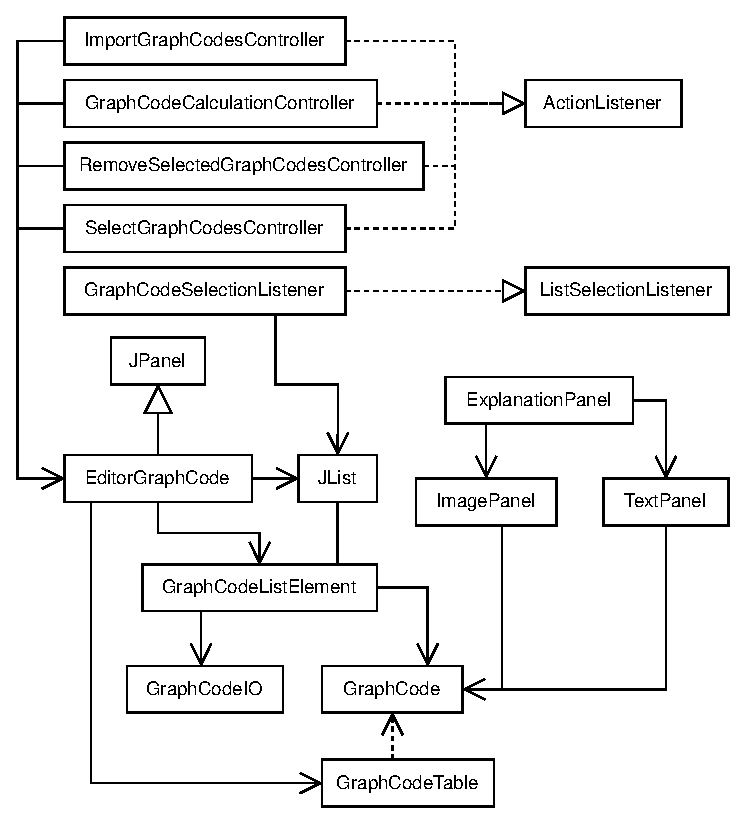
\includegraphics[width=0.8\textwidth]{chapter/chapter_3/class.eps}
  \caption{Klassendiagramm.}
  \label{sec3:model:subsec:summary:fig:class-diagram}
\end{figure}

\FloatBarrier

\subsubsection{Weiteres Vorgehen}
\label{sec3:model:subsubsec:futher-approach}
Im folgenden Kapitel werden die in diesem Kapitel entwickelten Konzepte im Rahmen einer Implementierung durch ihre entsprechenden Forschungsziele untersucht.
Genauer werden in \cref{sec4:impl} in FZ 1.3/I Benutzerschnittstellen und Funktionen implementiert und in FZ 2.3/I die Integration der Systeme generativer KI, sowie die Überführung der Informationen von und um Graph Codes zur Generierung von Erklärungen umgesetzt.

Die nachfolgende Tabelle stellt eine Erweiterung der \cref{sec2:sota:subsec:summary:table:summary} dar und gibt eine Übersicht über den aktuellen Arbeitsstand nach Abschluss dieses Kapitels.

\begingroup
\def\arraystretch{1.1}%
\begin{xltabular}{\linewidth}{
            @{}
            >{
                \hsize=0.2\linewidth
                \raggedright\arraybackslash
            }X
            >{
                \hsize=0.6\linewidth
                \raggedright\arraybackslash
            }X
            >{
                \hsize=0.2\linewidth
            }X
            @{}
        }

        % First Header

        \caption{Tabelle zur Übersicht des aktuellen Arbeitstands.}
        \label{sec3:model:subsec:summary:table:summary}
        \\

        \toprule
        \multicolumn{3}{
            >{
                    \hsize=\linewidth\centering\arraybackslash
            }X
        }
        {
            \textbf{Forschungsziele}
        } \\ \midrule
        \textbf{FZ / OH} &  \textbf{Beschreibung} & \textbf{Referenz} \\ \midrule

        \endfirsthead

        \toprule
        \multicolumn{3}{
            >{
                    \hsize=\linewidth\centering\arraybackslash
            }X
        }
        {
            \textbf{Forschungsziele}
        } \\ \midrule
        \textbf{FZ / OH} & \textbf{Beschreibung} & \textbf{Referenz} \\ \midrule

        \endhead

        % Lower Rows

        \multicolumn{3}{
            >{
                    \hsize=\linewidth\centering\arraybackslash
            }X
        }
        {
            \textbf{Erklärbarkeit von MMIR mittels generativer KI}
        }
        \\
        \midrule

        FZ 1.1/O
        &
        Recherche zur Erklärbarkeit von MMIR mittels generativer KI
        \\

        &
        Grundlegende Technologien:
        &

        \\

        &
        \tabitem GMAF
        &
        \cref{sec2:sota:subsubsec:gmaf}
        \\

        &
        \tabitem MMFG
        &
        \cref{sec2:sota:subsubsec:mmfg}
        \\

        &
        \tabitem Graph Code
        &
        \cref{sec2:sota:subsubsec:graph-codes}
        \\

        % Offene Herausforderungen aus FZ1/O

        OH 1.1
        &
        Erste offene Herausforderung
        &
        \hyperref[sec2:sota:oi:1.1]{\textbf{OH 1.1}}
        \\


        &
        Systeme generativer KI und ein Überlick über aktuelle Systeme
        &
        \cref{sec2:sota:subsubsec:genai}
        \\

        &
        Diskussion und Auswahl von Systemen
        &
        \cref{sec2:sota:subsubsec:fz1:discussion}
        \\

        OH 1.2
        &
        Zweite offene Herausforderung
        &
        \hyperref[sec2:sota:oi:2.1]{\textbf{OH 2.1}}
        \\

        \midrule

        FZ 1.2/TB
        &
        Modellierung der Erklärbarkeit von MMIR mittels generativer KI
        &

        \\

        &
        Erklärbarkeit durch generative KI
        &
        \cref{sec3:model:subsubsec:explainability-through-genai}
        \\

        &
        $\rightarrow$ Behandlung der ersten offenen Herausforderung \hyperref[sec2:sota:oi:1.1]{\textbf{OH 1.1}}
        &
        \\

        &
        Anwendungsfälle:
        &
        \cref{sec3:model:subsubsec:use-cases}
        \\

        &
        \tabitem Textuelle Beschreibungen
        &
        %\cref{sec3:model:par:textual-desc-use-cases}
        \\

        &
        \tabitem Wireframes
        &
        %\cref{sec3:model:par:wireframe}
        \\

        &
        \tabitem Mechanismen
        &
        %\cref{sec3:model:par:mechanism-use-cases}
        \\

        &
        \tabitem Sequenzdiagramme
        &
        %\cref{sec3:model:par:seq-use-cases}
        \\

        &
        $\rightarrow$ Behandlung der zweiten offenen Herausforderung \hyperref[sec2:sota:oi:1.2]{\textbf{OH 1.2}}
        &
        \\

        \midrule

        FZ 1.3/I
        &
        Implementierung der Erklärbarkeit von MMIR mittels generativer KI
        &

        \\

        \midrule

        FZ 1.4/E
        &
        Evaluierung der Erklärbarkeit von MMIR mittels generativer KI
        &

        \\

        \midrule

        \multicolumn{3}{
            >{
                    \hsize=\linewidth\centering\arraybackslash
            }X
        }
        {
            \textbf{Integration generativer KI in das GMAF}
        }
        \\
        \midrule

        FZ 2.1/O
        &
        Recherche zur Integration generativer KI in das GMAF
        &

        \\


        &
        Aufzeigen der Integrationsmöglichkeiten von:
        &

        \\

        &
        \tabitem Graph Codes
        &
        \cref{sec2:sota:subsubsec:gc-capabilities-integration}
        \\

        &
        Erste offene Herausforderung
        &
        \hyperref[sec2:sota:oi:2.1]{\textbf{OH 2.1}}
        \\

        &
        \tabitem Systemen generativer KI
        &
        \cref{sec2:sota:subsubsec:genai-capabilities-integration}
        \\

        &
        Zweite offene Herausforderung
        &
        \hyperref[sec2:sota:oi:2.2]{\textbf{OH 2.2}}
        \\

        \midrule

        FZ 2.2/TB
        &
        Modellierung der Integration generativer KI in das GMAF
        &

        \\

        &
        Transformation von Graph Codes
        &
        \cref{sec3:model:subsubsec:gc-transformation}
        \\

        &
        \tabitem Transformation des Vokabulars
        &
        \\

        &
        \tabitem Transformation der Matrix
        &
        \\

        &
        \tabitem Anwendung von Graph Code Metriken
        &
        \\

        &
        $\rightarrow$ Behandlung der ersten offenen Herausforderung \hyperref[sec2:sota:oi:2.1]{\textbf{OH 2.1}}
        &
        \\

        &
        Einbindung generativer KI in das GMAF
        &
        \cref{sec3:model:subsubsec:genai-integration}
        \\

        &
        $\rightarrow$ Behandlung der zweiten offenen Herausforderung \hyperref[sec2:sota:oi:2.2]{\textbf{OH 2.2}}
        &
        \\

        \midrule

        FZ 2.3/I
        &
        Implementierung der Integration generativer KI in das GMAF
        &

        \\

        \midrule

        FZ 2.4/E
        &
        Evaluierung der Integration generativer KI in das GMAF
        &

        \\

        \bottomrule
\end{xltabular}
\endgroup



\section{Implementierung}
\label{sec4:impl}
Dieses Kapitel widmet sich der Implementierung und es werden, entsprechend der Methodik von Nunamaker \cite{nunamaker}, alle Forschungsziele der Implementierungsphase behandelt.
Ziel der Implementierung ist die Untersuchung und Validierung der in \cref{sec3:model} beschriebenen Modellierung, und die Vorbereitung einer detaillierten Evaluierung in der Experimentphase, sowie Untersuchungen weiterer Beobachtungen, die während der Implementierung gemacht wurden.
Die Struktur dieses Kapitels folgt der logischen Abfolge der Forschungsziele der Implementierungsphase.
Doch zuvor werden in \cref{sec4:impl:subsec:basics} die Grundlagen bzw. Vorbereitungen für die Implementierung getroffen.
Dies umfasst die Beschreibung der geplanten Struktur und Architektur der Implementierung, sowie weitere technische Voraussetzungen und die in dieser prototypischen Implementierung genutzten Bibliotheken bzw. Abhängigkeiten.
In \cref{sec4:impl:subsec:fz-explainability} werden ausgewählte Implementierungsdetails der Erklärbarkeit von MMIR mittels generativer KI vorgestellt.
Dies umfasst besonders die Benutzeroberfläche, ihre Benutzerelemente und die Interaktion mit diesen.
Analog dazu werden in \cref{sec4:impl:subsec:fz-integration} ausgewählte Implementierungsdetails der Integration generativer KI in das GMAF vorgestellt.
Dies umfasst die Transformation von Graph Codes und die Integration der Schnittstelle von OpenAI und ihre Endpunkte.

{
    \def\arraystretch{1.1}%
    \begin{xltabular}{\linewidth}{
            @{}
            >{
                \hsize=0.25\linewidth
                \raggedright\arraybackslash
            }X
            >{
                \hsize=0.55\linewidth
                \raggedright\arraybackslash
            }X
            >{
                \hsize=0.2\linewidth
                \centering\arraybackslash
            }X
            @{}
    }

    % First Header

    \caption{Struktur des Kapitels 4 \enquote{Implementierung}.}
    \label{sec4:impl:table:structure} \\

    \toprule

    \textbf{FZ} & \textbf{Kurze Beschreibung} & \textbf{Abschnitt} \\

    \midrule

    \endfirsthead

    % Normal Head

    \toprule

    \textbf{FZ} & \textbf{Kurze Beschreibung} & \textbf{Abschnitt} \\

    \midrule

    \endhead

    % Lower Rows

    Grundlagen der Implementierung & Technische Grundlagen & \cref{sec4:impl:subsec:basics} \\
    FZ 1.3/I & Implementierung: Benutzerschnittstelle & \cref{sec4:impl:subsec:fz-explainability} \\
    FZ 2.3/I & Implementierung: Transformation von Graph Codes \& Integration gen. KI & \cref{sec4:impl:subsec:fz-integration} \\
    Zusammenfassung & Ergebnisse / Erkenntnisse & \cref{sec4:impl:subsec:summary} \\

    \bottomrule

    \end{xltabular}
}


\subsection{Grundlagen der Implementierung}
\label{sec4:impl:subsec:basics}
In diesem Abschnitt werden die Grundlagen für die in diesem Kapitel beschriebene prototypische Proof-of-Concept Implementierung festgehalten.
Dies umfasst die allgemeine Architektur, ihr zugrunde liegendes Prinzip, ihr hierarchischer Aufbau, sowie die Abhängigkeiten zu Drittanbieter-Bibliotheken.

\paragraph{Architekturmuster}
Die Implementierung der Software folgt dem Muster des \textit{Model-View-Controller}-Prinzips und teilt die Architektur der Software in drei seperate Bereiche: \textit{Model} für die Datenstrukturen, \textit{View} für das Frontend bzw. die Benutzerschnittstellen und \textit{Controller} zum Handhaben von Ereignissen und Interaktionen zwischen den Bereichen \textit{Model} und \textit{View}.
Ziel dieser Architektur ist durch das gezielte Trennen dieser Bereiche die Eigenschaften wie Wiederverwendbarkeit, Wartbarkeit und Robustheit der Software zu erhöhen und zu stärken.

Das erste Forschungsziel \hyperref[sec4:impl:subsec:fz-explainability]{FZ 1.3/I} widmet sich der Benutzerschnittstelle, ihren Elementen und der Interaktion mit diesen und deckt somit die Bereiche \textit{View, Controller} ab.
Das zweite Forschungsziel \hyperref[sec4:impl:subsec:fz-integration]{FZ 2.3/I} widmet sich der Transformation von Graph Codes und der Integration der Schnittstelle und ihren Endpunkten und deckt somit den Bereich \textit{Model} ab.

\cref{sec4:impl:subsec:basiscs:fig:hierarchy} zeigt die Hierarchie des Quellcodes, der in diesem Kapitel beschriebenen prototypischen Proof-of-Concept Implementierung.

\def\Size{4pt}
\tikzset{
      folder/.pic={
        \filldraw[draw=folderborder,top color=folderbg!50,bottom color=folderbg]
          (-1.05*\Size,0.2\Size+5pt) rectangle ++(.75*\Size,-0.2\Size-5pt);  
        \filldraw[draw=folderborder,top color=folderbg!50,bottom color=folderbg]
          (-1.15*\Size,-\Size) rectangle (1.15*\Size,\Size);
      }
    }

\begin{figure}[htb]
\begin{forest}
      for tree={
        font=\ttfamily,
        grow'=0,
        child anchor=west,
        parent anchor=south,
        anchor=west,
        calign=first,
        inner xsep=7pt,
        edge path={
          \noexpand\path [draw, \forestoption{edge}]
          (!u.south west) +(7.5pt,0) |- (.child anchor) pic {folder} \forestoption{edge label};
        },
        % style for your file node 
        file/.style={edge path={\noexpand\path [draw, \forestoption{edge}]
          (!u.south west) +(7.5pt,0) |- (.child anchor) \forestoption{edge label};},
          inner xsep=2pt,font=\small\ttfamily
                     },
        before typesetting nodes={
          if n=1
            {insert before={[,phantom]}}
            {}
        },
        fit=band,
        before computing xy={l=15pt},
      }  
    [de
        [ja
            [controller]
            [model]
            [view]
        ]
        [swa]
    ]
\end{forest}
\caption{Hierarchie des Quellcodes.}
\label{sec4:impl:subsec:basiscs:fig:hierarchy}
\end{figure}

\paragraph{Abhängigkeiten (Maven)}
Für die prototypische Proof-of-Concept Implementierung der in \cref{sec3:model} vorgestellten konzeptuellen Modellierung wird die Programmiersprache Java \cite{java} ausgewählt.
Der in diesem Kapitel vorgestellte Quellcode ist auf GitHub verfügbar.
Die Implementierung in Java baut hierbei auf Maven \cite{maven}, einem Build-Tool der Apache Software Foundation für die Projektverwaltung und Management von Abhängigkeiten, auf.
Im Folgenden werden die in diesem Projekt verwendet Abhängigkeiten aufgezählt und ihre Verwendungszwecke genannt.

\begin{tcolorbox}
    [enhanced,
     colback=white,
     colbacktitle=white,
     coltitle=black,
     title=OpenAI-Java,
     toptitle=1.5mm,
     bottomtitle=1.5mm,
     center title,
     breakable,
     segmentation style={solid}
]
\begin{lstlisting}[
    firstnumber=1,
    language=XML,
    basicstyle=\ttfamily\footnotesize,
    breaklines=true
]
<!-- https://mvnrepository.com/artifact/com.theokanning.openai-gpt3-java/service -->
<dependency>
  <groupId>com.theokanning.openai-gpt3-java</groupId>
  <artifactId>service</artifactId>
  <version>0.13.0</version>
</dependency>
\end{lstlisting}
\tcbline
\textbf{Verwendungszweck}: Diese Abhängigkeit stellt die Schnittstelle von OpenAI und ihre Endpunkte in Java bereit.
\end{tcolorbox}

\begin{tcolorbox}
    [enhanced,
     colback=white,
     colbacktitle=white,
     coltitle=black,
     title=JTokkit,
     toptitle=1.5mm,
     bottomtitle=1.5mm,
     center title,
     breakable,
     segmentation style={solid}
]
\begin{lstlisting}[
    firstnumber=1,
    language=XML,
    basicstyle=\ttfamily\footnotesize,
    breaklines=true
]
<!-- https://mvnrepository.com/artifact/com.knuddels/jtokkit -->
<dependency>
  <groupId>com.knuddels</groupId>
  <artifactId>jtokkit</artifactId>
  <version>0.6.1</version>
</dependency>
\end{lstlisting}
\tcbline
\textbf{Verwendungszweck}: Diese Abhängigkeit bietet Funktionen zum Verarbeiten der von OpenAI genutzten Zeichenaufteilung in Tokens.
\end{tcolorbox}

\begin{tcolorbox}
    [enhanced,
     colback=white,
     colbacktitle=white,
     coltitle=black,
     title=Abhängigkeiten für die Benutzeroberfläche,
     toptitle=1.5mm,
     bottomtitle=1.5mm,
     center title,
     breakable,
     segmentation style={solid}
]
\begin{lstlisting}[
    firstnumber=1,
    language=XML,
    basicstyle=\ttfamily\footnotesize,
    breaklines=true
]
<!-- https://mvnrepository.com/artifact/org.swinglabs/jxlayer -->
<dependency>
  <groupId>org.swinglabs</groupId>
  <artifactId>jxlayer</artifactId>
  <version>3.0.4</version>
</dependency>

<!-- https://mvnrepository.com/artifact/org.swinglabs.swingx/swingx-all -->
<dependency>
  <groupId>org.swinglabs.swingx</groupId>
  <artifactId>swingx-all</artifactId>
  <version>1.6.5</version>
</dependency>

<!-- https://mvnrepository.com/artifact/com.miglayout/miglayout -->
<dependency>
  <groupId>com.miglayout</groupId>
  <artifactId>miglayout</artifactId>
  <version>3.7.4</version>
</dependency>

<!-- https://mvnrepository.com/artifact/com.fifesoft/rsyntaxtextarea -->
<dependency>
  <groupId>com.fifesoft</groupId>
  <artifactId>rsyntaxtextarea</artifactId>
  <version>3.3.1</version>
</dependency>
\end{lstlisting}
\end{tcolorbox}

\begin{tcolorbox}
    [enhanced,
     colback=white,
     colbacktitle=white,
     coltitle=black,
     title=Google Guava,
     toptitle=1.5mm,
     bottomtitle=1.5mm,
     center title,
     breakable,
     segmentation style={solid}
]
\begin{lstlisting}[
    firstnumber=1,
    language=XML,
    basicstyle=\ttfamily\footnotesize,
    breaklines=true
]
<!-- https://mvnrepository.com/artifact/com.google.guava/guava -->
<dependency>
  <groupId>com.google.guava</groupId>
  <artifactId>guava</artifactId>
  <version>32.1.2-jre</version>
</dependency>
\end{lstlisting}
\tcbline
\textbf{Verwendungszweck}: Diese Abhängigkeit bietet Funktionen zur Datenverarbeitung.
\end{tcolorbox}


\clearpage

\subsection[FZ 1.3/I Erklärbarkeit von MMIR mittels generativer KI]{\texorpdfstring{FZ 1.2/TB Erklärbarkeit von MMIR mittels \\ generativer KI}{FZ 1.3/I Erklärbarkeit von MMIR mittels generativer KI}}
\label{sec4:impl:subsec:fz-explainability}

In diesem Abschnitt wird die prototypische Proof-of-Concept Implementierung der \enquote{Erklärbarkeit von MMIR mittels generativer KI} beschrieben und behandelt.
Die in \cref{sec3:model} identifizierten Anwendungsfälle beschreiben die Interaktionen eines Benutzers mit dem System.
Um eine geschickte Interaktion mit dem System zu ermöglichen, wird eine Benutzungsschnittstelle mit adäquaten Interaktionsmöglichkeiten benötigt.
Die Beschreibung der Implementierung solch einer Benutzungsschnittstelle wird im Folgenden in \cref{sec4:impl:subsubsec:ui} vorgenommen.
Diese Beschreibung umfasst die Elemente der Benutzeroberfläche, sowie die Interaktion zwischen diesen.

\subsubsection{Benutzungsschnittstelle}
\label{sec4:impl:subsubsec:ui}
In diesem Abschnitt wird die Implementierung der Benutzeroberfläche beschrieben.
Für eine prototypische Proof-of-Concept Implementierung der Benutzeroberfläche wird Java's \textit{Swing} verwendet.
\textit{Swing} ist ein Werkzeug für das Erstellen von grafischen Benutzungsschnittstellen bzw. oberflächen und ist ein grundlegender Bestandteil der Laufzeitumgebung von Java.
Das Benutzen von \textit{Swing} hat somit den Vorteil, dass keine zusätzliche Installation notwendig ist und \textit{Swing} somit problemlos auf beliebigen Rechnern, auf welchen Java installiert ist, ausgeführt werden kann.
\begin{figure}[!ht]
  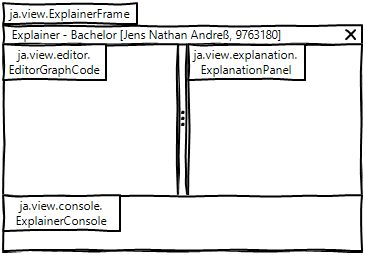
\includegraphics[width=8cm]{chapter/chapter_4/wireframe-impl-overview}
  \caption{Allgemeine Übersicht über das Mockup der Benutzungsschnittstelle.}
  \label{sec4:impl:subsubsec:ui:fig:wireframe-overview}
\end{figure}

\cref{sec4:impl:subsubsec:ui:fig:wireframe-overview} zeigt eine allgemeine Übersicht über das bereits in \cref{sec3:model:par:wireframe:fig:stage-1} vorgestellte Mockup der Benutzungsschnittstelle, erweitert um Zuweisungen der Komponenten mitsamt implementierungsspezifischen Paketnamen.
Die Elemente der in \cref{sec4:impl:subsubsec:ui:fig:wireframe-overview} gezeigten Benutzungsschnittstelle werden in \cref{sec4:impl:par:ui-elements} genauer beschrieben.
Aufbauend auf diesen Elementen wird dann in \cref{sec4:impl:par:ui-interaction} die Interaktion zwischen diesen Elementen beschrieben.
Auf diese Weise entspricht der Ablauf dieses Abschnitts dem Ablauf der Modellierung der Benutzungsschnittstelle.

\paragraph{Elemente der Benutzeroberfläche}
\label{sec4:impl:par:ui-elements}

Das Fundament der Benutzungsschnittstelle ist das \textit{ExplainerFrame}, welches durch die Klasse \textit{ja.view.ExplainerFrame} umgesetzt wird.
\cref{sec4:impl:par:ui-elements:lst:explainer-frame} zeigt die wichtigsten Aspekte der Implementierung dieser Klasse.

\lstinputlisting[style=java-code, caption={ExplainerFrame-Klasse}, label={sec4:impl:par:ui-elements:lst:explainer-frame}]{chapter/chapter_4/java/ExplainerFrame.java}

Nach der Modellierung enthält dieses Fundament drei Grundbereiche mit folgender Nummerierung (siehe \cref{sec3:model:par:wireframe:fig:stage-1}): \circitem{1} EditorGraphCode, \circitem{2} ExplainerPanel und \circitem{3} ExplainerConsole.
Diese Grundbereiche werden in \cref{sec4:impl:par:ui-elements:lst:explainer-frame} durch die privaten Variablen \textit{editorGraphCode}, \textit{explanationPanel} und \textit{explainerConsole} dargestellt.
Beim Erzeugen der Klasse \textit{ExplainerFrame} wird zuerst durch die Methode \textit{initFrame()} das Frame initialisiert und konfiguriert.
Dies umfasst die Dimension des Frames, die Position, sowie den Titel.
Darauffolgend werden dann durch die Methode \textit{initComponents()} die Komponenten, welches auch die Grundbereiche umfassen, initialisiert, konfiguriert und dem Frame hinzugefügt.
Dies umfasst besonders die notwendigen Schritte zum Hinzufügen und Layouten (z.Dt. Auslegen) der Grundbereiche im \textit{ExplainerFrame}.
Im weiteren Verlauf wird zuerst der Grundbereich \textit{EditorGraphCode}, welcher die linke Arbeitsfläche darstellt, dann der Grundbereich \textit{ExplanationPanel}, welcher die rechte Arbeitsfläche darstellt und schlussendlich der Grundbereich \textit{ExplainerConsole}, welcher die Konsole darstellt, behandelt.
Jeder dieser Grundbereiche wird mitsamt seiner enthaltenen Komponenten ausführlich behandelt, bevor mit dem nächsten Grundbereich fortgefahren wird.

\begin{figure}[!ht]
  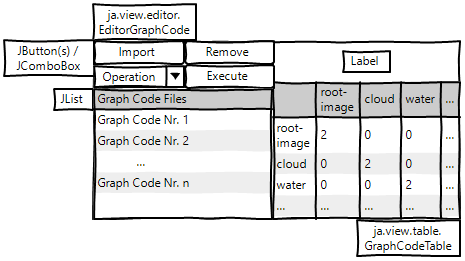
\includegraphics[width=10cm]{chapter/chapter_4/wireframe-impl-left}
  \caption{Grundbereich \textit{EditorGraphCode}.}
  \label{sec4:impl:subsubsec:ui:fig:wireframe-editor-graph-code}
\end{figure}

\cref{sec4:impl:subsubsec:ui:fig:wireframe-editor-graph-code} zeigt den Grundbereich \textit{EditorGraphCode}, umgesetzt durch die Klasse \textit{ja.view.editor.EditorGraphCode}, in welchem Benutzer durch geeignete Interaktionsmöglichkeiten die Bearbeitung von Graph Code Dateien durchführen können.
\cref{sec4:impl:par:ui-elements:lst:editor-graph-code-p1,sec4:impl:par:ui-elements:lst:editor-graph-code-p2,sec4:impl:par:ui-elements:lst:editor-graph-code-p3,sec4:impl:par:ui-elements:lst:editor-graph-code-p4} zeigen im Folgenden die wichtigsten Aspekte der Implementierung dieser Klasse.

\lstinputlisting[style=java-code, caption={EditorGraphCode-Klasse}, label={sec4:impl:par:ui-elements:lst:editor-graph-code-p1}]{chapter/chapter_4/java/egc/EditorGraphCode-P1.java}

Der Modellierung nach ist diese Arbeitsfläche in zwei nebeneinanderliegende Arbeitsflächen aufgeteilt, die in \cref{sec4:impl:par:ui-elements:lst:editor-graph-code-p1} durch die Variablen \textit{leftPart} und \textit{rightPart} dargestellt werden.
Auch diese Arbeitsflächen bestehen wiederum aus mehreren Komponenten.
Die linke Arbeitsfläche umfasst eine Schnittstelle zum Auswählen und Ausführen von Aktionen (siehe \cref{sec3:model:par:wireframe:fig:stage-2+3} \circitem{4}), dargestellt durch die Variable \textit{operationsPanel} und eine Liste an Graph Code Dateien (siehe \cref{sec3:model:par:wireframe:fig:stage-2+3} \circitem{5}), dargestellt durch die Variable \textit{graphCodeList}.
Die rechte Arbeitsfläche hingegen umfasst im Wesentlichen eine Tabelle zur Visualisierung eines ausgewählten Graph Codes (siehe \cref{sec3:model:par:wireframe:fig:stage-2+3} \circitem{6}), dargestellt durch die Variable \textit{graphCodeTable}, sowie ein Label zum Darstellen des Namens der entsprechenden Graph Code Datei über dieser Tabelle, dargestellt durch die Variable \textit{graphCodeName}.

Im Folgenden wird in \cref{sec4:impl:par:ui-elements:lst:editor-graph-code-p2}, dem zweiten Teil der EditorGraphCode-Klasse, die Schnittstelle \circitem{4} zum Auswählen und Ausführen von Aktionen genauer spezifiziert und im weiteren Verlauf erklärt.

\lstinputlisting[style=java-code, caption={EditorGraphCode-Klasse (Zweiter Teil)}, label={sec4:impl:par:ui-elements:lst:editor-graph-code-p2}, firstnumber=29]{chapter/chapter_4/java/egc/EditorGraphCode-P2.java}

Die Schnittstelle zum Auswählen und Ausführen von Aktionen, dargestellt durch \textit{operationsPanel}, besitzt vier Elemente.
Diese Elemente sind JButtons bzw. Knöpfe und eine JComboBox bzw. ein Button mit einer aus- und einklappbaren Auswahlliste und werden im Folgenden aufgezählt:
\begin{itemize}
  \item Knopf \enquote{Import Graph Code(s)}.
  Dieser Knopf ist mit dem Anwendungsfall \hyperref[sec3:model:uc-1.1]{UC-1.1} \enquote{Graph Code(s) importieren} verbunden und wird im Quellcode als Variable \textit{openGraphCodeChooserButton} eingeführt.
  Weiterhin wird die Interaktion durch ein Steuerelement \textit{ImportGraphCodesController}, welches in einem Mechanismus (siehe \cref{sec3:model:par:mechanism-use-cases:fig:mech-uc-1.1}) identifiziert werden konnte, gesteuert.
  Das an diesem Anwendungsfall beteiligte Steuerelement \textit{ImportGraphCodesController} wird in \cref{sec4:impl:par:ui-interaction:lst:import-gcs} genauer behandelt.
  \item Knopf \enquote{Remove selected Graph Code(s)}.
  Dieser Knopf ist mit dem Anwendungsfall \hyperref[sec3:model:uc-1.2]{UC-1.2} \enquote{Graph Code(s) entfernen} verbunden und wird im Quellcode als Variable \textit{removeSelectedButton} eingeführt.
  Weiterhin wird die Interaktion durch ein Steuerelement \textit{RemoveSelectedGraphCodesController}, welches in einem Mechanismus (siehe \cref{sec3:model:par:mechanism-use-cases:fig:mech-uc-1.2}) identifiziert werden konnte, gesteuert.
  Das an diesem Anwendungsfall beteiligte Steuerelement \textit{RemoveSelectedGraphCodesController} wird in \cref{sec4:impl:par:ui-elements:lst:remove-gcs} genauer behandelt.
  \item Aus- und einklappbare Auswahlliste.
  Diese Auswahlliste ist mit dem Anwendungsfall \hyperref[sec3:model:uc-1.4]{UC-1.4} \enquote{Operation auswählen} verbunden und wird im Quellcode als Variable \textit{calculationComboBox} eingeführt.
  Die Interaktion mit diesem Element wird durch das Steuerelement \textit{GraphCodeCalculationController}, welches in einem Mechanismus (siehe \cref{sec3:model:par:mechanism-use-cases:fig:mech-uc-1.5}) identifiziert werden konnte, gesteuert.
  Das an diesem Anwendungsfall beteiligte Steuerelement \textit{GraphCodeCalculationController} wird in \cref{sec4:impl:par:ui-elements:lst:calculate-gcs-p1,sec4:impl:par:ui-elements:lst:calculate-gcs-p2,sec4:impl:par:ui-elements:lst:calculate-gcs-p3,sec4:impl:par:ui-elements:lst:calculate-gcs-p4,sec4:impl:par:ui-elements:lst:calculate-gcs-p5} genauer behandelt.
  \item Knopf \enquote{Execute}.
  Dieser Knopf ist mit dem Anwendungsfall \hyperref[sec3:model:uc-1.5]{UC-1.5} verbunden und wird im Quellcode als Variable \textit{calculationOperationButton} eingeführt.
  Weiterhin wird die Interaktion ebenfalls durch das Steuerelement \textit{GraphCodeCalculationController} gesteuert.
\end{itemize}
Schlussendlich ist in \cref{sec4:impl:par:ui-elements:lst:editor-graph-code-p2} zu sehen, wie die Elemente der Schnittstelle hinzugefügt werden.
Die aus der Implementierung resultierende Schnittstelle zum Auswählen und Ausführen von Aktionen kann in \cref{sec4:impl:par:ui-elements:fig:wireframe-ui-4} eingesehen werden.

\begin{figure}[!ht]
  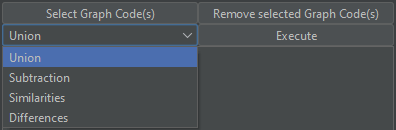
\includegraphics[width=9cm]{chapter/chapter_4/wireframe-impl-ui-4}
  \caption{Aus der Implementierung resultierende Schnittstelle zum Auswählen und Ausführen von Aktionen.}
  \label{sec4:impl:par:ui-elements:fig:wireframe-ui-4}
\end{figure}

Im Folgenden wird in \cref{sec4:impl:par:ui-elements:lst:editor-graph-code-p3}, dem dritten Teil der EditorGraphCode-Klasse, die Schnittstelle \circitem{5} bzw. Liste von Graph Codes genauer spezifiziert und im weiteren Verlauf erklärt.

\lstinputlisting[style=java-code, caption={EditorGraphCode-Klasse (Dritter Teil)}, label={sec4:impl:par:ui-elements:lst:editor-graph-code-p3}, firstnumber=52]{chapter/chapter_4/java/egc/EditorGraphCode-P3.java}

Zuerst werden Eigenschaften der Liste konfiguriert.
Eine dieser Eigenschaften ist z.B. der Auswahlmodus \textit{MULTIPLE\_INTERVAL\_SELECTION}, um eine mehrfache Auswahl in der Liste zu ermöglichen.

Die Liste ist mit dem Anwendungsfall \hyperref[sec3:model:uc-1.3]{UC-1.3} \enquote{Graph Code(s) auswählen} verbunden.
In Bezug auf den Anwendungsfall wird die Interaktion mit der Liste durch das Steuerelement \textit{GraphCodeSelectionListener} gesteuert, welches in einem Mechanismus (siehe \cref{sec3:model:par:mechanism-use-cases:fig:mech-uc-1.3}) identifiziert werden konnte.
Das Steuerelement \textit{GraphCodeSelectionListener} wird in \cref{sec4:impl:par:ui-elements:lst:select-gcs} genauer behandelt.
Zusätzlich besitzt die Liste weitere Steuerelemente, wie \textit{GraphCodeListMouseAdapter} und \textit{ListItemTransferHandler}, die ebenfalls in \cref{sec4:impl:par:ui-interaction} genauer behandelt werden.
Des Weiteren konnte in diesem Mechanismus, wie bereits auch schon in den vorherigen Mechanismen, die Komponente \textit{GraphCodeListElement} identifiziert werden.
Diese Komponente ist in Bezug auf die Liste von besonderer Bedeutung, da diese ein Element bzw. Eintrag in der Liste darstellt.
Der Quellcode für diese Komponente kann in \cref{sec4:impl:par:ui-elements:lst:gcle} eingesehen werden.

\clearpage

\lstinputlisting[style=java-code, caption={GraphCodeListElement-Klasse}, label={sec4:impl:par:ui-elements:lst:gcle}, firstnumber=1]{chapter/chapter_4/java/gcle/GraphCodeListElement.java}

\cref{sec4:impl:par:ui-elements:fig:wireframe-ui-5} zeigt ein Beispiel für die aus der Implementierung resultierende Liste mitsamt beispielhaften Einträgen für Graph Codes.

\begin{figure}[!ht]
  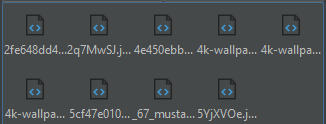
\includegraphics[width=9cm]{chapter/chapter_4/wireframe-impl-ui-5}
  \caption{Aus der Implementierung resultierende Liste mit beispielhaften Einträgen für Graph Codes.}
  \label{sec4:impl:par:ui-elements:fig:wireframe-ui-5}
\end{figure}

Schlussendlich wird in \cref{sec4:impl:par:ui-elements:lst:gct} die letzte Schnittstelle \circitem{6} \textit{GraphCodeTable} des Grundbereichs \textit{EditorGraphCode} behandelt und im weiteren Verlauf erklärt.

\lstinputlisting[style=java-code, caption={GraphCodeTable-Klasse}, label={sec4:impl:par:ui-elements:lst:gct}, firstnumber=1]{chapter/chapter_4/java/gct/GraphCodeTable.java}

Die Schnittstelle \textit{GraphCodeTable} besitzt zwei Elemente: Eine Tabelle zur Darstellung eines ausgewählten Graph Codes, umgesetzt durch ein \textit{JTable} und ein Platzhalter, zum Signalisieren, dass zu diesem Zeitpunkt noch kein Graph Code ausgewählt ist / wurde.
Die Tabelle wird in einem \textit{JScrollPane} eingebettet, um auch größere Tabellen darstellen zu können.
Des Weiteren ist ein wichtiger Teil dieser Klasse ein Datenmodell für die Tabelle, dargestellt durch die Komponente \textit{GraphCodeTableModel}.
Dieses Datenmodell wird der Tabelle zugewiesen und hat zur Aufgabe, die Informationen in einem Graph Code auf die Zeilen und Spalten der Tabelle abzubilden, sodass diese in Tabellenform dargestellt werden können.
Die wichtigste Methode der Klasse \textit{GraphCodeTable} ist \textit{setGraphCode}.
Diese Methode nimmt als Parameter einen ausgewählten Graph Code.
Anhand dieses Graph Codes werden Veränderungen an der Schnittstelle, sowie dem Datenmodell vorgenommen.
Sofern kein Graph Code ausgewählt ist, wird ein Platzhalter angezeigt.
Andernfalls wird dem Datenmodell der Graph Code zur Verarbeitung zugewiesen.

\cref{sec4:impl:par:ui-elements:fig:wireframe-ui-6} zeigt ein Beispiel für die aus der Implementierung resultierende Tabelle zur Darstellung eines ausgewählten Graph Codes.

\begin{figure}[!ht]
  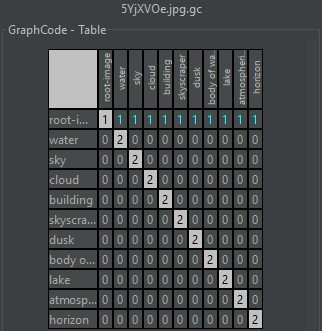
\includegraphics[width=8cm, keepaspectratio]{chapter/chapter_4/wireframe-impl-ui-6}
  \caption{Aus der Implementierung resultierende Tabelle zur Darstellung eines ausgewählten Graph Codes.}
  \label{sec4:impl:par:ui-elements:fig:wireframe-ui-6}
\end{figure}

Im Folgenden wird in \cref{sec4:impl:par:ui-elements:lst:editor-graph-code-p4}, der vierte und letzte Teil der EditorGraphCode-Klasse, genauer spezifiziert und im weiteren Verlauf erklärt.

\lstinputlisting[style=java-code, caption={EditorGraphCode-Klasse (Letzter Teil)}, label={sec4:impl:par:ui-elements:lst:editor-graph-code-p4}, firstnumber=58]{chapter/chapter_4/java/egc/EditorGraphCode-P4.java}

\cref{sec4:impl:par:ui-elements:lst:editor-graph-code-p4} zeigt das abschließende Zusammenfügen der Schnittstellen \circitem{4}, \circitem{5} und \circitem{6}.
Zusammengefügt ergeben diese Schnittstellen den Grundbereich \textit{EditorGraphCode}.
Damit ist der Grundbereich \circitem{1}, \textit{EditorGraphCode}, abgeschlossen.
\cref{sec4:impl:par:ui-elements:fig:wireframe-ui-left-complete} zeigt abschließend die vollständige Benutzeroberfläche des aus der Implementierung resultierenden Grundbereichs \textit{EditorGraphCode} mitsamt Beispielen.

\begin{figure}[!ht]
  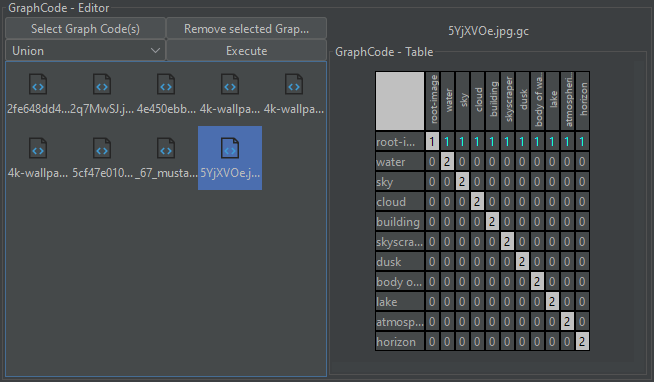
\includegraphics[width=\textwidth]{chapter/chapter_4/wireframe-impl-ui-left-complete}
  \caption{Vollständige Oberfläche des aus der Implementierung resultierenden Grundbereichs \textit{EditorGraphCode}.}
  \label{sec4:impl:par:ui-elements:fig:wireframe-ui-left-complete}
\end{figure}

Im weiteren Verlauf dieses Abschnitts wird in \cref{sec4:impl:par:ui-elements:lst:explanation-panel} der Grundbereich \circitem{2}, \textit{ExplanationPanel}, behandelt und die darin enthaltenen Schnittstellen detailliert erläutert.

\clearpage

\begin{figure}[!ht]
  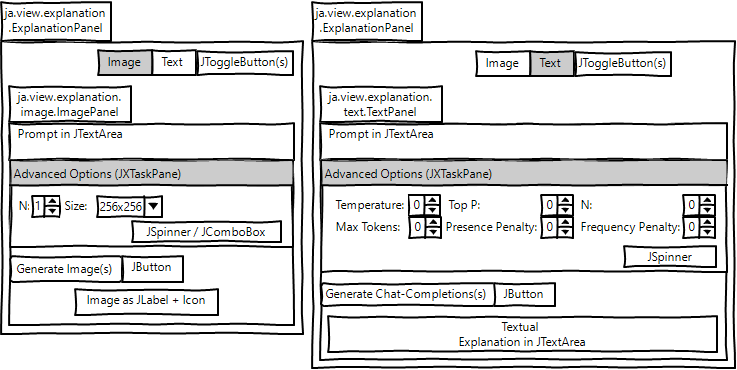
\includegraphics[width=\textwidth]{chapter/chapter_4/wireframe-impl-right}
  \caption{Grundbereich \textit{ExplanationPanel} zur Generierung von visuellen Erklärungen (links) und textuellen Erklärungen (rechts).}
  \label{sec4:impl:subsubsec:ui:fig:wireframe-explanation-panel}
\end{figure}

\cref{sec4:impl:subsubsec:ui:fig:wireframe-explanation-panel} zeigt den nächsten Grundbereich \circitem{2}, \textit{ExplanationPanel}, umgesetzt durch die Klasse \textit{ja.view.explanation.ExplanationPanel}, in welchem Benutzer durch geeignete Interaktionsmöglichkeiten die Generierung von textuellen und visuellen Erklärungen zu Graph Codes durchführen können.
Hierzu besitzt der Grundbereich \textit{ExplanationPanel} eine Fläche, in der Komponenten miteinander ausgewechselt werden können.
Genauer wird zwischen den zwei Komponenten: \textit{TextPanel} und \textit{ImagePanel}, gewechselt.

\lstinputlisting[style=java-code, caption={ExplanationPanel-Klasse}, label={sec4:impl:par:ui-elements:lst:explanation-panel}, firstnumber=1]{chapter/chapter_4/java/exp/ExplanationPanel.java}

Der Grundbereich \textit{ExplanationPanel} besitzt zwei Knöpfe (\textit{JToggleButton}) \enquote{Image} und \enquote{Text}, mit welchen zwischen den Schnittstellen \textit{ImagePanel}, zum Generieren von visuellen Erklärungen zu Graph Codes und \textit{TextPanel}, zum Generieren von textuellen Erklärungen zu Graph Codes, hin- und hergeschaltet werden kann.
Die Interaktion für diese Knöpfe wird innerhalb der Klasse durch die Methode \textit{actionPerformed} umgesetzt.
Hierfür implementiert die Klasse das Interface \textit{ActionListener} und wird den Knöpfen registriert.
Damit nur ein Knopf zeitgleich aktiviert sein kann, werden die Knöpfe einer \textit{ButtonGroup} hinzugefügt.
Die zwei Schnittstellen \textit{TextPanel} und \textit{ImagePanel} werden beide initialisiert und existieren zum selben Zeitpunkt.
Jedoch kann, in Abhängigkeit des gewählten Knopfes, immer nur eine Schnittstelle angezeigt werden.
Am Anfang ist die Schnittstelle \textit{ImagePanel} zu sehen.

Des Weiteren umfasst die Klasse zwei Methoden: \textit{setGraphCode} und \textit{actionPerformed}.
Die Methode \textit{setGraphCode} delegiert einen Graph Code an die Schnittstellen \textit{ImagePanel} und \textit{TextPanel}, wo diese dann entsprechend weiter verarbeitet werden.
Die Methode \textit{actionPerformed} wird durch das Interface \textit{ActionListener} bereitgestellt und durch die Methode \textit{addActionListener} auf die Knöpfe registriert.
Diese Methode übernimmt das Hin- und Herschalten zwischen \textit{Text}- oder \textit{ImagePanel} und entfernt \textit{TextPanel}, sofern \textit{ImagePanel} ausgewählt wird und vice versa.

Im Folgenden werden die Schnittstellen \textit{TextPanel} und \textit{ImagePanel} genauer erklärt.
Dabei wird zuerst \textit{TextPanel} und dann \textit{ImagePanel} behandelt.
Grund für diese Reihenfolge ist die Art wie die Erklärungen, ob textuell oder visuell, generiert werden.
Wie bereits in \cref{sec3:model:subsubsec:genai-integration} konzipiert wurde, wird beim Erzeugen einer visuellen Erklärung erst eine mit Tokenbegrenzung versehene, textuelle Erklärung generiert, die eine visuelle Beschreibung darstellen und als Grundlage für eine Bilderzeugung dienen soll.
Somit ist das Generieren einer textuellen Erklärung ein wichtiger Zwischenschritt in der Generierung einer visuellen Erklärung und wird als thematisiert.

\lstinputlisting[style=java-code, caption={TextPanel-Klasse}, label={sec4:impl:par:ui-elements:lst:text-panel-p1}, firstnumber=1]{chapter/chapter_4/java/exp/text/TextPanel-P1.java}

\cref{sec4:impl:par:ui-elements:lst:text-panel-p1} zeigt den ersten Teil der Klasse \textit{TextPanel} und die ersten oberen Schnittstellen \circitem{8} und \circitem{9}.
Genauer sind dies ein Textfeld für die Prompt, eingeführt durch die Variable \textit{promptArea} und eine ein- und ausklappbare Fläche für erweiterte Optionen, eingeführt durch die Variable \textit{advancedOptions}.
Diese ein- und ausklappbare Fläche wird durch die Klasse \textit{JXTaskPane} umgesetzt und ist Teil der Abhängigkeit \textit{SwingX}. % Referenz
Dieser Fläche werden wiederum mehrere Elemente in Form von \textit{JLabels} und \textit{JSpinner} hinzugefügt, die die erweiterten Optionen darstellen.
Mithilfe der erweiterten Optionen können Anfragen an den Endpunkt Text angepasst werden und die Wahrscheinlichkeiten für bestimmte Ausgaben beeinflusst werden.
Da diese Optionen für gewöhnlich eingeschränkte Wertebereiche aufweisen, werden den \textit{JSpinner} daher Datenmodelle (\textit{SpinnerNumberModel}) zugewiesen, um Benutzereingaben einzuschränken.
\cref{sec4:impl:par:ui-elements:fig:wireframe-ui-8+9} zeigt die ersten beiden oberen Schnittstellen \circitem{8} und \circitem{9} für \textit{TextPanel}.

\begin{figure}[!ht]
  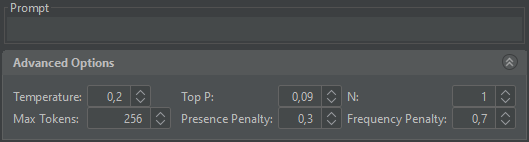
\includegraphics[width=0.9\textwidth]{chapter/chapter_4/wireframe-impl-ui-8+9}
  \caption{Textfeld für die Prompt und erweiterte Optionen.}
  \label{sec4:impl:par:ui-elements:fig:wireframe-ui-8+9}
\end{figure}

\lstinputlisting[style=java-code, caption={TextPanel-Klasse (Zweiter Teil)}, label={sec4:impl:par:ui-elements:lst:text-panel-p2}, firstnumber=35]{chapter/chapter_4/java/exp/text/TextPanel-P2.java}

\cref{sec4:impl:par:ui-elements:lst:text-panel-p2} zeigt den zweiten Teil der Klasse \textit{TextPanel} und die untere Schnittstelle \circitem{10}.
Dies ist im Fall der Klasse \textit{TextPanel} ein Textfeld für die generierte textuelle Erklärung und diese wird im Quellcode als Variable \textit{textResponseArea} eingeführt.
Zusätzlich wird ein Knopf \enquote{Generate Chat-Completion(s)} hinzugefügt und die Klasse als \textit{ActionListener} dem Knopf registriert.
Hierfür implementiert die Klasse \textit{TextPanel} das Interface \textit{ActionListener}.
Aufgabe des Knopfes ist das Erstellen und Verarbeiten einer Anfrage an den Endpunkt Text der OpenAI-Schnittstelle.
\cref{sec4:impl:par:ui-elements:fig:wireframe-text-complete} zeigt die vollständige Schnittstelle für die Klasse \textit{TextPanel}.

\begin{figure}[!ht]
  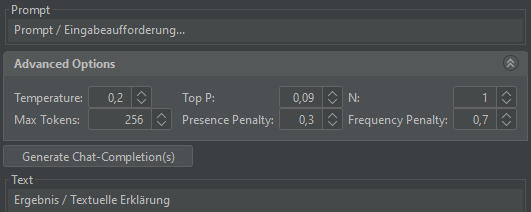
\includegraphics[width=0.9\textwidth]{chapter/chapter_4/wireframe-impl-text-complete}
  \caption{Vollständige Schnittstelle für die Klasse \textit{TextPanel}.}
  \label{sec4:impl:par:ui-elements:fig:wireframe-text-complete}
\end{figure}

\lstinputlisting[style=java-code, caption={TextPanel-Klasse (Letzter Teil)}, label={sec4:impl:par:ui-elements:lst:text-panel-p3}, firstnumber=49]{chapter/chapter_4/java/exp/text/TextPanel-P3.java}

\cref{sec4:impl:par:ui-elements:lst:text-panel-p3} zeigt den letzten Teil der Klasse \textit{TextPanel} und die für diese Klasse wichtigen Methoden \textit{setGraphCode}, \textit{setUpPrompt} und \textit{actionPerformed}.
Die Methode \textit{setGraphCode} hat die Verarbeitung eines Graph Codes zur Aufgabe und ruft hierfür wiederum die Methode \textit{setUpPrompt} auf.
Diese Methode ruft die Informationen in einem Graph Code ab und erstellt aus diesen eine Reihe an Textnachrichten, die zusammen eine Prompt darstellen.
Das Ergebnis dieses Aufrufs wird dann in einem dafür vorgesehenen Textfeld angezeigt.
In dieser Methode wird somit die Transformation von Graph Codes vorgenommen.
Die genauen Details der Implementierung dieser Methode werden daher in \cref{sec4:impl:subsubsec:gc-transformation} behandelt.
Schlussendlich hat die Methode \textit{actionPerformed} die Erzeugung einer Erklärung und der damit verbundenen Erzeugung einer Anfrage an den Endpunkt Text zur Aufgabe.
In dieser Methode wird somit die Integration des Endpunkts Text vorgenommen.
Genauere Details dieser Methode zum Erstellen einer Anfrage an den Endpunkt Text werden in \cref{sec4:impl:subsubsec:endpoint-integration} behandelt.

Im Folgenden zeigt \cref{sec4:impl:par:ui-elements:lst:image-panel} die Schnittstelle \textit{ImagePanel}.
\cref{sec4:impl:par:ui-elements:lst:image-panel} verhält sich dabei analog zu den \cref{sec4:impl:par:ui-elements:lst:text-panel-p1,sec4:impl:par:ui-elements:lst:text-panel-p2,sec4:impl:par:ui-elements:lst:text-panel-p3}.
Als solches ist die Schnittstelle \textit{ImagePanel} im Aufbau seiner Benutzeroberfläche, mit Außnahme der erweiterten Optionen und dem \textit{JLabel} + Icon zum Darstellen eines erzeugten Bildes im Vergleich zum Textfeld, identisch (siehe \cref{sec4:impl:subsubsec:ui:fig:wireframe-explanation-panel}).
Ein weiterer Unterschied besteht in der Methode \textit{actionPerformed} beim Generieren einer visuellen Erklärung zu einem Graph Code.
Hier wird zuerst eine spezielle, textuelle Erklärung generiert, die dann wiederum als Eingabe für den Endpunkt Bild zum Generieren einer visuellen Erklärung genutzt wird.
Genauere Details zum Erstellen einer Anfrage an den Endpunkt Bild werden in \cref{sec4:impl:subsubsec:endpoint-integration} behandelt.

\lstinputlisting[style=java-code, caption={ImagePanel-Klasse}, label={sec4:impl:par:ui-elements:lst:image-panel}, firstnumber=1]{chapter/chapter_4/java/exp/img/ImagePanel.java}

Damit sind beide Schnittstellen \textit{TextPanel} und \textit{ImagePanel} abschließend beschrieben und erklärt.
\cref{sec4:impl:par:ui-elements:fig:wireframe-image-complete} zeigt die vollständige Schnittstelle für die Klasse \textit{ImagePanel}.
Der Grundbereich \circitem{2}, \textit{ExplanationPanel}, ist damit abgeschlossen.

\begin{figure}[!ht]
  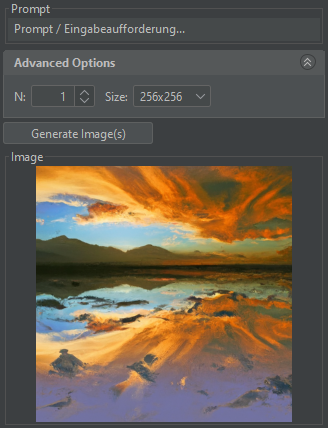
\includegraphics{chapter/chapter_4/wireframe-impl-image-complete}
  \caption{Vollständige Schnittstelle für die Klasse \textit{ImagePanel}.}
  \label{sec4:impl:par:ui-elements:fig:wireframe-image-complete}
\end{figure}

\FloatBarrier

Im weiteren Verlauf dieses Abschnitts wird in \cref{sec4:impl:par:ui-elements:lst:explainer-console} schlussendlich die Implementierung des letzten Grundbereichs \circitem{3}, \textit{ExplainerConsole}, behandelt und erklärt.
Die allgemeine Aufgabe des Grundbereichs \textit{ExplainerConsole} ist es wichtige Informationen über Prozesse des Programms zu loggen.
Wichtige Informationen können Bestätigungen von Aktionen und Fehlermeldungen umfassen.

\lstinputlisting[style=java-code, caption={ExplainerConsole-Klasse}, label={sec4:impl:par:ui-elements:lst:explainer-console}, firstnumber=1]{chapter/chapter_4/java/exc/ExplainerConsole.java}

Die Benutzeroberfläche des dritten Grundbereichs, \textit{ExplainerConsole}, besteht aus zwei nennenswerten Komponenten: Einem Textfeld für die angegebenen Informationen, sowie eine Toolbar mit Button zum Leeren des Textfeldes.
Das Textfeld ist eine Instanz der Klasse \textit{RSyntaxTextArea} und entstammt der gleichnamigen Abhängigkeit.
Die beiden Methoden \textit{onInsert} und \textit{onClear} sind Teil des eigens entwickelten Interfaces \textit{ITextInsertListener} und behandeln das Einfügen von Text in die Konsole, sowie das Leeren des Textfeldes der Konsole.

Damit sind alle Grundbereiche der Benutzeroberfläche des Programms abgeschlossen.
Der Zusammenschluss dieser Grundbereiche wird, wie bereits am Anfang des Abschnitts angemerkt, durch die Methode \textit{initComponents} in der Klasse \textit{ExplainerFrame} vorgenommen (siehe \cref{sec4:impl:par:ui-elements:lst:explainer-frame}).
Die genaue Implementierung dieser Methode kann in \cref{sec4:impl:par:ui-elements:lst:initComps} eingesehen werden und verdeutlicht den Zusammenschluss bzw. das Zusammenfügen der einzelnen Grundbereiche in das Fundament der gesamten Benutzungsschnittstelle.

\lstinputlisting[style=java-code, caption={Zusammenschluss der Grundbereiche}, label={sec4:impl:par:ui-elements:lst:initComps}, firstnumber=1]{chapter/chapter_4/java/methods/initComponents.java}

Besonders erwähnenswert für diese Methode ist die Komponente \textit{JXMultiSplitPane}, die Teil der Abhängigkeit \textit{SwingX} ist.
Zu dieser gehören ebenfalls die Komponenten \textit{MultiSplitLayout}, \textit{Split}, \textit{Divider} und \textit{Leaf}, die den Aufbau beschreiben.
Mithilfe der Komponente \textit{JXMultiSplitPane} können auf einfache Art und Weise und ohne großen Aufwand Schnittstellen angelegt werden, die in ihrer Größe anpassbar sind und die andernfalls nur durch aufwendige Verschachtelung mehrerer \textit{JSplitPane}'s erzeugt werden könnten.

In diesem Abschnitt wurde die Implementierung der Benutzeroberfläche beschrieben.
Hierfür wurden die Quellcodes für die in der Benutzeroberfläche verbauten Komponenten kompakt dargestellt und detailliert erläutert.
Eine abschließende Gesamtabbildung der vollständigen Benutzeroberfläche samt Beispielen kann im \cref{sec4:impl:subsec:summary} \enquote{Zusammenfassung} in den \cref{sec4:impl:subsubsec:summary-findings:fig:ui-ex-1,sec4:impl:subsubsec:summary-findings:fig:ui-ex-2,sec4:impl:subsubsec:summary-findings:fig:ui-ex-3} eingesehen werden.
Im folgenden Abschnitt wird die Interaktion mit und zwischen den in diesem Abschnitt beschriebenen Komponenten der Benutzeroberfläche thematisiert.

\FloatBarrier

\paragraph{Interaktion mit der Benutzeroberfläche}
\label{sec4:impl:par:ui-interaction}
In diesem Abschnitt wird die Implementierung der Interaktion zwischen Benutzern und Komponenten der Benutzeroberfläche genauer beschrieben.
Darüber hinaus werden auch die Zusammenhänge zwischen den Komponenten genauer betrachtet.
Dies umfasst Beschreibungen, wie die Komponenten gegenseitig miteinander interagieren und sich untereinander beeinflussen.
Die Beschreibung der Interaktion konzentriert sich dabei im Wesentlichen auf die Anwendungsfälle \hyperref[sec3:model:uc-1.1]{UC-1.1}, \hyperref[sec3:model:uc-1.2]{UC-1.2}, \hyperref[sec3:model:uc-1.3]{UC-1.3} und \hyperref[sec3:model:uc-1.5]{UC-1.5}.
Dies sind die Anwendungsfälle, in welchen Benutzer durch die Interaktion mit Komponenten in der Benutzeroberfläche komplexe und bedeutende Abläufe in Bezug auf Graph Codes in Gang setzen, die wiederum Einfluss auf andere Komponenten haben.
Allerdings sind von diesen Beschreibungen die verbleibenden Anwendungsfälle: \hyperref[sec3:model:uc-1.4]{UC-1.4} \enquote{Operation auswählen}, \hyperref[sec3:model:uc-1.7]{UC-1.7} \enquote{Erweiterte Optionen anpassen} (Interaktionen werden bereits durch jeweilige Komponenten bereitgestellt), \hyperref[sec3:model:uc-1.6]{UC-1.6} \enquote{Erklärungstyp umschalten} (Interaktion beeinflusst zwar die Komponente \textit{ExplanationPanel}, umfasst im Wesentlichen aber nur das Entfernen und Hinzufügen von \textit{ImagePanel} und \textit{TextPanel}) ausgenommen.
Der verbleibende Anwendungsfall \hyperref[sec3:model:uc-1.8]{UC-1.8} wird explizit in \cref{sec4:impl:subsubsec:endpoint-integration} behandelt.

\cref{sec4:impl:par:ui-interaction:lst:import-gcs} zeigt das Steuerelement \textit{ImportGraphCodesController}, welches mit dem Anwendungsfall \hyperref[sec3:model:uc-1.1]{UC-1.1} \enquote{Graph Code(s) importieren} assoziiert ist.
Das Steuerelement wird durch einen Klick auf den Knopf \enquote{Import Graph Code(s)} initiiert und importiert ein oder mehrere aus einem Auswahldialog ausgewählte Graph Code Dateien in die Liste für Graph Codes (siehe \cref{sec3:model:par:wireframe:fig:stage-2+3} \circitem{5}).

\lstinputlisting[style=java-code, caption={ImportGraphCodesController-Klasse}, label={sec4:impl:par:ui-interaction:lst:import-gcs}, firstnumber=1]{chapter/chapter_4/java/interaction/ImportGraphCodesController.java}

Der Auswahldialog wird, wie auch bereits in \cref{sec3:model:par:mechanism-use-cases:fig:mech-uc-1.1} identifiziert, durch die Komponente \textit{JFileChooser} bereitgestellt.
Durch eine Anpassung des Verzeichnisses zeigt der Dialog relativ auf das Verzeichnis des Projekts, in welchem Graph Code Dateien gespeichert sind.
Weitere Anpassungen des Dialogs umfassen einen Dateifilter, sodass Benutzern nur Dateien mit der Endung \enquote{.gc} angezeigt werden bzw. nur diese ausgewählt werden können, sowie eine mögliche Mehrfachauswahl von Dateien.
Werden die ausgewählten Dateien geöffnet, so werden für alle ausgewählten Dateien Einträge (\textit{GraphCodeListElement}) für die Liste geschaffen, die dann dem Datenmodell (\textit{DefaultListModel}) der Liste hinzugefügt werden.

Damit entspricht der Ablauf der Aktionen in \cref{sec4:impl:par:ui-interaction:lst:import-gcs} grundsätzlich den modellierten Abläufen im UML-Sequenzdiagramm, dargestellt in \cref{sec3:model:par:seq-use-cases:fig:seq-diag-uc-1.1}, für den Anwendungsfall \hyperref[sec3:model:uc-1.1]{UC-1.1}.

% Steuerelement: Durch welche Interaktion wird diese Aktion iniiert? -> Benutzer muss auf Knopf ... klicken.
% Dann beschreiben, wie der Ablauf der Aktionen aussieht... und diese mit der Modellierung vergleichen?
% Hier auf die notwendigen Komponenten dieser Aktionen

% Schritt für Schritt dann den Ablauf der Aktionen beschreiben...
% Für jede Aktionen betrachten, ob es sinnvoll oder notwendig ist auf die an dieser Aktion beteiligten Komponenten einzugehen...
% Wenn ja, dann auf jeweilige Komponenten verweisen und auch auf die Identifizierung dieser Komponenten in Mechanismen verweisen...
% Später dann den Ablauf der Aktionen mit dem in der Modellierung entsprechendem Sequenzdiagramm "vergleichen"...

\cref{sec4:impl:par:ui-elements:lst:remove-gcs} zeigt das Steuerelement \textit{RemoveSelectedGraphCodesController}, welches mit dem Anwendungsfall \hyperref[sec3:model:uc-1.2]{UC-1.2} \enquote{Graph Code(s) entfernen} assoziiert ist.
Das Steuerelement wird durch einen Klick auf den Knopf \enquote{Remove selected Graph Code(s)} initiiert und entfernt die in der Liste ausgewählten Graph Codes.

\lstinputlisting[style=java-code, caption={RemoveSelectedGraphCodesController-Klasse}, label={sec4:impl:par:ui-elements:lst:remove-gcs}, firstnumber=1]{chapter/chapter_4/java/interaction/RemoveSelectedGraphCodesController.java}

Voraussetzung für das erfolgreiche Entfernen von ein oder mehreren Graph Code Datei(en) ist, dass die Liste einen oder mehrere Graph Code(s) enthält bzw. diese von einem Benutzer ausgewählt worden sind.
Hierfür wird die Liste und das Datenmodell der Liste benötigt.
In einem ersten Schritt werden die Indizes von potentiell ausgewählten Einträgen der Liste abgefragt und geprüft, ob die Anzahl der ausgewählten Einträge größer null ist.
Sofern dies der Fall ist, werden diese Indizes durchlaufen und dem Datenmodell mitgeteilt, dass der Eintrag am entsprechenden Index entfernt werden soll.

Damit entspricht der Ablauf der Aktionen in \cref{sec4:impl:par:ui-elements:lst:remove-gcs} ebenfalls grundsätzlich den modellierten Abläufen im UML-Sequenzdiagramm, dargestellt in \cref{sec3:model:par:seq-use-cases:fig:seq-diag-uc-1.2}, für den Anwendungsfall \hyperref[sec3:model:uc-1.2]{UC-1.2}.

\cref{sec4:impl:par:ui-elements:lst:select-gcs} zeigt das Steuerelement \textit{GraphCodeSelectionListener}, welches mit dem Anwendungsfall \hyperref[sec3:model:uc-1.3]{UC-1.3} \enquote{Graph Code(s) auswählen} assoziiert ist.
Das Steuerelement wird durch die Auswahl eines oder mehrerer Elemente in der Liste initiiert und beeinflusst daraufhin durch Initiierung weiterer Aktionen andere Benutzungsschnittstellen, indem Informationen an diese weitergegeben werden.

\lstinputlisting[style=java-code, caption={GraphCodeSelectionListener-Klasse}, label={sec4:impl:par:ui-elements:lst:select-gcs}, firstnumber=1]{chapter/chapter_4/java/interaction/GraphCodeSelectionListener.java}

Voraussetzung für das erfolgreiche Auswählen von ein oder mehreren Graph Code Datei(en) ist, dass die Liste einen oder mehrere Graph Code(s) enthält.
Ist ein Eintrag aus der Liste ausgewählt, so können andere Benutzungsschnittstellen über die Informationen in diesem Eintrag informiert und angepasst werden.
Die Informationen eines Eintrages umfassen den aus der Datei gelesenen Graph Code und den Dateinamen.
Zu den angepassten Benutzungsschnittstellen gehören somit die Tabelle zur Darstellung des Graph Codes \textit{GraphCodeTable} inklusive eines Textfeldes zur Anzeige des Dateinamens, sowie die Schnittstelle \textit{ExplanationPanel} zur Erzeugung von Erklärungen.
Die Informationen eines ausgewählten Eintrages werden hierbei jeweils an \textit{GraphCodeTable} und \textit{ExplanationPanel} delegiert, woraufhin diese in den entsprechenden Komponenten weiterverarbeitet werden.

Damit entspricht der Ablauf der Aktionen in \cref{sec4:impl:par:ui-elements:lst:select-gcs} ebenfalls grundsätzlich den modellierten Abläufen im UML-Sequenzdiagramm, dargestellt in \cref{sec3:model:par:seq-use-cases:fig:seq-diag-uc-1.3}, für den Anwendungsfall \hyperref[sec3:model:uc-1.3]{UC-1.3}.

\cref{sec4:impl:par:ui-elements:lst:mouse-gcs} zeigt das Steuerelement \textit{GraphCodeListMouseAdapter}.
Dieses Steuerelement ist nicht explizit mit einem Anwendungsfall assoziiert und wird durch eine Interaktion der Maus mit der Liste initiiert.
Ist diese Interaktion ein Doppelklick, so wird in der Liste geprüft, ob an der Position der Interaktion ein Eintrag vorliegt.
Sofern dies der Fall ist, wird der Index dieses Eintrags bestimmt und der Eintrag aus dem Datenmodell \textit{DefaultListModel} extrahiert.
Dem Benutzer wird dann ein Dialog angezeigt, mit welchem dieser eine Umbenennung des Eintrags vornehmen kann.

\lstinputlisting[style=java-code, caption={GraphCodeListMouseAdapter-Klasse}, label={sec4:impl:par:ui-elements:lst:mouse-gcs}, firstnumber=1]{chapter/chapter_4/java/interaction/GraphCodeListMouseAdapter.java}

Neben dem Steuerelement \textit{GraphCodeListMouseAdapter} wird der Liste noch ein weiteres Steuerelement hinzugefügt bzw. registriert.
Dieses Steuerelement heißt \textit{ListItemTransferHandler} und ermöglicht das Verschieben von Einträgen mittels Drag und Drop.
% Der Quellcode für diese und weitere Komponenten kann in ... eingesehen werden.

\cref{sec4:impl:par:ui-elements:lst:calculate-gcs-p1,sec4:impl:par:ui-elements:lst:calculate-gcs-p2,sec4:impl:par:ui-elements:lst:calculate-gcs-p3,sec4:impl:par:ui-elements:lst:calculate-gcs-p4,sec4:impl:par:ui-elements:lst:calculate-gcs-p5} zeigen das Steuerelement \textit{GraphCodeCalculationController}, welches mit dem Anwendungsfall \hyperref[sec3:model:uc-1.5]{UC-1.5} \enquote{Operation ausführen} assoziiert ist.
Das Steuerelement wird durch einen Klick auf den Knopf \textit{Execute} initiiert und führt die in Anwendungsfall \hyperref[sec3:model:uc-1.4]{UC-1.4} ausgewählte Operation auf den ausgewählten Graph Codes aus.

\cref{sec4:impl:par:ui-elements:lst:calculate-gcs-p1} zeigt die für die Anwendung von Operationen auf Graph Codes notwendigen Komponenten.
Dies umfasst die in Anwendungsfall \hyperref[sec3:model:uc-1.4]{UC-1.4} ausgewählte Operation \textit{actionItem}, die in den folgenden \cref{sec4:impl:par:ui-elements:lst:calculate-gcs-p2,sec4:impl:par:ui-elements:lst:calculate-gcs-p3,sec4:impl:par:ui-elements:lst:calculate-gcs-p4,sec4:impl:par:ui-elements:lst:calculate-gcs-p5} in einem Switch-Statement zur Differenzierung der auszuführenden Aktionen dienen wird, sowie eine Liste \textit{selGraphCodes} der ausgewählten Einträge aus der Liste.

\lstinputlisting[style=java-code, caption={GraphCodeCalculationController-Klasse}, label={sec4:impl:par:ui-elements:lst:calculate-gcs-p1}, firstnumber=1]{chapter/chapter_4/java/interaction/GraphCodeCalculationController-P1.java}

\cref{sec4:impl:par:ui-elements:lst:calculate-gcs-p2} zeigt die Anwendung der Operation \enquote{Union}.
Die Operation zur Berechnung der Vereinigung von Graph Codes wird bereits vom GMAF durch die Komponente \textit{GraphCodeCollection} bereitgestellt.
Um diese Operation nutzen zu können, muss in einem ersten Schritt aus der Liste an Einträgen eine Liste an Graph Codes geschaffen werden.
Dies wird durch das Abbilden eines Eintrages auf einen Graph Code erreicht.
Weiter wird die Liste in einen Vektor umgewandelt, da die Funktion der Vereinigung einen Vektor als Eingabe erwartet.
Die Ausgabe der Vereinigung ist wiederum ein Graph Code, welcher dann in einen neu erstellten Eintrag eingebettet wird.
Über einen Dialog kann dann ein Benutzer nach Anwendung der Operation dem Eintrag einen neuen Namen zuweisen.
Der Eintrag wird dann dem Datenmodell der Liste hinzugefügt.

\lstinputlisting[style=java-code, caption={GraphCodeCalculationController-Klasse}, label={sec4:impl:par:ui-elements:lst:calculate-gcs-p2}, firstnumber=1]{chapter/chapter_4/java/interaction/GraphCodeCalculationController-P2.java}

\cref{sec4:impl:par:ui-elements:lst:calculate-gcs-p3} zeigt die Anwendung der Operation \enquote{Subtraction}.
Auch die Operation zur Berechnung der Subtraktion eines Graph Codes von einem anderen Graph Code wird durch die Komponente \textit{GraphCodeCollection} bereitgestellt.
Im Fall dieser Operation wird aus den ausgewählten Eintrag allerdings nur der erste und zweite Eintrag berücksichtigt.
Ausgabe der Operation der Subtraktion ist ebenfalls ein Graph Code.
Die verbleibenden Aktionen verhalten sich analog zur Operation der Vereinigung von Graph Codes.

\clearpage

\lstinputlisting[style=java-code, caption={GraphCodeCalculationController-Klasse}, label={sec4:impl:par:ui-elements:lst:calculate-gcs-p3}, firstnumber=1]{chapter/chapter_4/java/interaction/GraphCodeCalculationController-P3.java}

\cref{sec4:impl:par:ui-elements:lst:calculate-gcs-p4} zeigt die Anwendung der Operation \enquote{Similarities}.
Die Operation zur Berechnung der Gemeinsamkeiten von Graph Codes wurde bereits in \cref{sec3:model:par:mechanism-use-cases:alg:sim} als Teil der Modellierung in einem Pseudoalgorithmus vorgestellt.
Die Implementierung dieses Algorithmus ist in \cref{sec4:impl:par:ui-elements:lst:calculate-sim} einsehbar und wird ähnlich wie die Operationen zur Vereinigung und Subtraktion in die Klasse \textit{GraphCodeCollection} eingebunden.

\lstinputlisting[style=java-code, caption={GraphCodeCalculationController-Klasse}, label={sec4:impl:par:ui-elements:lst:calculate-gcs-p4}, firstnumber=1]{chapter/chapter_4/java/interaction/GraphCodeCalculationController-P4.java}

\lstinputlisting[style=java-code, caption={Algorithmus zur Bestimmung der Gemeinsamkeiten von Graph Codes}, label={sec4:impl:par:ui-elements:lst:calculate-sim}, firstnumber=1]{chapter/chapter_4/java/algorithm/Alg-Similarities.java}

Die für die Anwendung der Operation \enquote{Similarities} notwendigen Schritte sind äquivalent zu den Schritten der Operation der Vereinigung, mit Ausnahme des Aufrufs der spezifischen Funktion, deren Schritte im Weiteren genauer beschrieben werden.

In einem ersten Schritt wird in Zeile 5 die Vereinigung aller Graph Codes berechnet.
Ergebnis ist ein Graph Code mit einem Wörterbuch, welches alle Merkmale aller Graph Codes enthält.
In einem weiteren Schritt werden von Zeile 11 bis 13 alle Graph Codes in einer Schleife durchlaufen.
Bei jedem Durchlauf werden alle Elemente aus dem Wörterbuch der Vereinigung entfernt, die nicht in irgendeinem Wörterbuch der anderen Graph Codes vorhanden sind.
Hierzu wird in Zeile 7 eine Kopie des Wörterbuchs erstellt und später verwendet.
Übrig bleiben alle Elemente, die auch in den Wörterbüchern aller anderen Graph Codes vorkommen.
Dieses Wörterbuch wird dann dem Ergebnis zugewiesen.
Von Zeile 18 bis 30 werden dann in einem letzten Schritt für alle Graph Codes alle Elemente zeilen- und spaltenweise durchlaufen, um die Werte für diese Einträge zu bestimmen und dem Ergebnis zuzuweisen.
Schlussendlich ist das Ergebnis dieser Funktion ein Graph Code, dessen Wörterbuch alle gemeinsamen Elemente bzw. Merkmale und Werte aller verarbeiteten Graph Codes enthält.
Auf die Modellierung rückblickend ist die Implementierung dieses Algorithmus somit sehr ähnlich zu dem konzipierten Pseudoalgorithmus.

\cref{sec4:impl:par:ui-elements:lst:calculate-gcs-p5} zeigt die Anwendung der Operation \enquote{Differences}.
Die Operation zur Berechnung der Unterschiede von Graph Codes wurde bereits in \cref{sec3:model:par:mechanism-use-cases:alg:dif} als Teil der Modellierung in einem Pseudoalgorithmus vorgestellt.
Die Implementierung dieses Algorithmus ist in \cref{sec4:impl:par:ui-elements:lst:calculate-diff} einsehbar und wird ebenfalls in die Klasse \textit{GraphCodeCollection} eingebunden.

\lstinputlisting[style=java-code, caption={GraphCodeCalculationController-Klasse}, label={sec4:impl:par:ui-elements:lst:calculate-gcs-p5}, firstnumber=1]{chapter/chapter_4/java/interaction/GraphCodeCalculationController-P5.java}

\lstinputlisting[style=java-code, caption={Algorithmus zur Bestimmung der Unterschiede von Graph Codes}, label={sec4:impl:par:ui-elements:lst:calculate-diff}, firstnumber=1]{chapter/chapter_4/java/algorithm/Alg-Differences.java}

Die für die Anwendung der Operation \enquote{Differences} notwendigen Schritte sind ebenfalls äquivalent zu den Schritten der Operation der Vereinigung, mit Ausnahme des Aufrufs der spezifischen Funktion.

Der in \cref{sec4:impl:par:ui-elements:lst:calculate-diff} dargestellte Algorithmus zur Berechnung der Unterschiede von Graph Codes ist dabei nahezu identisch mit dem in \cref{sec4:impl:par:ui-elements:lst:calculate-sim} dargestellten Algorithmus zur Berechnung der Gemeinsamkeiten.
Folglich ist die Implementierung dieses Algorithmus ebenfalls sehr ähnlich zu dem entsprechend konzipierten Pseudoalgorithmus.
Der bedeutende Unterschied besteht in der Art der Berechnung des Wörterbuchs.
Genauer ist die Differenz aller Graph Codes die Vereinigung aller Graph Codes abzüglich der Gemeinsamkeiten aller Graph Codes.
Die Berechnung dieser Differenz geschieht in Zeile 17 und nutzt hierfür die Abhängigkeit \textit{Guava} von Google.
Die Methode \textit{difference} erwartet als Eingabe zwei Sets.
Dies kann ein Problem darstellen, da ein Set nicht die Ordnung bzw. Reihenfolge seiner Elemente beibehält, diese aber für das Wörterbuch eines Graph Codes besonders wichtig ist.
Daher werden in diesem Fall die Wörterbücher in ein \textit{LinkedHashSet} übernommen, welche die Reihenfolge ihre Elemente beibehalten.
Diese werden dann als Eingabe für die Funktion benutzt.

In diesem Abschnitt wurde die Implementierung der Interaktion zwischen Benutzern des GMAF und den Komponenten der Benutzeroberfläche genauer beschrieben.
Es wurden die an dieser Interaktion beteiligten Steuerelemente vorgestellt und beschrieben, welche Aktionen diese Steuerelemente jeweils durchführen und wie diese die Verarbeitung oder die Benutzeroberfläche beeinflussen.
Im nächsten Abschnitt werden die Erkenntnisse aus den Abschnitten dieses Forschungsziels zusammengefasst, diskutiert und eingeordnet.

\clearpage

\subsubsection{Diskussion}
\label{sec4:impl:subsubsec:fz1:discussion}
Der Modellierung nach orientiert, wurde in \cref{sec4:impl:par:ui-elements} die Implementierung der Benutzungsschnittstelle genauer beschrieben.
Dies umfasst eine genauere Beschreibung des in Bereiche aufgeteilten Aufbaus der Benutzeroberfläche.
Die Implementierung der in diesen Bereichen enthaltenen Komponenten wurde dabei mit kompaktem Quellcode dokumentiert und beschrieben.
Des Weiteren wurden in der Beschreibung dieser Komponenten Vergleiche bzw. Assoziationen zu den Anwendungsfällen und Mechanismen aus der Modellierung gemacht.
In \cref{sec4:impl:par:ui-elements} wurde somit der Bereich \textit{View} behandelt.
Allerdings konnten die Methoden \textit{setUpPrompt} und \textit{actionPerformed} in \cref{sec4:impl:par:ui-elements:lst:text-panel-p3,sec4:impl:par:ui-elements:lst:image-panel}.

Anhand dieser Komponenten wurde dann in \cref{sec4:impl:par:ui-interaction} die Implementierung der Interaktion zwischen den Benutzern des GMAF und den Komponenten der Benutzeroberfläche, sowie die Interaktion zwischen den Komponenten untereinander genauer beschrieben.
Hierfür wurden die Komponenten für die Interaktion, auch Steuerelemente genannt, mit kompaktem Quellcode dokumentiert und beschrieben.
In \cref{sec4:impl:par:ui-interaction} wurde somit der Bereich \textit{Controller} behandelt.

In diesem Abschnitt wurden allerdings die Methoden \textit{setUpPrompt} und \textit{actionPerformed}, jeweils aus den \cref{sec4:impl:par:ui-elements:lst:text-panel-p3,sec4:impl:par:ui-elements:lst:image-panel} ausgelassen.
Diese Methoden dienen zur Vorbereiten einer Prompt bzw. der Interaktion zur Erstellung einer Anfrage an einen Endpunkt und wurden explizit in diesem Forschungsziel ausgelassen und werden separat im zweiten \hyperref[sec4:impl:subsec:fz-integration]{Forschungsziel \enquote{Integration generativer KI in das GMAF}} behandelt.
% Genauer wird die Methode \textit{setUpPrompt} in \cref{sec4:impl:subsubsec:gc-transformation} und \textit{actionPerformed} in \ref{sec4:impl:subsubsec:endpoint-integration} behandelt.

% Es wäre auch sinnvoll? in diese Diskussion die Abarbeitung der offenen Herausforderungen einfließen zu lassen...
% Bezüglich dieses Abschnitts bzw. dieses FZs konnte die offene Herausforderung OH 1.2 abgedeckt werden...


\subsection{FZ 2.3/I Integration generativer KI in das GMAF}
\label{sec4:impl:subsec:fz-integration}
% Einleitung in FZ 2.3/I +
% Strukturelle Einleitung...

\subsubsection{Umsetzung der Transformation von Graph Codes}
\label{sec4:impl:subsubsec:gc-transformation}

\subsubsection{Integration der Endpunkte}
\label{sec4:impl:par:endpoint-integration}

\clearpage

\subsection{Zusammenfassung}
\label{sec4:impl:subsec:summary}
% Einleitung zur Zusammenfassung
In diesem Kapitel wurde die Implementierung behandelt.
Im Folgenden werden die wesentlichen Ergebnisse und Erkenntnisse der Implementierung nach den Forschungszielen der Implementierungsphase, wie nach der Methodik nach Nunamaker vorgesehen, aufgeschlüsselt und in \cref{sec4:impl:subsubsec:summary-findings} in ... kurz zusammengefasst.

\subsubsection{Gewonnene Erkenntnisse}
\label{sec4:impl:subsubsec:summary-findings}
% Abbildungen und Screenshots zeigen das Ergebnis der Proof-of-Concept Implementierung. Screenshots werden beschrieben und erklärt.
% In ... (Tab) werden dann die Ergebnisse aufgeschlüsselt und in Tabelle zusammengefasst.

\subsubsection{Weiteres Vorgehen}
\label{sec4:impl:subsubsec:further-approach}

\begingroup
\def\arraystretch{1.1}%
\begin{xltabular}{\linewidth}{
            @{}
            >{
                \hsize=0.2\linewidth
                \raggedright\arraybackslash
            }X
            >{
                \hsize=0.6\linewidth
                \raggedright\arraybackslash
            }X
            >{
                \hsize=0.2\linewidth
            }X
            @{}
        }

        % First Header

        \caption{Tabelle zur Übersicht des aktuellen Arbeitstands.}
        \label{sec4:impl:subsec:summary:table:summary}
        \\

        \toprule
        \multicolumn{3}{
            >{
                    \hsize=\linewidth\centering\arraybackslash
            }X
        }
        {
            \textbf{Forschungsziele}
        } \\ \midrule
        \textbf{FZ / OH} &  \textbf{Beschreibung} & \textbf{Referenz} \\ \midrule

        \endfirsthead

        \toprule
        \multicolumn{3}{
            >{
                    \hsize=\linewidth\centering\arraybackslash
            }X
        }
        {
            \textbf{Forschungsziele}
        } \\ \midrule
        \textbf{FZ / OH} & \textbf{Beschreibung} & \textbf{Referenz} \\ \midrule

        \endhead

        % Lower Rows

        \multicolumn{3}{
            >{
                    \hsize=\linewidth\centering\arraybackslash
            }X
        }
        {
            \textbf{Erklärbarkeit von MMIR mittels generativer KI}
        }
        \\
        \midrule

        FZ 1.1/O
        &
        Recherche zur Erklärbarkeit von MMIR mittels generativer KI
        \\

        &
        Grundlegende Technologien:
        &

        \\

        &
        \tabitem GMAF
        &
        \cref{sec2:sota:subsubsec:gmaf}
        \\

        &
        \tabitem MMFG
        &
        \cref{sec2:sota:subsubsec:mmfg}
        \\

        &
        \tabitem Graph Code
        &
        \cref{sec2:sota:subsubsec:graph-codes}
        \\

        % Offene Herausforderungen aus FZ1/O

        OH 1.1
        &
        Erste offene Herausforderung
        &
        \hyperref[sec2:sota:oi:1.1]{\textbf{OH 1.1}}
        \\


        &
        Systeme generativer KI und ein Überlick über aktuelle Systeme
        &
        \cref{sec2:sota:subsubsec:genai}
        \\

        &
        Diskussion und Auswahl von Systemen
        &
        \cref{sec2:sota:subsubsec:fz1:discussion}
        \\

        OH 1.2
        &
        Zweite offene Herausforderung
        &
        \hyperref[sec2:sota:oi:2.1]{\textbf{OH 2.1}}
        \\

        \midrule

        FZ 1.2/TB
        &
        Modellierung der Erklärbarkeit von MMIR mittels generativer KI
        &

        \\

        &
        Erklärbarkeit durch generative KI
        &
        \cref{sec3:model:subsubsec:explainability-through-genai}
        \\

        &
        $\rightarrow$ Behandlung der ersten offenen Herausforderung \hyperref[sec2:sota:oi:1.1]{\textbf{OH 1.1}}
        &
        \\

        &
        Anwendungsfälle:
        &
        \cref{sec3:model:subsubsec:use-cases}
        \\

        &
        \tabitem Textuelle Beschreibungen
        &
        %\cref{sec3:model:par:textual-desc-use-cases}
        \\

        &
        \tabitem Wireframes
        &
        %\cref{sec3:model:par:wireframe}
        \\

        &
        \tabitem Mechanismen
        &
        %\cref{sec3:model:par:mechanism-use-cases}
        \\

        &
        \tabitem Sequenzdiagramme
        &
        %\cref{sec3:model:par:seq-use-cases}
        \\

        &
        $\rightarrow$ Behandlung der zweiten offenen Herausforderung \hyperref[sec2:sota:oi:1.2]{\textbf{OH 1.2}}
        &
        \\

        \midrule

        FZ 1.3/I
        &
        Implementierung der Erklärbarkeit von MMIR mittels generativer KI
        &

        \\

        \midrule

        FZ 1.4/E
        &
        Evaluierung der Erklärbarkeit von MMIR mittels generativer KI
        &

        \\

        \midrule

        \multicolumn{3}{
            >{
                    \hsize=\linewidth\centering\arraybackslash
            }X
        }
        {
            \textbf{Integration generativer KI in das GMAF}
        }
        \\
        \midrule

        FZ 2.1/O
        &
        Recherche zur Integration generativer KI in das GMAF
        &

        \\


        &
        Aufzeigen der Integrationsmöglichkeiten von:
        &

        \\

        &
        \tabitem Graph Codes
        &
        \cref{sec2:sota:subsubsec:gc-capabilities-integration}
        \\

        &
        Erste offene Herausforderung
        &
        \hyperref[sec2:sota:oi:2.1]{\textbf{OH 2.1}}
        \\

        &
        \tabitem Systemen generativer KI
        &
        \cref{sec2:sota:subsubsec:genai-capabilities-integration}
        \\

        &
        Zweite offene Herausforderung
        &
        \hyperref[sec2:sota:oi:2.2]{\textbf{OH 2.2}}
        \\

        \midrule

        FZ 2.2/TB
        &
        Modellierung der Integration generativer KI in das GMAF
        &

        \\

        &
        Transformation von Graph Codes
        &
        \cref{sec3:model:subsubsec:gc-transformation}
        \\

        &
        \tabitem Transformation des Vokabulars
        &
        \\

        &
        \tabitem Transformation der Matrix
        &
        \\

        &
        \tabitem Anwendung von Graph Code Metriken
        &
        \\

        &
        $\rightarrow$ Behandlung der ersten offenen Herausforderung \hyperref[sec2:sota:oi:2.1]{\textbf{OH 2.1}}
        &
        \\

        &
        Einbindung generativer KI in das GMAF
        &
        \cref{sec3:model:subsubsec:genai-integration}
        \\

        &
        $\rightarrow$ Behandlung der zweiten offenen Herausforderung \hyperref[sec2:sota:oi:2.2]{\textbf{OH 2.2}}
        &
        \\

        \midrule

        FZ 2.3/I
        &
        Implementierung der Integration generativer KI in das GMAF
        &

        \\

        \midrule

        FZ 2.4/E
        &
        Evaluierung der Integration generativer KI in das GMAF
        &

        \\

        \bottomrule
\end{xltabular}
\endgroup



\section{Evaluierung}
\label{sec5:eval}
In diesem Kapitel werden die Ergebnisse der Forschungsziele der vorangegangenen Phasen
\begin{itemize}
  \item Beobachtungsphase, \cref{sec2:sota} \enquote{Stand der Wissenschaft und Technik}
  \item Theoriebildungsphase, \cref{sec3:model} \enquote{Modellierung}
  \item Implementierungsphase, \cref{sec4:impl} \enquote{Implementierung}
\end{itemize}
im Vergleich zu den in \cref{sec1:intro:subsec:research-questions} identifizierten, initialen Forschungsfragen in einer detaillierten Evaluierung überprüft.
Ziel der Evaluierung ist es, Erkenntnisse zur Vollständigkeit, sowie Korrektheit der prototypischen Software für die Prototypen der Benutzungsschnittstelle(n) und Funktionen der Anwendung zu erlangen.
Dieses Ziel ergibt sich aus der in diesem Kapitel gewählten Methodik der Evaluierung, sowie aus den Forschungszielen vom Typ Experiment und folgt dem Ansatz nach Nunamaker \cite{nunamaker}.
Zudem werden konkrete Ziele der Evaluierung, Auswahl von Methoden der Evaluierung, um diese Ziele zu erreichen, sowie die Vorbereitung, Durchführung und Auswertung von Experimenten nach den gewählten Methoden der Evaluierung, beschrieben.
Mit diesem Ansatz werden alle Problembereiche im Vergleich zu den initialen Forschungszielen zufriedenstellend und ausführlich abgedeckt.

Die Gliederung des Kapitels lautet wie folgt:
\cref{sec5:eval:subsec:eval-goals-methodology} konkretisiert die Ziele und zu beantwortenden Fragestellungen der Evaluierung.
Des Weiteren wird für die Evaluierung eine geeignete Evaluierungsmethodik gewählt und erläutert.
In \cref{sec5:eval:subsec:assign-exper} werden die in der Evaluierung durchzuführenden Experimente formuliert, sowie den entsprechenden Forschungszielen zugeordnet.
In \cref{sec5:eval:subsec:fz-explainability,sec5:eval:subsec:fz-integration} werden jeweils die Vorbereitung, Durchführung und die Ergebnisse der jeweiligen Experimente beschrieben.
In \cref{sec5:eval:subsec:adaptation} werden in Abhängigkeit der in den Experimenten potentiell entdeckten Mängel, Fehlerbehandlungen beschrieben.
In \cref{sec5:eval:subsec:summary} werden dann die Ergebnisse der Evaluierung zusammengefasst und diskutiert.

\subsection[Ziele der Evaluierung und geeignete Evaluierungsmethodik]{\texorpdfstring{Ziele der Evaluierung und geeignete \\ Evaluierungsmethodik}{Ziele der Evaluierung und geeignete Evaluierungsmethodik}}
\label{sec5:eval:subsec:eval-goals-methodology}
Wesentliches Ziel der Evaluierung ist die Sicherstellung der Funktionalität der entwickelten, prototypischen Proof-of-Concept Implementierung.
In diesem Abschnitt werden die konkreten Ziele der Evaluierung formuliert, auf deren Basis eine geeignete Evaluierungsmethodik ausgewählt wird.
Konkrete Ziele lassen sich aus den Forschungszielen vom Typ Experiment ableiten.
Folgende konkrete Ziele können dabei formuliert werden:
Bewertung der \undline{Vollständigkeit} und \undline{Korrektheit} der prototypischen Proof-of-Concept Implementierung in Bezug auf die in \cref{sec3:model} \enquote{Modellierung} entwickelten Konzepte.
Diese Ziele stellen die Grundlage für die Auswahl einer Evaluierungsmethodik dar.
Durch Gruppierung und Zuweisung dieser Ziele zu einem Experiment können mehrere Ziele in einer Durchführung eines Experiments abgedeckt werden.
Aus diesen festgelegten, konkreten Zielen ergibt sich folgendes Ziel der Evaluierung, für dessen Erreichen Experimente entworfen werden, die nach ihrer Durchführung Erkenntnisse bezüglich der Vollständigkeit und Korrektheit der prototypischen Proof-of-Concept Implementierung der Software zulassen.

In \cref{sec2:sota:subsec:eval-methodology} wurden Methodiken vorgestellt, mit welchen eine systematische Evaluierung einer Anwendung möglich ist.
Mittels dieser Methodiken können Aussagen und Bewertungen zur entwickelten Software vorgenommen werden.
Es gilt aus der Sammlung dieser Methodiken eine geeignete Methodik zu wählen, die mit den in diesem Projekt begrenzten Ressourcen und Möglichkeiten zur Verfügung stehen und mit welcher möglichst viele formulierten Ziele erreicht werden können.
Ein weiterer wichtiger Aspekt, den es bei der Auswahl eines geeigneten Evaluierungsverfahrens bzw. -methodik zu beachten gilt, ist, dass es sich bei der zu evaluierenden Software nicht um ein fertiges, einsetzbares Softwareprodukt handelt, sondern nur um eine prototypische Proof-of-Concept Implementierung.
Da im Rahmen der Implementierung ein praktisch, benutzbarer Softwareprototyp entwickelt wurde, bietet es sich an, genau diesen Prototyp zur Evaluierung zu verwenden, sodass sich die Erkenntnisse und Ergebnisse der Evaluierung auf den aktuellsten Stand der Software und somit auch dieser Arbeit beziehen.

% Für die Durchführung kann auf einen Experten zurückgegriffen werden... (S.W.)
Für die Durchführung der Evaluierung kann auf einen Experten des Lehrgebiets Multimedia und Internetanwendungen zurückgegriffen werden.
Aus den verfügbaren Evaluierungsmethodiken wird im Folgenden der Cognititve Walkthrough gewählt.
Der Cognititve Walkthrough generiert keine Erkenntnisse bezüglich der Effektivität einer Anwendung, bietet sich jedoch trotzdem zur Evaluierung an, da dieser einfach, kostengünstig und mit limitierten Ressourcen durchführbar ist.
Im Verfahren des Cognititve Walkthrough werden systematisch atomare Aktionen durchlaufen.
Diese atomaren Aktionen sind Aufgaben, die ein Benutzer ausführen muss, um sein angestrebtes Ziel zu erreichen, und lassen sich aus den entsprechenden Interaktionen eines Benutzers mit dem System, festgehalten in \cref{sec3:model:par:mechanism-use-cases} \enquote{Anwendungsfällen}, ableiten.
Mit diesem Vorgehen wird sich versprochen, gezielt Erkenntnisse zu den Zielen \enquote{Bewertung der Vollständigkeit und Korrektheit} zu erlangen.
Andere umfangreichere Evaluierungsmethodiken sind im Rahmen dieser Arbeit nicht anwendbar aufgrund mangelnder zeitlicher, sowie personeller Ressourcen.

Im weiteren Verlauf dieses Kapitels wird ein Cognititve Walkthrough geplant, in seiner Durchführung beschrieben und schlussendlich anhand der gewonnenen Erkenntnisse ausgewertet.
Ziel der Durchführung eines Cognititve Walkthrough ist es, neue Erkenntnisse zur Funktionalität der entwickelten Anwendung durch Bewertung der Vollständigkeit und Korrektheit zu erlangen.
Hierfür wird im nächsten Abschnitt eine Wahl und Zuweisung der in der Evaluierung durchzuführenden Experimente vorgenommen.

\subsection{Wahl und Zuweisung durchzuführender Experimente}
\label{sec5:eval:subsec:assign-exper}
In Vorbereitung des Cognitive Walkthroughs werden aus den in \cref{sec3:model:par:mechanism-use-cases} beschriebenen Anwendungsfällen zwei Experimente abgeleitet, deren Durchführung evaluiert werden soll und die durch Funktionen der Anwendung unterstützt werden.
Diese Experimente lauten wie folgt:

\begin{enumerate}
  \item \textbf{Exp. 1}: Interaktion mit Graph Codes.

  % UC-1.1, 1.2, 1.3, 1.4, 1.5
  Im Rahmen dieses Experiments interagiert der Experte unter Nutzung der Benutzungsschnittstelle der Anwendung mit Graph Codes.
  Interaktionen umfassen das Importieren, Entfernen und Verarbeiten von Graph Codes.
  Durch dieses Experiment werden die Anwendungsfälle UC-1.1 bis 1.6 abgedeckt.

  \item \textbf{Exp. 2}: Erstellen einer Erklärung.

  % UC-1.6, 1.7, 1.8
  Im Rahmen dieses Experiments erstellt der Experte unter Nutzung der Benutzungsschnittstelle anhand eines vorher ausgewählten Graph Codes eine textuelle oder visuelle Erklärung.
  Wichtige Voraussetzung für dieses Experiments ist somit das erste Experiment \textbf{Exp. 1}.
  Durch dieses Experiment werden die Anwendungsfälle UC-1.6 bis 1.8 abgedeckt.
\end{enumerate}

Experiment \textbf{Exp. 1} wird durch das Forschungsziel \enquote{FZ 1.4/E Erklärbarkeit von MMIR mittels generativer KI} in \cref{sec5:eval:subsec:fz-explainability} durchgeführt und beschrieben.
Analog wird Experiment \textbf{Exp. 2} durch das Forschungsziel \enquote{FZ 2.4/E Integration generativer KI in das GMAF} in \cref{sec5:eval:subsec:fz-integration} durchgeführt und beschrieben.

\clearpage

\subsection[FZ 1.4/E Erklärbarkeit von MMIR mittels generativer KI]{\texorpdfstring{FZ 1.4/E Erklärbarkeit von MMIR mittels \\ generativer KI}{FZ 1.4/E Erklärbarkeit von MMIR mittels generativer KI}}
\label{sec5:eval:subsec:fz-explainability}
In diesem Abschnitt bzw. Forschungsziel wird das Experiment \textbf{Exp. 1} behandelt.
In \cref{sec5:eval:subsubsec:exp-1:preparation} wird die Vorbereitung des Cognitive Walkthroughs und in \cref{sec5:eval:subsubsec:exp-1:execution} die Durchführung des Cognitive Walkthroughs beschrieben.
Schlussendlich werden in \cref{sec5:eval:subsubsec:exp-1:results-discussion} dann die Ergebnisse der Durchführung, wie z.B. entdeckte Mängel festgehalten und Fehlerbehandlungen beschrieben.

% Experiment 1

\subsubsection{Vorbereitung}
\label{sec5:eval:subsubsec:exp-1:preparation}
Die Vorbereitung des Cognitive Walkthroughs beinhaltet den Aufbau einer adäquaten Kollektion an Graph Code Dateien.
Für diese Graph Code Dateien ist wiederum eine geeignete Kollektion an Multimediainhalten notwendig.
Das GMAF bietet hierfür bereits eine Kollektion an Multimediainhalten bzw. Graph Code Dateien in einem dafür dedizierten Ordner \enquote{/graphcodes} an.

Ein wichtiger Teil für die Vorbereitung eines Cognitive Walkthroughs ist die Beschreibung der Aktionssequenz, die den Ablauf atomarer Aktionen auflistet, die ein Benutzer zur Lösung einer Aufgabe abarbeiten muss.
Die Aktionssequenz für das Experiment \textbf{Exp. 1}.

\begin{tcolorbox}[minipage, colback=white, colframe=black, arc=0pt, outer arc=0pt]
  \begin{enumerate}
    \setlength{\itemsep}{1pt}
    \item Starten der Anwendung, Modul Explainer auswählen und starten.
    \item Importieren von Graph Code(s) durch Mausklick auf den Knopf \enquote{Import Graph Code(s)}.
    \item Auswahl von Graph Code(s) aus der Liste in der Benutzungsschnittstelle \enquote{GraphCode - Editor}.
    \tcbline
    \item[] Ab hier kann zwischen zwei weiteren Interaktionen in einer Fallunterscheidung differenziert werden.
    \tcbline
    \setcounter{enumi}{3}
    \item Fall 1: Entfernen der ausgewählten Graph Code(s) durch Mausklick auf den Knopf \enquote{Remove selected Graph Code(s)}.
    \item Fall 2: Ausführen einer Operation auf den ausgewählten Graph Code(s).
    \begin{enumerate}[label*=\arabic*.]
      \item Auswahl einer Operation in einer ein- und ausklappbaren Liste.
      \item Ausführen der ausgewählten Operation auf den ausgewählten Graph Codes durch Mausklick auf den Knopf \enquote{Execute}.
    \end{enumerate}
    \item Ggfs. Wiederholung der Schritte 2 bis 5 oder 3 bis 5.
  \end{enumerate}
\end{tcolorbox}

Diese Aktionssequenz ist die Grundlage für die folgende Durchführung des Experiments \textbf{Exp. 1}.
Hierbei wird jede atomare Aktion aus der Aktionssequenz durchgeführt und durch einen Expertennutzer analysiert.

Eine weitere, wichtige Aufgabe im Rahmen der Vorbereitung dieses Experiments ist die Beschreibung der Gruppe zu erwartender Anwender bzw. Benutzer.
Aufgrund der Tatsache, dass die Anwendung \enquote{Explainer} ein Modul bzw. Teil des GMAF ist, können Rückschlüsse auf mögliche Benutzergruppen getroffen werden.
Daher wird angenommen, dass ein typischer Benutzer der Anwendung mindestens durchschnittlich erfahren mit der Bedienung von Computersystemen im Allgemeinen ist und darüber hinaus ebenfalls Kenntnisse über Funktionen und der Bedienung (kommerzieller) Programme bzw. Systeme zur Text- und Bildgenerierung besitzt.
Zwecks der Validierung der Funktionalität des Moduls wird weiterhin angenommen, dass ein typischer Benutzer des Moduls nur über wenig Erfahrung im Umgang mit diesem Modul besitzt.
Weitere, speziellere Kenntnisse werden nicht erwartet, oder vorausgesetzt.

Zum Abschluss der Vorbereitung werden eine Reihe an potentiellen Zielen festgehalten, die ein Benutzer des GMAF beim Start der Aufgabe bzw. einer Variation dieser erfüllen will.
Eine Variation der ersten Aufgabe könnte hierbei das Bestimmen der Gemeinsamkeiten der Merkmale aus einer Kollektion an Multimediainhalten sein.

\begin{tcolorbox}[minipage, colback=white, colframe=black, arc=0pt, outer arc=0pt]
  Bestimme die Gemeinsamkeiten der Merkmale aus einer Kollektion an Multimediainhalten.
  \begin{itemize}
    \item[$\mapsto$] Starte die Benutzeroberfläche des Moduls Explainer.
    \begin{itemize}
      \item[$\mapsto$] Wähle und importiere eine Reihe an Graph Codes aus der Kollektion aus.
      \item[$\mapsto$] Wähle eine Operation, in diesem Fall Gemeinsamkeiten, aus und führe diese aus.
    \end{itemize}
  \end{itemize}
\end{tcolorbox}

Damit ist die Vorbereitung des Cognitive Walkthroughs zur ersten Aufgabe abgeschlossen und in den folgenden Abschnitten werden die Durchführung, sowie die aus dieser Durchführung erschlossenen Ergebnisse vorgestellt, beschrieben und in einer Diskussion eingeordnet.

\subsubsection{Durchführung}
\label{sec5:eval:subsubsec:exp-1:execution}
Der in dieser Durchführung beschriebene Cognitive Walkthrough wurde in einer Live-Video-Sitzung am 16.10.2023 durchgeführt.
An dieser Sitzung nahmen Jens Nathan Andreß, der Autor dieser Arbeit und Prof. Dr.-Ing. Stefan Wagenpfeil, der Betreuer dieser Bachelorarbeit, teil.
Anstelle eines formalen Cognitive Walkthroughs als Evaluierungsmethodik wird in der Durchführung eine informelle Variante des Cognitive Walkthroughs angewandt.
Diese informelle Variante der Evaluierungsmethodik zeichnet sich dadurch aus, dass der Experte die in der Vorbereitung beschriebene Aktionssequenz schrittweise bearbeitet und das Verhalten eines Benutzers simuliert bzw. nachempfindet.
Anders als bei einem formalen Cognitive Walkthrough mit einem vorher angefertigten Fragenkatalog für jede in der Aktionssequenz definierte Aktion, werden in dieser Durchführung die Aussagen des Expertennutzers zu den jeweiligen Aktionen informell schriftlich festgehalten.
Diese Aussagen können insbesondere potentiell auftretende Probleme umfassen, mit denen sich ein nachempfundener Benutzer konfrontiert sehen könnte.
In Bezug auf die bereits ohnehin schon eingeschränkten zeitlichen und personellen Ressourcen muss daher mit qualitativen Abzügen bei den durch diesen informellen Durchlauf gesammelten Erkenntnissen gerechnet werden.
Nichtsdestotrotz können mit dieser informellen Variante und den begrenzten Ressourcen in dieser Arbeit, die in \cref{sec5:eval:subsec:eval-goals-methodology} definierten Ziele zufriedenstellend erreicht werden.
Prof. Dr.-Ing. Stefan Wagenpfeil nahm während der Sitzung die Rolle des Experten an und imitierte das Verhalten eines Benutzers aus der in der Vorbereitung angenommenen Benutzergruppe und machte Anmerkungen zu den jeweils durchgeführten Aktionen aus der Aktionssequenz, die in der folgenden Beschreibung der Durchführung hervorgehoben werden.
Zudem werden ggfs. ausgewählte Schritte der Aktionssequenz mit Bildschirmaufnahmen relevanter Ausschnitte der jeweiligen Benutzungsschnittstelle dokumentiert.

Die Durchführung des ersten Experiments \textbf{Exp. 1} beginnt mit der ersten Aktion in der Aktionssequenz, dem Starten der GMAF-Anwendung und dem Auswählen des Moduls \enquote{Explainer}.
% Experte merkt an, dass das Fenster in welchem das Modul sitzt aufgrund der in den Komponenten dargestellten, zu antizipierenden Inhalten zu klein ist und standardmäßig maximiert sein soll
Der Experte merkt an, dass das Fenster, in welchem sich das Modul öffnet, aufgrund der in den Komponenten dargestellten, zu antizipierenden Inhalten zu klein ist.
Eine mögliche Anpassung der Benutzungsschnittstelle wird im nachfolgenden \cref{sec5:eval:subsubsec:exp-1:results-discussion} besprochen.
Nach dem Starten des Moduls sieht sich der Benutzer mit der in \cref{sec4:impl:subsubsec:summary-findings:fig:ui-ex-1} dargestellten Benutzungsschnittstelle konfrontiert.

In Schritt 2 der Aktionssequenz klickt der Benutzer durch einen Mausklick auf den Knopf \enquote{Import Graph Code(s)}.
Daraufhin wird dem Benutzer ein systemweiter Auswahldialog zum Auswählen von Dateien, genauer Graph Code Dateien angezeigt.
Dieser Dialog verweist bereits auf den in der Vorbereitung angemerkten, für die Kollektion an Graph Codes dedizierten Ordner im GMAF.
Aus diesem Auswahldialog wählt der Benutzer ein oder mehrere Graph Code Datei(en) aus.
Diese ausgewählten Graph Code Dateien werden dann in der Benutzungsschnittstelle \enquote{GraphCode - Editor} einer Liste hinzugefügt und angezeigt.
Der Experte stellt fest, dass dies der Erwartungshaltung eines Benutzers aus der in der Vorbereitung definierten Benutzergruppe entspricht.
Durch diese Reihe an Aktionen wird der Anwendungsfall \hyperref[sec3:model:uc-1.1]{UC-1.1} abgedeckt.

In Schritt 3 der Aktionssequenz wählt der Benutzer aus der Liste in der Benutzungsschnittstelle \enquote{GraphCode - Editor} ein oder mehrere Graph Code(s) aus.
Die Auswahl eines Graph Codes in der Liste wird dem Benutzer standardmäßig durch das visuelle Hervorheben des ausgewählten Elements bestätigt (siehe \cref{sec4:impl:par:ui-elements:fig:wireframe-ui-left-complete}).
Darüber hinaus werden durch die Auswahl eines Graph Codes aus der Liste andere Benutzungsschnittstellen beeinflusst, die dem Benutzer die Wirkung der Auswahl verdeutlichen.
Der Experte stellt fest, dass dies der Erwartungshaltung eines Benutzers aus der in der Vorbereitung definierten Benutzergruppe entspricht.
Durch diese Aktion wird der Anwendungsfall \hyperref[sec3:model:uc-1.3]{UC-1.3} abgedeckt.

In Schritt 4 der Aktionssequenz klickt der Benutzer durch einen Mausklick auf den Knopf \enquote{Remove selected Graph Code(s)}.
Daraufhin werden die bereits in der Liste ausgewählten Graph Codes aus dieser entfernt.
Der Experte stellt fest, dass dies der Erwartungshaltung eines Benutzers aus der in der Vorbereitung definierten Benutzergruppe entspricht.
Durch diese Aktion wird der Anwendungsfall \hyperref[sec3:model:uc-1.2]{UC-1.2} abgedeckt.

In Schritt 5 der Aktionssequenz führt der Benutzer eine Operation auf den in der Liste ausgewählten Graph Codes aus.
Hierfür trifft der Benutzer in einer Unteraktion eine Auswahl bezüglich der auszuführenden Operation auf den ausgewählten Graph Codes.
Der Experte stellt fest, dass die Benutzungsschnittstelle zur Auswahl der Operation nur die Namen der Operationen auflistet, es aber nicht erkenntlich ist, dass es sich dabei um Operationen auf Graph Codes handelt (siehe \cref{sec4:impl:par:ui-elements:fig:wireframe-ui-4}).
Es ist daher möglich, dass dem Benutzer nicht ersichtlich ist, dass es sich dabei um eine Operation auf Graph Codes handelt.
Eine mögliche Anpassung der Benutzungsschnittstelle wird im nachfolgenden \cref{sec5:eval:subsubsec:exp-1:results-discussion} besprochen.
In einer weiteren Unteraktion klickt der Benutzer durch einen Mausklick auf den Knopf \enquote{Execute}.
Daraufhin wird die ausgewählte Operation auf den in der Liste ausgewählten Graph Codes ausgeführt.
Der Experte hält fest, dass die Ergebnisse der ausgeführten Operationen augenscheinlich korrekt sind und dies der Erwartungshaltung eines Benutzers aus der in der Vorbereitung definierten Benutzergruppe entspricht.
Durch diese Aktionen werden die Anwendungsfälle \hyperref[sec3:model:uc-1.4]{UC-1.4} und \hyperref[sec3:model:uc-1.5]{UC-1.5} abgedeckt.

Im nächsten Abschnitt werden die aus dieser Durchführung gewonnenen Erkenntnisse aufgezählt, diskutiert und mögliche Anpassungen der Benutzungsschnittstelle besprochen.

\subsubsection{Ergebnisse und Diskussion}
\label{sec5:eval:subsubsec:exp-1:results-discussion}
Das Ergebnis des im vorigen Abschnitts durchgeführten Experiments unter der Anwendung des Cognitive Walkthroughs als Evaluierungsmethodik ist eine Liste an Mängeln, die in der prototypischen Software entdeckt werden konnten.
In diesem Abschnitt werden die entdeckten Mängel aufgezählt, beschrieben und es wird jeweils ein Lösungsansatz vermerkt, mit welchem der entsprechende Mangel abgestellt werden kann.

\undline{\textbf{Mangel 1:}}
Das Fenster, in welchem die Benutzungsschnittstelle dargestellt wird, ist zu klein.

Der Mangel kann behoben werden, indem das Fenster für die Benutzungsschnittstelle beim Starten des Moduls maximiert dargestellt wird.

\undline{\textbf{Mangel 2:}}
Dem Benutzer ist nicht ersichtlich, dass es sich bei den in der Auswahlliste angebotenen Elementen um gleichnamige Operationen auf Graph Codes handelt.

Der Mangel kann behoben werden, indem der Auswahlliste an der ersten Position ein Element \enquote{Graph Code Operation} hinzugefügt wird.

Nach Durchführung des Experiments und dem Beschreiben der identifizierten Mängel kann festgehalten werden, dass die getesteten Funktionen der Anwendung vollständig und korrekt umgesetzt wurden.
Als solches wurden beide formulierten Ziele, die Ziele der Vollständigkeit und der Korrektheit zufriedenstellend erfüllt bzw. abgedeckt.

\clearpage

\subsection{FZ 2.4/E Integration generativer KI in das GMAF}
\label{sec5:eval:subsec:fz-integration}
In diesem Abschnitt bzw. Forschungsziel wird das Experiment \textbf{Exp. 2} behandelt.
In \cref{sec5:eval:subsubsec:exp-2:preparation} wird die Vorbereitung des Cognitive Walkthroughs und in \cref{sec5:eval:subsubsec:exp-2:execution} die Durchführung des Cognitive Walkthroughs beschrieben.
Schlussendlich werden in \cref{sec5:eval:subsubsec:exp-2:results-discussion} dann die Ergebnisse der Durchführung, wie z.B. entdeckte Mängel festgehalten und Fehlerbehandlungen beschrieben.

% Experiment 2

\subsubsection{Vorbereitung}
\label{sec5:eval:subsubsec:exp-2:preparation}
Die Vorbereitung des Cognitive Walkthroughs beinhaltet den Aufbau einer adäquaten Kollektion an Graph Code Dateien.
Für diese Graph Code Dateien ist wiederum eine geeignete Kollektion an Multimediainhalten notwendig.
Das GMAF bietet hierfür bereits eine Kollektion an Multimediainhalten bzw. Graph Code Dateien in einem dafür dedizierten Ordner \enquote{/graphcodes} an.

Ein wichtiger Teil für die Vorbereitung eines Cognitive Walkthroughs ist die Beschreibung der Aktionssequenz, die den Ablauf atomarer Aktionen auflistet, die ein Benutzer zur Lösung einer Aufgabe abarbeiten muss.
Die Aktionssequenz für das Experiment \textbf{Exp. 2}.

\begin{tcolorbox}[minipage, colback=white, colframe=black, arc=0pt, outer arc=0pt]
  \begin{enumerate}
    \setlength{\itemsep}{1pt}
    \item Starten der Anwendung, Modul Explainer auswählen.
    \item Importieren von Graph Code(s) durch Mausklick auf den Knopf \enquote{Import Graph Code(s)}.
    \item Auswahl eines Graph Codes aus der Liste in der Benutzungsschnittstelle \enquote{GraphCode - Editor}.
    \item Erklärungstyp (Image / Text) in der Benutzungsschnittstelle \enquote{GraphCode - Explanation} auswählen.
    \item Anfrage mittels erweiterten Optionen parametrisieren.
    \item Generieren einer Erklärung durch Mausklick auf den Knopf \enquote{Generate ...}.
  \end{enumerate}
\end{tcolorbox}

Diese Aktionssequenz ist die Grundlage für die folgende Durchführung des Experiments \textbf{Exp. 2}.
Hierbei wird jede atomare Aktion aus der Aktionssequenz durchgeführt und analysiert.

Eine weitere, wichtige Aufgabe im Rahmen der Vorbereitung dieses Experiments ist die Beschreibung der Gruppe zu erwartender Anwender bzw. Benutzer.
Aufgrund der Tatsache, dass die Anwendung \enquote{Explainer} ein Modul bzw. Teil des GMAF ist, können Rückschlüsse auf mögliche Benutzergruppen getroffen werden.
Daher wird angenommen, dass ein typischer Benutzer der Anwendung mindestens durchschnittlich erfahren mit der Bedienung von Computersystemen im Allgemeinen ist und darüber hinaus ebenfalls Kenntnisse über Funktionen und der Bedienung (kommerzieller) Programme bzw. Systeme zur Text- und Bildgenerierung besitzt.
Zwecks der Validierung der Funktionalität des Moduls wird weiterhin angenommen, dass ein typischer Benutzer des Moduls nur über wenig Erfahrung im Umgang mit diesem Modul besitzt.
Weitere, speziellere Kenntnisse werden nicht erwartet, oder vorausgesetzt.

Zum Abschluss der Vorbereitung werden eine Reihe an potentiellen Zielen festgehalten, die ein Benutzer des GMAF beim Start der Aufgabe erfüllen will.

\begin{tcolorbox}[minipage, colback=white, colframe=black, arc=0pt, outer arc=0pt]
  Generiere eine Erklärung zu einem ausgewählten Graph Code.
  \begin{itemize}
    \item[$\mapsto$] Starte die Benutzeroberfläche des Moduls Explainer.
    \begin{itemize}
      \item[$\mapsto$] Wähle und importiere eine Reihe an Graph Codes aus der Kollektion aus.
      \item[$\mapsto$] Wähle einen Graph Code, zu welchem eine Erklärung generiert werden soll, aus.
      \item[$\mapsto$] Wähle einen Erklärungstyp (Image / Text) aus.
      \item[$\mapsto$] Starte die Generierung einer Erklärung.
    \end{itemize}
  \end{itemize}
\end{tcolorbox}

Damit ist die Vorbereitung des Cognitive Walkthroughs zur ersten Aufgabe abgeschlossen und in den folgenden Abschnitten werden die Durchführung, sowie die aus dieser Durchführung erschlossenen Ergebnisse vorgestellt, beschrieben und in einer Diskussion eingeordnet.

\subsubsection{Durchführung}
\label{sec5:eval:subsubsec:exp-2:execution}
Der in dieser Durchführung beschriebene Cognitive Walkthrough wurde in einer Live-Video-Sitzung am 16.10.2023 durchgeführt.
An dieser Sitzung nahmen Jens Nathan Andreß, der Autor dieser Arbeit und Prof. Dr.-Ing. Stefan Wagenpfeil, der Betreuer dieser Bachelorarbeit, teil.
Anstelle eines formalen Cognitive Walkthroughs als Evaluierungsmethodik wird in der Durchführung eine informelle Variante des Cognitive Walkthroughs angewandt.
Diese informelle Variante der Evaluierungsmethodik zeichnet sich dadurch aus, dass der Experte die in der Vorbereitung beschriebene Aktionssequenz schrittweise bearbeitet und das Verhalten eines Benutzers simuliert bzw. nachempfindet.
Anders als bei einem formalen Cognitive Walkthrough mit einem vorher angefertigten Fragenkatalog für jede in der Aktionssequenz definierte Aktion, werden in dieser Durchführung die Aussagen des Expertennutzers zu den jeweiligen Aktionen informell schriftlich festgehalten.
Diese Aussagen können insbesondere potentiell auftretende Probleme umfassen, mit denen sich ein nachempfundener Benutzer konfrontiert sehen könnte.
In Bezug auf die bereits ohnehin schon eingeschränkten zeitlichen und personellen Ressourcen muss daher mit qualitativen Abzügen bei den durch diesen informellen Durchlauf gesammelten Erkenntnissen gerechnet werden.
Nichtsdestotrotz können mit dieser informellen Variante und den begrenzten Ressourcen in dieser Arbeit, die in \cref{sec5:eval:subsec:eval-goals-methodology} definierten Ziele zufriedenstellend erreicht werden.
Prof. Dr.-Ing. Stefan Wagenpfeil nahm während der Sitzung die Rolle des Experten an und imitierte das Verhalten eines Benutzers aus der in der Vorbereitung angenommenen Benutzergruppe und machte Anmerkungen zu den jeweils durchgeführten Aktionen aus der Aktionssequenz, die in der folgenden Beschreibung der Durchführung hervorgehoben werden.
Zudem werden ggfs. ausgewählte Schritte der Aktionssequenz mit Bildschirmaufnahmen relevanter Ausschnitte der jeweiligen Benutzungsschnittstelle dokumentiert.

Die ersten Schritte 1 bis 3 der Aktionssequenz verhalten sich analog zu denen in \textbf{Exp. 1}.
Als solches werden die in diesen Schritten gewonnenen Erkenntnisse im nachfolgenden \cref{sec5:eval:subsubsec:exp-2:results-discussion} nicht berücksichtigt.

In Schritt 4 der Aktionssequenz wählt der Benutzer in der Benutzungsschnittstelle \enquote{GraphCode - Explanation} einen Erklärungstypen, \enquote{Image} oder \enquote{Text} aus.
Daraufhin wird dem Benutzer, in Abhängigkeit des jeweiligen Erklärungstypen, jeweils eine spezifische Benutzungsschnittstelle zum Erstellen einer entsprechenden Erklärung für einen ausgewählten Graph Code angezeigt (siehe \cref{sec4:impl:subsubsec:summary-findings:fig:ui-ex-1,sec4:impl:subsubsec:summary-findings:fig:ui-ex-2}).
Der Experte hat zwei Anmerkungen in Bezug auf die Benutzungsschnittstelle, speziell auf das Textfeld \enquote{Generated Prompt}, in welchem die generierte Prompt dargestellt wird:
1. Das Textfeld sollte nicht editierbar sein.
Dies kann den Anschein erwecken, dass der Inhalt der Prompt in der Benutzungsschnittstelle modifiziert und angepasst werden kann, wobei diese höchstens parametrisiert, nicht aber der Inhalt angepasst werden kann.
Der Experte merkt zudem an, dass 2. das Textfeld unterhalb der Antwort und nicht oberhalb der Antwort platziert sein sollte, da dies zu Verwirrung beim Benutzer führen könnte (siehe \cref{sec4:impl:par:ui-elements:fig:wireframe-ui-8+9}).
Durch diese Aktion wird der Anwendungsfall \hyperref[sec3:model:uc-1.6]{UC-1.6} abgedeckt.

In Schritt 5 der Aktionssequenz wird die Anfrage, deren Grundlage die generierte Prompt ist, durch den Benutzer mit den in der Benutzungsschnittstelle \enquote{Advanced Options} angebotenen Optionen parametrisiert (siehe \cref{sec4:impl:par:ui-elements:fig:wireframe-ui-8+9}).
Der Experte merkt an, dass in beiden Benutzungsschnittstellen \textit{ImagePanel} und \textit{TextPanel} die erweiterte Option zur Auswahl der Anzahl zu generierenden Erklärungen sinnfrei ist, da immer nur eine Erklärung angezeigt wird.
Weiterhin vermerkt der Experte, dass grundsätzlich erweiterte Optionen im Rahmen der erwarteten Benutzergruppe eine untergeordnete Rolle spielen und die Ergebnisse der Parametrisierung nicht ohne weiteres und sicher nicht mit den in dieser Arbeit vorhandenen Ressourcen validiert werden können.
Schlussendlich hält der Experte fest, dass die Parametrisierung einer Anfrage augenscheinlich korrekt ist und dies der Erwartungshaltung eines Benutzers entspricht.
Durch diese Aktion wird der Anwendungsfall \hyperref[sec3:model:uc-1.7]{UC-1.7} abgedeckt.

In Schritt 6 der Aktionssequenz klickt der Benutzer durch einen Mausklick auf den Knopf \enquote{Generate ...}.
Daraufhin wird durch das Senden der Anfrage an den für den ausgewählten Erklärungstypen entsprechenden Endpunkt eine Erklärung zu einem ausgewählten Graph Code erzeugt.
Der Experte merkt an, dass es keine visuelle Rückmeldung zum Prozess der Generierung einer Erklärung gibt und der Benutzer somit im Unklaren ist, ob der Knopf überhaupt funktioniert.
Eine mögliche Anpassung der Benutzungsschnittstelle wird im nachfolgenden \cref{sec5:eval:subsubsec:exp-2:results-discussion} besprochen.
Durch diese Aktion wird der Anwendungsfall \hyperref[sec3:model:uc-1.8]{UC-1.8} abgedeckt.

Im nächsten Abschnitt werden die aus dieser Durchführung gewonnenen Erkenntnisse aufgezählt, diskutiert und mögliche Anpassungen der Benutzungsschnittstelle besprochen.

\subsubsection{Ergebnisse und Diskussion}
\label{sec5:eval:subsubsec:exp-2:results-discussion}
Das Ergebnis des im vorigen Abschnitts durchgeführten Experiments unter der Anwendung des Cognitive Walkthroughs als Evaluierungsmethodik ist eine Liste an Mängeln, die in der prototypischen Software entdeckt werden konnten.
In diesem Abschnitt werden die entdeckten Mängel aufgezählt, beschrieben und es wird jeweils ein Lösungsansatz vermerkt, mit welchem der entsprechende Mangel abgestellt werden kann.

\undline{\textbf{Mangel 1:}}
Das Textfeld für die generierte Prompt ist editierbar.
Die Möglichkeit den im Textfeld \enquote{Generated Prompt} dargestellten Text anzupassen, kann bei einem Benutzer den Anschein erwecken, dass der Inhalt der Prompt und somit auch die Anfrage angepasst werden kann.
Dies ist allerdings nicht der Fall und die Logik der Anfrage hat keinen Bezug zum Textfeld.

Dieser Mangel kann behoben werden, indem die Editierbarkeit des Textfeldes \enquote{Generated Prompt} deaktiviert wird.

\undline{\textbf{Mangel 2:}}
Das Textfeld für die generierte Prompt ist oberhalb der Fläche für die erzeugten Erklärungen.
Das Textfeld \enquote{Generated Prompt} hat nur informativen Charakter und sollte unterhalb der Antwort- bzw. Erklärungsfläche platziert sein.
Ist das Textfeld oberhalb der Erklärungsfläche platziert, erweckt das ebenfalls den Anschein, dass dieses Textfeld eine Eingabefläche sein könnte.

Dieser Mangel kann mit einer Anpassung der Benutzeroberfläche behoben werden, genauer durch das Verschieben des Textfeldes unterhalb der Erklärungsfläche.

\undline{\textbf{Mangel 3:}}
Die in beiden Benutzungsschnittstellen verfügbare, erweiterte Option \enquote{N}, die die Anzahl der zu generierenden Erklärungen in einer Anfrage an einen Endpunkt darstellt, hat keine Wirkung, da in den Benutzungsschnittstellen jeweils zu einem Zeitpunkt immer nur eine Erklärung dargestellt werden kann.

Dieser Mangel kann behoben werden, indem in den Benutzungsschnittstellen \textit{ImagePanel} oder \textit{TextPanel} jeweils in der Fläche für die generierte Erklärung, in Abhängigkeit der gewählten Anzahl, mehrere Tabs hinzugefügt werden, die jeweils eine generierte Erklärung darstellen.

\undline{\textbf{Mangel 4:}}
Keine visuelle Rückmeldung zum Status der Verarbeitung einer Anfrage.
Dies führt dazu, dass der Benutzer sich nicht im Klaren darüber ist, ob eine Anfrage erfolgreich stattgefunden hat bzw. ob der Knopf \enquote{Generate ...} überhaupt eine Wirkung hat.

Dieser Mangel kann behoben werden, indem die Darstellung des Mauszeigers für den Zeitraum, in welchem die Anfrage erstellt und versendet, aber noch keine Antwort empfangen wurde, verändert wird.
Eine geeignete Darstellung für den Mauszeiger wäre eine Sanduhr, die dem Benutzer verdeutlicht, dass im Hintergrund des Programms ein Prozess begonnen hat bzw. im Gange ist.

Darüber hinaus schlägt der Experte eine Modifizierung bzw. Erweiterung der Benutzungsschnittstelle vor.
Diese Erweiterung sieht das Gegenüberstellen des Graph Codes, der Original-Datei und der generierten Erklärung vor.
Durch diese Erweiterung soll eine verbesserte Übersicht bzw. eine Verdeutlichung des direkten Bezugs einer Erklärung zur Original-Datei, z.B. bei einem Bild und einer visuellen Erklärung, entstehen.
Eine solche Erweiterung könnte einfach durch das Hinzufügen einer weiteren Benutzungsschnittstelle für die Original-Datei in den rechten Bereich der linken Arbeitsfläche erfolgen.

Nach Durchführung des Experiments und dem Beschreiben der identifizierten Mängel kann festgehalten werden, dass die getesteten Funktionen der Anwendung vollständig und korrekt umgesetzt wurden.
Als solches wurden beide formulierten Ziele, die Ziele der Vollständigkeit und der Korrektheit zufriedenstellend erfüllt bzw. abgedeckt.

\clearpage

\subsection[Anpassung der prototypischen Proof-of-Concept Implementierung]{\texorpdfstring{Anpassung der prototypischen Proof-of-Concept \\ Implementierung anhand der Evaluierungsergebnisse}{Anpassung der prototypischen Proof-of-Concept Implementierung anhand der Evaluierungsergebnisse}}
\label{sec5:eval:subsec:adaptation}
In den vorhergehenden \cref{sec5:eval:subsec:fz-explainability,sec5:eval:subsec:fz-integration} wurden die in \cref{sec5:eval:subsec:eval-goals-methodology} formulierten Experimente behandelt.
Dies umfasste die Vorbereitung und Durchführung der Experimente, sowie das Sammeln und Diskutieren der in der Durchführung gesammelten Ergebnisse.
Ergebnis der \cref{sec5:eval:subsubsec:exp-1:results-discussion,sec5:eval:subsubsec:exp-2:results-discussion} sind wiederum mögliche Anpassungen der Benutzungsschnittstelle, um die in den Durchführungen identifizierten Mängel zu beheben.
In diesem Abschnitt werden diese möglichen Anpassungen näher beschrieben und ggfs. mit Bildschirmaufnahmen dokumentiert.

In der Durchführung des ersten Experiments konnten zwei Mängel identifiziert werden.
Diese Mängel betrafen die Größe des Fensters der Benutzungsschnittstelle und die Intuivität der Auswahl von Operationen auf Graph Codes aus einer Auswahlliste.
Diese beiden Mängel erfordern keine aufwendigen Anpassungen und können durch das Hinzufügen oder Anpassen von ein bis zwei Zeilen Quellcode umgesetzt werden.
Im Fall der Fenstergröße erfolgt die Anpassung in der Methode \textit{initFrame} in der Klasse \textit{ExplainerFrame}, in welcher die Zeile \textit{setExtendedState(getExtendedState() | MAXIMIZED\_BOTH);} als Quellcode hinzugefügt werden muss.
Im Fall der Auswahlliste erfolgt die Anpassung durch das Hinzufügen des Elements \enquote{GraphCode Operation} an erster Position in der Auswahlliste.
Darüber hinaus wird im Steuerelement \textit{GraphCodeCalculationController} eine Kontrolle eingefügt, die die Auswahl dieses Elements abdeckt bzw. unterbindet.

In der Durchführung des zweiten Experiments konnten vier Mängel identifiziert werden.
Diese Mängel betrafen die Editierbarkeit der Textfelder, die die generierten Prompts darstellen, die Positionierung der Textfelder relativ zur Antwortfläche, den fehlenden Nutzen der Auswahl der Anzahl zu generierenden Erklärungen und die Visualisierung bzw. Verdeutlichung der im Hintergrund ablaufenden Arbeitsprozesse zur Generierung von Erklärungen.
Das Beheben des ersten Mangels erfordert keine aufwendige Anpassung des Quellcodes.
Durch das Hinzufügen der Zeile \textit{promptArea.setEditable(false);} im Quellcode, genauer dem Quellcode der Klassen \textit{ImagePanel} und \textit{TextPanel}, kann die Editierbarkeit der Textfelder deaktiviert werden.
Das Beheben des zweiten Mangels erfordert eine Anpassung des Layouts, sowie der Positionierung der Textfelder im Layout.
In den Benutzungsschnittstellen bzw. Klassen \textit{ImagePanel} und \textit{TextPanel} rutschen alle anderen Elemente eine Zelle nach oben, während die Textfelder der letzten Zelle zugewiesen werden.
Entsprechend werden in der Spezifikation des Layouts auch die Beschränkungen der Zellen umgeordnet.
Die aus diesen Umordnung resultierenden Benutzungsschnittstellen können in \cref{sec5:eval:subsec:adaptation:fig:new-layouts} eingesehen werden.

\begin{figure}[!ht]
  \centering
  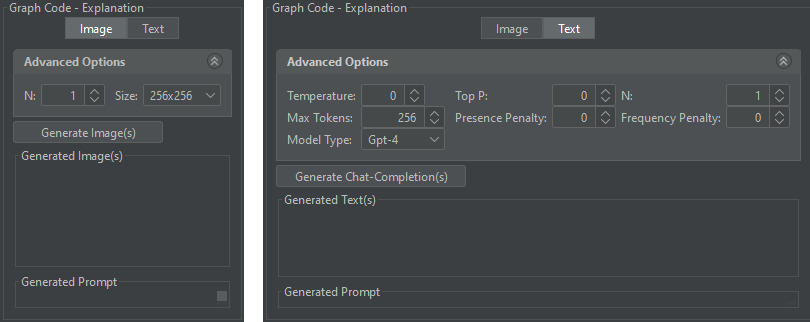
\includegraphics[width=\textwidth]{chapter/chapter_5/new-layouts-img-txt}
  \caption[Umordnung der Layouts von \textit{ImagePanel} und \textit{TextPanel}]{Umordnung der Layouts von \textit{ImagePanel} (links) und \textit{TextPanel} (rechts).}
  \label{sec5:eval:subsec:adaptation:fig:new-layouts}
\end{figure}

Das Beheben des dritten Mangels erfordert eine umfassendere Anpassung der Benutzeroberfläche, sowie eine Anpassung der Verarbeitung der generierten Ergebnisse.
Anstatt eines Labels zur Darstellung des generierten Bildes, bzw. eines Textfeldes zur Darstellung des generierten Textes, müssen nun mehrere Darstellungen in einer Benutzungsschnittstelle eingebunden werden.
Hierfür wird auf ein Registerkartenpanel \textit{JTabbedPane} anstelle des Labels \textit{JLabel} bzw. des Textfeldes \textit{JTextArea} zurückgegriffen.
Dieses Registerkartenpanel bietet das Darstellen mehrere Registerkarten mit eigenständigem Inhalt, sowie dem Hin- und Herschalten zwischen diesen Registerkarten.
Die Komponenten zur Darstellung der Inhalte bleiben unverändert ein \textit{JLabel} bzw. eine \textit{JTextArea}, die nun allerdings als Registerkarten dem Registerkartenpanel dynamisch hinzugefügt werden.
Das dynamische Hinzufügen erfolgt durch eine Anpassung der Verarbeitung, die in Bezug auf die Ergebnisse vorsieht, dass alle Datenelemente bzw. Inhalte einer Antwort durchlaufen werden.
\cref{sec5:eval:subsec:adaptation:fig:tabbedpane-image} zeigt die Darstellung mehrerer Registerkarten mit generierten Bildern in einem Registerkartenpanel in der Benutzungsschnittstelle \textit{ImagePanel}.

\begin{figure}[!ht]
  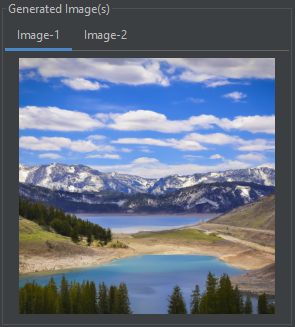
\includegraphics{chapter/chapter_5/tabbedpane-image}
  \caption{Registerkartenpanel in der Benutzungsschnittstelle \textit{ImagePanel} mit zwei Registerkarten.}
  \label{sec5:eval:subsec:adaptation:fig:tabbedpane-image}
\end{figure}

Das Beheben des letzten Mangels erfolgt durch das Modifizieren der Darstellung des Mauszeigers.
Eine geeignete Darstellung für einen Mauszeiger, der einen laufenden Hintergrundprozess darstellen soll, ist eine Sanduhr.
Die Modifikation dieser Darstellung kann in den entsprechenden Benutzungsschnittstellen \textit{ImagePanel} oder \textit{TextPanel} durch die Methode \textit{setCursor(...)} erfolgen.
In dem Moment, in dem ein Benutzer den Knopf \enquote{Generate ...} betätigt, wird im Hintergrund ein entsprechender Arbeitsprozess zum Generieren einer Erklärung begonnen und der Mauszeiger wird zu einer Sanduhr angepasst.
Sobald der Arbeitsprozess abgeschlossen wurde, erfolgreich oder nicht, wird der Mauszeiger auf den Standardwert zurückgesetzt.

Unabhängig von diesen Mängeln schlägt der Experte eine optionale Erweiterung der Benutzungsschnittstelle vor.
Um den Benutzern der Anwendung eine besseres Einordnen bzw. ein besseres in Bezug setzen der generierten Erklärungen zu den ursprünglichen Dateien zu ermöglichen, schlägt der Experte das Umsetzen einer Gegenüberstellung des entsprechenden Graph Codes, der Original-Datei und der generierten Erklärung vor.
Diese Gegenüberstellung wird erreicht durch das Hinzufügen einer Registerkartenpanels im rechten Teil des Grundbereichs \textit{EditorGraphCode} mit entsprechenden Registerkarten.
Diese Registerkarten sind zum einen die tabellarische Darstellung des Graph Codes, \textit{GraphCodeTable} und zum anderen eine neue Benutzungsschnittstelle \textit{OriginalAssetPanel}, die anhand des Dateinamens einer Graph Code Datei in der Kollektion nach einer entsprechenden Datei sucht und diese geeignet darstellt.
Hierfür kann zum Großteil auf bereits bestehenden Quellcode der Komponente \textit{AssetDetailPanel} zurückgegriffen werden.
\cref{sec5:eval:subsec:adaptation:fig:original-asset} zeigt die neue Benutzungsschnittstelle \textit{OriginalAssetPanel} zum Darstellen der originalen Datei.
Eine komplette Gegenüberstellung einer generierten visuellen Erklärung zu ihrer entsprechenden originalen Datei kann in \cref{sec5:eval:subsec:adaptation:fig:gc-orig-exp} eingesehen werden.

\begin{figure}[!ht]
  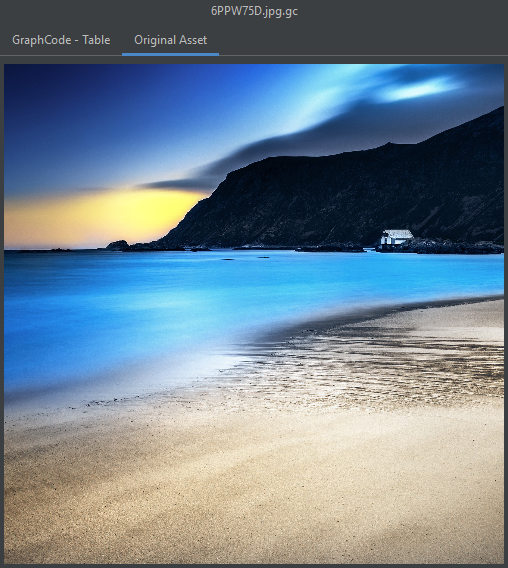
\includegraphics{chapter/chapter_5/original-asset}
  \caption{Ausgewählte Registerkarte mit der Darstellung der mit einem Graph Code ursprünglich assoziierten Datei.}
  \label{sec5:eval:subsec:adaptation:fig:original-asset}
\end{figure}

\begin{figure}[!ht]
  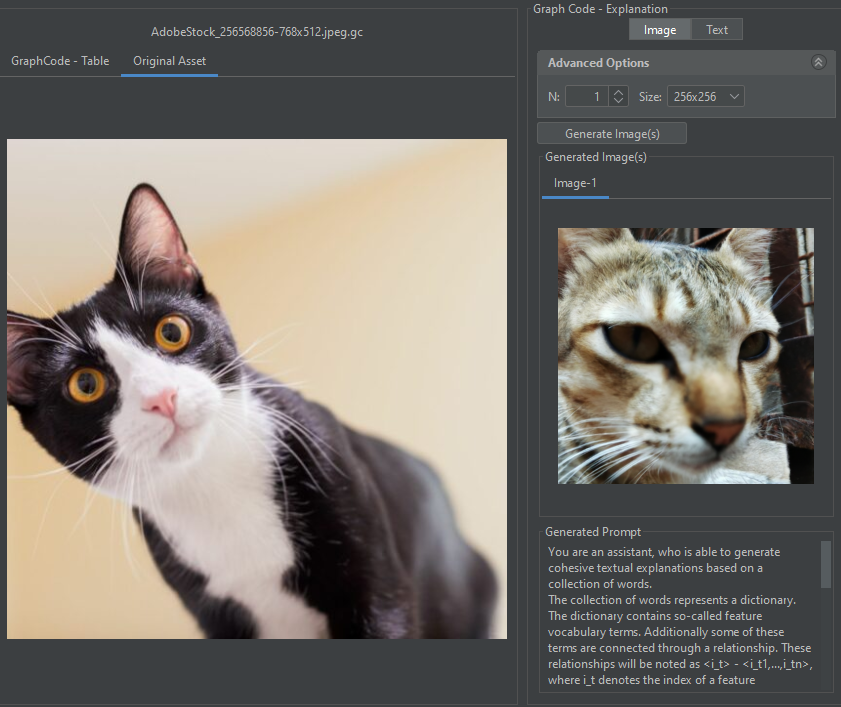
\includegraphics[width=\textwidth]{chapter/chapter_5/gc-orig-exp}
  \caption{Gegenüberstellung eines Graph Codes, der originalen Datei und der erzeugten visuellen Erklärung.}
  \label{sec5:eval:subsec:adaptation:fig:gc-orig-exp}
\end{figure}

Im Folgenden werden noch weitere Anpassungen an der prototypischen Proof-of-Concept Implementierung beschrieben, die unabhängig von den in der Evaluierung durchgeführten Experimenten erfolgten.

Im Umgang mit generativer KI sind Tokens von großer Bedeutung.
Es wurde daher in der Benutzungsschnittstelle \textit{TextPanel} eine Informationsoberfläche hinzugefügt, die es einem Benutzer ermöglicht, die Tokenanzahl eines generierten Textes einzusehen.
Darüber hinaus können durch diese Informationsoberfläche die Tokens in jenem Text farbig hervorgehoben werden.
Diese Anpassung kann \cref{sec5:eval:subsec:adaptation:fig:custom-token-info} eingesehen werden.

\begin{figure}[!ht]
  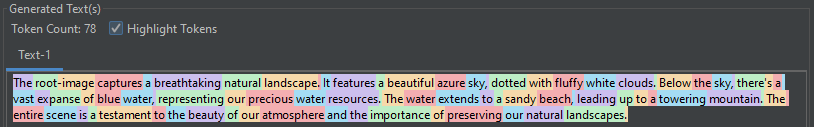
\includegraphics[width=\textwidth]{chapter/chapter_5/custom-token-info}
  \caption{Informationsoberfläche für Tokens in einem generierten Text.}
  \label{sec5:eval:subsec:adaptation:fig:custom-token-info}
\end{figure}

Eine weitere Anpassung, die eine sinnvolle Erweiterung der Funktionen der Anwendung darstellt, ist das automatische Sichern der in der Benutzungsschnittstelle \textit{ImagePanel} generierten Bilder in einem dafür vorgesehenen Ordner \enquote{explanations}.

% So wurde von OpenAI zum Zeitpunkt des Verfassens dieser Arbeit eine neue Version von Dall-E, Dall-E 3 \cite{dall-e-3}, vorgestellt, welches eine erhebliche Verbesserung zu vorherigen Systemen darstellen soll \cite{dall-e-3-paper}.

Infolge des angekündigten Updates \cite{openai-new-update-6_11_23} von OpenAI am 6. November 2023 (OpenAI DevDay \cite{openai-dev-day}) konnten weitere Anpassungen und Erweiterungen an der entwickelten Anwendung vorgenommen werden.
Dieses Update umfasst eine Reihe an Verbesserungen, Anpassungen und Erweiterungen.
Zu den Erweiterungen gehören die neue Dall-E 3 Schnittstelle, sowie eine Text-To-Speech (TTS, z.Dt. Text zu Sprache) Schnittstelle, mit welcher eine Audiodatei bzw. ein clip für einen beliebigen Text generiert werden kann.
Diese Neuerungen wurden ausgewählt und in die Anwendung integriert.
Die Integration dieser Erweiterungen äußert sich in einer Anpassung der Benutzungsschnittstelle \textit{ImagePanel} des Erklärungstyps Bild, welches hauptsächlich neue Auswahlmöglichkeiten in den erweiterten Optionen umfasst, sowie durch eine neue Benutzungsschnittstelle \textit{AudioPanel}, einsehbar in \cref{sec5:eval:subsubsec:adaptation:fig:audio-ui}, für einen neuen Erklärungstyp Audio, mit welchem auditive Erklärungen in Form von (kurzen) Audiodateien bzw. clips zu Graph Codes generiert werden können.
Aufgrund der Größe der durch Dall-E 3 generierten Bilder (1024x1024, 1792x1024, 1024x1792) können diese nicht mehr in der Benutzungsschnittstelle angezeigt werden und es wird stattdessen ein Knopf zum Öffnen des Bildes in einem externen Fenster angeboten.

\begin{figure}[!ht]
  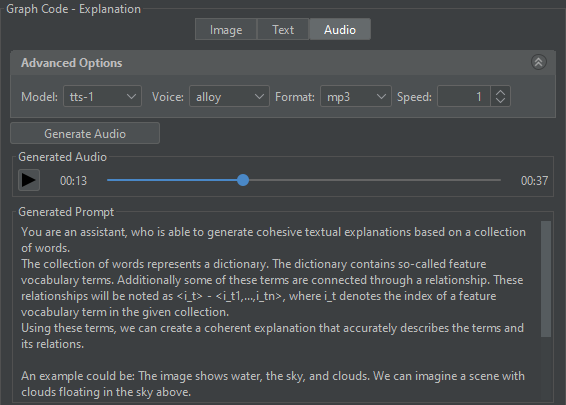
\includegraphics{chapter/chapter_5/right_audio_exp}
  \caption{Benutzungsschnittstelle für den Erklärungstyp Audio.}
  \label{sec5:eval:subsubsec:adaptation:fig:audio-ui}
\end{figure}

\clearpage

\subsection{Zusammenfassung}
\label{sec5:eval:subsec:summary}
Inhalt dieses Kapitels war die Evaluierung der im Rahmen der Implementierung entwickelten prototypischen Proof-of-Concept Implementierung.
In \cref{sec5:eval:subsec:eval-goals-methodology} wurden zuerst die Ziele der Evaluierung formuliert.
In Vorbereitung der Evaluierung wurden dann in \cref{sec5:eval:subsec:assign-exper} Aufgaben bzw. Experimente formuliert, die aus den Anwendungsfällen in \cref{sec3:model} abgeleitet wurden.
Diese Experimente wurden dann, der Methodik nach Nunamaker entsprechend, den Forschungszielen zugewiesen.
In den Forschungszielen FZ 1.4/E und FZ 2.4/E wurde dann jeweils die Vorbereitung, die Durchführung und die Einordnung der Ergebnisse des jeweiligen Experiments behandelt.
Die in diesen Forschungszielen gesammelten Erkenntnisse umfassen in erster Linie eine Reihe an Mängeln, die in der Durchführung der jeweiligen Experimente identifiziert werden konnten.
Als Reaktion auf diese Mängel wurden dann in \cref{sec5:eval:subsec:adaptation} Anpassungen an der Benutzungsschnittstelle und Funktionen der Anwendung beschrieben.

\subsubsection{Gewonnene Erkenntnisse}
In diesem Abschnitt werden die Erkenntnisse aus den Forschungszielen \enquote{FZ 1.4/E Erklärbarkeit von MMIR mittels generativer KI} und \enquote{FZ 2.4/E Integration generativer KI in das GMAF} zusammengefasst.

% Erkenntnisse aus FZ 1.4/E sammeln bzw. noch einmal kurz darstellen... (Hier auch die definierten Ziele der Evaluierung aufgreifen)
% Wurden Aspekte wie Vollständigkeit und Korrektheit durch die Evaluierungsmethodik abgedeckt und zu welchem Schluss kommt man nach der Durchführung des jeweiligen Experiments...?

In \cref{sec5:eval:subsec:fz-explainability} \enquote{FZ 1.4/E Erklärbarkeit von MMIR mittels generativer KI} konnte durch die Durchführung des Experiments \textbf{Exp. 1} festgestellt werden, dass die Anwendung eine Reihe an nicht fatalen Mängeln aufweist.
Nicht fatal soll ausdrücken, dass diese Mängel die Funktionen und Abläufe in dem Programm nicht negativ beeinträchtigen, sodass Benutzer der Anwendung ihre formulierten Ziele erreichen können.
Allerdings beeinträchtigen diese Mängel durchaus die Intuivität bzw. den Umgang mit dem Programm.
Zum Abschluss des Experiments wurden diese Mängel gesammelt, beschrieben und jeweils potentielle Lösungsvorschläge formuliert.
Auf die Ziele der Evaluierung rückblickend konnte festgehalten werden, dass beide Ziele, Vollständigkeit und Korrektheit der Implementierung, zufriedenstellend erfüllt wurden.

% Erkenntnisse aus FZ 2.4/E sammeln bzw. noch einmal kurz darstellen... (Hier auch die definierten Ziele der Evaluierung aufgreifen)
% Wurden Aspekte wie Vollständigkeit und Korrektheit durch die Evaluierungsmethodik abgedeckt und zu welchem Schluss kommt man nach der Durchführung des jeweiligen Experiments...?

In \cref{sec5:eval:subsec:fz-integration} \enquote{FZ 2.4/E Integration generativer KI in das GMAF} konnte durch die Durchführung des Experiments \textbf{Exp. 2} festgestellt werden, dass die Anwendung eine Reihe an nicht fatalen Mängeln aufweist.
Auch diese Mängel betreffen nicht die Funktionen und Abläufe des Programms, sondern beeinträchtigen nur die Intuivität bzw. den Umgang mit dem Programm.
Zum Abschluss des Experiments wurden diese Mängel gesammelt, beschrieben und jeweils potentielle Lösungsvorschläge formuliert.
Auf die Ziele der Evaluierung rückblickend konnte festgehalten werden, dass beide Ziele, Vollständigkeit und Korrektheit der Implementierung, zufriedenstellend erfüllt wurden.

Infolge der in den Experimenten identifizierten Mängel und den darauffolgend beschriebenen Lösungsvorschlägen wurden in \cref{sec5:eval:subsec:adaptation} Anpassungen an der prototypischen Proof-of-Concept Implementierung beschrieben, um diese Mängel zu beseitigen.
Diese Anpassungen variieren stark in ihrem Umfang, betreffen aber in erster Linie nur den Aufbau oder die Interaktion mit der Benutzungsschnittstelle.
Da keine fatalen Mängel festgestellt werden konnten, mussten keine Anpassungen an Datenmodell bezogene Algorithmen vorgenommen werden.

Darüber hinaus wurden, unabhängig von den in den Experimenten identifizierten Mängeln, in \cref{sec5:eval:subsec:adaptation} weitere Anpassungen und Erweiterungen von Funktionen der Anwendung beschrieben, die vom Experten vorgeschlagen oder vom Autor als sinnvoll erachtet wurden.

Aufgrund mangelnder Ressourcen konnte im Rahmen der Evaluierung keine umfassendere Prüfung der prototypischen Anwendung auf Fehler und Defekte durchgeführt werden.
Daher wurde mit den verfügbaren Ressourcen eine andere Evaluierungsmethodik durchgeführt, nach welchem für die Evaluierung festgehalten werden kann, dass die in dieser Arbeit entwickelte prototypische Proof-of-Concept Implementierung eine funktionierende Anwendung darstellt und welche das übergeordnete Ziel, Erklärungen von Graph Codes mittels generativer KI zu erzeugen, zufriedenstellend erfüllt.

Die nachfolgende Tabelle stellt eine Erweiterung der \cref{sec4:impl:subsec:summary:table:summary} dar und gibt eine Übersicht über den aktuellen Arbeitsstand nach Abschluss dieses Kapitels.

\begingroup
\def\arraystretch{1.1}%
\begin{xltabular}{\linewidth}{
            @{}
            >{
                \hsize=0.2\linewidth
                \raggedright\arraybackslash
            }X
            >{
                \hsize=0.6\linewidth
                \raggedright\arraybackslash
            }X
            >{
                \hsize=0.2\linewidth
            }X
            @{}
        }

        % First Header

        \caption{Tabelle zur Übersicht des aktuellen Arbeitsstands.}
        \label{sec5:eval:subsec:summary:table:summary}
        \\

        \toprule
        \multicolumn{3}{
            >{
                    \hsize=\linewidth\centering\arraybackslash
            }X
        }
        {
            \textbf{Forschungsziele}
        } \\ \midrule
        \textbf{FZ / OH} &  \textbf{Beschreibung} & \textbf{Referenz} \\ \midrule

        \endfirsthead

        \toprule
        \multicolumn{3}{
            >{
                    \hsize=\linewidth\centering\arraybackslash
            }X
        }
        {
            \textbf{Forschungsziele}
        } \\ \midrule
        \textbf{FZ / OH} & \textbf{Beschreibung} & \textbf{Referenz} \\ \midrule

        \endhead

        % Lower Rows

        \multicolumn{3}{
            >{
                    \hsize=\linewidth\centering\arraybackslash
            }X
        }
        {
            \textbf{Erklärbarkeit von MMIR mittels generativer KI}
        }
        \\
        \midrule

        FZ 1.1/O
        &
        Recherche zur Erklärbarkeit von MMIR mittels generativer KI
        \\

        &
        Grundlegende Technologien:
        &

        \\

        &
        \tabitem GMAF
        &
        \cref{sec2:sota:subsubsec:gmaf}
        \\

        &
        \tabitem MMFG
        &
        \cref{sec2:sota:subsubsec:mmfg}
        \\

        &
        \tabitem Graph Code
        &
        \cref{sec2:sota:subsubsec:graph-codes}
        \\

        % Offene Herausforderungen aus FZ1/O

        OH 1.1
        &
        Erste offene Herausforderung
        &
        \hyperref[sec2:sota:oi:1.1]{\textbf{OH 1.1}}
        \\


        &
        Systeme generativer KI und ein Überlick über aktuelle Systeme
        &
        \cref{sec2:sota:subsubsec:genai}
        \\

        &
        Diskussion und Auswahl von Systemen
        &
        \cref{sec2:sota:subsubsec:fz1:discussion}
        \\

        OH 1.2
        &
        Zweite offene Herausforderung
        &
        \hyperref[sec2:sota:oi:2.1]{\textbf{OH 2.1}}
        \\

        \midrule

        FZ 1.2/TB
        &
        Modellierung der Erklärbarkeit von MMIR mittels generativer KI
        &

        \\

        &
        Erklärbarkeit durch generative KI
        &
        \cref{sec3:model:subsubsec:explainability-through-genai}
        \\

        &
        $\rightarrow$ Behandlung der ersten offenen Herausforderung \hyperref[sec2:sota:oi:1.1]{\textbf{OH 1.1}}
        &
        \\

        &
        Anwendungsfälle:
        &
        \cref{sec3:model:subsubsec:use-cases}
        \\

        &
        \tabitem Textuelle Beschreibungen
        &
        %\cref{sec3:model:par:textual-desc-use-cases}
        \\

        &
        Wireframes
        &
        \cref{sec3:model:par:wireframe}
        \\

        &
        Mechanismen
        &
        \cref{sec3:model:par:mechanism-use-cases}
        \\

        &
        Sequenzdiagramme
        &
        \cref{sec3:model:par:seq-use-cases}
        \\

        &
        $\rightarrow$ Behandlung der zweiten offenen Herausforderung \hyperref[sec2:sota:oi:1.2]{\textbf{OH 1.2}}
        &
        \\

        \midrule

        FZ 1.3/I
        &
        Implementierung der Erklärbarkeit von MMIR mittels generativer KI
        &

        \\

        &
        Benutzungsschnittstelle:
        &
        \cref{sec4:impl:subsubsec:ui}
        \\

        &
        \tabitem Elemente der Benutzeroberfläche
        &
        \\

        &
        \tabitem Interaktion mit der Benutzeroberfläche
        &
        \\

        \midrule

        FZ 1.4/E
        &
        Evaluierung der Erklärbarkeit von MMIR mittels generativer KI
        &

        \\

        &
        Experiment \textbf{Exp. 1}:
        &
        \\

        &
        \tabitem Vorbereitung des Experiments
        &
        \cref{sec5:eval:subsubsec:exp-1:preparation}
        \\

        &
        \tabitem Durchführung des Experiments
        &
        \cref{sec5:eval:subsubsec:exp-1:execution}
        \\

        &
        \tabitem Erkenntnisse des Experiments
        &
        \cref{sec5:eval:subsubsec:exp-1:results-discussion}
        \\

        \midrule

        \multicolumn{3}{
            >{
                    \hsize=\linewidth\centering\arraybackslash
            }X
        }
        {
            \textbf{Integration generativer KI in das GMAF}
        }
        \\
        \midrule

        FZ 2.1/O
        &
        Recherche zur Integration generativer KI in das GMAF
        &

        \\


        &
        Aufzeigen der Integrationsmöglichkeiten von:
        &

        \\

        &
        \tabitem Graph Codes
        &
        \cref{sec2:sota:subsubsec:gc-capabilities-integration}
        \\

        &
        Erste offene Herausforderung
        &
        \hyperref[sec2:sota:oi:2.1]{\textbf{OH 2.1}}
        \\

        &
        \tabitem Systemen generativer KI
        &
        \cref{sec2:sota:subsubsec:genai-capabilities-integration}
        \\

        &
        Zweite offene Herausforderung
        &
        \hyperref[sec2:sota:oi:2.2]{\textbf{OH 2.2}}
        \\

        \midrule

        FZ 2.2/TB
        &
        Modellierung der Integration generativer KI in das GMAF
        &

        \\

        &
        Transformation von Graph Codes
        &
        \cref{sec3:model:subsubsec:gc-transformation}
        \\

        &
        \tabitem Transformation des Vokabulars
        &
        \\

        &
        \tabitem Transformation der Matrix
        &
        \\

        &
        \tabitem Anwendung von Graph Code Metriken
        &
        \\

        &
        $\rightarrow$ Behandlung der ersten offenen Herausforderung \hyperref[sec2:sota:oi:2.1]{\textbf{OH 2.1}}
        &
        \\

        &
        Einbindung generativer KI in das GMAF
        &
        \cref{sec3:model:subsubsec:genai-integration}
        \\

        &
        $\rightarrow$ Behandlung der zweiten offenen Herausforderung \hyperref[sec2:sota:oi:2.2]{\textbf{OH 2.2}}
        &
        \\

        \midrule

        FZ 2.3/I
        &
        Implementierung der Integration generativer KI in das GMAF
        &

        \\

        &
        Transformation von Graph Codes
        &
        \cref{sec4:impl:subsubsec:gc-transformation}
        \\

        &
        Integration der Endpunkte
        &
        \cref{sec4:impl:subsubsec:endpoint-integration}
        \\

        \midrule

        FZ 2.4/E
        &
        Evaluierung der Integration generativer KI in das GMAF
        &

        \\

        &
        Experiment \textbf{Exp. 2}:
        &
        \\

        &
        \tabitem Vorbereitung des Experiments
        &
        \cref{sec5:eval:subsubsec:exp-2:preparation}
        \\

        &
        \tabitem Durchführung des Experiments
        &
        \cref{sec5:eval:subsubsec:exp-2:execution}
        \\

        &
        \tabitem Erkenntnisse des Experiments
        &
        \cref{sec5:eval:subsubsec:exp-2:results-discussion}
        \\

        \bottomrule
\end{xltabular}
\endgroup


Im nächsten \cref{sec6:disc} \enquote{Zusammenfassung} wird die gesamte Arbeit zusammengefasst, auf die Forschungsfragen aus dem ersten Kapitel zurückgesprungen und weitere Informationen in Bezug auf diese Arbeit beschrieben.


%\section{Diskussion}
\label{sec6:disc}

\appendix

\section{Anhang}

%%\vspace*{\fill}
\begin{center}
\begin{turn}{-90}
\begin{sideways}
    \centering
    \begin{minipage}{\linewidth}
    \captionsetup{type=figure}
    \resizebox{0.75\linewidth}{!}{
    \begin{ganttchart}[y unit title=0.6cm,
            y unit chart=0.8cm,
            x unit=0.4cm,
            vgrid,hgrid, 
            title label anchor/.style={below=-1.6ex},
            title left shift=.05,
            title right shift=-.06,
            title height=1,
            progress label text={},
            bar height=0.4,
            bar top shift=0.3,
            %bar node/.append style={anchor=north},
            bar label node/.append style={align=left, text width=7em, left=3pt},
            milestone label node/.append style={align=left, text width=9em},
            milestone inline label node/.append style={right=2ex,fill=white,fill opacity=.75,text opacity=1},
            flip/.style={milestone inline label node/.append style={left=2ex}},
            group right shift=0,
            group top shift=.6,
            group height=0.3]{1}{21}
    %labels
    \gantttitle{Arbeits- und Zeitplan}{21} \\
    %\gantttitle{April}{8}
    %\gantttitle{Mai}{8}
    %\gantttitle{Juni}{8}
    %\gantttitle{Juli}{8} \\
    \gantttitle[title label node/.append style={xshift=-18.8mm}]{Kalenderwoche}{0}
    %\foreach \x in {14,...,29} {
    %    \gantttitle{\x}{2}
    %}
    \gantttitle{14-17}{4}
    \gantttitle{18-30}{5}
    \gantttitle{31-34}{4}
    \gantttitle{35-38}{4}
    \gantttitle{39-42}{4}
    
    \\
        
    %tasks
    
    \ganttbar{Einleitung}{1}{3} \\
    \ganttbar{FZ 1.1/0}{4}{6} \\
    \ganttbar{FZ 2.1/0}{7}{9}
    \ganttmilestone[inline]{\textbf{Beobachtung}}{9} \\
    \ganttbar{FZ 1.2/TB}{10}{11} \\
    \ganttbar{FZ 2.2/TB}{12}{13}
    \ganttmilestone[inline]{\textbf{Modellierung}}{13} \\
    \ganttbar{FZ 1.3/I}{14}{15} \\
    \ganttbar{FZ 2.3/I}{16}{17} \\
    \ganttmilestone[inline,flip]{\textbf{Implememtierung}}{17} \\
    \ganttbar{FZ 1.4/E}{18}{19} \\
    \ganttbar{FZ 2.4/E}{20}{21} \\
    \ganttmilestone[inline,flip]{\textbf{Experiment}}{21} 
        
    %relations 
    \ganttlink{elem0}{elem1}
    \ganttlink{elem1}{elem2}
    %\ganttlink{elem1}{elem3}
    \ganttlink{elem3}{elem4}
    \ganttlink{elem4}{elem5}
    \ganttlink{elem6}{elem7}
    \ganttlink{elem7}{elem8}
    \ganttlink{elem8}{elem10}
    %\ganttlink{elem9}{elem10}
    \ganttlink{elem10}{elem11}
        
    \end{ganttchart}
    }
    \captionof{figure}{Arbeits- und Zeitplan.} \label{sec1:intro:fig:gantt-chart-timeline}
    \end{minipage}
\end{sideways}
\end{turn}
\end{center}
\vspace*{\fill}


%\begin{figure}[!htb]
    \centering
    \copyrightbox[b]{
            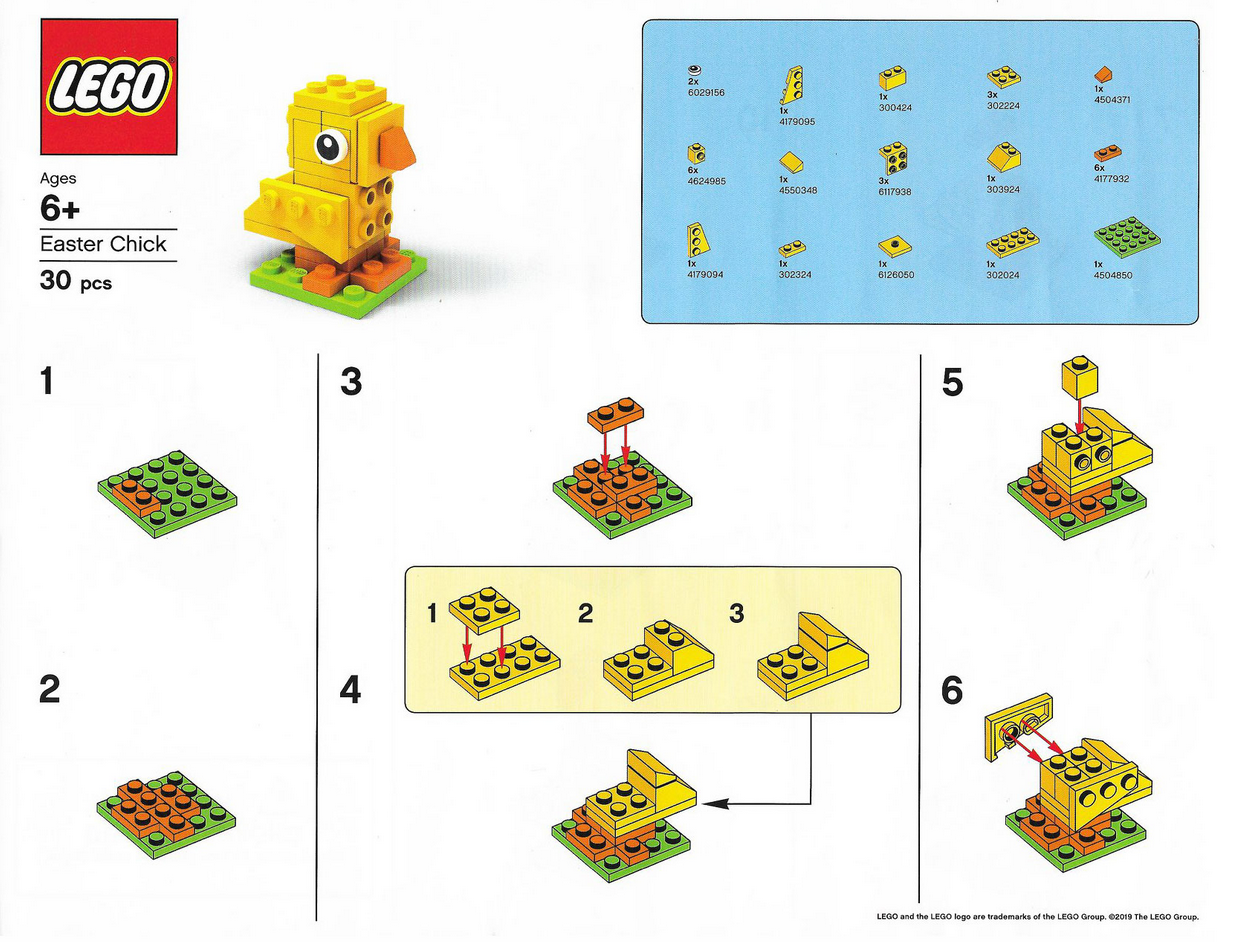
\includegraphics[width=0.8\linewidth]{resources/images/lego-instructions.png}
        }
        {%
        \textcolor{black}{%
            %Haftungsausschluss: \copyright{} 2023 Lego Gruppe - Diese Arbeit ist unabhängig und wurde von der LEGO Gruppe weder genehmigt noch gesponsert.
            Haftungsausschluss: LEGO \textsuperscript{\textregistered{}} und das LEGO Logo sind Marken der LEGO Unternehmensgruppe. 
            \newline
            \copyright{} 2023 Lego Gruppe. Diese Arbeit ist unabhängig und wurde von der LEGO Gruppe weder genehmigt, noch gesponsort.
        }
    }
    \caption{Bauanleitung für ein Lego-Set \cite{lego-easter-chick}.}
    \label{sec1:intro:subsec:problems:fig:lego-instructions}
\end{figure}

\setcounter{biburllcpenalty}{7000}
\setcounter{biburlucpenalty}{8000}
\emergencystretch=3em
{
    \RaggedRight
    \printbibliography
}

\end{document}
